% Options for packages loaded elsewhere
\PassOptionsToPackage{unicode}{hyperref}
\PassOptionsToPackage{hyphens}{url}
\PassOptionsToPackage{dvipsnames,svgnames,x11names}{xcolor}
%
\documentclass[
  letterpaper,
  DIV=11,
  numbers=noendperiod]{scrreprt}

\usepackage{amsmath,amssymb}
\usepackage{iftex}
\ifPDFTeX
  \usepackage[T1]{fontenc}
  \usepackage[utf8]{inputenc}
  \usepackage{textcomp} % provide euro and other symbols
\else % if luatex or xetex
  \usepackage{unicode-math}
  \defaultfontfeatures{Scale=MatchLowercase}
  \defaultfontfeatures[\rmfamily]{Ligatures=TeX,Scale=1}
\fi
\usepackage{lmodern}
\ifPDFTeX\else  
    % xetex/luatex font selection
\fi
% Use upquote if available, for straight quotes in verbatim environments
\IfFileExists{upquote.sty}{\usepackage{upquote}}{}
\IfFileExists{microtype.sty}{% use microtype if available
  \usepackage[]{microtype}
  \UseMicrotypeSet[protrusion]{basicmath} % disable protrusion for tt fonts
}{}
\makeatletter
\@ifundefined{KOMAClassName}{% if non-KOMA class
  \IfFileExists{parskip.sty}{%
    \usepackage{parskip}
  }{% else
    \setlength{\parindent}{0pt}
    \setlength{\parskip}{6pt plus 2pt minus 1pt}}
}{% if KOMA class
  \KOMAoptions{parskip=half}}
\makeatother
\usepackage{xcolor}
\ifLuaTeX
  \usepackage{luacolor}
  \usepackage[soul]{lua-ul}
\else
  \usepackage{soul}
  
\fi
\setlength{\emergencystretch}{3em} % prevent overfull lines
\setcounter{secnumdepth}{5}
% Make \paragraph and \subparagraph free-standing
\ifx\paragraph\undefined\else
  \let\oldparagraph\paragraph
  \renewcommand{\paragraph}[1]{\oldparagraph{#1}\mbox{}}
\fi
\ifx\subparagraph\undefined\else
  \let\oldsubparagraph\subparagraph
  \renewcommand{\subparagraph}[1]{\oldsubparagraph{#1}\mbox{}}
\fi

\usepackage{color}
\usepackage{fancyvrb}
\newcommand{\VerbBar}{|}
\newcommand{\VERB}{\Verb[commandchars=\\\{\}]}
\DefineVerbatimEnvironment{Highlighting}{Verbatim}{commandchars=\\\{\}}
% Add ',fontsize=\small' for more characters per line
\usepackage{framed}
\definecolor{shadecolor}{RGB}{241,243,245}
\newenvironment{Shaded}{\begin{snugshade}}{\end{snugshade}}
\newcommand{\AlertTok}[1]{\textcolor[rgb]{0.68,0.00,0.00}{#1}}
\newcommand{\AnnotationTok}[1]{\textcolor[rgb]{0.37,0.37,0.37}{#1}}
\newcommand{\AttributeTok}[1]{\textcolor[rgb]{0.40,0.45,0.13}{#1}}
\newcommand{\BaseNTok}[1]{\textcolor[rgb]{0.68,0.00,0.00}{#1}}
\newcommand{\BuiltInTok}[1]{\textcolor[rgb]{0.00,0.23,0.31}{#1}}
\newcommand{\CharTok}[1]{\textcolor[rgb]{0.13,0.47,0.30}{#1}}
\newcommand{\CommentTok}[1]{\textcolor[rgb]{0.37,0.37,0.37}{#1}}
\newcommand{\CommentVarTok}[1]{\textcolor[rgb]{0.37,0.37,0.37}{\textit{#1}}}
\newcommand{\ConstantTok}[1]{\textcolor[rgb]{0.56,0.35,0.01}{#1}}
\newcommand{\ControlFlowTok}[1]{\textcolor[rgb]{0.00,0.23,0.31}{#1}}
\newcommand{\DataTypeTok}[1]{\textcolor[rgb]{0.68,0.00,0.00}{#1}}
\newcommand{\DecValTok}[1]{\textcolor[rgb]{0.68,0.00,0.00}{#1}}
\newcommand{\DocumentationTok}[1]{\textcolor[rgb]{0.37,0.37,0.37}{\textit{#1}}}
\newcommand{\ErrorTok}[1]{\textcolor[rgb]{0.68,0.00,0.00}{#1}}
\newcommand{\ExtensionTok}[1]{\textcolor[rgb]{0.00,0.23,0.31}{#1}}
\newcommand{\FloatTok}[1]{\textcolor[rgb]{0.68,0.00,0.00}{#1}}
\newcommand{\FunctionTok}[1]{\textcolor[rgb]{0.28,0.35,0.67}{#1}}
\newcommand{\ImportTok}[1]{\textcolor[rgb]{0.00,0.46,0.62}{#1}}
\newcommand{\InformationTok}[1]{\textcolor[rgb]{0.37,0.37,0.37}{#1}}
\newcommand{\KeywordTok}[1]{\textcolor[rgb]{0.00,0.23,0.31}{#1}}
\newcommand{\NormalTok}[1]{\textcolor[rgb]{0.00,0.23,0.31}{#1}}
\newcommand{\OperatorTok}[1]{\textcolor[rgb]{0.37,0.37,0.37}{#1}}
\newcommand{\OtherTok}[1]{\textcolor[rgb]{0.00,0.23,0.31}{#1}}
\newcommand{\PreprocessorTok}[1]{\textcolor[rgb]{0.68,0.00,0.00}{#1}}
\newcommand{\RegionMarkerTok}[1]{\textcolor[rgb]{0.00,0.23,0.31}{#1}}
\newcommand{\SpecialCharTok}[1]{\textcolor[rgb]{0.37,0.37,0.37}{#1}}
\newcommand{\SpecialStringTok}[1]{\textcolor[rgb]{0.13,0.47,0.30}{#1}}
\newcommand{\StringTok}[1]{\textcolor[rgb]{0.13,0.47,0.30}{#1}}
\newcommand{\VariableTok}[1]{\textcolor[rgb]{0.07,0.07,0.07}{#1}}
\newcommand{\VerbatimStringTok}[1]{\textcolor[rgb]{0.13,0.47,0.30}{#1}}
\newcommand{\WarningTok}[1]{\textcolor[rgb]{0.37,0.37,0.37}{\textit{#1}}}

\providecommand{\tightlist}{%
  \setlength{\itemsep}{0pt}\setlength{\parskip}{0pt}}\usepackage{longtable,booktabs,array}
\usepackage{calc} % for calculating minipage widths
% Correct order of tables after \paragraph or \subparagraph
\usepackage{etoolbox}
\makeatletter
\patchcmd\longtable{\par}{\if@noskipsec\mbox{}\fi\par}{}{}
\makeatother
% Allow footnotes in longtable head/foot
\IfFileExists{footnotehyper.sty}{\usepackage{footnotehyper}}{\usepackage{footnote}}
\makesavenoteenv{longtable}
\usepackage{graphicx}
\makeatletter
\def\maxwidth{\ifdim\Gin@nat@width>\linewidth\linewidth\else\Gin@nat@width\fi}
\def\maxheight{\ifdim\Gin@nat@height>\textheight\textheight\else\Gin@nat@height\fi}
\makeatother
% Scale images if necessary, so that they will not overflow the page
% margins by default, and it is still possible to overwrite the defaults
% using explicit options in \includegraphics[width, height, ...]{}
\setkeys{Gin}{width=\maxwidth,height=\maxheight,keepaspectratio}
% Set default figure placement to htbp
\makeatletter
\def\fps@figure{htbp}
\makeatother
% definitions for citeproc citations
\NewDocumentCommand\citeproctext{}{}
\NewDocumentCommand\citeproc{mm}{%
  \begingroup\def\citeproctext{#2}\cite{#1}\endgroup}
\makeatletter
 % allow citations to break across lines
 \let\@cite@ofmt\@firstofone
 % avoid brackets around text for \cite:
 \def\@biblabel#1{}
 \def\@cite#1#2{{#1\if@tempswa , #2\fi}}
\makeatother
\newlength{\cslhangindent}
\setlength{\cslhangindent}{1.5em}
\newlength{\csllabelwidth}
\setlength{\csllabelwidth}{3em}
\newenvironment{CSLReferences}[2] % #1 hanging-indent, #2 entry-spacing
 {\begin{list}{}{%
  \setlength{\itemindent}{0pt}
  \setlength{\leftmargin}{0pt}
  \setlength{\parsep}{0pt}
  % turn on hanging indent if param 1 is 1
  \ifodd #1
   \setlength{\leftmargin}{\cslhangindent}
   \setlength{\itemindent}{-1\cslhangindent}
  \fi
  % set entry spacing
  \setlength{\itemsep}{#2\baselineskip}}}
 {\end{list}}
\usepackage{calc}
\newcommand{\CSLBlock}[1]{\hfill\break\parbox[t]{\linewidth}{\strut\ignorespaces#1\strut}}
\newcommand{\CSLLeftMargin}[1]{\parbox[t]{\csllabelwidth}{\strut#1\strut}}
\newcommand{\CSLRightInline}[1]{\parbox[t]{\linewidth - \csllabelwidth}{\strut#1\strut}}
\newcommand{\CSLIndent}[1]{\hspace{\cslhangindent}#1}

\usepackage{booktabs}
\usepackage{longtable}
\usepackage{array}
\usepackage{multirow}
\usepackage{wrapfig}
\usepackage{float}
\usepackage{colortbl}
\usepackage{pdflscape}
\usepackage{tabu}
\usepackage{threeparttable}
\usepackage{threeparttablex}
\usepackage[normalem]{ulem}
\usepackage{makecell}
\usepackage{xcolor}
\KOMAoption{captions}{tableheading}
\makeatletter
\@ifpackageloaded{bookmark}{}{\usepackage{bookmark}}
\makeatother
\makeatletter
\@ifpackageloaded{caption}{}{\usepackage{caption}}
\AtBeginDocument{%
\ifdefined\contentsname
  \renewcommand*\contentsname{Table of contents}
\else
  \newcommand\contentsname{Table of contents}
\fi
\ifdefined\listfigurename
  \renewcommand*\listfigurename{List of Figures}
\else
  \newcommand\listfigurename{List of Figures}
\fi
\ifdefined\listtablename
  \renewcommand*\listtablename{List of Tables}
\else
  \newcommand\listtablename{List of Tables}
\fi
\ifdefined\figurename
  \renewcommand*\figurename{Figure}
\else
  \newcommand\figurename{Figure}
\fi
\ifdefined\tablename
  \renewcommand*\tablename{Table}
\else
  \newcommand\tablename{Table}
\fi
}
\@ifpackageloaded{float}{}{\usepackage{float}}
\floatstyle{ruled}
\@ifundefined{c@chapter}{\newfloat{codelisting}{h}{lop}}{\newfloat{codelisting}{h}{lop}[chapter]}
\floatname{codelisting}{Listing}
\newcommand*\listoflistings{\listof{codelisting}{List of Listings}}
\makeatother
\makeatletter
\makeatother
\makeatletter
\@ifpackageloaded{caption}{}{\usepackage{caption}}
\@ifpackageloaded{subcaption}{}{\usepackage{subcaption}}
\makeatother
\ifLuaTeX
  \usepackage{selnolig}  % disable illegal ligatures
\fi
\usepackage{bookmark}

\IfFileExists{xurl.sty}{\usepackage{xurl}}{} % add URL line breaks if available
\urlstyle{same} % disable monospaced font for URLs
\hypersetup{
  pdftitle={Assignment Statistics KVHEM CZU SS 2024},
  pdfauthor={MSc. Friederike Johanna Rosa Wölke},
  colorlinks=true,
  linkcolor={blue},
  filecolor={Maroon},
  citecolor={Blue},
  urlcolor={Blue},
  pdfcreator={LaTeX via pandoc}}

\title{Assignment Statistics KVHEM CZU SS 2024}
\author{MSc. Friederike Johanna Rosa Wölke}
\date{2024-07-04}

\begin{document}
\maketitle

\renewcommand*\contentsname{Table of contents}
{
\hypersetup{linkcolor=}
\setcounter{tocdepth}{2}
\tableofcontents
}
\bookmarksetup{startatroot}

\chapter*{Assignment for PhD Statistics class
2024}\label{assignment-for-phd-statistics-class-2024}
\addcontentsline{toc}{chapter}{Assignment for PhD Statistics class 2024}

\markboth{Assignment for PhD Statistics class 2024}{Assignment for PhD
Statistics class 2024}

\begin{center}\rule{0.5\linewidth}{0.5pt}\end{center}

\section*{\texorpdfstring{\textbf{Topic of Credit Report -- Statistical
Methods} - Prague,
07.05.2024}{Topic of Credit Report -- Statistical Methods - Prague, 07.05.2024}}\label{topic-of-credit-report-statistical-methods---prague-07.05.2024}
\addcontentsline{toc}{section}{\textbf{Topic of Credit Report --
Statistical Methods} - Prague, 07.05.2024}

\markright{\textbf{Topic of Credit Report -- Statistical Methods} -
Prague, 07.05.2024}

\ul{Title of report:} \emph{Towards predicting temporal biodiversity
change from static patterns}

\ul{Name:} MSc. Friederike Wölke

\ul{Supervisor:} Dr.~Petr Keil

\ul{Thesis title:} Universal imprints of temporal change in static
spatial patterns of biodiversity

\ul{Expected methods applied:}

\begin{itemize}
\tightlist
\item
  Machine learning {(random forest regression from ranger package; using
  the caret suite of tools for hyperparameter tuning)}
\item
  visualization of results (ggplot2, partial plots, BAM chart).
\end{itemize}

\ul{Abstract:}

The world is undergoing significant environmental transformations,
impacting biodiversity and ecosystem functions. Since obtaining temporal
replication of biodiversity data is challenging due to cost and
monitoring limitations, I aim at predicting temporal trends in species
occupancy without requiring temporally replicated data.

Biodiversity kinetics leave characteristics imprint in the spatial
patterns that we can see from geo-referenced presence/absence data
because the underlying processes such as extinction and colonization
happen across space.

I aim at predicting the log ratio of temporal change in occupancy (i.e.,
the sum of area occupied by a species) between two sampling periods from
a set of predictor variables that are either related to \textbf{H1)
species traits and ecology}, \textbf{H2)~ geometric features of the
species range from a single sampling period}, \textbf{H3) biodiversity
equilibrium dynamics via spatial diversity patterns},~ or \textbf{H4) to
the characteristics of the study region} -- all of which may equally
contribute and act in concert to explaining the temporal process that is
underlying the spatial pattern.

For this I use high-quality, spatially continuous atlas data from four
breeding bird atlases from temperate zones across the globe. Atlas data
comes with spatial grids that enable easy up- and down scaling of the
data.

Here, I assess universal imprints of temporal change in breeding birds
in Czech Republic, Japan, New York State and the whole of Europe across
two aggregated sampling periods that took place pre-2000 and post-2000.
Since data for two sampling periods are available, I will additionally
test whether imprints in the spatial aggregation of species can better
predict past or future biodiversity change.

For this, I collated 60 predictor variables that vary across sampling
periods - each belonging to one of the hypotheses mentioned above. I
will use random forest regression to determine the capability of static
patterns to predict temporal change, identify the most important
predictor variables and compare observed versus predicted results.

If my model can predict temporal change from static patterns, this
method will be a useful tool for estimating temporal change in areas and
for species where repeated monitoring might not be feasible. If the
models are only partially able to predict temporal trends, the important
predictors may still yield insights into how temporal processes are
acting across space. Additionally disentangling whether imprints of
biodiversity kinetics are better at explaining past versus future change
may help to understand the temporal dimensions of the imprints.

\includegraphics{_img/VisualAbstract1_good.png}

\section*{Adjustments to the topic}\label{adjustments-to-the-topic}
\addcontentsline{toc}{section}{Adjustments to the topic}

\markright{Adjustments to the topic}

Since handing in the topic of the report, I found that the response
variable that I chose did not capture much of a signal in the data which
led to very poor predictive power and model performances. The
distribution of this variable was predominantly centered around zero
with few extreme cases of extreme increase or decrease, while predictor
variables varied heavily. Ths suggested that there is just not enough
signal in the \emph{log ratio} for predictions. I investigated why this
was the case. Here follows the explanation:

Log ratio of the area of occupancy (\emph{log ratio AOO}) was calculated
as follows:\\
log times the product of the sum of all areas occupied in sampling
period 2 (AOO 2) divided by the sum of all areas occupied in sampling
period 1 (AOO1 ), i.e.,:\\
\[log Ratio_{1,2} = log(AOO_{tp2}/AOO_{tp1})\]

I found that most species did not experience much change in AOO between
both sampling periods, but a lot of site turnover happened. This means
that, although \emph{log ratio of AOO} is zero, species moved around a
lot. Some even switched from a north Europe-based distribution to a
south Europe-based distribution (e.g.~\emph{Vanellus vanellus}, the
Northern Lapwing).

\includegraphics{_img/ChangeMaps2.png}

These changes were not detected at all by the metric that I chose to
describe temporal change. Thus I decided to include another metric of
temporal change which better captures the spatial change that species
undergo. I calculated the \emph{Jaccard index of similarity} for each
species across their occupied sites between two sampling periods.
\emph{Jaccard} was calculated as follows:

\[
J(X,Y) = |X∩Y| / |X∪Y|
\]

where \(X\) are the names of the cells that are occupied in period 1 and
\(Y\) is the names of the cells that are occupied in period 2. This
results in a measure of similarity between sites that ranges from 1 (=
complete similarity in sites) to 0 (= no similar sites). This may give
an idea of how much spatial change happened for each species across
sampling periods.

In the following report I will still report the results for \emph{log
ratio AOO}, but these will have secondary importance and results for
different response variables will be printed in separate tabs for the
same analysis.

\bookmarksetup{startatroot}

\chapter{Script 1 - Data preparation}\label{script-1---data-preparation}

\bookmarksetup{startatroot}

\chapter{The Analysis}\label{the-analysis}

I will start by sourcing some functions that I have wrote to simplify my
code. The first is \texttt{load\_and\_install()} and it's supposed to
suppress the start messages from the packages while installing and
loading all packages that are not already installed and loaded.

\section{Source custom functions}

\begin{Shaded}
\begin{Highlighting}[]
\FunctionTok{rm}\NormalTok{(}\AttributeTok{list =} \FunctionTok{ls}\NormalTok{())}
\FunctionTok{source}\NormalTok{(}\StringTok{"../src/functions.R"}\NormalTok{)}
\end{Highlighting}
\end{Shaded}

\section{MachineLearning packages}

\begin{Shaded}
\begin{Highlighting}[]
\NormalTok{pckgs }\OtherTok{\textless{}{-}} \FunctionTok{c}\NormalTok{(}\StringTok{"dplyr"}\NormalTok{, }\StringTok{"ggplot2"}\NormalTok{, }\StringTok{"reshape2"}\NormalTok{, }
           \StringTok{"ggcorrplot"}\NormalTok{, }
           \StringTok{"caret"}\NormalTok{,  }\StringTok{"recipes"}\NormalTok{,   }\StringTok{"caretEnsemble"}\NormalTok{, }
           \StringTok{"randomForest"}\NormalTok{, }\StringTok{"ranger"}\NormalTok{, }\StringTok{"gbm"}\NormalTok{, }\StringTok{"xgboost"}\NormalTok{, }
           \StringTok{"vegan"}\NormalTok{, }\StringTok{"pdp"}\NormalTok{, }
           \StringTok{"gridExtra"}\NormalTok{, }\StringTok{"kableExtra"}\NormalTok{)}

\FunctionTok{install\_and\_load}\NormalTok{(pckgs)}
\end{Highlighting}
\end{Shaded}

\section{The data}\label{the-data}

Since the raw data is not open, I am providing the (reduced) predictor
table that I calculated from it and other external data. For additional
information on how the raw data was handled to produce this set of
predictors, please visit the corresponding github repository
(\url{https://github.com/FriedaRosa/BEAST_General_Procedures/tree/main/Project_Frieda/StaticPredictors}).

The data has bird species in rows (\texttt{verbatim\_name}) and their
predictor data across different datasets (\texttt{dataset}) in columns.

The column \texttt{log\_R2\_1} is the \emph{log ratio of AOO (area of
occupancy)} between two sampling periods (indicated with
\texttt{tp\ =\ 1} or \texttt{tp\ =\ 2}) and was the inital response for
my temporal change models.

\texttt{Telfer\_1\_2} is another measure of temporal change, though it
is relative for each species in a dataset in comparison to the average
other species. Telfer will not be further investigated in this
assignment. I have assessed its correlation with \emph{log ratio} before
and they correlate well.

\texttt{Jaccard} is the Jaccard index of similarity and indicates how
similar ( 0 - 1) two species ranges are across different sampling
periods.

\textbf{Raw data:}

\begin{itemize}
\item
  Bird Atlases:(Council 2022; Keller et al. 2020; Ministry of the
  Environment, Natural Environment Bureau, Biodiversity Center 2004; New
  York State Department of Environmental Conservation 1980-1985,
  2000-2005; Šťastný, Bejček, and Hudec 1997, 2006; Ueda and Uemura
  2021)
\item
  External Data:(Hagemeyer, Blair, and Loos 2016; Hagemeijer and Blair
  1997; Karger et al. 2017a, 2017b; BirdLife International 2020; Tobias
  et al. 2022)
\end{itemize}

\bookmarksetup{startatroot}

\chapter{Preparations}\label{preparations}

\section{Data handling}\label{data-handling}

Here I'm excluding some predictors which are overlapping with some
others.

\bookmarksetup{startatroot}

\chapter{Hypotheses}\label{hypotheses}

In the course of this analysis I will investigate how much variation in
temporal change metrics can be explained by different hypothesis. This
is an important first step of my dissertation project, as it helps me to
guide my future investigations towards specific topics.

In the following I will go a bit into the detail of the specific
hypotheses.

\section{Hypothesis 1: Species Traits}

For this analysis I hypothesize that species-characteristics contribute
to the temporal change trends of a species through proxies of dispersal
ability, adaptive potential and competitive strength. These factors may
play a role in determining whether a species is able to persist in a
certain area (cell) or whether it will move away (and how far it might
move away), or whether it may be able to adapt to new circumstances via
their phylogenetic heritage in old vs.~new lineages (i.e., their
evolutionary distinctness).

\begin{Shaded}
\begin{Highlighting}[]
\NormalTok{H1\_vars }\OtherTok{\textless{}{-}} \FunctionTok{c}\NormalTok{(}
    \StringTok{"sd\_PC1"}\NormalTok{, }\StringTok{"sd\_PC2"}\NormalTok{, }\CommentTok{\# Climatic Niche Breadth}
    \StringTok{"GlobRangeSize\_m2"}\NormalTok{, }\StringTok{"IUCN"}\NormalTok{, }\StringTok{"Mass"}\NormalTok{, }\StringTok{"Habitat"}\NormalTok{, }\StringTok{"Habitat.Density"}\NormalTok{,}
    \StringTok{"Migration"}\NormalTok{, }\StringTok{"Trophic.Level"}\NormalTok{, }\StringTok{"Trophic.Niche"}\NormalTok{, }\StringTok{"Primary.Lifestyle"}\NormalTok{,}
    \StringTok{"FP"}\NormalTok{, }\CommentTok{\# Phylogenetic Distinctness}
    \StringTok{"Hand.Wing.Index"}\NormalTok{) }\CommentTok{\# Measure of dispersal ability}
\end{Highlighting}
\end{Shaded}

\section{Hypothesis 2: Species range geometry}

The range of a species in a study region is the product of
population-scale colonization and extinction processes that add to the
birth-death dynamics of a population. Since it is the product of these
processes that determine temporal change for species, I hypothesize that
they might contain signals of these underlying processes and thus making
it possible to infer temporal change from these spatial characteristics
of the species range. Variables that start with ``rel\_'' were
calculated as species measures relative to the study region, making it
comparable between different study regions.

\begin{Shaded}
\begin{Highlighting}[]
\NormalTok{H2\_vars }\OtherTok{\textless{}{-}} \FunctionTok{c}\NormalTok{(}
    \StringTok{"AOO"}\NormalTok{, }\StringTok{"rel\_occ\_Ncells"}\NormalTok{, }\StringTok{"mean\_prob\_cooccur"}\NormalTok{, }\StringTok{"D\_AOO\_a"}\NormalTok{, }
    \StringTok{"moran"}\NormalTok{, }\StringTok{"x\_intercept"}\NormalTok{, }\StringTok{"sp\_centr\_lon"}\NormalTok{, }\StringTok{"sp\_centr\_lat"}\NormalTok{,}
    \StringTok{"lengthMinRect"}\NormalTok{, }\StringTok{"widthMinRect"}\NormalTok{, }\StringTok{"elonMinRect"}\NormalTok{, }\StringTok{"bearingMinRect"}\NormalTok{,}
    \StringTok{"circ"}\NormalTok{, }\StringTok{"bearing"}\NormalTok{, }\StringTok{"Southernness"}\NormalTok{, }\StringTok{"Westernness"}\NormalTok{,}
    \StringTok{"rel\_maxDist"}\NormalTok{, }\StringTok{"rel\_ewDist"}\NormalTok{, }\StringTok{"rel\_nsDist"}\NormalTok{, }\StringTok{"rel\_elonRatio"}\NormalTok{,}
    \StringTok{"rel\_relCirc"}\NormalTok{, }\StringTok{"rel\_circNorm"}\NormalTok{, }\StringTok{"rel\_lin"}\NormalTok{, }\StringTok{"Dist\_centroid\_to\_COG"}\NormalTok{,}
    \StringTok{"maxDist\_toBorder\_border"}\NormalTok{, }\StringTok{"maxDist\_toBorder\_centr"}\NormalTok{,}
    \StringTok{"minDist\_toBorder\_centr"}\NormalTok{)}
\end{Highlighting}
\end{Shaded}

\section{Hypothesis 3: Diversity Metrics}

Since this is a spatial analysis on species level, calculating spatial
diversity metrics, such as Gamma Diversity (i.e., species richness of
the study region), Alpha diversity (i.e., species richness of a single
cell) and Beta diversity (i.e., the product of Gamma and Alpha
indicating species turnover between sites), was more complicated than
initially expected.

The idea was, that the species richness of a single cell may influence
how many species can colonize it in addition to those that are already
there, since there are limited resources per cell. This is easily
calculated for sites across all species, but not so much for species
across sites. Thus I chose to calculate the mean alpha and beta
diversities for each species based on the species richness in cells that
are occupied by this species and their mean beta diversity.

Now, this rather indicates a species potential to compete or avoid
competition ecologically when occupying the same space with other
species. A species with a high mean alpha diversity, is a species that
can survive in competition with many other species, while one that has a
low mean alpha diversity, might struggle in such situations or is better
adapted to more specialized environments. Equally, species that have a
high mean beta diversity are found in cells that are generally poor in
species richness, which may explain their specialization compared to
other species in the data. This changes a bit the interpretation of this
hypothesis but it still makes sense to include it for the reason I
mentioned before: A species potential to co-occur with many other
species may still contribute to inferring spatial change of species.

\begin{Shaded}
\begin{Highlighting}[]
\NormalTok{H3\_vars }\OtherTok{\textless{}{-}} \FunctionTok{c}\NormalTok{(}\StringTok{"GammaSR"}\NormalTok{, }\StringTok{"AlphaSR\_sp"}\NormalTok{, }\StringTok{"BetaSR\_sp"}\NormalTok{)}
\end{Highlighting}
\end{Shaded}

\section{Hypothesis 4: Atlas geometry}

The last hypothesis concerns how much characteristics of the study
region influence a species temporal change dynamics. For example,
investigating a landlocked country such as Czech Republic, where borders
are artificially introduced to the data, but do not capture ecological
units that act as barriers, may lead to results that may not be
explainable with biological information. In addition, the shape of the
study region may contribute to explaining temporal change dynamics of
species. Elongated study areas, such as Japan, may lead to different
dynamics than those that are not elongated (e.g., New York State), just
because there are more possibilities how to occupy a square than there
is to occupy an elongated rectangle. Of course, the size of the study
region may also explain how much change can actually happen, where more
change can happen in larger study regions.

\begin{Shaded}
\begin{Highlighting}[]
\NormalTok{H4\_vars }\OtherTok{\textless{}{-}} \FunctionTok{c}\NormalTok{(}
    \StringTok{"dataset"}\NormalTok{, }\StringTok{"mean\_area"}\NormalTok{, }\StringTok{"Total\_area\_samp"}\NormalTok{, }\StringTok{"Total\_Ncells\_samp"}\NormalTok{,}
    \StringTok{"mean\_cell\_length"}\NormalTok{, }\StringTok{"atlas\_lengthMinRect"}\NormalTok{, }\StringTok{"atlas\_widthMinRect"}\NormalTok{,}
    \StringTok{"atlas\_elonMinRect"}\NormalTok{, }\StringTok{"atlas\_circ"}\NormalTok{, }\StringTok{"atlas\_bearingMinRect"}\NormalTok{,}
    \StringTok{"atlas\_bearing"}\NormalTok{, }\StringTok{"AtlasCOG\_long"}\NormalTok{, }\StringTok{"AtlasCOG\_lat"}\NormalTok{)}
\end{Highlighting}
\end{Shaded}

\bookmarksetup{startatroot}

\chapter{Create data subsets}\label{create-data-subsets}

In the following part we will create 4 different datasets from our data
table. We will be assessing whether change in occupied area
(\texttt{log\ Ratio\ AOO}) or change in sites (\texttt{Jaccard}) can be
better predicted per species, and whether past (\texttt{tp\ =\ 1}) or
future (\texttt{tp\ =\ 2}) change can be better predicted.

\ul{Note:} Some predictor columns have NAs that result from either very
rare species or highly cosmopolitan species (thus resulting in division
by 0 during computation). With knowledge of how I computed the
predictors, I manually set some rows with NAs to 0 or 1 within the
\texttt{process\_data()} function that I wrote.

Spatial autocorrelation (Moran's I) cannot be calculated for species
occupying 100\% of the available area in a study region, thus resulting
in NA. These species are removed completely from the model as there is
no way to impute this value.

The resulting data contains NAs in rows for 3 species which recently
split from their sister clades and for which no data was available. We
will use knn-nearest neighbor imputation (k = 5) to being able to
predict risks for these species as well. Since it's only 3 species, I
could have easily removed these species from the model without
performance decreases, but my overarching goal was the risk assessment
for each species in the data. Thus losing species was not acceptable for
me here and I continued with imputation of these few cells that
contained NAs.

\section{1. Site Turnover (Jaccard):}\label{site-turnover-jaccard}

\subsection{Jaccard 1. Sampling period}

\begin{Shaded}
\begin{Highlighting}[]
\NormalTok{response }\OtherTok{\textless{}{-}} \StringTok{"Jaccard"}
\NormalTok{vars }\OtherTok{\textless{}{-}} \FunctionTok{c}\NormalTok{(H1\_vars, H2\_vars, H3\_vars, H4\_vars)}
\NormalTok{tp\_value }\OtherTok{\textless{}{-}} \DecValTok{1}
\NormalTok{file\_path }\OtherTok{\textless{}{-}} \StringTok{"../data/AllPredictors.rds"}

\CommentTok{\# Function to process the data}
\NormalTok{dat\_J1 }\OtherTok{\textless{}{-}} \FunctionTok{process\_data}\NormalTok{(file\_path, tp\_value, response, vars)}

\CommentTok{\# Check NAs}
\FunctionTok{summarize\_NA}\NormalTok{(dat\_J1)}
\end{Highlighting}
\end{Shaded}

\begin{longtable}[]{@{}lr@{}}
\toprule\noalign{}
Variable & NA\_Count \\
\midrule\noalign{}
\endhead
\bottomrule\noalign{}
\endlastfoot
sd\_PC1 & 2 \\
sd\_PC2 & 2 \\
GlobRangeSize\_m2 & 2 \\
IUCN & 3 \\
Mass & 3 \\
Habitat & 3 \\
Habitat.Density & 3 \\
Migration & 3 \\
Trophic.Level & 3 \\
Trophic.Niche & 3 \\
Primary.Lifestyle & 3 \\
Hand.Wing.Index & 3 \\
mean\_prob\_cooccur & 3 \\
\end{longtable}

\subsection{Jaccard 2. Sampling period}

\begin{Shaded}
\begin{Highlighting}[]
\NormalTok{response }\OtherTok{\textless{}{-}} \StringTok{"Jaccard"}
\NormalTok{vars }\OtherTok{\textless{}{-}} \FunctionTok{c}\NormalTok{(H1\_vars, H2\_vars, H3\_vars, H4\_vars)}
\NormalTok{tp\_value }\OtherTok{\textless{}{-}} \DecValTok{2}
\NormalTok{file\_path }\OtherTok{\textless{}{-}} \StringTok{"../data/AllPredictors.rds"}

\CommentTok{\# Function to process the data}
\NormalTok{dat\_J2 }\OtherTok{\textless{}{-}} \FunctionTok{process\_data}\NormalTok{(file\_path, tp\_value, response, vars)}

\CommentTok{\# Check NAs}
\FunctionTok{summarize\_NA}\NormalTok{(dat\_J2)}
\end{Highlighting}
\end{Shaded}

\begin{longtable}[]{@{}lr@{}}
\toprule\noalign{}
Variable & NA\_Count \\
\midrule\noalign{}
\endhead
\bottomrule\noalign{}
\endlastfoot
sd\_PC1 & 2 \\
sd\_PC2 & 2 \\
GlobRangeSize\_m2 & 2 \\
IUCN & 3 \\
Mass & 3 \\
Habitat & 3 \\
Habitat.Density & 3 \\
Migration & 3 \\
Trophic.Level & 3 \\
Trophic.Niche & 3 \\
Primary.Lifestyle & 3 \\
Hand.Wing.Index & 3 \\
mean\_prob\_cooccur & 3 \\
\end{longtable}

\subsection{Distribution}

The distribution shows that our data spans the full range of Jaccard 0
to 1 and (besides Europe), the variable seems to be distributed
uniformly. This can be advantageous for prediction modeling as most
events are equally likely and data partitioning will most probably not
bias the training data towards a certain pattern.

\begin{Shaded}
\begin{Highlighting}[]
\CommentTok{\# Plot response distribution}
\NormalTok{dat\_J1 }\SpecialCharTok{\%\textgreater{}\%}
    \FunctionTok{select}\NormalTok{(Jaccard, dataset) }\SpecialCharTok{\%\textgreater{}\%}
    \FunctionTok{melt}\NormalTok{(}\AttributeTok{id.vars =} \StringTok{"dataset"}\NormalTok{) }\SpecialCharTok{\%\textgreater{}\%}
    \FunctionTok{ggplot}\NormalTok{(}\FunctionTok{aes}\NormalTok{(}\AttributeTok{x =}\NormalTok{ value, }\AttributeTok{fill =}\NormalTok{ dataset)) }\SpecialCharTok{+}
    \FunctionTok{geom\_histogram}\NormalTok{(}\AttributeTok{bins =} \DecValTok{30}\NormalTok{, }\AttributeTok{color =} \StringTok{"black"}\NormalTok{) }\SpecialCharTok{+}
    \FunctionTok{facet\_wrap}\NormalTok{(}\SpecialCharTok{\textasciitilde{}}\NormalTok{variable, }\AttributeTok{scales =} \StringTok{"free\_x"}\NormalTok{) }\SpecialCharTok{+}
    \FunctionTok{scale\_fill\_manual}\NormalTok{(}\AttributeTok{values =} \FunctionTok{c}\NormalTok{(}\StringTok{"\#0072B2"}\NormalTok{, }\StringTok{"\#E69F00"}\NormalTok{, }\StringTok{"\#009E73"}\NormalTok{, }\StringTok{"\#D55E00"}\NormalTok{)) }\SpecialCharTok{+}
    \FunctionTok{theme\_bw}\NormalTok{() }\SpecialCharTok{+}
    \FunctionTok{labs}\NormalTok{(}
        \AttributeTok{title =} \StringTok{"Species{-}level Jaccard index of site{-}similarity"}\NormalTok{,}
        \AttributeTok{x =} \StringTok{"Jaccard"}\NormalTok{,}
        \AttributeTok{y =} \StringTok{"Frequency"}
\NormalTok{    ) }\SpecialCharTok{+}
    \FunctionTok{facet\_wrap}\NormalTok{(dataset }\SpecialCharTok{\textasciitilde{}}\NormalTok{ .)}
\end{Highlighting}
\end{Shaded}

\includegraphics{01_DataPrep_files/figure-pdf/unnamed-chunk-9-1.pdf}

\section{2. Area change (log Ratio):}\label{area-change-log-ratio}

\subsection{Log Ratio 1. Sampling period}

\begin{Shaded}
\begin{Highlighting}[]
\NormalTok{response }\OtherTok{\textless{}{-}} \StringTok{"log\_R2\_1"}
\NormalTok{vars }\OtherTok{\textless{}{-}} \FunctionTok{c}\NormalTok{(H1\_vars, H2\_vars, H3\_vars, H4\_vars)}
\NormalTok{tp\_value }\OtherTok{\textless{}{-}} \DecValTok{1}
\NormalTok{file\_path }\OtherTok{\textless{}{-}} \StringTok{"../data/AllPredictors.rds"}

\CommentTok{\# Function to process the data}
\NormalTok{dat\_LR1 }\OtherTok{\textless{}{-}} \FunctionTok{process\_data}\NormalTok{(file\_path, tp\_value, response, vars)}

\CommentTok{\# Check NAs}
\FunctionTok{summarize\_NA}\NormalTok{(dat\_LR1)}
\end{Highlighting}
\end{Shaded}

\begin{longtable}[]{@{}lr@{}}
\toprule\noalign{}
Variable & NA\_Count \\
\midrule\noalign{}
\endhead
\bottomrule\noalign{}
\endlastfoot
sd\_PC1 & 2 \\
sd\_PC2 & 2 \\
GlobRangeSize\_m2 & 2 \\
IUCN & 3 \\
Mass & 3 \\
Habitat & 3 \\
Habitat.Density & 3 \\
Migration & 3 \\
Trophic.Level & 3 \\
Trophic.Niche & 3 \\
Primary.Lifestyle & 3 \\
Hand.Wing.Index & 3 \\
mean\_prob\_cooccur & 3 \\
\end{longtable}

\subsection{Log Ratio 2. Sampling period}

\begin{Shaded}
\begin{Highlighting}[]
\NormalTok{response }\OtherTok{\textless{}{-}} \StringTok{"log\_R2\_1"}
\NormalTok{vars }\OtherTok{\textless{}{-}} \FunctionTok{c}\NormalTok{(H1\_vars, H2\_vars, H3\_vars, H4\_vars)}
\NormalTok{tp\_value }\OtherTok{\textless{}{-}} \DecValTok{2}
\NormalTok{file\_path }\OtherTok{\textless{}{-}} \StringTok{"../data/AllPredictors.rds"}

\CommentTok{\# Function to process the data}
\NormalTok{dat\_LR2 }\OtherTok{\textless{}{-}} \FunctionTok{process\_data}\NormalTok{(file\_path, tp\_value, response, vars)}

\CommentTok{\# Check NAs}
\FunctionTok{summarize\_NA}\NormalTok{(dat\_LR2)}
\end{Highlighting}
\end{Shaded}

\begin{longtable}[]{@{}lr@{}}
\toprule\noalign{}
Variable & NA\_Count \\
\midrule\noalign{}
\endhead
\bottomrule\noalign{}
\endlastfoot
sd\_PC1 & 2 \\
sd\_PC2 & 2 \\
GlobRangeSize\_m2 & 2 \\
IUCN & 3 \\
Mass & 3 \\
Habitat & 3 \\
Habitat.Density & 3 \\
Migration & 3 \\
Trophic.Level & 3 \\
Trophic.Niche & 3 \\
Primary.Lifestyle & 3 \\
Hand.Wing.Index & 3 \\
mean\_prob\_cooccur & 3 \\
\end{longtable}

\subsection{Distribution}

We can see that the response variable log Ratio has little variation and
is mainly distributed around 0. This may be a sign of weak signal of
temporal change in this variable, and thus lead to low predictive
performance.

\begin{Shaded}
\begin{Highlighting}[]
\CommentTok{\# Plot response distribution}
\NormalTok{dat\_LR1 }\SpecialCharTok{\%\textgreater{}\%}
    \FunctionTok{select}\NormalTok{(log\_R2\_1, dataset) }\SpecialCharTok{\%\textgreater{}\%}
    \FunctionTok{melt}\NormalTok{(}\AttributeTok{id.vars =} \StringTok{"dataset"}\NormalTok{) }\SpecialCharTok{\%\textgreater{}\%}
    \FunctionTok{ggplot}\NormalTok{(}\FunctionTok{aes}\NormalTok{(}\AttributeTok{x =}\NormalTok{ value, }\AttributeTok{fill =}\NormalTok{ dataset)) }\SpecialCharTok{+}
    \FunctionTok{geom\_histogram}\NormalTok{(}\AttributeTok{bins =} \DecValTok{30}\NormalTok{, }\AttributeTok{color =} \StringTok{"black"}\NormalTok{) }\SpecialCharTok{+}
    \FunctionTok{facet\_wrap}\NormalTok{(}\SpecialCharTok{\textasciitilde{}}\NormalTok{variable, }\AttributeTok{scales =} \StringTok{"free\_x"}\NormalTok{) }\SpecialCharTok{+}
    \FunctionTok{scale\_fill\_manual}\NormalTok{(}\AttributeTok{values =} \FunctionTok{c}\NormalTok{(}\StringTok{"\#0072B2"}\NormalTok{, }\StringTok{"\#E69F00"}\NormalTok{, }\StringTok{"\#009E73"}\NormalTok{, }\StringTok{"\#D55E00"}\NormalTok{)) }\SpecialCharTok{+}
    \FunctionTok{theme\_bw}\NormalTok{() }\SpecialCharTok{+}
    \FunctionTok{labs}\NormalTok{(}
        \AttributeTok{title =} \StringTok{"Species{-}level change in AOO"}\NormalTok{,}
        \AttributeTok{x =} \StringTok{"Log Ratio"}\NormalTok{,}
        \AttributeTok{y =} \StringTok{"Frequency"}
\NormalTok{    ) }\SpecialCharTok{+}
    \FunctionTok{facet\_wrap}\NormalTok{(dataset }\SpecialCharTok{\textasciitilde{}}\NormalTok{ .)}
\end{Highlighting}
\end{Shaded}

\includegraphics{01_DataPrep_files/figure-pdf/unnamed-chunk-12-1.pdf}

\section{Relationships between
variables}\label{relationships-between-variables}

The feature plots show how the variables for each hypothesis are related
to each other and to the response variable. We can see that some
relationships follow distinct patterns which suggests a correlation
between variables. We will check this more specifically below and remove
any variables that are correlated more than a certain threshold.

\section{Feature plot: H1}

\begin{Shaded}
\begin{Highlighting}[]
\FunctionTok{featurePlot}\NormalTok{(}\AttributeTok{x =}\NormalTok{ dat\_J1 }\SpecialCharTok{\%\textgreater{}\%} \FunctionTok{select}\NormalTok{(dataset, }\FunctionTok{all\_of}\NormalTok{(H1\_vars)),}
    \AttributeTok{y =}\NormalTok{ dat\_J1}\SpecialCharTok{$}\NormalTok{Jaccard,}
    \AttributeTok{group =}\NormalTok{ dat\_J1}\SpecialCharTok{$}\NormalTok{dataset,}
    \AttributeTok{plot =} \StringTok{"pairs"}\NormalTok{,}
    \AttributeTok{pch =} \DecValTok{16}\NormalTok{,}
    \AttributeTok{alpha =} \FloatTok{0.3}\NormalTok{,}
    \AttributeTok{cex =} \FloatTok{0.2}\NormalTok{,}
    \AttributeTok{xlab =} \StringTok{"Scatterplot Matrix of species traits (H1) {-} Jaccard 1"}\NormalTok{,}
    \AttributeTok{par.settings =}
        \FunctionTok{list}\NormalTok{(}\AttributeTok{fontsize =} \FunctionTok{list}\NormalTok{(}\AttributeTok{text =} \DecValTok{4}\NormalTok{)))}
\end{Highlighting}
\end{Shaded}

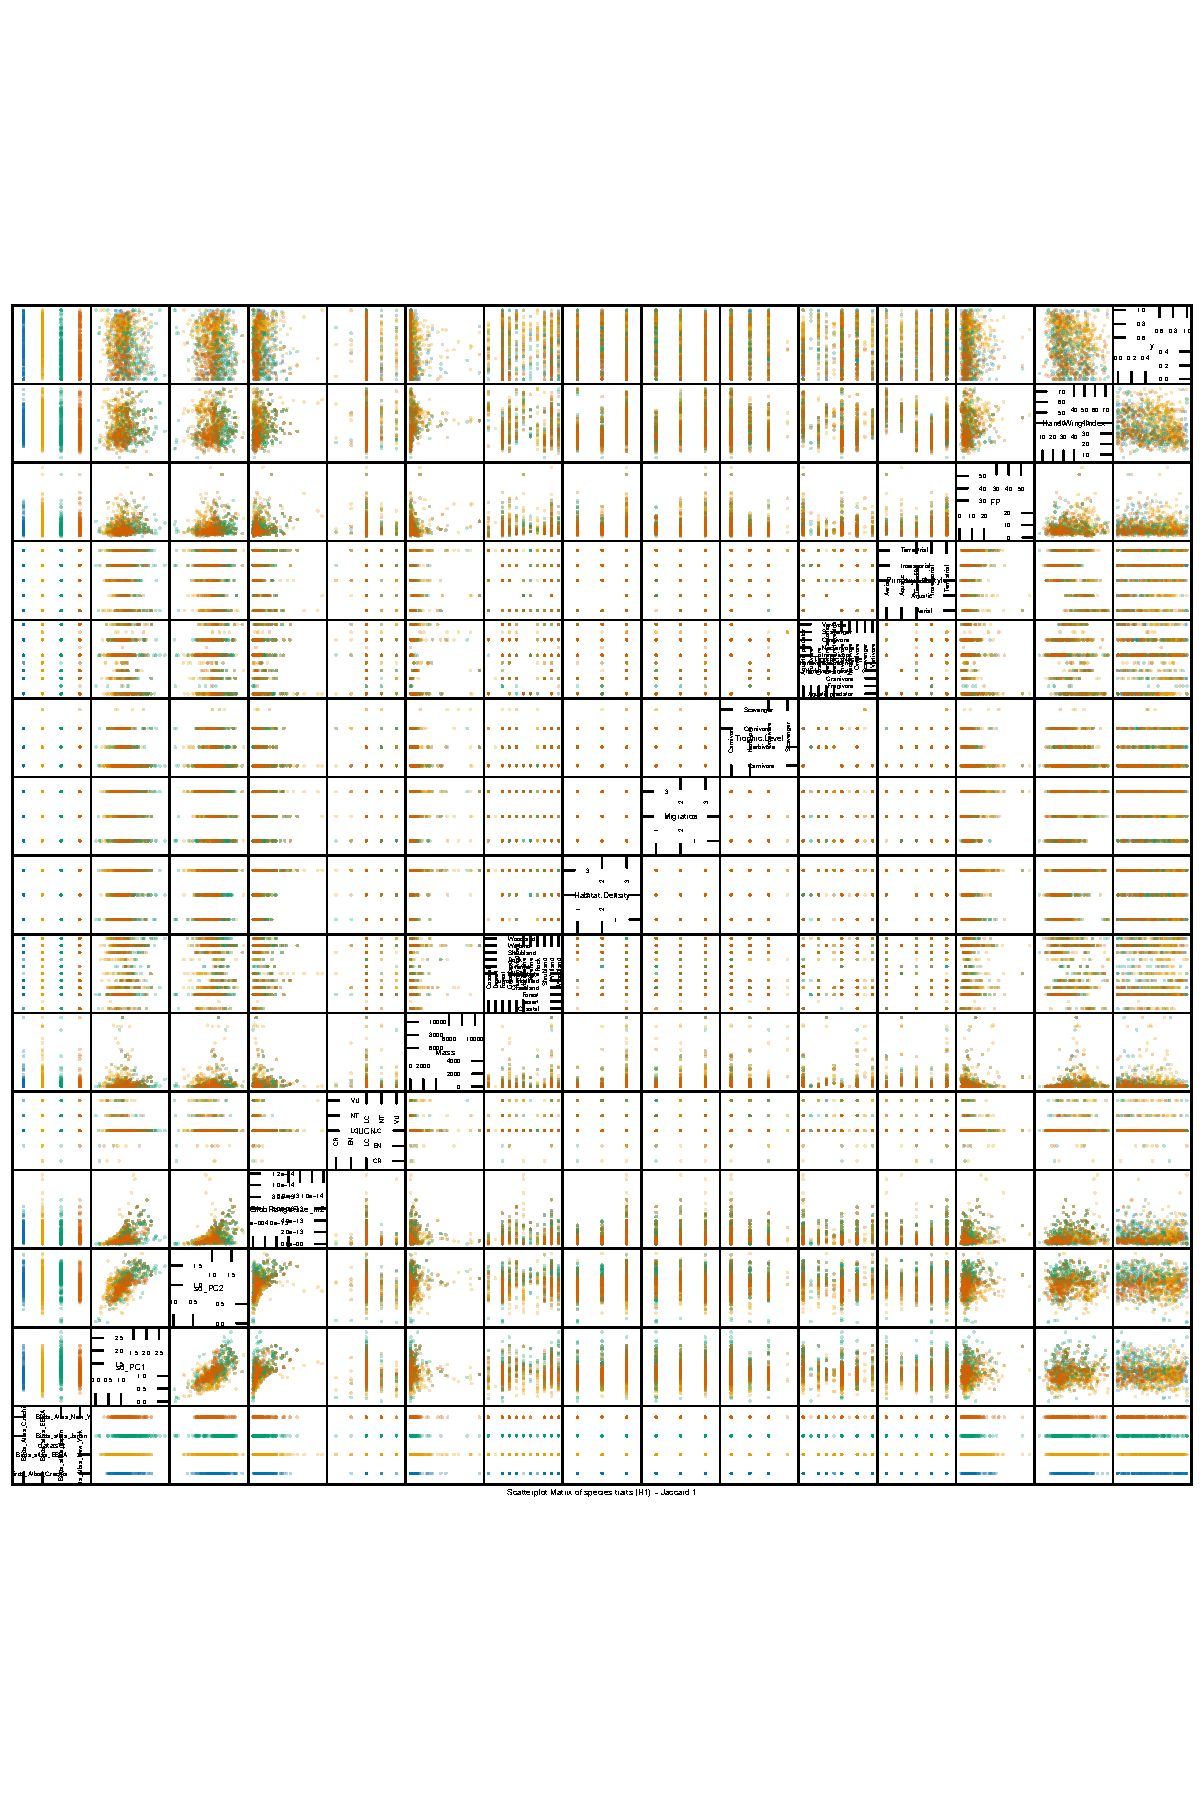
\includegraphics{01_DataPrep_files/figure-pdf/feature-plot-H1-1.pdf}

\begin{Shaded}
\begin{Highlighting}[]
\FunctionTok{featurePlot}\NormalTok{(}\AttributeTok{x =}\NormalTok{ dat\_J2 }\SpecialCharTok{\%\textgreater{}\%} \FunctionTok{select}\NormalTok{(dataset, }\FunctionTok{all\_of}\NormalTok{(H1\_vars)),}
    \AttributeTok{y =}\NormalTok{ dat\_J2}\SpecialCharTok{$}\NormalTok{Jaccard,}
    \AttributeTok{group =}\NormalTok{ dat\_J2}\SpecialCharTok{$}\NormalTok{dataset,}
    \AttributeTok{plot =} \StringTok{"pairs"}\NormalTok{,}
    \AttributeTok{pch =} \DecValTok{16}\NormalTok{,}
    \AttributeTok{alpha =} \FloatTok{0.3}\NormalTok{,}
    \AttributeTok{cex =} \FloatTok{0.2}\NormalTok{,}
    \AttributeTok{xlab =} \StringTok{"Scatterplot Matrix of species traits (H1) {-} Jaccard 2"}\NormalTok{,}
    \AttributeTok{par.settings =}
        \FunctionTok{list}\NormalTok{(}\AttributeTok{fontsize =} \FunctionTok{list}\NormalTok{(}\AttributeTok{text =} \DecValTok{4}\NormalTok{)))}
\end{Highlighting}
\end{Shaded}

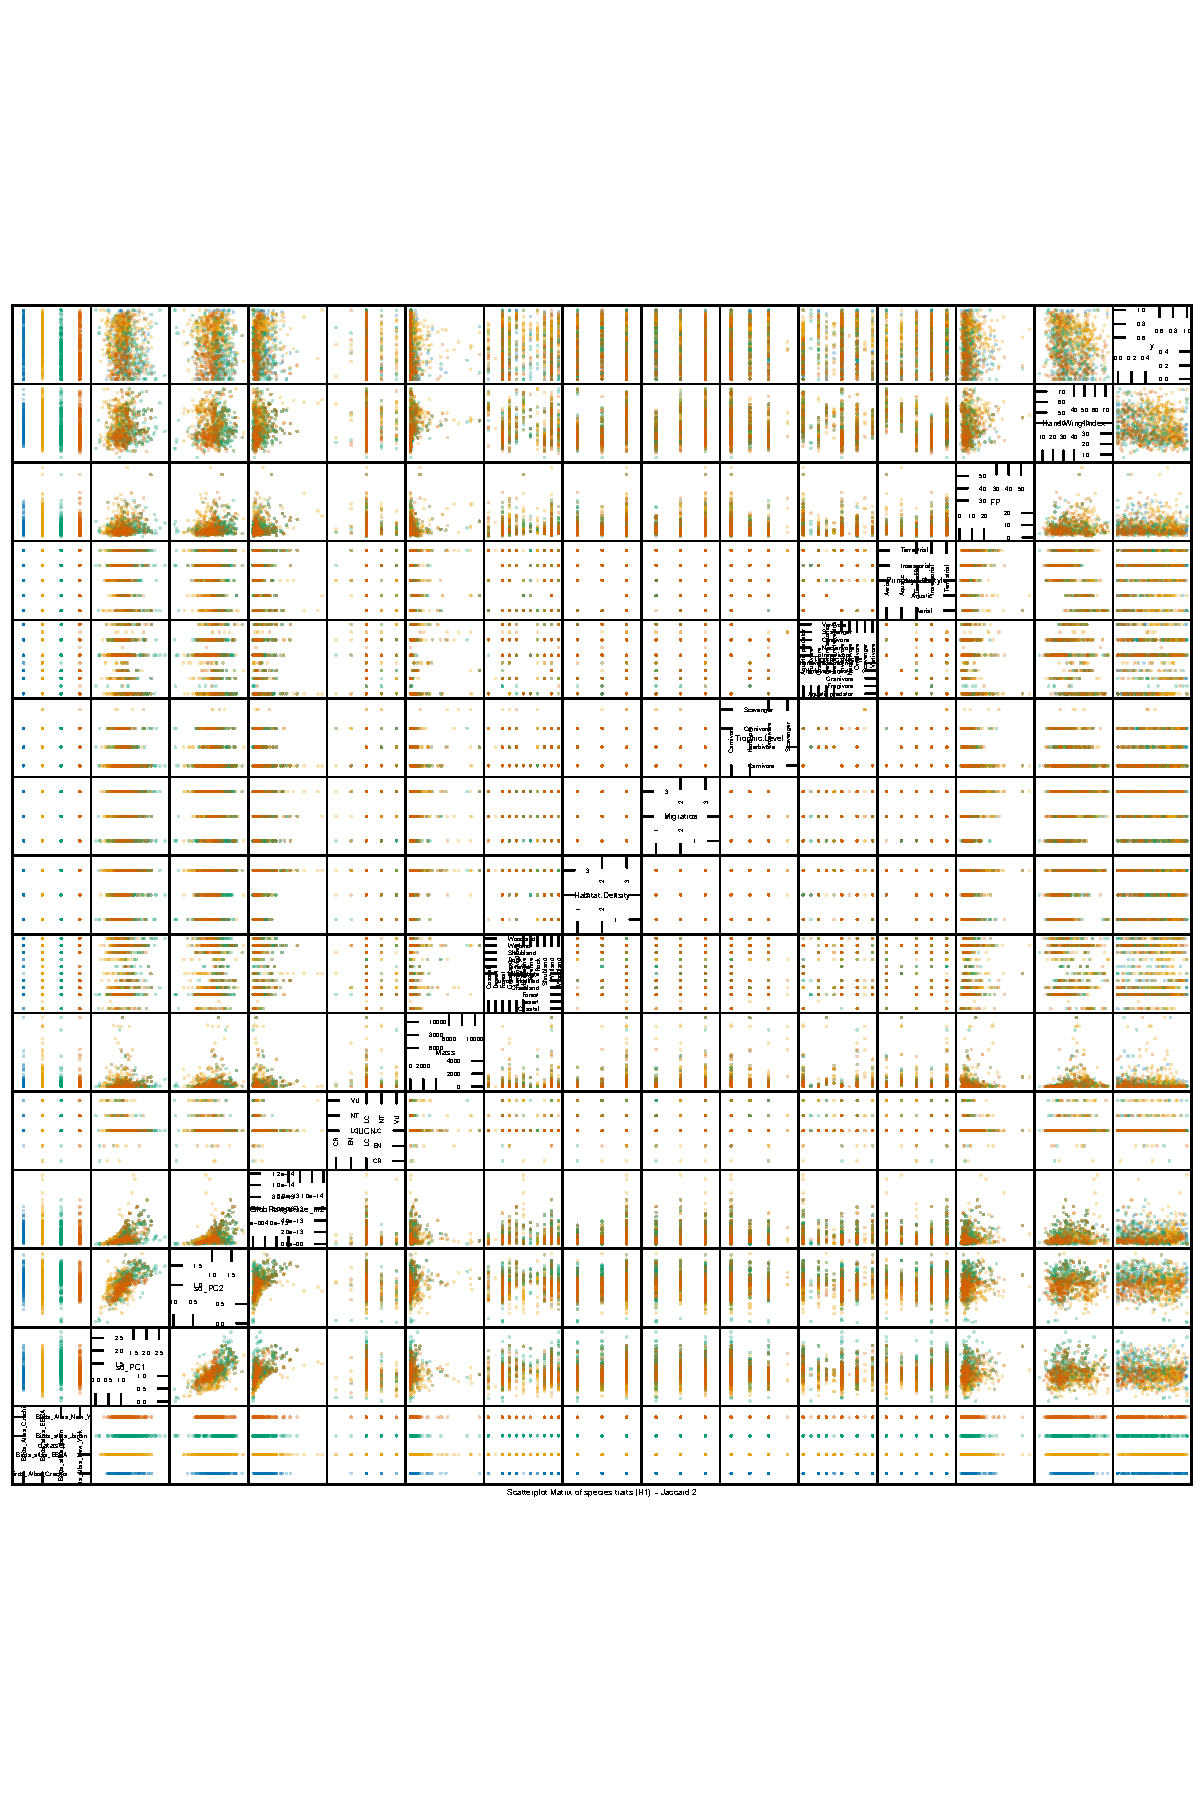
\includegraphics{01_DataPrep_files/figure-pdf/feature-plot-H1-2.pdf}

\begin{Shaded}
\begin{Highlighting}[]
\FunctionTok{featurePlot}\NormalTok{(}\AttributeTok{x =}\NormalTok{ dat\_LR1 }\SpecialCharTok{\%\textgreater{}\%} \FunctionTok{select}\NormalTok{(dataset, }\FunctionTok{all\_of}\NormalTok{(H1\_vars)),}
    \AttributeTok{y =}\NormalTok{ dat\_LR1}\SpecialCharTok{$}\NormalTok{log\_R2\_1,}
    \AttributeTok{group =}\NormalTok{ dat\_LR1}\SpecialCharTok{$}\NormalTok{dataset,}
    \AttributeTok{plot =} \StringTok{"pairs"}\NormalTok{,}
    \AttributeTok{pch =} \DecValTok{16}\NormalTok{,}
    \AttributeTok{alpha =} \FloatTok{0.3}\NormalTok{,}
    \AttributeTok{cex =} \FloatTok{0.2}\NormalTok{,}
    \AttributeTok{xlab =} \StringTok{"Scatterplot Matrix of species traits (H1) {-} Log ratio 1"}\NormalTok{,}
    \AttributeTok{par.settings =}
        \FunctionTok{list}\NormalTok{(}\AttributeTok{fontsize =} \FunctionTok{list}\NormalTok{(}\AttributeTok{text =} \DecValTok{4}\NormalTok{)))}
\end{Highlighting}
\end{Shaded}

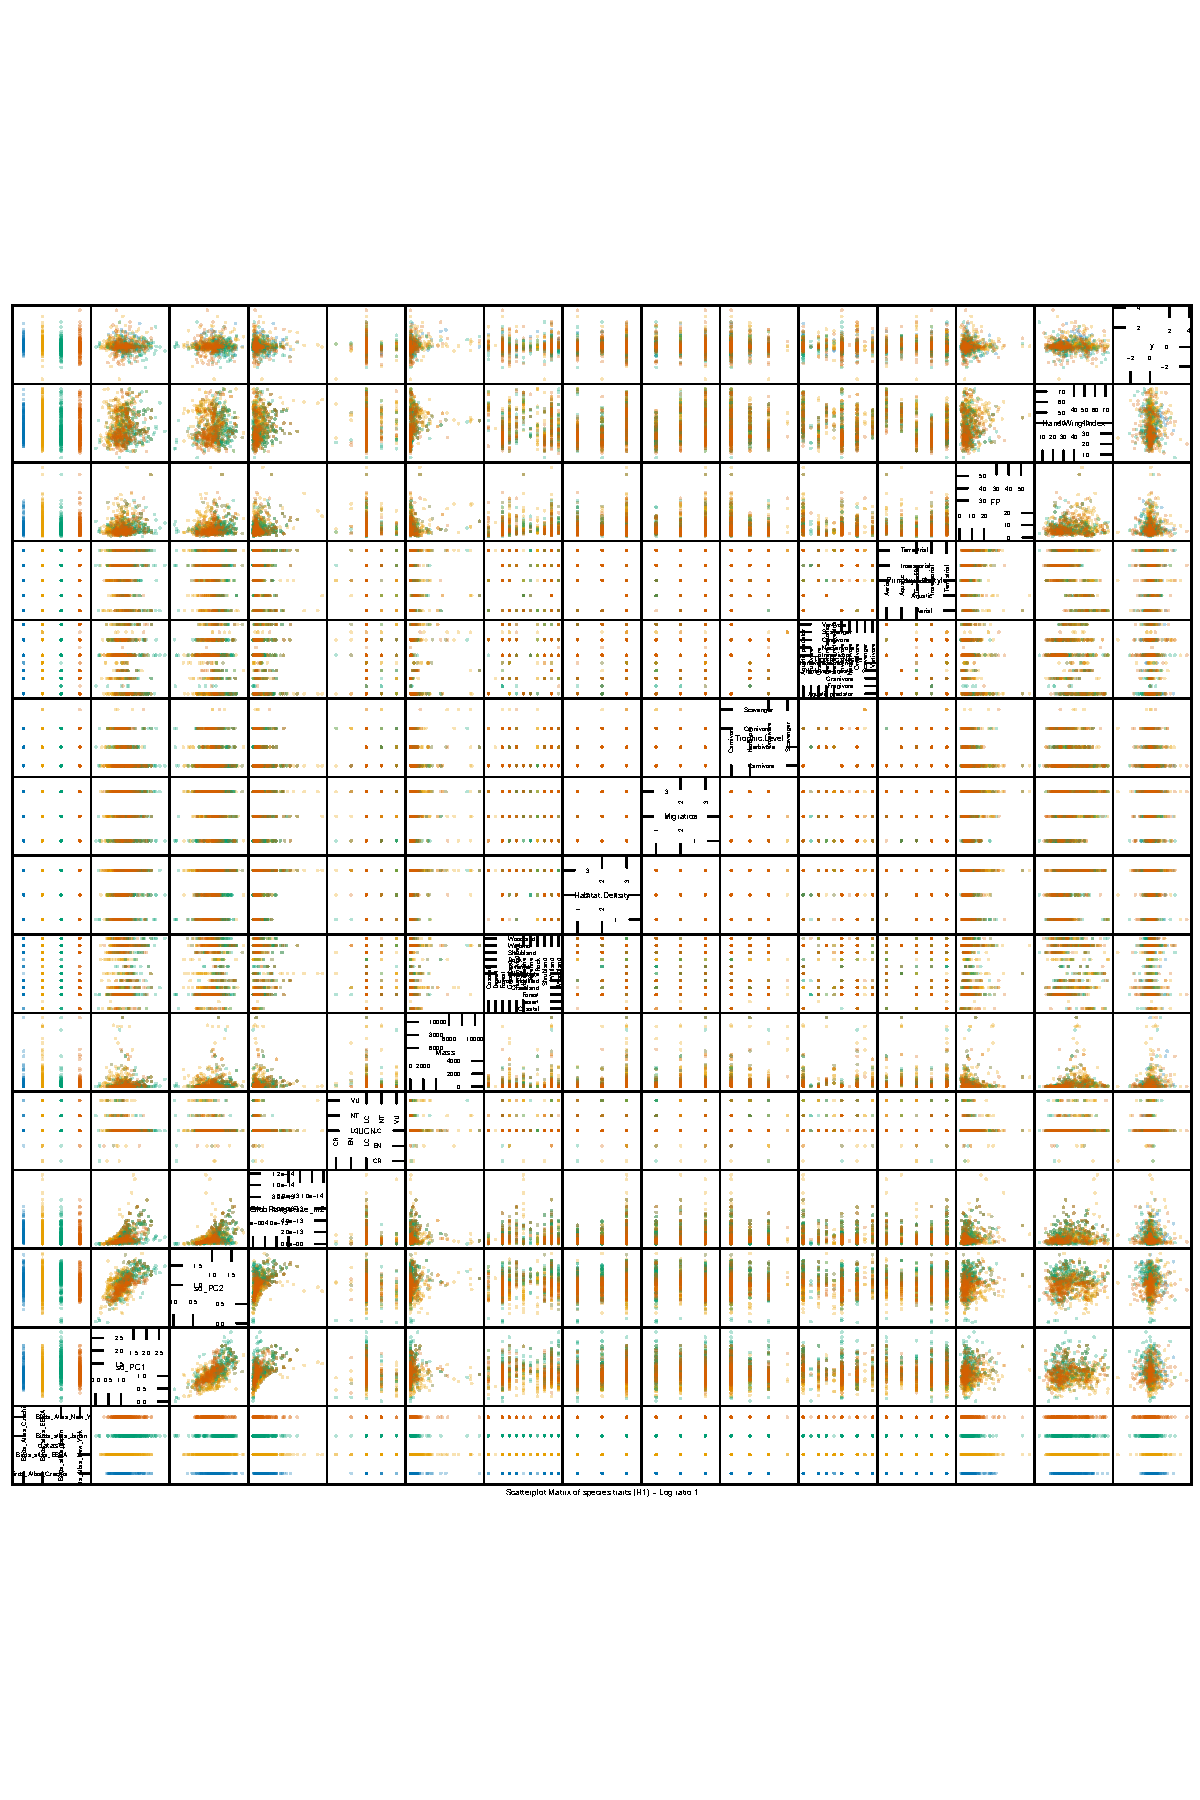
\includegraphics{01_DataPrep_files/figure-pdf/feature-plot-H1-3.pdf}

\begin{Shaded}
\begin{Highlighting}[]
\FunctionTok{featurePlot}\NormalTok{(}\AttributeTok{x =}\NormalTok{ dat\_LR2 }\SpecialCharTok{\%\textgreater{}\%} \FunctionTok{select}\NormalTok{(dataset, }\FunctionTok{all\_of}\NormalTok{(H1\_vars)),}
    \AttributeTok{y =}\NormalTok{ dat\_LR2}\SpecialCharTok{$}\NormalTok{log\_R2\_1,}
    \AttributeTok{group =}\NormalTok{ dat\_LR2}\SpecialCharTok{$}\NormalTok{dataset,}
    \AttributeTok{plot =} \StringTok{"pairs"}\NormalTok{,}
    \AttributeTok{pch =} \DecValTok{16}\NormalTok{,}
    \AttributeTok{alpha =} \FloatTok{0.3}\NormalTok{,}
    \AttributeTok{cex =} \FloatTok{0.2}\NormalTok{,}
    \AttributeTok{xlab =} \StringTok{"Scatterplot Matrix of species traits (H1) {-} log Ratio 2"}\NormalTok{,}
    \AttributeTok{par.settings =}
        \FunctionTok{list}\NormalTok{(}\AttributeTok{fontsize =} \FunctionTok{list}\NormalTok{(}\AttributeTok{text =} \DecValTok{4}\NormalTok{)))}
\end{Highlighting}
\end{Shaded}

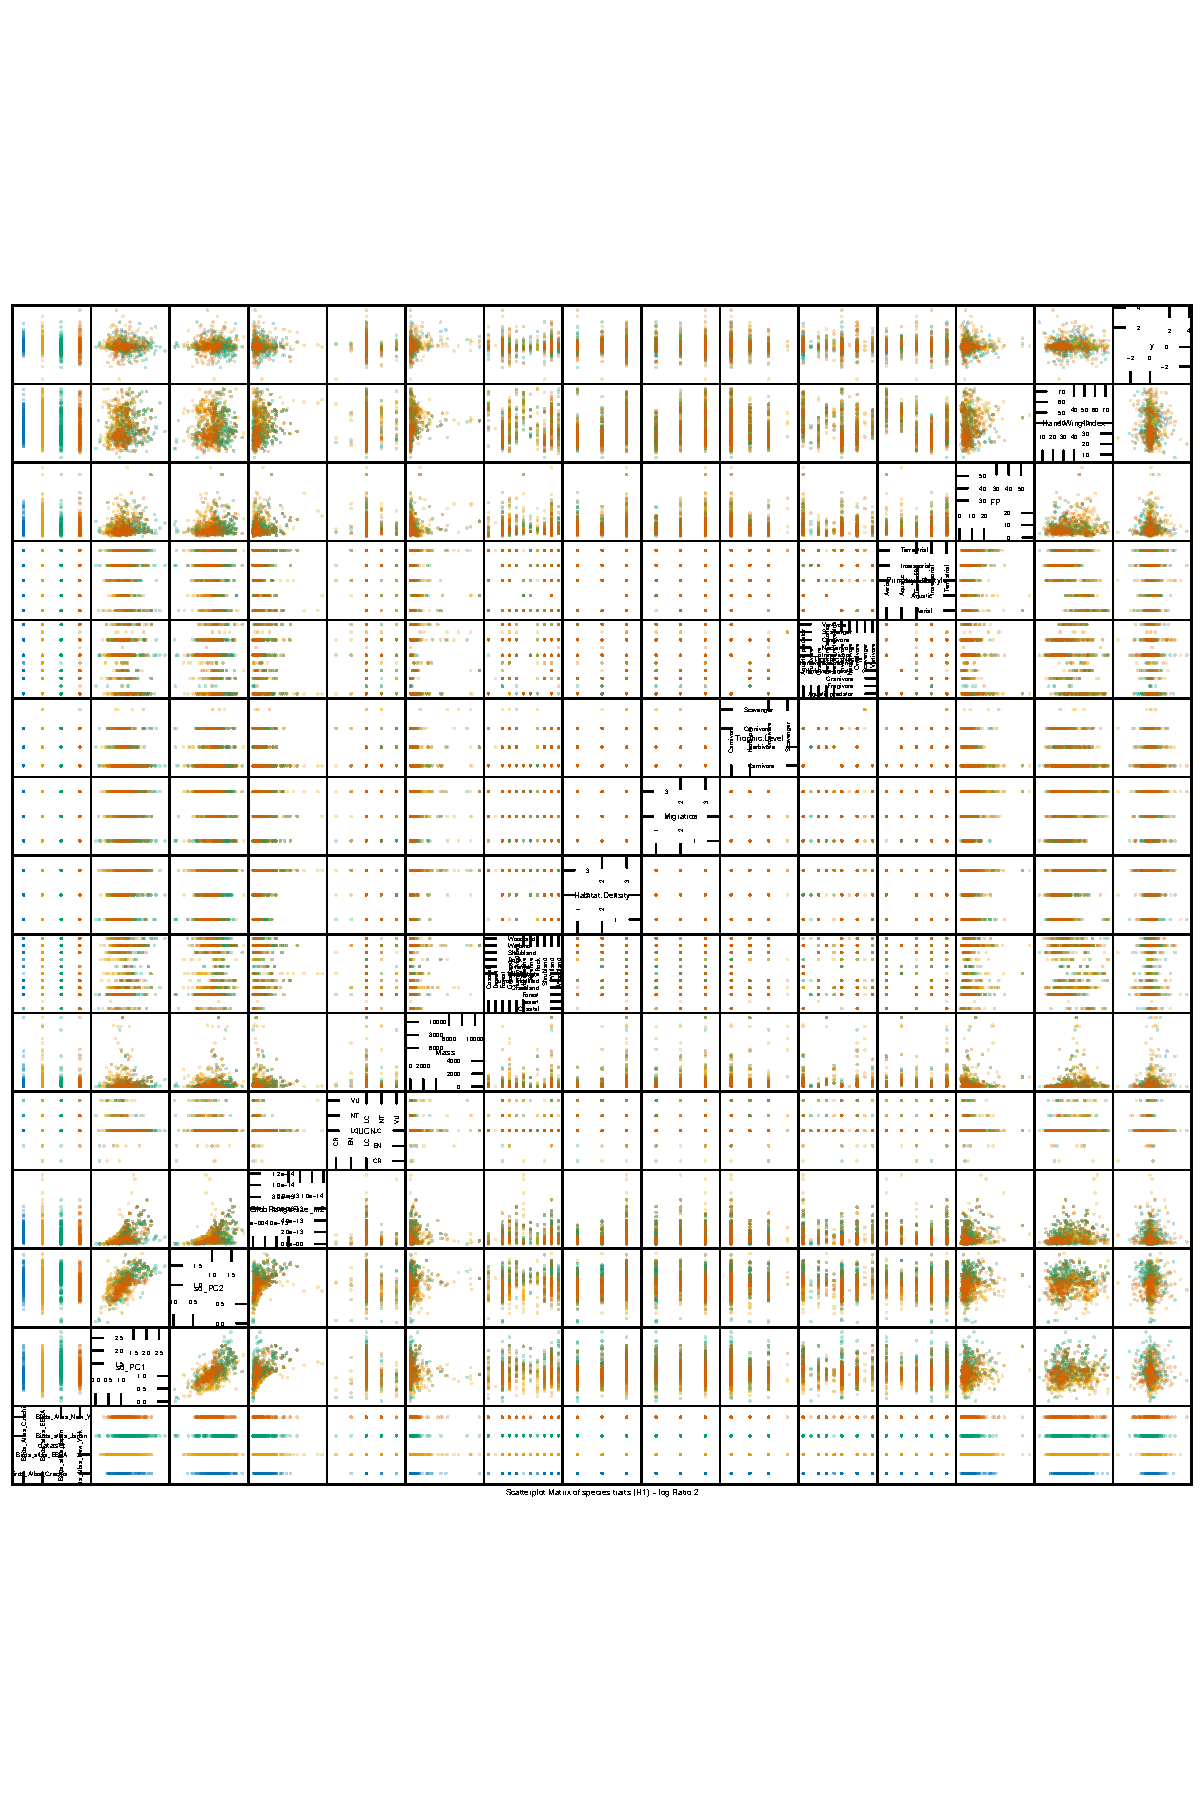
\includegraphics{01_DataPrep_files/figure-pdf/feature-plot-H1-4.pdf}

\section{Feature plot: H2}

\begin{Shaded}
\begin{Highlighting}[]
\FunctionTok{featurePlot}\NormalTok{(}\AttributeTok{x =}\NormalTok{ dat\_J1 }\SpecialCharTok{\%\textgreater{}\%} \FunctionTok{select}\NormalTok{(dataset, }\FunctionTok{all\_of}\NormalTok{(H2\_vars)),}
    \AttributeTok{y =}\NormalTok{ dat\_J1}\SpecialCharTok{$}\NormalTok{Jaccard,}
    \AttributeTok{group =}\NormalTok{ dat\_J1}\SpecialCharTok{$}\NormalTok{dataset,}
    \AttributeTok{plot =} \StringTok{"pairs"}\NormalTok{,}
    \AttributeTok{pch =} \DecValTok{16}\NormalTok{,}
    \AttributeTok{alpha =} \FloatTok{0.3}\NormalTok{,}
    \AttributeTok{cex =} \FloatTok{0.2}\NormalTok{,}
    \AttributeTok{xlab =} \StringTok{"Scatterplot Matrix of species geometry (H2) {-} Jaccard 1"}\NormalTok{,}
    \AttributeTok{par.settings =}
        \FunctionTok{list}\NormalTok{(}\AttributeTok{fontsize =} \FunctionTok{list}\NormalTok{(}\AttributeTok{text =} \DecValTok{4}\NormalTok{)))}
\end{Highlighting}
\end{Shaded}

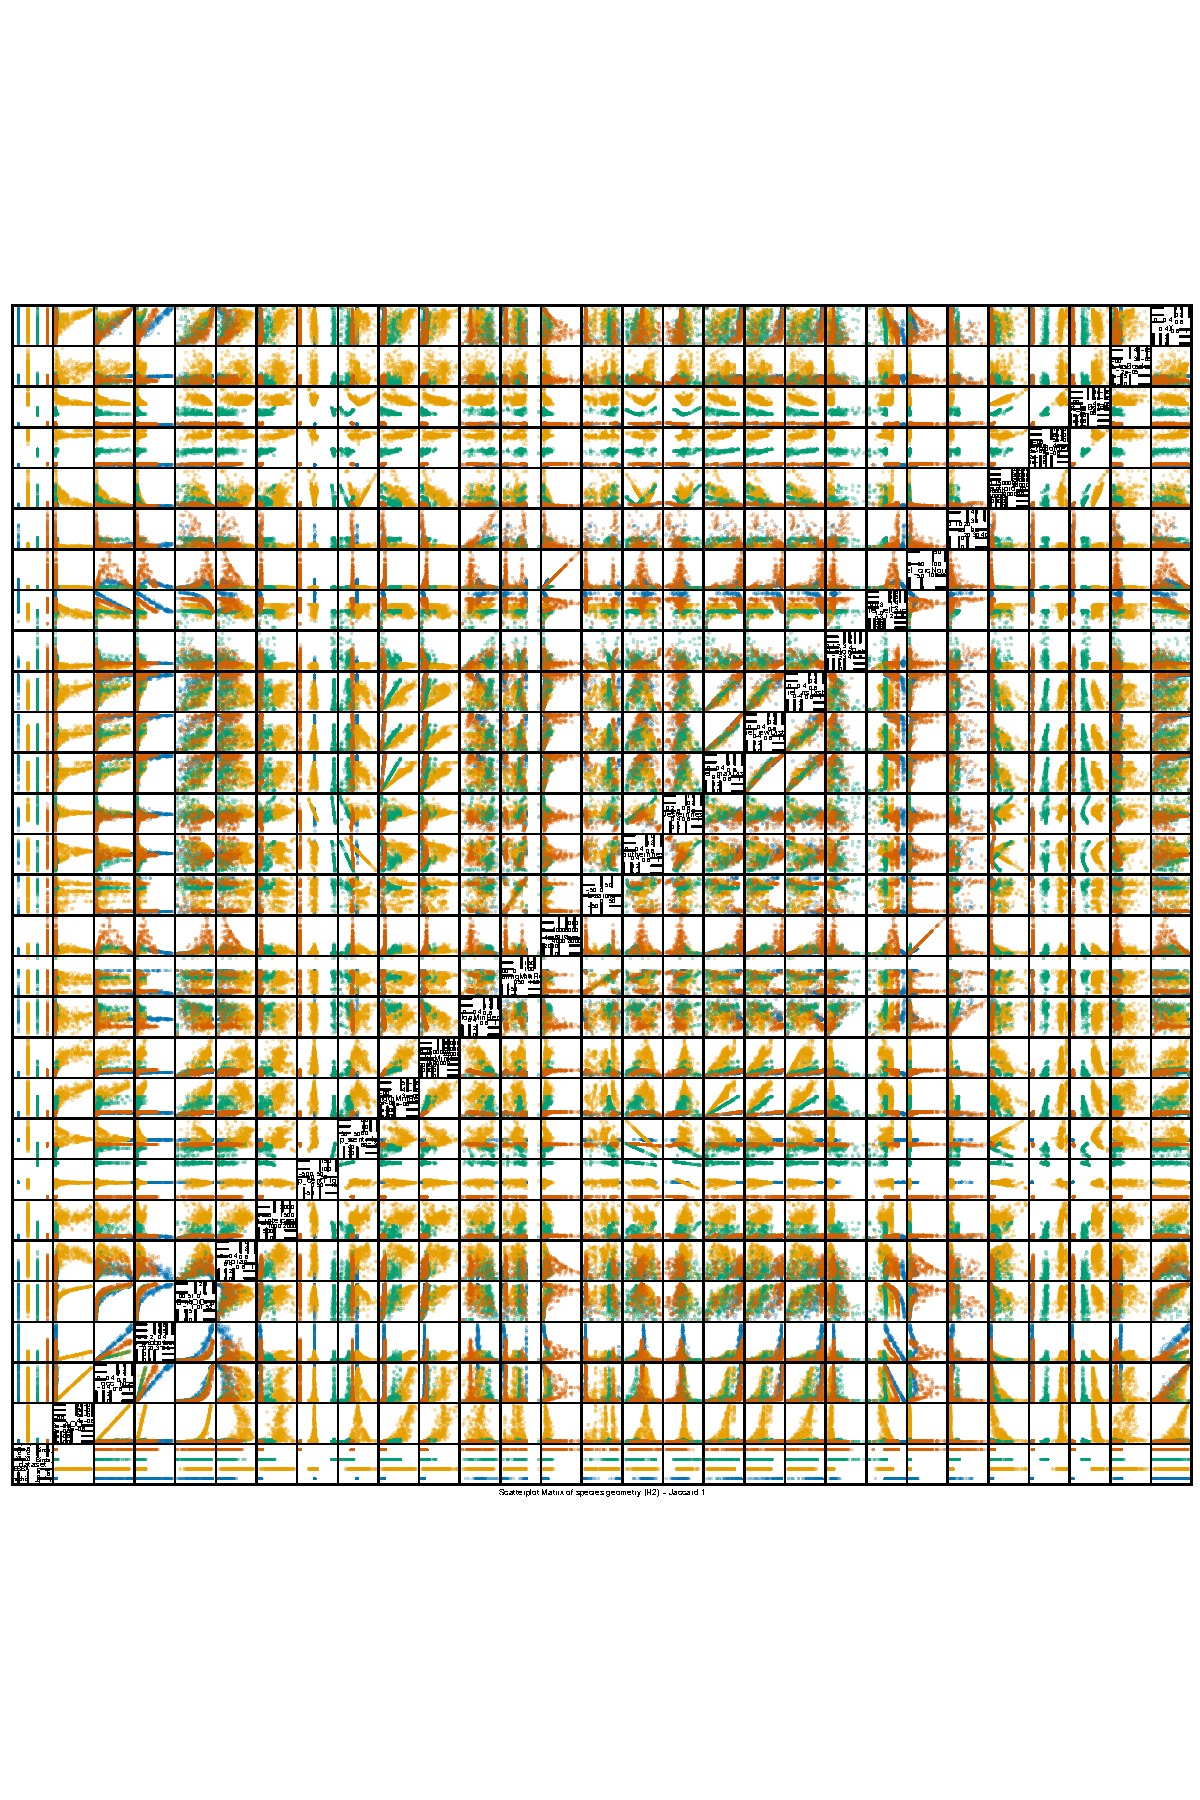
\includegraphics{01_DataPrep_files/figure-pdf/feature-plot-H2-1.pdf}

\begin{Shaded}
\begin{Highlighting}[]
\FunctionTok{featurePlot}\NormalTok{(}\AttributeTok{x =}\NormalTok{ dat\_J2 }\SpecialCharTok{\%\textgreater{}\%} \FunctionTok{select}\NormalTok{(dataset, }\FunctionTok{all\_of}\NormalTok{(H2\_vars)),}
    \AttributeTok{y =}\NormalTok{ dat\_J2}\SpecialCharTok{$}\NormalTok{Jaccard,}
    \AttributeTok{group =}\NormalTok{ dat\_J2}\SpecialCharTok{$}\NormalTok{dataset,}
    \AttributeTok{plot =} \StringTok{"pairs"}\NormalTok{,}
    \AttributeTok{pch =} \DecValTok{16}\NormalTok{,}
    \AttributeTok{alpha =} \FloatTok{0.3}\NormalTok{,}
    \AttributeTok{cex =} \FloatTok{0.2}\NormalTok{,}
    \AttributeTok{xlab =} \StringTok{"Scatterplot Matrix of species geometry (H2) {-} Jaccard 2"}\NormalTok{,}
    \AttributeTok{par.settings =}
        \FunctionTok{list}\NormalTok{(}\AttributeTok{fontsize =} \FunctionTok{list}\NormalTok{(}\AttributeTok{text =} \DecValTok{4}\NormalTok{)))}
\end{Highlighting}
\end{Shaded}

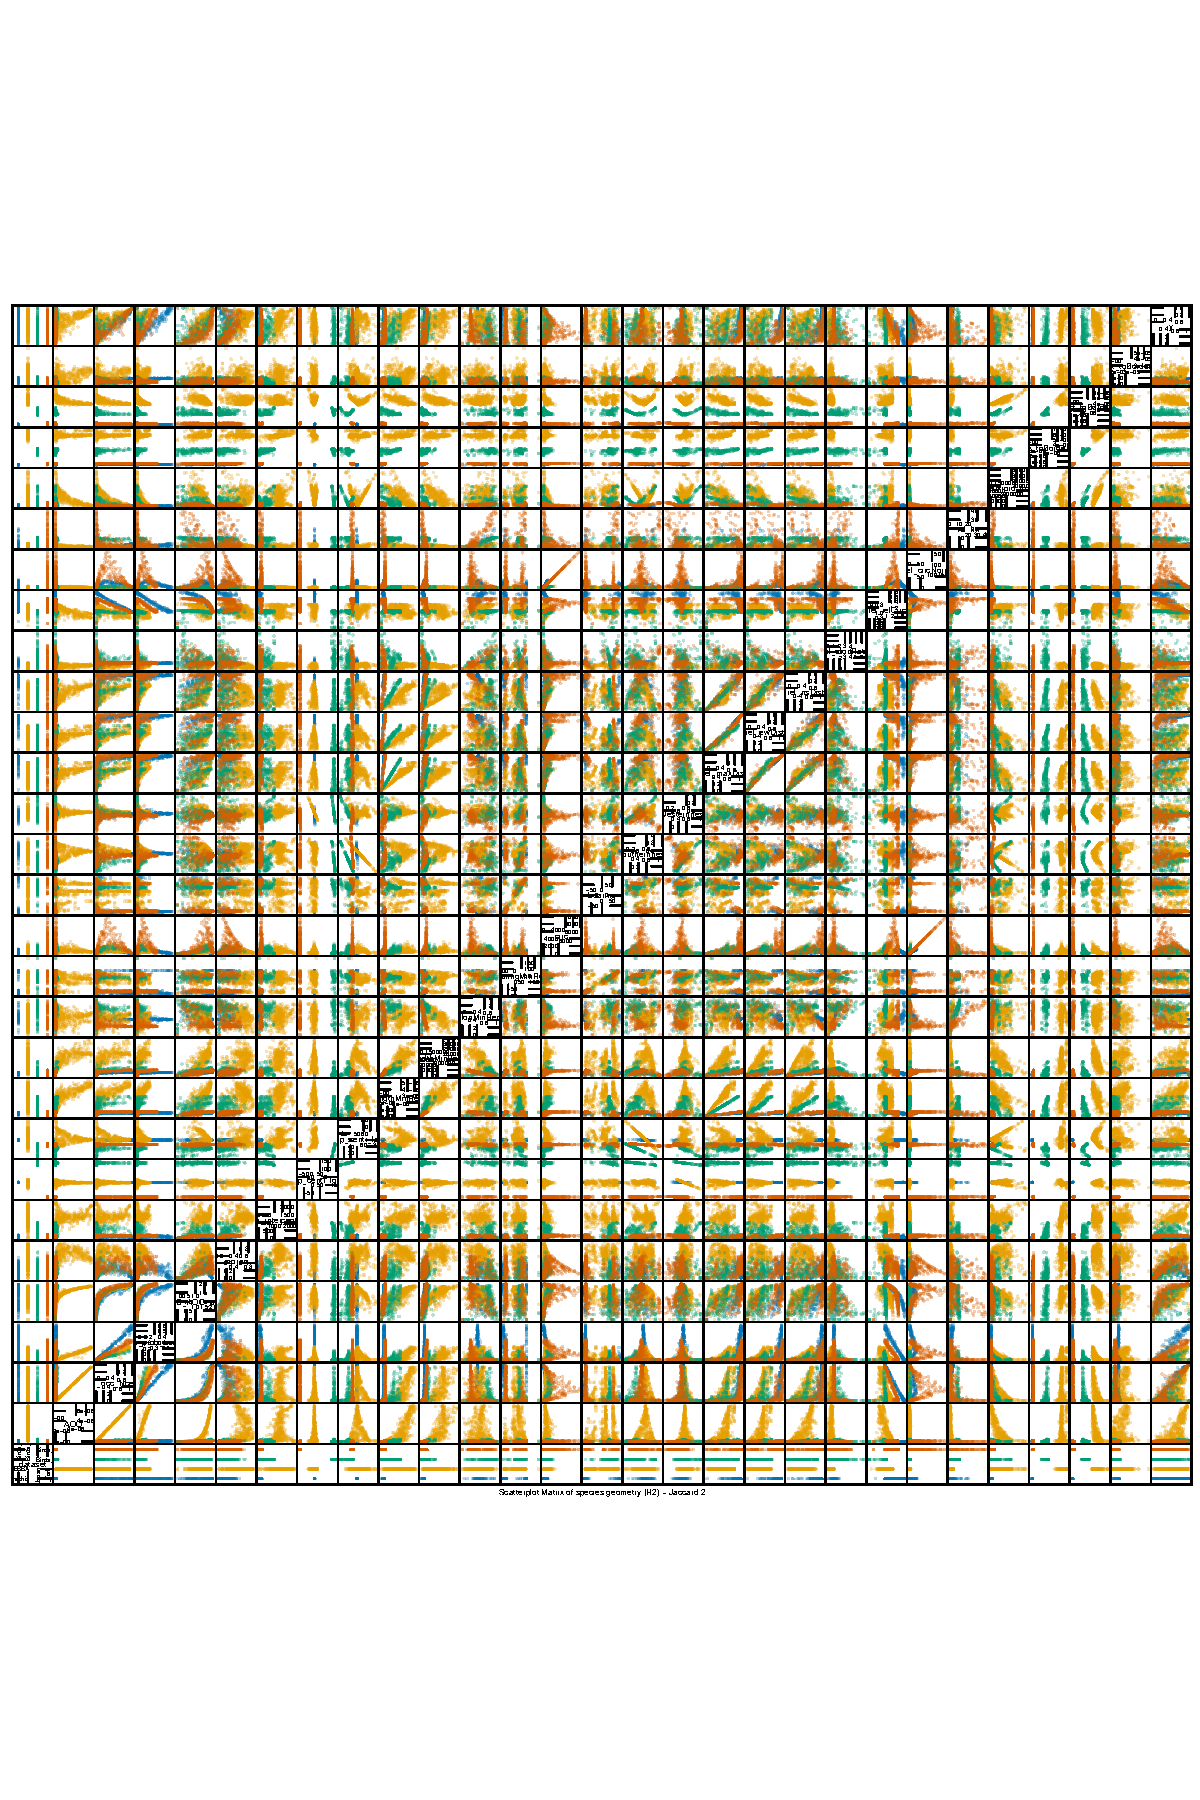
\includegraphics{01_DataPrep_files/figure-pdf/feature-plot-H2-2.pdf}

\begin{Shaded}
\begin{Highlighting}[]
\FunctionTok{featurePlot}\NormalTok{(}\AttributeTok{x =}\NormalTok{ dat\_LR1 }\SpecialCharTok{\%\textgreater{}\%} \FunctionTok{select}\NormalTok{(dataset, }\FunctionTok{all\_of}\NormalTok{(H2\_vars)),}
    \AttributeTok{y =}\NormalTok{ dat\_LR1}\SpecialCharTok{$}\NormalTok{log\_R2\_1,}
    \AttributeTok{group =}\NormalTok{ dat\_LR1}\SpecialCharTok{$}\NormalTok{dataset,}
    \AttributeTok{plot =} \StringTok{"pairs"}\NormalTok{,}
    \AttributeTok{pch =} \DecValTok{16}\NormalTok{,}
    \AttributeTok{alpha =} \FloatTok{0.3}\NormalTok{,}
    \AttributeTok{cex =} \FloatTok{0.2}\NormalTok{,}
    \AttributeTok{xlab =} \StringTok{"Scatterplot Matrix of species geometry (H2) {-} log Ratio 1"}\NormalTok{,}
    \AttributeTok{par.settings =}
        \FunctionTok{list}\NormalTok{(}\AttributeTok{fontsize =} \FunctionTok{list}\NormalTok{(}\AttributeTok{text =} \DecValTok{4}\NormalTok{)))}
\end{Highlighting}
\end{Shaded}

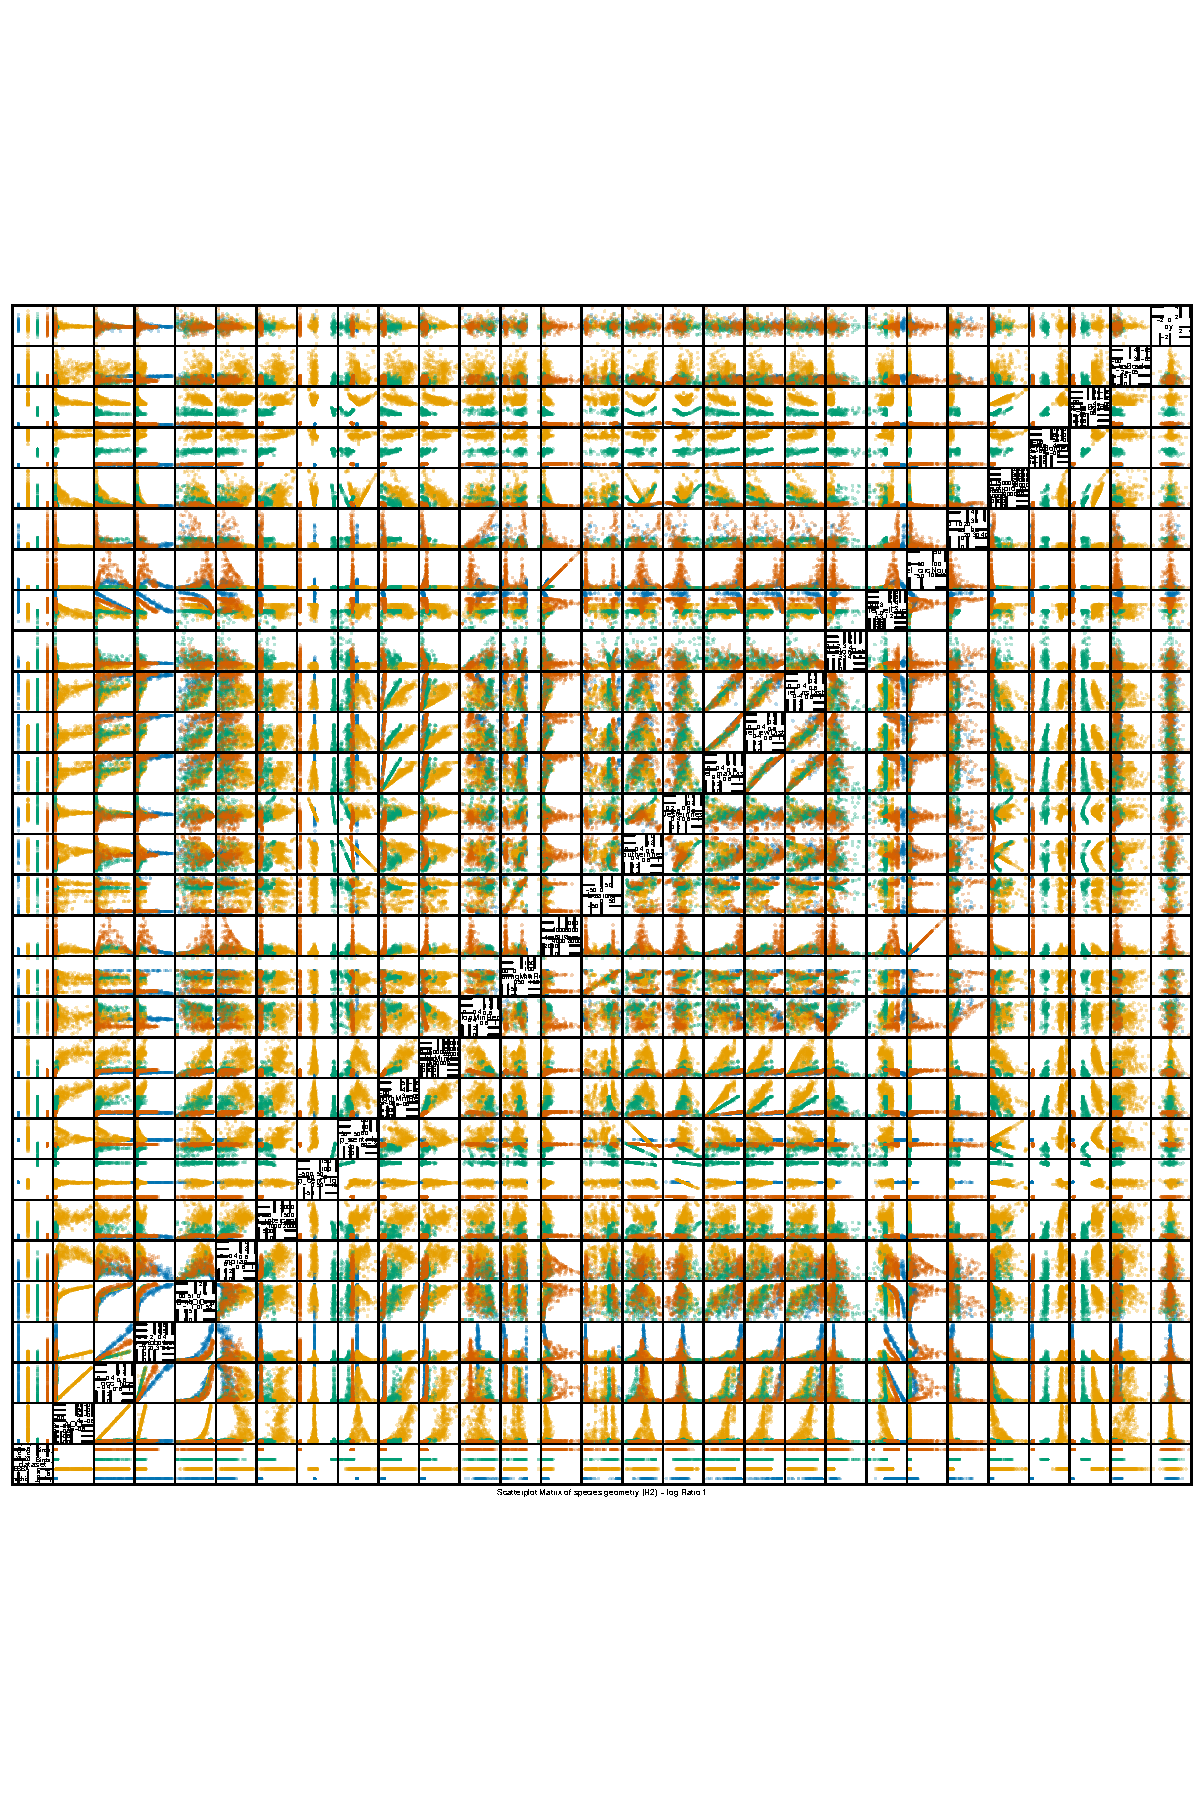
\includegraphics{01_DataPrep_files/figure-pdf/feature-plot-H2-3.pdf}

\begin{Shaded}
\begin{Highlighting}[]
\FunctionTok{featurePlot}\NormalTok{(}\AttributeTok{x =}\NormalTok{ dat\_LR2 }\SpecialCharTok{\%\textgreater{}\%} \FunctionTok{select}\NormalTok{(dataset, }\FunctionTok{all\_of}\NormalTok{(H2\_vars)),}
    \AttributeTok{y =}\NormalTok{ dat\_LR2}\SpecialCharTok{$}\NormalTok{log\_R2\_1,}
    \AttributeTok{group =}\NormalTok{ dat\_LR2}\SpecialCharTok{$}\NormalTok{dataset,}
    \AttributeTok{plot =} \StringTok{"pairs"}\NormalTok{,}
    \AttributeTok{pch =} \DecValTok{16}\NormalTok{,}
    \AttributeTok{alpha =} \FloatTok{0.3}\NormalTok{,}
    \AttributeTok{cex =} \FloatTok{0.2}\NormalTok{,}
    \AttributeTok{xlab =} \StringTok{"Scatterplot Matrix of species geometry (H2) {-} log Ratio 2"}\NormalTok{,}
    \AttributeTok{par.settings =}
        \FunctionTok{list}\NormalTok{(}\AttributeTok{fontsize =} \FunctionTok{list}\NormalTok{(}\AttributeTok{text =} \DecValTok{4}\NormalTok{)))}
\end{Highlighting}
\end{Shaded}

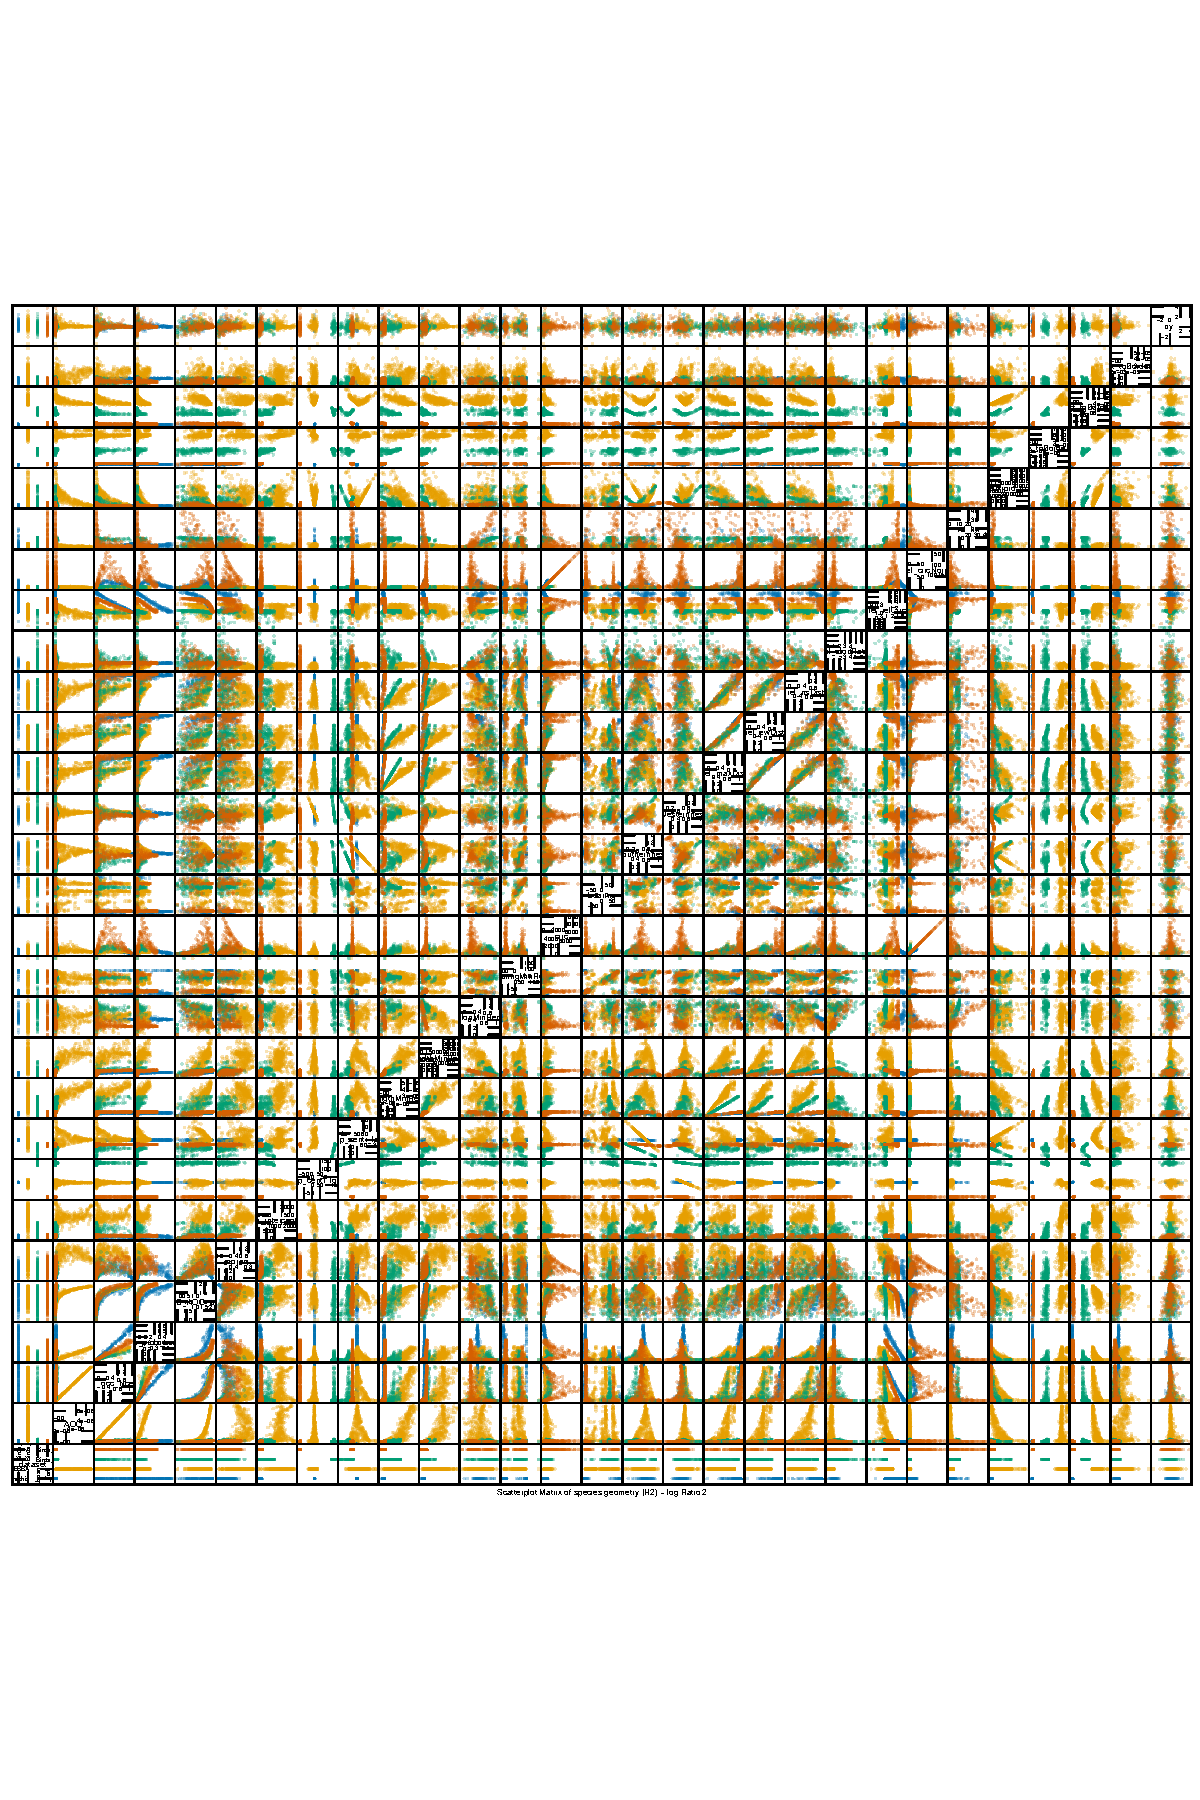
\includegraphics{01_DataPrep_files/figure-pdf/feature-plot-H2-4.pdf}

\section{Feature plot: H3}

\begin{Shaded}
\begin{Highlighting}[]
\FunctionTok{featurePlot}\NormalTok{(}\AttributeTok{x =}\NormalTok{ dat\_J1 }\SpecialCharTok{\%\textgreater{}\%} \FunctionTok{select}\NormalTok{(dataset, }\FunctionTok{all\_of}\NormalTok{(H3\_vars)),}
    \AttributeTok{y =}\NormalTok{ dat\_J1}\SpecialCharTok{$}\NormalTok{Jaccard,}
    \AttributeTok{group =}\NormalTok{ dat\_J1}\SpecialCharTok{$}\NormalTok{dataset,}
    \AttributeTok{plot =} \StringTok{"pairs"}\NormalTok{,}
    \AttributeTok{pch =} \DecValTok{16}\NormalTok{,}
    \AttributeTok{alpha =} \FloatTok{0.3}\NormalTok{,}
    \AttributeTok{cex =} \FloatTok{0.5}\NormalTok{,}
    \AttributeTok{xlab =} \StringTok{"Scatterplot Matrix of diversity metrics (H3) {-} Jaccard 1"}\NormalTok{,}
    \AttributeTok{par.settings =}
        \FunctionTok{list}\NormalTok{(}\AttributeTok{fontsize =} \FunctionTok{list}\NormalTok{(}\AttributeTok{text =} \DecValTok{6}\NormalTok{)))}
\end{Highlighting}
\end{Shaded}

\includegraphics{01_DataPrep_files/figure-pdf/feature-plot-H3-1.pdf}

\begin{Shaded}
\begin{Highlighting}[]
\FunctionTok{featurePlot}\NormalTok{(}\AttributeTok{x =}\NormalTok{ dat\_J2 }\SpecialCharTok{\%\textgreater{}\%} \FunctionTok{select}\NormalTok{(dataset, }\FunctionTok{all\_of}\NormalTok{(H3\_vars)),}
    \AttributeTok{y =}\NormalTok{ dat\_J2}\SpecialCharTok{$}\NormalTok{Jaccard,}
    \AttributeTok{group =}\NormalTok{ dat\_J2}\SpecialCharTok{$}\NormalTok{dataset,}
    \AttributeTok{plot =} \StringTok{"pairs"}\NormalTok{,}
    \AttributeTok{pch =} \DecValTok{16}\NormalTok{,}
    \AttributeTok{alpha =} \FloatTok{0.3}\NormalTok{,}
    \AttributeTok{cex =} \FloatTok{0.5}\NormalTok{,}
    \AttributeTok{xlab =} \StringTok{"Scatterplot Matrix of diversity metrics (H3) {-} Jaccard 2"}\NormalTok{,}
    \AttributeTok{par.settings =}
        \FunctionTok{list}\NormalTok{(}\AttributeTok{fontsize =} \FunctionTok{list}\NormalTok{(}\AttributeTok{text =} \DecValTok{6}\NormalTok{)))}
\end{Highlighting}
\end{Shaded}

\includegraphics{01_DataPrep_files/figure-pdf/feature-plot-H3-2.pdf}

\begin{Shaded}
\begin{Highlighting}[]
\FunctionTok{featurePlot}\NormalTok{(}\AttributeTok{x =}\NormalTok{ dat\_LR1 }\SpecialCharTok{\%\textgreater{}\%} \FunctionTok{select}\NormalTok{(dataset, }\FunctionTok{all\_of}\NormalTok{(H3\_vars)),}
    \AttributeTok{y =}\NormalTok{ dat\_LR1}\SpecialCharTok{$}\NormalTok{log\_R2\_1,}
    \AttributeTok{group =}\NormalTok{ dat\_LR1}\SpecialCharTok{$}\NormalTok{dataset,}
    \AttributeTok{plot =} \StringTok{"pairs"}\NormalTok{,}
    \AttributeTok{pch =} \DecValTok{16}\NormalTok{,}
    \AttributeTok{alpha =} \FloatTok{0.3}\NormalTok{,}
    \AttributeTok{cex =} \FloatTok{0.5}\NormalTok{,}
    \AttributeTok{xlab =} \StringTok{"Scatterplot Matrix of diversity metrics (H3) {-} log Ratio 1"}\NormalTok{,}
    \AttributeTok{par.settings =}
        \FunctionTok{list}\NormalTok{(}\AttributeTok{fontsize =} \FunctionTok{list}\NormalTok{(}\AttributeTok{text =} \DecValTok{6}\NormalTok{)))}
\end{Highlighting}
\end{Shaded}

\includegraphics{01_DataPrep_files/figure-pdf/feature-plot-H3-3.pdf}

\begin{Shaded}
\begin{Highlighting}[]
\FunctionTok{featurePlot}\NormalTok{(}\AttributeTok{x =}\NormalTok{ dat\_LR2 }\SpecialCharTok{\%\textgreater{}\%} \FunctionTok{select}\NormalTok{(dataset, }\FunctionTok{all\_of}\NormalTok{(H3\_vars)),}
    \AttributeTok{y =}\NormalTok{ dat\_LR2}\SpecialCharTok{$}\NormalTok{log\_R2\_1,}
    \AttributeTok{group =}\NormalTok{ dat\_LR2}\SpecialCharTok{$}\NormalTok{dataset,}
    \AttributeTok{plot =} \StringTok{"pairs"}\NormalTok{,}
    \AttributeTok{pch =} \DecValTok{16}\NormalTok{,}
    \AttributeTok{alpha =} \FloatTok{0.3}\NormalTok{,}
    \AttributeTok{cex =} \FloatTok{0.5}\NormalTok{,}
    \AttributeTok{xlab =} \StringTok{"Scatterplot Matrix of diversity metrics (H3) {-} log Ratio 1"}\NormalTok{,}
    \AttributeTok{par.settings =}
        \FunctionTok{list}\NormalTok{(}\AttributeTok{fontsize =} \FunctionTok{list}\NormalTok{(}\AttributeTok{text =} \DecValTok{6}\NormalTok{)))}
\end{Highlighting}
\end{Shaded}

\includegraphics{01_DataPrep_files/figure-pdf/feature-plot-H3-4.pdf}

\section{Feature plot: H4}

\begin{Shaded}
\begin{Highlighting}[]
\FunctionTok{featurePlot}\NormalTok{(}\AttributeTok{x =}\NormalTok{ dat\_J1 }\SpecialCharTok{\%\textgreater{}\%} \FunctionTok{select}\NormalTok{(dataset, }\FunctionTok{all\_of}\NormalTok{(H4\_vars)),}
    \AttributeTok{y =}\NormalTok{ dat\_J1}\SpecialCharTok{$}\NormalTok{Jaccard,}
    \AttributeTok{group =}\NormalTok{ dat\_J1}\SpecialCharTok{$}\NormalTok{dataset,}
    \AttributeTok{plot =} \StringTok{"pairs"}\NormalTok{,}
    \AttributeTok{pch =} \DecValTok{16}\NormalTok{,}
    \AttributeTok{alpha =} \FloatTok{0.6}\NormalTok{,}
    \AttributeTok{cex =} \FloatTok{0.5}\NormalTok{,}
    \AttributeTok{xlab =} \StringTok{"Scatterplot Matrix of atlas specifics (H4) {-} Jaccard 2"}\NormalTok{,}
    \AttributeTok{par.settings =}
        \FunctionTok{list}\NormalTok{(}\AttributeTok{fontsize =} \FunctionTok{list}\NormalTok{(}\AttributeTok{text =} \DecValTok{5}\NormalTok{)))}
\end{Highlighting}
\end{Shaded}

\includegraphics{01_DataPrep_files/figure-pdf/feature-plot-H4-1.pdf}

\begin{Shaded}
\begin{Highlighting}[]
\FunctionTok{featurePlot}\NormalTok{(}\AttributeTok{x =}\NormalTok{ dat\_J2 }\SpecialCharTok{\%\textgreater{}\%} \FunctionTok{select}\NormalTok{(dataset, }\FunctionTok{all\_of}\NormalTok{(H4\_vars)),}
    \AttributeTok{y =}\NormalTok{ dat\_J2}\SpecialCharTok{$}\NormalTok{Jaccard,}
    \AttributeTok{group =}\NormalTok{ dat\_J2}\SpecialCharTok{$}\NormalTok{dataset,}
    \AttributeTok{plot =} \StringTok{"pairs"}\NormalTok{,}
    \AttributeTok{pch =} \DecValTok{16}\NormalTok{,}
    \AttributeTok{alpha =} \FloatTok{0.6}\NormalTok{,}
    \AttributeTok{cex =} \FloatTok{0.5}\NormalTok{,}
    \AttributeTok{xlab =} \StringTok{"Scatterplot Matrix of atlas specifics (H4) {-} Jaccard 2"}\NormalTok{,}
    \AttributeTok{par.settings =}
        \FunctionTok{list}\NormalTok{(}\AttributeTok{fontsize =} \FunctionTok{list}\NormalTok{(}\AttributeTok{text =} \DecValTok{5}\NormalTok{)))}
\end{Highlighting}
\end{Shaded}

\includegraphics{01_DataPrep_files/figure-pdf/feature-plot-H4-2.pdf}

\begin{Shaded}
\begin{Highlighting}[]
\FunctionTok{featurePlot}\NormalTok{(}\AttributeTok{x =}\NormalTok{ dat\_LR1 }\SpecialCharTok{\%\textgreater{}\%} \FunctionTok{select}\NormalTok{(dataset, }\FunctionTok{all\_of}\NormalTok{(H4\_vars)),}
    \AttributeTok{y =}\NormalTok{ dat\_LR1}\SpecialCharTok{$}\NormalTok{log\_R2\_1,}
    \AttributeTok{group =}\NormalTok{ dat\_LR1}\SpecialCharTok{$}\NormalTok{dataset,}
    \AttributeTok{plot =} \StringTok{"pairs"}\NormalTok{,}
    \AttributeTok{pch =} \DecValTok{16}\NormalTok{,}
    \AttributeTok{alpha =} \FloatTok{0.6}\NormalTok{,}
    \AttributeTok{cex =} \FloatTok{0.5}\NormalTok{,}
    \AttributeTok{xlab =} \StringTok{"Scatterplot Matrix of atlas specifics (H4) {-} log Ratio 1"}\NormalTok{,}
    \AttributeTok{par.settings =}
        \FunctionTok{list}\NormalTok{(}\AttributeTok{fontsize =} \FunctionTok{list}\NormalTok{(}\AttributeTok{text =} \DecValTok{5}\NormalTok{)))}
\end{Highlighting}
\end{Shaded}

\includegraphics{01_DataPrep_files/figure-pdf/feature-plot-H4-3.pdf}

\begin{Shaded}
\begin{Highlighting}[]
\FunctionTok{featurePlot}\NormalTok{(}\AttributeTok{x =}\NormalTok{ dat\_LR2 }\SpecialCharTok{\%\textgreater{}\%} \FunctionTok{select}\NormalTok{(dataset, }\FunctionTok{all\_of}\NormalTok{(H4\_vars)),}
    \AttributeTok{y =}\NormalTok{ dat\_LR2}\SpecialCharTok{$}\NormalTok{log\_R2\_1,}
    \AttributeTok{group =}\NormalTok{ dat\_LR2}\SpecialCharTok{$}\NormalTok{dataset,}
    \AttributeTok{plot =} \StringTok{"pairs"}\NormalTok{,}
    \AttributeTok{pch =} \DecValTok{16}\NormalTok{,}
    \AttributeTok{alpha =} \FloatTok{0.6}\NormalTok{,}
    \AttributeTok{cex =} \FloatTok{0.5}\NormalTok{,}
    \AttributeTok{xlab =} \StringTok{"Scatterplot Matrix of atlas specifics (H4) {-} log Ratio 2"}\NormalTok{,}
    \AttributeTok{par.settings =}
        \FunctionTok{list}\NormalTok{(}\AttributeTok{fontsize =} \FunctionTok{list}\NormalTok{(}\AttributeTok{text =} \DecValTok{5}\NormalTok{)))}
\end{Highlighting}
\end{Shaded}

\includegraphics{01_DataPrep_files/figure-pdf/feature-plot-H4-4.pdf}

\section{Correlation Matrix}\label{correlation-matrix}

Next, we will check how correlated the predictors are. Those will be
automatically excluded using recipes below in: \emph{Model fitting
\textgreater{} Data pre-processing}

\begin{itemize}
\tightlist
\item
  Sampling periods 1: 17 correlated variables
\item
  Sampling periods 2: 18 correlated variables
\end{itemize}

\section{Predictor correlations for Sampling Period 1}

\begin{Shaded}
\begin{Highlighting}[]
\NormalTok{cor\_df }\OtherTok{\textless{}{-}}\NormalTok{ dat\_J1 }\SpecialCharTok{\%\textgreater{}\%} \FunctionTok{select}\NormalTok{(}\SpecialCharTok{{-}}\NormalTok{Jaccard) }\CommentTok{\# does not matter which tp = 1 data we look at}
\NormalTok{p.mat }\OtherTok{\textless{}{-}} \FunctionTok{model.matrix}\NormalTok{(}\SpecialCharTok{\textasciitilde{}} \DecValTok{0} \SpecialCharTok{+}\NormalTok{ ., }\AttributeTok{data =}\NormalTok{ cor\_df) }\SpecialCharTok{\%\textgreater{}\%}
    \FunctionTok{cor\_pmat}\NormalTok{()}

\NormalTok{correlation\_matrix }\OtherTok{\textless{}{-}}\NormalTok{ cor\_df }\SpecialCharTok{\%\textgreater{}\%}
    \FunctionTok{select\_if}\NormalTok{(is.numeric) }\SpecialCharTok{\%\textgreater{}\%}
    \FunctionTok{cor}\NormalTok{(}\AttributeTok{use =} \StringTok{"pairwise.complete.obs"}\NormalTok{)}
\NormalTok{correlation\_matrix }\SpecialCharTok{\%\textgreater{}\%}
    \FunctionTok{ggcorrplot}\NormalTok{(}
        \AttributeTok{hc.order =} \ConstantTok{TRUE}\NormalTok{,}
        \AttributeTok{lab =} \ConstantTok{TRUE}\NormalTok{,}
        \AttributeTok{lab\_size =} \DecValTok{3}\NormalTok{,}
        \AttributeTok{p.mat =}\NormalTok{ p.mat,}
        \AttributeTok{insig =} \StringTok{"blank"}
\NormalTok{    )}
\end{Highlighting}
\end{Shaded}

\includegraphics{01_DataPrep_files/figure-pdf/correlation-matrix-J1-1.pdf}

\begin{Shaded}
\begin{Highlighting}[]
\CommentTok{\# We will set the threshold for excluding correlations = 0.85}
\CommentTok{\# this is a bit arbitrary, trying to find a good trade{-}off between loss of predictor variables and collinearity}

\NormalTok{cor\_vars }\OtherTok{\textless{}{-}} \FunctionTok{findCorrelation}\NormalTok{(correlation\_matrix,}
    \AttributeTok{cutoff =}\NormalTok{ .}\DecValTok{85}\NormalTok{,}
    \AttributeTok{names =} \ConstantTok{TRUE}\NormalTok{,}
    \AttributeTok{exact =} \ConstantTok{TRUE}\NormalTok{,}
    \AttributeTok{verbose =} \ConstantTok{FALSE}\NormalTok{)}

\CommentTok{\# cor\_vars \# 17 variables seemed to be highly correlated. We will exclude}
\end{Highlighting}
\end{Shaded}

\section{Predictor correlations of Sampling period 2}

\begin{Shaded}
\begin{Highlighting}[]
\NormalTok{cor\_df }\OtherTok{\textless{}{-}}\NormalTok{ dat\_J2 }\SpecialCharTok{\%\textgreater{}\%} \FunctionTok{select}\NormalTok{(}\SpecialCharTok{{-}}\NormalTok{Jaccard)}
\NormalTok{p.mat }\OtherTok{\textless{}{-}} \FunctionTok{model.matrix}\NormalTok{(}\SpecialCharTok{\textasciitilde{}} \DecValTok{0} \SpecialCharTok{+}\NormalTok{ ., }\AttributeTok{data =}\NormalTok{ cor\_df) }\SpecialCharTok{\%\textgreater{}\%}
    \FunctionTok{cor\_pmat}\NormalTok{()}

\NormalTok{correlation\_matrix }\OtherTok{\textless{}{-}}\NormalTok{ cor\_df }\SpecialCharTok{\%\textgreater{}\%}
    \FunctionTok{select\_if}\NormalTok{(is.numeric) }\SpecialCharTok{\%\textgreater{}\%}
    \FunctionTok{cor}\NormalTok{(}\AttributeTok{use =} \StringTok{"pairwise.complete.obs"}\NormalTok{)}
\NormalTok{correlation\_matrix }\SpecialCharTok{\%\textgreater{}\%}
    \FunctionTok{ggcorrplot}\NormalTok{(}
        \AttributeTok{hc.order =} \ConstantTok{TRUE}\NormalTok{,}
        \AttributeTok{lab =} \ConstantTok{TRUE}\NormalTok{,}
        \AttributeTok{lab\_size =} \DecValTok{3}\NormalTok{,}
        \AttributeTok{p.mat =}\NormalTok{ p.mat,}
        \AttributeTok{insig =} \StringTok{"blank"}
\NormalTok{    )}
\end{Highlighting}
\end{Shaded}

\includegraphics{01_DataPrep_files/figure-pdf/correlation-matrix-J2-1.pdf}

\begin{Shaded}
\begin{Highlighting}[]
\CommentTok{\# We will set the threshold for excluding correlations = 0.85}
\CommentTok{\# this is a bit arbitrary, trying to find a good trade{-}off between loss of predictor variables and collinearity}

\NormalTok{cor\_vars }\OtherTok{\textless{}{-}} \FunctionTok{findCorrelation}\NormalTok{(correlation\_matrix,}
    \AttributeTok{cutoff =}\NormalTok{ .}\DecValTok{85}\NormalTok{,}
    \AttributeTok{names =} \ConstantTok{TRUE}\NormalTok{,}
    \AttributeTok{exact =} \ConstantTok{TRUE}\NormalTok{,}
    \AttributeTok{verbose =} \ConstantTok{FALSE}\NormalTok{)}

\CommentTok{\# cor\_vars \# 18 variables seemed to be highly correlated. We will exclude}
\end{Highlighting}
\end{Shaded}

\bookmarksetup{startatroot}

\chapter{Model fitting}\label{model-fitting}

We will be using the following models for comparative reasons:

\begin{enumerate}
\def\labelenumi{\arabic{enumi}.}
\tightlist
\item
  Random Forest (\texttt{ranger})
\item
  Extreme Gradient Boosting (\texttt{xgboost})
\item
  Boosted Regression trees (\texttt{gbm})
\end{enumerate}

In addition, we will fit an ensemble model and compare it's predictive
performance to the individual models. All of this can be done in
\texttt{caret} and \texttt{caretEnsemble.}

\subsection{Data pre-processing:}\label{data-pre-processing}

\begin{itemize}
\tightlist
\item
  First we have to check if there are (near) zero variance variables in
  the predictors. These can be removed since they will not explain a lot
  generally.
\end{itemize}

\begin{Shaded}
\begin{Highlighting}[]
\CommentTok{\# Step 1. Near Zero Vars}
\FunctionTok{rbind}\NormalTok{(}
\FunctionTok{nearZeroVar}\NormalTok{(dat\_J1, }\AttributeTok{saveMetrics =}\NormalTok{ T) }\SpecialCharTok{\%\textgreater{}\%} \FunctionTok{filter}\NormalTok{(nzv }\SpecialCharTok{==}\NormalTok{ T),}
\FunctionTok{nearZeroVar}\NormalTok{(dat\_J2, }\AttributeTok{saveMetrics =}\NormalTok{ T) }\SpecialCharTok{\%\textgreater{}\%} \FunctionTok{filter}\NormalTok{(nzv }\SpecialCharTok{==}\NormalTok{ T),}
\FunctionTok{nearZeroVar}\NormalTok{(dat\_LR1, }\AttributeTok{saveMetrics =}\NormalTok{ T) }\SpecialCharTok{\%\textgreater{}\%} \FunctionTok{filter}\NormalTok{(nzv }\SpecialCharTok{==}\NormalTok{ T),}
\FunctionTok{nearZeroVar}\NormalTok{(dat\_LR2, }\AttributeTok{saveMetrics =}\NormalTok{ T) }\SpecialCharTok{\%\textgreater{}\%} \FunctionTok{filter}\NormalTok{(nzv }\SpecialCharTok{==}\NormalTok{ T)) }\SpecialCharTok{\%\textgreater{}\%} 
\NormalTok{  kableExtra}\SpecialCharTok{::}\FunctionTok{kable}\NormalTok{()}
\end{Highlighting}
\end{Shaded}

\begin{longtable}[]{@{}lrrll@{}}
\toprule\noalign{}
& freqRatio & percentUnique & zeroVar & nzv \\
\midrule\noalign{}
\endhead
\bottomrule\noalign{}
\endlastfoot
IUCN & 19.4375 & 0.4854369 & FALSE & TRUE \\
IUCN1 & 19.3750 & 0.4868549 & FALSE & TRUE \\
IUCN2 & 19.4375 & 0.4854369 & FALSE & TRUE \\
IUCN3 & 19.3750 & 0.4868549 & FALSE & TRUE \\
\end{longtable}

\begin{Shaded}
\begin{Highlighting}[]
\CommentTok{\# only IUCN, but this is an important predictor (!) we will keep it.}
\end{Highlighting}
\end{Shaded}

\begin{itemize}
\item
  Second, we will exclude all correlated variables with pearson's
  pairwise correlations coefficients r \textgreater{} 0.85.
\item
  Third, we will impute NA values based on knn-imputation with 5
  neighbors (default). We will do both steps (2 \& 3) at once using
  \texttt{recipes.}
\item
  We could have included the Near Zero Variable check in the recipe as
  well, however I wanted to have more control about which variables
  should be included. In this case, the near zero variance predictor
  \texttt{IUCN\ status} should be included into the model that assesses
  the risk of a species to undergo change.
\end{itemize}

\section{Jaccard - sampling period 1}

\begin{Shaded}
\begin{Highlighting}[]
\CommentTok{\# Step 2 \& 3: imputing missing values \& removing highly correlated variables}
\NormalTok{recipe\_pp\_J1 }\OtherTok{\textless{}{-}} \FunctionTok{recipe}\NormalTok{(Jaccard }\SpecialCharTok{\textasciitilde{}}\NormalTok{ .,}
    \AttributeTok{data =}\NormalTok{ dat\_J1) }\SpecialCharTok{\%\textgreater{}\%}
    \FunctionTok{step\_corr}\NormalTok{(}\FunctionTok{all\_numeric\_predictors}\NormalTok{(), }\AttributeTok{threshold =}\NormalTok{ .}\DecValTok{85}\NormalTok{) }\SpecialCharTok{\%\textgreater{}\%}
    \FunctionTok{step\_impute\_knn}\NormalTok{(}\FunctionTok{all\_predictors}\NormalTok{())}

\CommentTok{\# Estimate recipe on data:}
\NormalTok{recipe\_pp\_prepped\_J1 }\OtherTok{\textless{}{-}} \FunctionTok{prep}\NormalTok{(recipe\_pp\_J1, dat\_J1)}

\CommentTok{\# Removed columns:}
\NormalTok{recipe\_pp\_prepped\_J1}\SpecialCharTok{$}\NormalTok{steps[[}\DecValTok{1}\NormalTok{]]}\SpecialCharTok{$}\NormalTok{removals}
\end{Highlighting}
\end{Shaded}

\begin{verbatim}
 [1] "rel_ewDist"              "rel_nsDist"             
 [3] "rel_circNorm"            "maxDist_toBorder_border"
 [5] "maxDist_toBorder_centr"  "GammaSR"                
 [7] "mean_area"               "Total_area_samp"        
 [9] "mean_cell_length"        "atlas_lengthMinRect"    
[11] "atlas_elonMinRect"       "atlas_bearing"          
[13] "AtlasCOG_long"           "AtlasCOG_lat"           
[15] "lengthMinRect"           "Total_Ncells_samp"      
[17] "atlas_circ"             
\end{verbatim}

\begin{Shaded}
\begin{Highlighting}[]
\CommentTok{\# apply the recipe to the data:}
\NormalTok{dat\_J1\_v2 }\OtherTok{\textless{}{-}} \FunctionTok{bake}\NormalTok{(recipe\_pp\_prepped\_J1, dat\_J1)}
\end{Highlighting}
\end{Shaded}

\section{Jaccard - sampling period 2}

\begin{Shaded}
\begin{Highlighting}[]
\CommentTok{\# Step 2 \& 3: imputing missing values \& removing highly correlated variables}
\NormalTok{recipe\_pp\_J2 }\OtherTok{\textless{}{-}} \FunctionTok{recipe}\NormalTok{(Jaccard }\SpecialCharTok{\textasciitilde{}}\NormalTok{ .,}
    \AttributeTok{data =}\NormalTok{ dat\_J2) }\SpecialCharTok{\%\textgreater{}\%}
    \FunctionTok{step\_corr}\NormalTok{(}\FunctionTok{all\_numeric\_predictors}\NormalTok{(), }\AttributeTok{threshold =}\NormalTok{ .}\DecValTok{85}\NormalTok{) }\SpecialCharTok{\%\textgreater{}\%}
    \FunctionTok{step\_impute\_knn}\NormalTok{(}\FunctionTok{all\_predictors}\NormalTok{())}

\CommentTok{\# Estimate recipe on data:}
\NormalTok{recipe\_pp\_prepped\_J2 }\OtherTok{\textless{}{-}} \FunctionTok{prep}\NormalTok{(recipe\_pp\_J2, dat\_J2)}

\CommentTok{\# Removed columns:}
\NormalTok{recipe\_pp\_prepped\_J2}\SpecialCharTok{$}\NormalTok{steps[[}\DecValTok{1}\NormalTok{]]}\SpecialCharTok{$}\NormalTok{removals}
\end{Highlighting}
\end{Shaded}

\begin{verbatim}
 [1] "mean_prob_cooccur"       "rel_ewDist"             
 [3] "rel_nsDist"              "rel_circNorm"           
 [5] "maxDist_toBorder_border" "maxDist_toBorder_centr" 
 [7] "GammaSR"                 "mean_area"              
 [9] "Total_area_samp"         "mean_cell_length"       
[11] "atlas_lengthMinRect"     "atlas_elonMinRect"      
[13] "atlas_bearing"           "AtlasCOG_long"          
[15] "AtlasCOG_lat"            "lengthMinRect"          
[17] "Total_Ncells_samp"       "atlas_circ"             
\end{verbatim}

\begin{Shaded}
\begin{Highlighting}[]
\CommentTok{\# apply the recipe to the data:}
\NormalTok{dat\_J2\_v2 }\OtherTok{\textless{}{-}} \FunctionTok{bake}\NormalTok{(recipe\_pp\_prepped\_J2, dat\_J2)}
\end{Highlighting}
\end{Shaded}

\section{Log Ratio - sampling period 1}

\begin{Shaded}
\begin{Highlighting}[]
\CommentTok{\# Step 2 \& 3: imputing missing values \& removing highly correlated variables}
\NormalTok{recipe\_pp\_LR1 }\OtherTok{\textless{}{-}} \FunctionTok{recipe}\NormalTok{(log\_R2\_1 }\SpecialCharTok{\textasciitilde{}}\NormalTok{ .,}
    \AttributeTok{data =}\NormalTok{ dat\_LR1) }\SpecialCharTok{\%\textgreater{}\%}
    \FunctionTok{step\_corr}\NormalTok{(}\FunctionTok{all\_numeric\_predictors}\NormalTok{(), }\AttributeTok{threshold =}\NormalTok{ .}\DecValTok{85}\NormalTok{) }\SpecialCharTok{\%\textgreater{}\%}
    \FunctionTok{step\_impute\_knn}\NormalTok{(}\FunctionTok{all\_predictors}\NormalTok{())}

\CommentTok{\# Estimate recipe on data:}
\NormalTok{recipe\_pp\_prepped\_LR1 }\OtherTok{\textless{}{-}} \FunctionTok{prep}\NormalTok{(recipe\_pp\_LR1, dat\_LR1)}

\CommentTok{\# Removed columns:}
\NormalTok{recipe\_pp\_prepped\_LR1}\SpecialCharTok{$}\NormalTok{steps[[}\DecValTok{1}\NormalTok{]]}\SpecialCharTok{$}\NormalTok{removals}
\end{Highlighting}
\end{Shaded}

\begin{verbatim}
 [1] "rel_ewDist"              "rel_nsDist"             
 [3] "rel_circNorm"            "maxDist_toBorder_border"
 [5] "maxDist_toBorder_centr"  "GammaSR"                
 [7] "mean_area"               "Total_area_samp"        
 [9] "mean_cell_length"        "atlas_lengthMinRect"    
[11] "atlas_elonMinRect"       "atlas_bearing"          
[13] "AtlasCOG_long"           "AtlasCOG_lat"           
[15] "lengthMinRect"           "Total_Ncells_samp"      
[17] "atlas_circ"             
\end{verbatim}

\begin{Shaded}
\begin{Highlighting}[]
\CommentTok{\# apply the recipe to the data:}
\NormalTok{dat\_LR1\_v2 }\OtherTok{\textless{}{-}} \FunctionTok{bake}\NormalTok{(recipe\_pp\_prepped\_LR1, dat\_LR1)}
\end{Highlighting}
\end{Shaded}

\section{Log Ratio - sampling period 2}

\begin{Shaded}
\begin{Highlighting}[]
\CommentTok{\# Step 2 \& 3: imputing missing values \& removing highly correlated variables}
\NormalTok{recipe\_pp\_LR2 }\OtherTok{\textless{}{-}} \FunctionTok{recipe}\NormalTok{(log\_R2\_1 }\SpecialCharTok{\textasciitilde{}}\NormalTok{ .,}
    \AttributeTok{data =}\NormalTok{ dat\_LR2) }\SpecialCharTok{\%\textgreater{}\%}
    \FunctionTok{step\_corr}\NormalTok{(}\FunctionTok{all\_numeric\_predictors}\NormalTok{(), }\AttributeTok{threshold =}\NormalTok{ .}\DecValTok{85}\NormalTok{) }\SpecialCharTok{\%\textgreater{}\%}
    \FunctionTok{step\_impute\_knn}\NormalTok{(}\FunctionTok{all\_predictors}\NormalTok{())}

\CommentTok{\# Estimate recipe on data:}
\NormalTok{recipe\_pp\_prepped\_LR2 }\OtherTok{\textless{}{-}} \FunctionTok{prep}\NormalTok{(recipe\_pp\_LR2, dat\_LR2)}

\CommentTok{\# Removed columns:}
\NormalTok{recipe\_pp\_prepped\_LR2}\SpecialCharTok{$}\NormalTok{steps[[}\DecValTok{1}\NormalTok{]]}\SpecialCharTok{$}\NormalTok{removals}
\end{Highlighting}
\end{Shaded}

\begin{verbatim}
 [1] "mean_prob_cooccur"       "rel_ewDist"             
 [3] "rel_nsDist"              "rel_circNorm"           
 [5] "maxDist_toBorder_border" "maxDist_toBorder_centr" 
 [7] "GammaSR"                 "mean_area"              
 [9] "Total_area_samp"         "mean_cell_length"       
[11] "atlas_lengthMinRect"     "atlas_elonMinRect"      
[13] "atlas_bearing"           "AtlasCOG_long"          
[15] "AtlasCOG_lat"            "lengthMinRect"          
[17] "Total_Ncells_samp"       "atlas_circ"             
\end{verbatim}

\begin{Shaded}
\begin{Highlighting}[]
\CommentTok{\# apply the recipe to the data:}
\NormalTok{dat\_LR2\_v2 }\OtherTok{\textless{}{-}} \FunctionTok{bake}\NormalTok{(recipe\_pp\_prepped\_LR2, dat\_LR2)}
\end{Highlighting}
\end{Shaded}

\subsection{Training \& Validation
sets:}\label{training-validation-sets}

Now we will split the data into training, testing and validation sets.
We will do an initial split to exclude some data completely from the
training set. This subset will be used in the end to evaluate predictive
performance on data that was never used to train the model.

Then we will create a list of indices for 10 resamples of splits of the
training data for internal validation of the models.

\section{Jaccard - Sampling Period 1}

\begin{Shaded}
\begin{Highlighting}[]
\FunctionTok{set.seed}\NormalTok{(}\DecValTok{42}\NormalTok{)}
\CommentTok{\# Initial split to training and validation set (for final evaluation, keep dat\_test completely out of the training sets)}
\NormalTok{index\_J1 }\OtherTok{\textless{}{-}} \FunctionTok{createDataPartition}\NormalTok{(dat\_J1\_v2}\SpecialCharTok{$}\NormalTok{Jaccard, }\AttributeTok{p =} \FloatTok{0.8}\NormalTok{, }\DecValTok{1}\NormalTok{, }\AttributeTok{list =} \ConstantTok{FALSE}\NormalTok{)}

\NormalTok{dat\_train\_J1 }\OtherTok{\textless{}{-}}\NormalTok{ dat\_J1\_v2[index\_J1, ]}
\NormalTok{dat\_test\_J1 }\OtherTok{\textless{}{-}}\NormalTok{ dat\_J1\_v2[}\SpecialCharTok{{-}}\NormalTok{index\_J1, ]}

\CommentTok{\# Cross{-}validation resampling indices }
\NormalTok{indices\_J1 }\OtherTok{\textless{}{-}} \FunctionTok{createDataPartition}\NormalTok{(dat\_train\_J1}\SpecialCharTok{$}\NormalTok{Jaccard, }\AttributeTok{p =} \FloatTok{0.8}\NormalTok{, }\DecValTok{10}\NormalTok{) }\CommentTok{\# 10 resamples}
\end{Highlighting}
\end{Shaded}

\section{Jaccard - Sampling Period 2}

\begin{Shaded}
\begin{Highlighting}[]
\FunctionTok{set.seed}\NormalTok{(}\DecValTok{42}\NormalTok{)}
\CommentTok{\# Initial split to training and validation set (for final evaluation, keep dat\_test completely out of the training sets)}
\NormalTok{index\_J2 }\OtherTok{\textless{}{-}} \FunctionTok{createDataPartition}\NormalTok{(dat\_J2\_v2}\SpecialCharTok{$}\NormalTok{Jaccard, }\AttributeTok{p =} \FloatTok{0.8}\NormalTok{, }\DecValTok{1}\NormalTok{, }\AttributeTok{list =} \ConstantTok{FALSE}\NormalTok{)}

\NormalTok{dat\_train\_J2 }\OtherTok{\textless{}{-}}\NormalTok{ dat\_J2\_v2[index\_J2, ]}
\NormalTok{dat\_test\_J2 }\OtherTok{\textless{}{-}}\NormalTok{ dat\_J2\_v2[}\SpecialCharTok{{-}}\NormalTok{index\_J2, ]}

\CommentTok{\# Cross{-}validation resampling indices }
\NormalTok{indices\_J2 }\OtherTok{\textless{}{-}} \FunctionTok{createDataPartition}\NormalTok{(dat\_train\_J2}\SpecialCharTok{$}\NormalTok{Jaccard, }\AttributeTok{p =} \FloatTok{0.8}\NormalTok{, }\DecValTok{10}\NormalTok{) }\CommentTok{\# 10 resamples}
\end{Highlighting}
\end{Shaded}

\section{Log Ratio - Sampling Period 1}

\begin{Shaded}
\begin{Highlighting}[]
\FunctionTok{set.seed}\NormalTok{(}\DecValTok{42}\NormalTok{)}
\CommentTok{\# Initial split to training and validation set (for final evaluation, keep dat\_test completely out of the training sets)}
\NormalTok{index\_LR1 }\OtherTok{\textless{}{-}} \FunctionTok{createDataPartition}\NormalTok{(dat\_LR1\_v2}\SpecialCharTok{$}\NormalTok{log\_R2\_1, }\AttributeTok{p =} \FloatTok{0.8}\NormalTok{, }\DecValTok{1}\NormalTok{, }\AttributeTok{list =} \ConstantTok{FALSE}\NormalTok{)}

\NormalTok{dat\_train\_LR1 }\OtherTok{\textless{}{-}}\NormalTok{ dat\_LR1\_v2[index\_LR1, ]}
\NormalTok{dat\_test\_LR1 }\OtherTok{\textless{}{-}}\NormalTok{ dat\_LR1\_v2[}\SpecialCharTok{{-}}\NormalTok{index\_LR1, ]}

\CommentTok{\# Cross{-}validation resampling indices }
\NormalTok{indices\_LR1 }\OtherTok{\textless{}{-}} \FunctionTok{createDataPartition}\NormalTok{(dat\_train\_LR1}\SpecialCharTok{$}\NormalTok{log\_R2\_1, }\AttributeTok{p =} \FloatTok{0.8}\NormalTok{, }\DecValTok{10}\NormalTok{) }\CommentTok{\# 10 resamples}
\end{Highlighting}
\end{Shaded}

\section{Log Ratio - Sampling Period 2}

\begin{Shaded}
\begin{Highlighting}[]
\FunctionTok{set.seed}\NormalTok{(}\DecValTok{42}\NormalTok{)}
\CommentTok{\# Initial split to training and validation set (for final evaluation, keep dat\_test completely out of the training sets)}
\NormalTok{index\_LR2 }\OtherTok{\textless{}{-}} \FunctionTok{createDataPartition}\NormalTok{(dat\_LR2\_v2}\SpecialCharTok{$}\NormalTok{log\_R2\_1, }\AttributeTok{p =} \FloatTok{0.8}\NormalTok{, }\DecValTok{1}\NormalTok{, }\AttributeTok{list =} \ConstantTok{FALSE}\NormalTok{)}

\NormalTok{dat\_train\_LR2 }\OtherTok{\textless{}{-}}\NormalTok{ dat\_LR2\_v2[index\_LR2, ]}
\NormalTok{dat\_test\_LR2 }\OtherTok{\textless{}{-}}\NormalTok{ dat\_LR2\_v2[}\SpecialCharTok{{-}}\NormalTok{index\_LR2, ]}

\CommentTok{\# Cross{-}validation resampling indices }
\NormalTok{indices\_LR2 }\OtherTok{\textless{}{-}} \FunctionTok{createDataPartition}\NormalTok{(dat\_train\_LR2}\SpecialCharTok{$}\NormalTok{log\_R2\_1, }\AttributeTok{p =} \FloatTok{0.8}\NormalTok{, }\DecValTok{10}\NormalTok{) }\CommentTok{\# 10 resamples}
\end{Highlighting}
\end{Shaded}

\begin{Shaded}
\begin{Highlighting}[]
\FunctionTok{save.image}\NormalTok{(}\StringTok{"../data/RData/01\_Data\_prep.RData"}\NormalTok{)}
\end{Highlighting}
\end{Shaded}

\bookmarksetup{startatroot}

\chapter{Script 2 - Recursive Feature
Selection}\label{script-2---recursive-feature-selection}

\bookmarksetup{startatroot}

\chapter{Recursive feature
elimination}\label{recursive-feature-elimination}

I will use recursive feature elimination to reduce the dimensionality of
the data by removing variables that do not lead to an increase of model
performance when included. I will apply this method, because most of my
predictors were calculated from the same data and are thus not
independent. Although checking for high correlations in one of the
previous steps, any correlations between predictor variables may confuse
the model during variation partitioning, as correlations make it
impossible to discern which variable explains how much of the variation.
This also reduces the probability of overfitting the model to the data
as redundant features with correlated noise signals are removed.

The method being used relies on the \texttt{randomForest} package to
recursively eliminate one predictor after another from the model,
calculate the variable importance, rank these, average the importance
across resamples and comparing the fit across models with different
subsets of the set of predictors. The workflow is set in the
\texttt{caret} helper function \texttt{rfFuncs()}.

\section{Source custom functions}

\begin{Shaded}
\begin{Highlighting}[]
\FunctionTok{rm}\NormalTok{(}\AttributeTok{list =} \FunctionTok{ls}\NormalTok{())}

\FunctionTok{source}\NormalTok{(}\StringTok{"../src/functions.R"}\NormalTok{)}
\end{Highlighting}
\end{Shaded}

\section{MachineLearning packages}

\begin{Shaded}
\begin{Highlighting}[]
\NormalTok{pckgs }\OtherTok{\textless{}{-}} \FunctionTok{c}\NormalTok{(}\StringTok{"dplyr"}\NormalTok{, }\StringTok{"ggplot2"}\NormalTok{, }\StringTok{"reshape2"}\NormalTok{, }
           \StringTok{"ggcorrplot"}\NormalTok{, }
           \StringTok{"caret"}\NormalTok{,  }\StringTok{"recipes"}\NormalTok{,   }\StringTok{"caretEnsemble"}\NormalTok{, }
           \StringTok{"randomForest"}\NormalTok{, }
           \StringTok{"gridExtra"}\NormalTok{, }\StringTok{"kableExtra"}\NormalTok{, }\StringTok{"tidyr"}\NormalTok{)}

\FunctionTok{install\_and\_load}\NormalTok{(pckgs)}
\end{Highlighting}
\end{Shaded}

\section{Load RData to reduce computing time}

\begin{Shaded}
\begin{Highlighting}[]
\CommentTok{\# Load workspace to save computing time:}
\DocumentationTok{\#\# it has: varPart from ranger models}
\DocumentationTok{\#\# recursive feature selection results}

\CommentTok{\# load("../data/RData/01\_Data\_prep.RData")}
\FunctionTok{load}\NormalTok{(}\StringTok{"../data/RData/02\_rfe\_5000.RData"}\NormalTok{)}
\end{Highlighting}
\end{Shaded}

\subsection{Predictor importance / Recursive Feature
Selection}\label{predictor-importance-recursive-feature-selection}

We will set up a loop that runs through the four response variables that
I am investigating. The models from which the variable importance is
calculated are run for 5000 trees each across 10 resamples. Again I will
be using 10-fold repeated cross-validation with 3 repeats to evaluate
the performance of the models.

\begin{Shaded}
\begin{Highlighting}[]
\NormalTok{index\_list }\OtherTok{\textless{}{-}} \FunctionTok{list}\NormalTok{(indices\_J1, indices\_J2, indices\_LR1, indices\_LR2)}
\NormalTok{dat\_train\_list }\OtherTok{\textless{}{-}} \FunctionTok{list}\NormalTok{(dat\_train\_J1, dat\_train\_J2, dat\_train\_LR1, dat\_train\_LR2)}

\NormalTok{saved\_profiles }\OtherTok{\textless{}{-}} \FunctionTok{replicate}\NormalTok{(}\DecValTok{4}\NormalTok{, }\FunctionTok{list}\NormalTok{())}
\CommentTok{\# names(saved\_profiles) \textless{}{-} c("J1", "J2", "LR1", "LR2")}
\NormalTok{save\_imp }\OtherTok{\textless{}{-}} \FunctionTok{replicate}\NormalTok{(}\DecValTok{4}\NormalTok{, }\FunctionTok{list}\NormalTok{())}
\CommentTok{\# names(save\_imp) \textless{}{-} c("J1", "J2", "LR1", "LR2")}

\NormalTok{response\_list }\OtherTok{\textless{}{-}} \FunctionTok{c}\NormalTok{(}\StringTok{"Jaccard"}\NormalTok{, }\StringTok{"Jaccard"}\NormalTok{, }\StringTok{"log\_R2\_1"}\NormalTok{, }\StringTok{"log\_R2\_1"}\NormalTok{)}

\ControlFlowTok{for}\NormalTok{(j }\ControlFlowTok{in} \FunctionTok{seq\_along}\NormalTok{(}\DecValTok{1}\SpecialCharTok{:}\DecValTok{4}\NormalTok{))\{}
  \DocumentationTok{\#\# Loop through differet datasets/Analyses}
\NormalTok{  indices }\OtherTok{\textless{}{-}}\NormalTok{ index\_list[[j]]}
\NormalTok{  dat\_train }\OtherTok{\textless{}{-}}\NormalTok{ dat\_train\_list[[j]]}
\NormalTok{  response }\OtherTok{\textless{}{-}}\NormalTok{ response\_list[[j]] }
\NormalTok{  saved\_profiles[[j]] }\OtherTok{\textless{}{-}} \FunctionTok{replicate}\NormalTok{(}\DecValTok{4}\NormalTok{, }\FunctionTok{list}\NormalTok{())}
\NormalTok{  save\_imp[[j]] }\OtherTok{\textless{}{-}} \FunctionTok{replicate}\NormalTok{(}\DecValTok{4}\NormalTok{, }\FunctionTok{list}\NormalTok{())}
  
  \DocumentationTok{\#\# Recursive feature selection:}
  \FunctionTok{set.seed}\NormalTok{(}\DecValTok{42}\NormalTok{)}
\NormalTok{  ctrl }\OtherTok{\textless{}{-}} \FunctionTok{rfeControl}\NormalTok{(}
    \AttributeTok{functions =}\NormalTok{ rfFuncs,}
    \AttributeTok{method =} \StringTok{"repeatedcv"}\NormalTok{,}
    \AttributeTok{number =} \DecValTok{10}\NormalTok{,}
    \AttributeTok{repeats =} \DecValTok{3}\NormalTok{,}
    \AttributeTok{returnResamp =} \StringTok{"all"}\NormalTok{, }\CommentTok{\# we need all resamples}
    \AttributeTok{verbose =} \ConstantTok{FALSE}\NormalTok{,}
    \AttributeTok{index =}\NormalTok{ indices,}
    \AttributeTok{saveDetails =} \ConstantTok{TRUE}\NormalTok{)}

\NormalTok{  ctrl}\SpecialCharTok{$}\NormalTok{functions}\SpecialCharTok{$}\NormalTok{rank }\OtherTok{\textless{}{-}}\NormalTok{ rank }\CommentTok{\#adjust rank function}

  \DocumentationTok{\#\# Set variables for recursive feature elimination}
\NormalTok{  subsets }\OtherTok{\textless{}{-}} \FunctionTok{c}\NormalTok{(}\DecValTok{1}\SpecialCharTok{:}\DecValTok{50}\NormalTok{) }\CommentTok{\# number of predictors in each run}
\NormalTok{  x }\OtherTok{\textless{}{-}}\NormalTok{ dat\_train }\SpecialCharTok{\%\textgreater{}\%} \FunctionTok{select}\NormalTok{(}\SpecialCharTok{!}\FunctionTok{all\_of}\NormalTok{(response))}
\NormalTok{  y }\OtherTok{\textless{}{-}}\NormalTok{ dat\_train }\SpecialCharTok{\%\textgreater{}\%} \FunctionTok{pull}\NormalTok{(response)}
  
  \DocumentationTok{\#\# First run:}
  \FunctionTok{set.seed}\NormalTok{(}\DecValTok{42}\NormalTok{)}
\NormalTok{  rfProfile }\OtherTok{\textless{}{-}} \FunctionTok{rfe}\NormalTok{(x, y, }\AttributeTok{ntree =} \DecValTok{5000}\NormalTok{, }\AttributeTok{sizes =}\NormalTok{ subsets, }\AttributeTok{rfeControl =}\NormalTok{ ctrl)}
\NormalTok{  rfProfile}
    
  \CommentTok{\# Most important predictors:}
\NormalTok{  imp }\OtherTok{\textless{}{-}} \FunctionTok{as.data.frame}\NormalTok{(rfProfile}\SpecialCharTok{$}\NormalTok{fit}\SpecialCharTok{$}\NormalTok{importance) }\SpecialCharTok{\%\textgreater{}\%}
                   \FunctionTok{round}\NormalTok{(}\DecValTok{3}\NormalTok{) }\SpecialCharTok{\%\textgreater{}\%}
                   \FunctionTok{select}\NormalTok{(}\StringTok{\textasciigrave{}}\AttributeTok{\%IncMSE}\StringTok{\textasciigrave{}}\NormalTok{) }\SpecialCharTok{\%\textgreater{}\%} 
                   \FunctionTok{mutate}\NormalTok{(}\AttributeTok{var =} \FunctionTok{row.names}\NormalTok{(.)) }\SpecialCharTok{\%\textgreater{}\%}
                   \FunctionTok{arrange}\NormalTok{(}\FunctionTok{desc}\NormalTok{(}\StringTok{\textasciigrave{}}\AttributeTok{\%IncMSE}\StringTok{\textasciigrave{}}\NormalTok{))    }
    
\NormalTok{  saved\_profiles[[j]] }\OtherTok{\textless{}{-}}\NormalTok{ rfProfile}
\NormalTok{  save\_imp[[j]] }\OtherTok{\textless{}{-}}\NormalTok{ imp}
\NormalTok{\}}

\FunctionTok{saveRDS}\NormalTok{(saved\_profiles, }\AttributeTok{file =} \StringTok{"../data/02\_rfe\_saved\_profiles\_5000.rds"}\NormalTok{)}
\FunctionTok{save.image}\NormalTok{(}\AttributeTok{file =} \StringTok{"../data/RData/02\_rfe\_5000.RData"}\NormalTok{)}
\end{Highlighting}
\end{Shaded}

\begin{Shaded}
\begin{Highlighting}[]
\NormalTok{saved\_profiles[[}\DecValTok{1}\NormalTok{]]}\SpecialCharTok{$}\NormalTok{bestSubset}
\end{Highlighting}
\end{Shaded}

\begin{verbatim}
[1] 19
\end{verbatim}

\begin{Shaded}
\begin{Highlighting}[]
\NormalTok{saved\_profiles[[}\DecValTok{2}\NormalTok{]]}\SpecialCharTok{$}\NormalTok{bestSubset}
\end{Highlighting}
\end{Shaded}

\begin{verbatim}
[1] 15
\end{verbatim}

\begin{Shaded}
\begin{Highlighting}[]
\NormalTok{saved\_profiles[[}\DecValTok{3}\NormalTok{]]}\SpecialCharTok{$}\NormalTok{bestSubset}
\end{Highlighting}
\end{Shaded}

\begin{verbatim}
[1] 38
\end{verbatim}

\begin{Shaded}
\begin{Highlighting}[]
\NormalTok{saved\_profiles[[}\DecValTok{4}\NormalTok{]]}\SpecialCharTok{$}\NormalTok{bestSubset}
\end{Highlighting}
\end{Shaded}

\begin{verbatim}
[1] 33
\end{verbatim}

\begin{Shaded}
\begin{Highlighting}[]
\NormalTok{results }\OtherTok{\textless{}{-}} \FunctionTok{replicate}\NormalTok{(}\DecValTok{4}\NormalTok{, }\FunctionTok{list}\NormalTok{())}
    \ControlFlowTok{for}\NormalTok{ (i }\ControlFlowTok{in} \FunctionTok{seq\_along}\NormalTok{(}\DecValTok{1}\SpecialCharTok{:}\DecValTok{4}\NormalTok{))\{}
\NormalTok{        resamp\_res }\OtherTok{\textless{}{-}}\NormalTok{ saved\_profiles[[i]]}
\NormalTok{        res }\OtherTok{\textless{}{-}} \FunctionTok{slice\_min}\NormalTok{(resamp\_res}\SpecialCharTok{$}\NormalTok{results, RMSE)}
\NormalTok{        results[[i]] }\OtherTok{\textless{}{-}}\NormalTok{ res}
\NormalTok{    \}}

\FunctionTok{names}\NormalTok{(results) }\OtherTok{\textless{}{-}} \FunctionTok{c}\NormalTok{(}\StringTok{"J1"}\NormalTok{, }\StringTok{"J2"}\NormalTok{, }\StringTok{"LR1"}\NormalTok{, }\StringTok{"LR2"}\NormalTok{)}
\NormalTok{rfe\_res }\OtherTok{\textless{}{-}} \FunctionTok{do.call}\NormalTok{(rbind, results)}
\NormalTok{rfe\_res}\SpecialCharTok{$}\NormalTok{dd }\OtherTok{\textless{}{-}} \FunctionTok{rownames}\NormalTok{(rfe\_res)}


\CommentTok{\# Bar plot: Nr. Vars selected for each analysis }
\FunctionTok{ggplot}\NormalTok{(}\AttributeTok{data =}\NormalTok{ rfe\_res, }\FunctionTok{aes}\NormalTok{(}\AttributeTok{x =}\NormalTok{ dd, }\AttributeTok{y =}\NormalTok{ Variables)) }\SpecialCharTok{+}
    \FunctionTok{geom\_col}\NormalTok{(}\AttributeTok{fill =} \StringTok{"lightgrey"}\NormalTok{) }\SpecialCharTok{+}
    \FunctionTok{geom\_point}\NormalTok{(}\AttributeTok{data =}\NormalTok{ rfe\_res }\SpecialCharTok{\%\textgreater{}\%} \FunctionTok{group\_by}\NormalTok{(dd) }\SpecialCharTok{\%\textgreater{}\%} \FunctionTok{summarize}\NormalTok{(}\AttributeTok{mean\_Variables =} \FunctionTok{mean}\NormalTok{(Variables)), }
    \FunctionTok{aes}\NormalTok{(}\AttributeTok{x =}\NormalTok{ dd, }\AttributeTok{y =}\NormalTok{ mean\_Variables), }\AttributeTok{color =} \StringTok{"red"}\NormalTok{) }\SpecialCharTok{+}
    \FunctionTok{theme\_classic}\NormalTok{()}\SpecialCharTok{+}
    \FunctionTok{labs}\NormalTok{(}\AttributeTok{title =} \StringTok{"Number of variables selected per analysis"}\NormalTok{, }\AttributeTok{y =} \StringTok{"Number of variables selected"}\NormalTok{, }\AttributeTok{x =} \StringTok{"Analysis"}\NormalTok{)}
\end{Highlighting}
\end{Shaded}

\includegraphics{02_rfe_files/figure-pdf/rfe-results-eval-1.pdf}

\begin{Shaded}
\begin{Highlighting}[]
\CommentTok{\# Add mean importance across resamples to results}
\NormalTok{saved\_profiles[[}\DecValTok{1}\NormalTok{]]}\SpecialCharTok{$}\NormalTok{variables }\OtherTok{\textless{}{-}}\NormalTok{ saved\_profiles[[}\DecValTok{1}\NormalTok{]]}\SpecialCharTok{$}\NormalTok{variables }\SpecialCharTok{\%\textgreater{}\%} \FunctionTok{filter}\NormalTok{(Variables }\SpecialCharTok{==} \DecValTok{39}\NormalTok{) }\SpecialCharTok{\%\textgreater{}\%}
  \FunctionTok{group\_by}\NormalTok{(var) }\SpecialCharTok{\%\textgreater{}\%}
  \FunctionTok{mutate}\NormalTok{(}\AttributeTok{Overall\_mean\_resamp =} \FunctionTok{mean}\NormalTok{(Overall)) }\SpecialCharTok{\%\textgreater{}\%}
  \FunctionTok{mutate}\NormalTok{(}\AttributeTok{hypo =} \FunctionTok{case\_when}\NormalTok{(var }\SpecialCharTok{\%in\%}\NormalTok{ H1\_vars }\SpecialCharTok{\textasciitilde{}} \StringTok{"H1"}\NormalTok{,}
\NormalTok{                          var }\SpecialCharTok{\%in\%}\NormalTok{ H2\_vars }\SpecialCharTok{\textasciitilde{}} \StringTok{"H2"}\NormalTok{,}
\NormalTok{                          var }\SpecialCharTok{\%in\%}\NormalTok{ H3\_vars }\SpecialCharTok{\textasciitilde{}} \StringTok{"H3"}\NormalTok{,}
\NormalTok{                          var }\SpecialCharTok{\%in\%}\NormalTok{ H4\_vars }\SpecialCharTok{\textasciitilde{}} \StringTok{"H4"}\NormalTok{))}

\NormalTok{saved\_profiles[[}\DecValTok{2}\NormalTok{]]}\SpecialCharTok{$}\NormalTok{variables }\OtherTok{\textless{}{-}}\NormalTok{ saved\_profiles[[}\DecValTok{2}\NormalTok{]]}\SpecialCharTok{$}\NormalTok{variables }\SpecialCharTok{\%\textgreater{}\%} \FunctionTok{filter}\NormalTok{(Variables }\SpecialCharTok{==} \DecValTok{38}\NormalTok{) }\SpecialCharTok{\%\textgreater{}\%}
  \FunctionTok{group\_by}\NormalTok{(var) }\SpecialCharTok{\%\textgreater{}\%}
  \FunctionTok{mutate}\NormalTok{(}\AttributeTok{Overall\_mean\_resamp =} \FunctionTok{mean}\NormalTok{(Overall))}\SpecialCharTok{\%\textgreater{}\%}
  \FunctionTok{mutate}\NormalTok{(}\AttributeTok{hypo =} \FunctionTok{case\_when}\NormalTok{(var }\SpecialCharTok{\%in\%}\NormalTok{ H1\_vars }\SpecialCharTok{\textasciitilde{}} \StringTok{"H1"}\NormalTok{,}
\NormalTok{                          var }\SpecialCharTok{\%in\%}\NormalTok{ H2\_vars }\SpecialCharTok{\textasciitilde{}} \StringTok{"H2"}\NormalTok{,}
\NormalTok{                          var }\SpecialCharTok{\%in\%}\NormalTok{ H3\_vars }\SpecialCharTok{\textasciitilde{}} \StringTok{"H3"}\NormalTok{,}
\NormalTok{                          var }\SpecialCharTok{\%in\%}\NormalTok{ H4\_vars }\SpecialCharTok{\textasciitilde{}} \StringTok{"H4"}\NormalTok{))}

\NormalTok{saved\_profiles[[}\DecValTok{3}\NormalTok{]]}\SpecialCharTok{$}\NormalTok{variables }\OtherTok{\textless{}{-}}\NormalTok{ saved\_profiles[[}\DecValTok{3}\NormalTok{]]}\SpecialCharTok{$}\NormalTok{variables }\SpecialCharTok{\%\textgreater{}\%} \FunctionTok{filter}\NormalTok{(Variables }\SpecialCharTok{==} \DecValTok{39}\NormalTok{) }\SpecialCharTok{\%\textgreater{}\%}
  \FunctionTok{group\_by}\NormalTok{(var) }\SpecialCharTok{\%\textgreater{}\%}
  \FunctionTok{mutate}\NormalTok{(}\AttributeTok{Overall\_mean\_resamp =} \FunctionTok{mean}\NormalTok{(Overall))}\SpecialCharTok{\%\textgreater{}\%}
  \FunctionTok{mutate}\NormalTok{(}\AttributeTok{hypo =} \FunctionTok{case\_when}\NormalTok{(var }\SpecialCharTok{\%in\%}\NormalTok{ H1\_vars }\SpecialCharTok{\textasciitilde{}} \StringTok{"H1"}\NormalTok{,}
\NormalTok{                          var }\SpecialCharTok{\%in\%}\NormalTok{ H2\_vars }\SpecialCharTok{\textasciitilde{}} \StringTok{"H2"}\NormalTok{,}
\NormalTok{                          var }\SpecialCharTok{\%in\%}\NormalTok{ H3\_vars }\SpecialCharTok{\textasciitilde{}} \StringTok{"H3"}\NormalTok{,}
\NormalTok{                          var }\SpecialCharTok{\%in\%}\NormalTok{ H4\_vars }\SpecialCharTok{\textasciitilde{}} \StringTok{"H4"}\NormalTok{))}

\NormalTok{saved\_profiles[[}\DecValTok{4}\NormalTok{]]}\SpecialCharTok{$}\NormalTok{variables }\OtherTok{\textless{}{-}}\NormalTok{ saved\_profiles[[}\DecValTok{4}\NormalTok{]]}\SpecialCharTok{$}\NormalTok{variables }\SpecialCharTok{\%\textgreater{}\%} \FunctionTok{filter}\NormalTok{(Variables }\SpecialCharTok{==} \DecValTok{38}\NormalTok{) }\SpecialCharTok{\%\textgreater{}\%}
  \FunctionTok{group\_by}\NormalTok{(var) }\SpecialCharTok{\%\textgreater{}\%}
  \FunctionTok{mutate}\NormalTok{(}\AttributeTok{Overall\_mean\_resamp =} \FunctionTok{mean}\NormalTok{(Overall))}\SpecialCharTok{\%\textgreater{}\%}
  \FunctionTok{mutate}\NormalTok{(}\AttributeTok{hypo =} \FunctionTok{case\_when}\NormalTok{(var }\SpecialCharTok{\%in\%}\NormalTok{ H1\_vars }\SpecialCharTok{\textasciitilde{}} \StringTok{"H1"}\NormalTok{,}
\NormalTok{                          var }\SpecialCharTok{\%in\%}\NormalTok{ H2\_vars }\SpecialCharTok{\textasciitilde{}} \StringTok{"H2"}\NormalTok{,}
\NormalTok{                          var }\SpecialCharTok{\%in\%}\NormalTok{ H3\_vars }\SpecialCharTok{\textasciitilde{}} \StringTok{"H3"}\NormalTok{,}
\NormalTok{                          var }\SpecialCharTok{\%in\%}\NormalTok{ H4\_vars }\SpecialCharTok{\textasciitilde{}} \StringTok{"H4"}\NormalTok{))}
\end{Highlighting}
\end{Shaded}

\section{Jaccard}

The following plots show, that the data that can be used to predict
Jaccard can be reduced enormously without losing predictive performance.

For \emph{\texttt{Jaccard1}} the

\begin{itemize}
\item
  reduced model yields: RMSE = 0.1116 and R² = 0.8450,
\item
  while the full model yields: RMSE = 0.1118 and R² = 0.8455.
\end{itemize}

showing even a slightly reduced RMSE compared to the full model.

For Jaccard 2 the

\begin{itemize}
\item
  reduced model yields: RMSE = 0.1248 and R² = 0.8077,
\item
  while the full model yields: RMSE = 0.1273 and R² = 0.8022.
\end{itemize}

\begin{Shaded}
\begin{Highlighting}[]
\CommentTok{\# On best models (best hyper parameters)}
\NormalTok{saved\_profiles[[}\DecValTok{1}\NormalTok{]]}\SpecialCharTok{$}\NormalTok{fit }
\end{Highlighting}
\end{Shaded}

\begin{verbatim}

Call:
 randomForest(x = x, y = y, ntree = 5000, importance = TRUE) 
               Type of random forest: regression
                     Number of trees: 5000
No. of variables tried at each split: 6

          Mean of squared residuals: 0.0125195
                    % Var explained: 84.32
\end{verbatim}

\begin{Shaded}
\begin{Highlighting}[]
\NormalTok{saved\_profiles[[}\DecValTok{1}\NormalTok{]]}\SpecialCharTok{$}\NormalTok{fit }\SpecialCharTok{\%\textgreater{}\%} \FunctionTok{varImp}\NormalTok{()}
\end{Highlighting}
\end{Shaded}

\begin{verbatim}
                      Overall
moran                91.33522
rel_occ_Ncells       73.52737
AOO                  71.12573
D_AOO_a              64.34177
circ                 70.42473
rel_relCirc          61.36701
x_intercept          50.75122
mean_prob_cooccur    45.22394
GlobRangeSize_m2     47.23681
BetaSR_sp            40.10775
sp_centr_lat         49.11838
Dist_centroid_to_COG 37.57963
sp_centr_lon         36.88745
Southernness         32.69555
AlphaSR_sp           32.19241
Westernness          28.18731
Trophic.Niche        32.41874
widthMinRect         25.17650
Habitat              26.49305
\end{verbatim}

\begin{Shaded}
\begin{Highlighting}[]
\FunctionTok{plot}\NormalTok{(saved\_profiles[[}\DecValTok{1}\NormalTok{]])}
\end{Highlighting}
\end{Shaded}

\includegraphics{02_rfe_files/figure-pdf/rfe-results-boxplot-j-1.pdf}

\begin{Shaded}
\begin{Highlighting}[]
\NormalTok{saved\_profiles[[}\DecValTok{2}\NormalTok{]]}\SpecialCharTok{$}\NormalTok{fit}
\end{Highlighting}
\end{Shaded}

\begin{verbatim}

Call:
 randomForest(x = x, y = y, ntree = 5000, importance = TRUE) 
               Type of random forest: regression
                     Number of trees: 5000
No. of variables tried at each split: 5

          Mean of squared residuals: 0.01538098
                    % Var explained: 80.63
\end{verbatim}

\begin{Shaded}
\begin{Highlighting}[]
\NormalTok{saved\_profiles[[}\DecValTok{2}\NormalTok{]]}\SpecialCharTok{$}\NormalTok{fit }\SpecialCharTok{\%\textgreater{}\%} \FunctionTok{varImp}\NormalTok{()}
\end{Highlighting}
\end{Shaded}

\begin{verbatim}
                       Overall
moran                102.00481
rel_occ_Ncells        92.96592
AOO                   69.26302
circ                  77.51338
D_AOO_a               62.50982
rel_relCirc           54.99068
x_intercept           49.80143
BetaSR_sp             61.36546
Dist_centroid_to_COG  51.54155
sp_centr_lat          57.36471
Westernness           47.74906
AlphaSR_sp            48.76303
sp_centr_lon          42.66040
Southernness          39.52615
GlobRangeSize_m2      40.83284
\end{verbatim}

\begin{Shaded}
\begin{Highlighting}[]
\FunctionTok{plot}\NormalTok{(saved\_profiles[[}\DecValTok{2}\NormalTok{]])}
\end{Highlighting}
\end{Shaded}

\includegraphics{02_rfe_files/figure-pdf/rfe-results-boxplot-j-2.pdf}

\begin{Shaded}
\begin{Highlighting}[]
\DocumentationTok{\#\# Plot the importances}

\FunctionTok{grid.arrange}\NormalTok{(}\AttributeTok{ncol=}\DecValTok{2}\NormalTok{,}
\NormalTok{saved\_profiles[[}\DecValTok{1}\NormalTok{]]}\SpecialCharTok{$}\NormalTok{variables }\SpecialCharTok{\%\textgreater{}\%} \FunctionTok{filter}\NormalTok{(Variables }\SpecialCharTok{==} \DecValTok{39}\NormalTok{) }\SpecialCharTok{\%\textgreater{}\%}
  \FunctionTok{group\_by}\NormalTok{(var) }\SpecialCharTok{\%\textgreater{}\%}
  \FunctionTok{ggplot}\NormalTok{()}\SpecialCharTok{+}
  \FunctionTok{geom\_rect}\NormalTok{(}\FunctionTok{aes}\NormalTok{(}\AttributeTok{xmin =} \SpecialCharTok{{-}}\ConstantTok{Inf}\NormalTok{, }\AttributeTok{xmax =} \ConstantTok{Inf}\NormalTok{, }\AttributeTok{ymin =} \SpecialCharTok{{-}}\ConstantTok{Inf}\NormalTok{, }\AttributeTok{ymax =}\NormalTok{ (}\FloatTok{39.5}\SpecialCharTok{{-}}\NormalTok{saved\_profiles[[}\DecValTok{1}\NormalTok{]]}\SpecialCharTok{$}\NormalTok{bestSubset)), }\AttributeTok{fill =} \StringTok{"lightgray"}\NormalTok{, }\AttributeTok{alpha =} \FloatTok{0.9}\NormalTok{) }\SpecialCharTok{+}
  \FunctionTok{geom\_boxplot}\NormalTok{(}\FunctionTok{aes}\NormalTok{(}\AttributeTok{y =} \FunctionTok{reorder}\NormalTok{(var, Overall), }\AttributeTok{x =}\NormalTok{ Overall, }\AttributeTok{fill =}\NormalTok{ hypo ), }\AttributeTok{show.legend =} \ConstantTok{FALSE}\NormalTok{)}\SpecialCharTok{+}
  \FunctionTok{geom\_point}\NormalTok{(}\FunctionTok{aes}\NormalTok{(}\AttributeTok{x =}\NormalTok{ Overall\_mean\_resamp, }\AttributeTok{y =}\NormalTok{ var), }\AttributeTok{col =} \StringTok{"red"}\NormalTok{, }\AttributeTok{alpha =} \FloatTok{0.4}\NormalTok{)}\SpecialCharTok{+}
  \FunctionTok{theme\_classic}\NormalTok{()}\SpecialCharTok{+}
  \FunctionTok{xlim}\NormalTok{(}\DecValTok{0}\NormalTok{,}\DecValTok{100}\NormalTok{)}\SpecialCharTok{+}
  \FunctionTok{scale\_fill\_manual}\NormalTok{(}\AttributeTok{values =} \FunctionTok{c}\NormalTok{(}\StringTok{"\#e66101"}\NormalTok{, }\StringTok{"\#fdb863"}\NormalTok{, }\StringTok{"\#b2abd2"}\NormalTok{, }\StringTok{"\#5e3c99"}\NormalTok{)) }\SpecialCharTok{+}
  \FunctionTok{labs}\NormalTok{(}\AttributeTok{title =} \StringTok{"Variables by Importance: Jaccard tp = 1"}\NormalTok{, }\AttributeTok{x =} \StringTok{"Importance"}\NormalTok{, }\AttributeTok{y =} \StringTok{"Variable"}\NormalTok{),}


\NormalTok{saved\_profiles[[}\DecValTok{2}\NormalTok{]]}\SpecialCharTok{$}\NormalTok{variables }\SpecialCharTok{\%\textgreater{}\%} \FunctionTok{filter}\NormalTok{(Variables }\SpecialCharTok{==} \DecValTok{38}\NormalTok{) }\SpecialCharTok{\%\textgreater{}\%}
  \FunctionTok{group\_by}\NormalTok{(var) }\SpecialCharTok{\%\textgreater{}\%}
  \FunctionTok{ggplot}\NormalTok{()}\SpecialCharTok{+}
  \FunctionTok{geom\_rect}\NormalTok{(}\FunctionTok{aes}\NormalTok{(}\AttributeTok{xmin =} \SpecialCharTok{{-}}\ConstantTok{Inf}\NormalTok{, }\AttributeTok{xmax =} \ConstantTok{Inf}\NormalTok{, }\AttributeTok{ymin =} \SpecialCharTok{{-}}\ConstantTok{Inf}\NormalTok{, }\AttributeTok{ymax =}\NormalTok{ (}\FloatTok{39.5}\SpecialCharTok{{-}}\NormalTok{saved\_profiles[[}\DecValTok{2}\NormalTok{]]}\SpecialCharTok{$}\NormalTok{bestSubset)), }\AttributeTok{fill =} \StringTok{"lightgray"}\NormalTok{, }\AttributeTok{alpha =} \FloatTok{0.9}\NormalTok{) }\SpecialCharTok{+}
  \FunctionTok{geom\_boxplot}\NormalTok{(}\FunctionTok{aes}\NormalTok{(}\AttributeTok{y =} \FunctionTok{reorder}\NormalTok{(var, Overall), }\AttributeTok{x =}\NormalTok{ Overall, }\AttributeTok{fill =}\NormalTok{ hypo ))}\SpecialCharTok{+}
  \FunctionTok{geom\_point}\NormalTok{(}\FunctionTok{aes}\NormalTok{(}\AttributeTok{x =}\NormalTok{ Overall\_mean\_resamp, }\AttributeTok{y =}\NormalTok{ var), }\AttributeTok{col =} \StringTok{"red"}\NormalTok{, }\AttributeTok{alpha =} \FloatTok{0.4}\NormalTok{)}\SpecialCharTok{+}
  \FunctionTok{theme\_classic}\NormalTok{()}\SpecialCharTok{+}
  \FunctionTok{xlim}\NormalTok{(}\DecValTok{0}\NormalTok{,}\DecValTok{100}\NormalTok{)}\SpecialCharTok{+}
  \FunctionTok{scale\_fill\_manual}\NormalTok{(}\AttributeTok{values =} \FunctionTok{c}\NormalTok{(}\StringTok{"\#e66101"}\NormalTok{, }\StringTok{"\#fdb863"}\NormalTok{, }\StringTok{"\#b2abd2"}\NormalTok{, }\StringTok{"\#5e3c99"}\NormalTok{)) }\SpecialCharTok{+}
  \FunctionTok{labs}\NormalTok{(}\AttributeTok{title =} \StringTok{"Variables by Importance: Jaccard tp = 2"}\NormalTok{, }\AttributeTok{x =} \StringTok{"Importance"}\NormalTok{, }\AttributeTok{y =} \StringTok{"Variable"}\NormalTok{)}
\NormalTok{)}
\end{Highlighting}
\end{Shaded}

\includegraphics{02_rfe_files/figure-pdf/rfe-results-boxplot-j-3.pdf}

\section{Log Ratio}

For \texttt{log\ ratio\ of\ AOO,} we can see that we need more
predictors than for \texttt{Jaccard} to predict it from the data. As
expected before, the model performance is generally low (both R² =
0.147) and the models try to include more information to discern the
relationship between predictors and the response that does not capture a
big signal from temporal change.

\begin{Shaded}
\begin{Highlighting}[]
\CommentTok{\# On best models (best hyper parameters)}
\NormalTok{saved\_profiles[[}\DecValTok{3}\NormalTok{]]}\SpecialCharTok{$}\NormalTok{fit }
\end{Highlighting}
\end{Shaded}

\begin{verbatim}

Call:
 randomForest(x = x, y = y, ntree = 5000, importance = TRUE) 
               Type of random forest: regression
                     Number of trees: 5000
No. of variables tried at each split: 12

          Mean of squared residuals: 0.2725458
                    % Var explained: 14.17
\end{verbatim}

\begin{Shaded}
\begin{Highlighting}[]
\NormalTok{saved\_profiles[[}\DecValTok{3}\NormalTok{]]}\SpecialCharTok{$}\NormalTok{fit }\SpecialCharTok{\%\textgreater{}\%} \FunctionTok{varImp}\NormalTok{()}
\end{Highlighting}
\end{Shaded}

\begin{verbatim}
                         Overall
D_AOO_a                53.467034
AlphaSR_sp             43.856405
mean_prob_cooccur      42.023773
rel_occ_Ncells         42.780196
AOO                    42.377593
Westernness            40.014980
Southernness           35.325639
Mass                   32.166045
widthMinRect           32.908904
rel_relCirc            32.760661
sp_centr_lon           29.445915
BetaSR_sp              27.553994
sp_centr_lat           24.911582
circ                   24.646248
rel_maxDist            25.929813
rel_lin                27.227265
rel_elonRatio          25.132525
minDist_toBorder_centr 25.416581
moran                  26.181974
bearing                25.113030
x_intercept            21.269034
dataset                20.681599
bearingMinRect         23.702513
Dist_centroid_to_COG   21.905751
Habitat                19.012495
Hand.Wing.Index        15.466506
IUCN                   13.876409
elonMinRect            12.003937
sd_PC1                 12.825717
Trophic.Niche           7.359268
GlobRangeSize_m2       10.700723
Primary.Lifestyle       9.529687
Habitat.Density         7.941689
sd_PC2                  5.152136
Migration               6.605318
atlas_widthMinRect      6.358681
atlas_bearingMinRect    4.616524
FP                      3.202217
\end{verbatim}

\begin{Shaded}
\begin{Highlighting}[]
\FunctionTok{plot}\NormalTok{(saved\_profiles[[}\DecValTok{3}\NormalTok{]])}
\end{Highlighting}
\end{Shaded}

\includegraphics{02_rfe_files/figure-pdf/rfe-results-boxplot-lr-1.pdf}

\begin{Shaded}
\begin{Highlighting}[]
\NormalTok{saved\_profiles[[}\DecValTok{4}\NormalTok{]]}\SpecialCharTok{$}\NormalTok{fit}
\end{Highlighting}
\end{Shaded}

\begin{verbatim}

Call:
 randomForest(x = x, y = y, ntree = 5000, importance = TRUE) 
               Type of random forest: regression
                     Number of trees: 5000
No. of variables tried at each split: 11

          Mean of squared residuals: 0.2661927
                    % Var explained: 14.17
\end{verbatim}

\begin{Shaded}
\begin{Highlighting}[]
\NormalTok{saved\_profiles[[}\DecValTok{4}\NormalTok{]]}\SpecialCharTok{$}\NormalTok{fit }\SpecialCharTok{\%\textgreater{}\%} \FunctionTok{varImp}\NormalTok{()}
\end{Highlighting}
\end{Shaded}

\begin{verbatim}
                         Overall
Mass                   45.115448
rel_occ_Ncells         43.674567
D_AOO_a                39.134253
AOO                    37.233098
Westernness            36.412832
rel_lin                32.723516
sp_centr_lon           31.450716
bearing                29.763169
rel_relCirc            29.311984
AlphaSR_sp             26.790928
x_intercept            29.585169
moran                  28.806598
widthMinRect           28.432642
Southernness           27.255666
rel_maxDist            26.508840
rel_elonRatio          21.958488
Dist_centroid_to_COG   22.487426
minDist_toBorder_centr 21.648734
BetaSR_sp              19.452901
sp_centr_lat           21.197363
circ                   19.820529
bearingMinRect         17.630352
elonMinRect            21.386879
GlobRangeSize_m2       15.568014
sd_PC1                 13.742048
Habitat                10.761857
Hand.Wing.Index        11.910291
sd_PC2                 11.296875
Trophic.Niche          11.374176
dataset                12.149539
FP                      8.880384
IUCN                    8.369908
atlas_bearingMinRect    8.242545
\end{verbatim}

\begin{Shaded}
\begin{Highlighting}[]
\FunctionTok{plot}\NormalTok{(saved\_profiles[[}\DecValTok{4}\NormalTok{]])}
\end{Highlighting}
\end{Shaded}

\includegraphics{02_rfe_files/figure-pdf/rfe-results-boxplot-lr-2.pdf}

\begin{Shaded}
\begin{Highlighting}[]
\FunctionTok{grid.arrange}\NormalTok{(}\AttributeTok{ncol=}\DecValTok{2}\NormalTok{,}
\NormalTok{saved\_profiles[[}\DecValTok{3}\NormalTok{]]}\SpecialCharTok{$}\NormalTok{variables }\SpecialCharTok{\%\textgreater{}\%} \FunctionTok{filter}\NormalTok{(Variables }\SpecialCharTok{==} \DecValTok{39}\NormalTok{) }\SpecialCharTok{\%\textgreater{}\%}
  \FunctionTok{group\_by}\NormalTok{(var) }\SpecialCharTok{\%\textgreater{}\%}
  \FunctionTok{ggplot}\NormalTok{()}\SpecialCharTok{+}
  \FunctionTok{geom\_rect}\NormalTok{(}\FunctionTok{aes}\NormalTok{(}\AttributeTok{xmin =} \SpecialCharTok{{-}}\ConstantTok{Inf}\NormalTok{, }\AttributeTok{xmax =} \ConstantTok{Inf}\NormalTok{, }\AttributeTok{ymin =} \SpecialCharTok{{-}}\ConstantTok{Inf}\NormalTok{, }\AttributeTok{ymax =}\NormalTok{ (}\FloatTok{39.5}\SpecialCharTok{{-}}\NormalTok{saved\_profiles[[}\DecValTok{3}\NormalTok{]]}\SpecialCharTok{$}\NormalTok{bestSubset)), }\AttributeTok{fill =} \StringTok{"lightgray"}\NormalTok{, }\AttributeTok{alpha =} \FloatTok{0.9}\NormalTok{) }\SpecialCharTok{+}
  \FunctionTok{geom\_boxplot}\NormalTok{(}\FunctionTok{aes}\NormalTok{(}\AttributeTok{y =} \FunctionTok{reorder}\NormalTok{(var, Overall), }\AttributeTok{x =}\NormalTok{ Overall, }\AttributeTok{fill =}\NormalTok{ hypo ), }\AttributeTok{show.legend =} \ConstantTok{FALSE}\NormalTok{)}\SpecialCharTok{+}
  \FunctionTok{geom\_point}\NormalTok{(}\FunctionTok{aes}\NormalTok{(}\AttributeTok{x =}\NormalTok{ Overall\_mean\_resamp, }\AttributeTok{y =}\NormalTok{ var), }\AttributeTok{col =} \StringTok{"red"}\NormalTok{, }\AttributeTok{alpha =} \FloatTok{0.4}\NormalTok{)}\SpecialCharTok{+}
  \FunctionTok{theme\_classic}\NormalTok{()}\SpecialCharTok{+}
  \FunctionTok{xlim}\NormalTok{(}\DecValTok{0}\NormalTok{,}\DecValTok{100}\NormalTok{)}\SpecialCharTok{+}
  \FunctionTok{scale\_fill\_manual}\NormalTok{(}\AttributeTok{values =} \FunctionTok{c}\NormalTok{(}\StringTok{"\#e66101"}\NormalTok{, }\StringTok{"\#fdb863"}\NormalTok{, }\StringTok{"\#b2abd2"}\NormalTok{, }\StringTok{"\#5e3c99"}\NormalTok{)) }\SpecialCharTok{+}
  \FunctionTok{labs}\NormalTok{(}\AttributeTok{title =} \StringTok{"Variables by Importance: log ratio tp = 1"}\NormalTok{, }\AttributeTok{x =} \StringTok{"Importance"}\NormalTok{, }\AttributeTok{y =} \StringTok{"Variable"}\NormalTok{),}

\NormalTok{saved\_profiles[[}\DecValTok{4}\NormalTok{]]}\SpecialCharTok{$}\NormalTok{variables }\SpecialCharTok{\%\textgreater{}\%} \FunctionTok{filter}\NormalTok{(Variables }\SpecialCharTok{==} \DecValTok{38}\NormalTok{) }\SpecialCharTok{\%\textgreater{}\%}
  \FunctionTok{group\_by}\NormalTok{(var) }\SpecialCharTok{\%\textgreater{}\%}
  \FunctionTok{ggplot}\NormalTok{()}\SpecialCharTok{+}
  \FunctionTok{geom\_rect}\NormalTok{(}\FunctionTok{aes}\NormalTok{(}\AttributeTok{xmin =} \SpecialCharTok{{-}}\ConstantTok{Inf}\NormalTok{, }\AttributeTok{xmax =} \ConstantTok{Inf}\NormalTok{, }\AttributeTok{ymin =} \SpecialCharTok{{-}}\ConstantTok{Inf}\NormalTok{, }\AttributeTok{ymax =}\NormalTok{ (}\FloatTok{39.5}\SpecialCharTok{{-}}\NormalTok{saved\_profiles[[}\DecValTok{4}\NormalTok{]]}\SpecialCharTok{$}\NormalTok{bestSubset)), }\AttributeTok{fill =} \StringTok{"lightgray"}\NormalTok{, }\AttributeTok{alpha =} \FloatTok{0.9}\NormalTok{) }\SpecialCharTok{+}
  \FunctionTok{geom\_boxplot}\NormalTok{(}\FunctionTok{aes}\NormalTok{(}\AttributeTok{y =} \FunctionTok{reorder}\NormalTok{(var, Overall), }\AttributeTok{x =}\NormalTok{ Overall, }\AttributeTok{fill =}\NormalTok{ hypo ))}\SpecialCharTok{+}
  \FunctionTok{geom\_point}\NormalTok{(}\FunctionTok{aes}\NormalTok{(}\AttributeTok{x =}\NormalTok{ Overall\_mean\_resamp, }\AttributeTok{y =}\NormalTok{ var), }\AttributeTok{col =} \StringTok{"red"}\NormalTok{, }\AttributeTok{alpha =} \FloatTok{0.4}\NormalTok{)}\SpecialCharTok{+}
  \FunctionTok{theme\_classic}\NormalTok{()}\SpecialCharTok{+}
  \FunctionTok{xlim}\NormalTok{(}\DecValTok{0}\NormalTok{,}\DecValTok{100}\NormalTok{)}\SpecialCharTok{+}
  \FunctionTok{scale\_fill\_manual}\NormalTok{(}\AttributeTok{values =} \FunctionTok{c}\NormalTok{(}\StringTok{"\#e66101"}\NormalTok{, }\StringTok{"\#fdb863"}\NormalTok{, }\StringTok{"\#b2abd2"}\NormalTok{, }\StringTok{"\#5e3c99"}\NormalTok{)) }\SpecialCharTok{+}
  \FunctionTok{labs}\NormalTok{(}\AttributeTok{title =} \StringTok{"Variables by Importance: log ratio tp = 2"}\NormalTok{, }\AttributeTok{x =} \StringTok{"Importance"}\NormalTok{, }\AttributeTok{y =} \StringTok{"Variable"}\NormalTok{)}
\NormalTok{)}
\end{Highlighting}
\end{Shaded}

\includegraphics{02_rfe_files/figure-pdf/rfe-results-boxplot-lr-3.pdf}

\begin{Shaded}
\begin{Highlighting}[]
\NormalTok{Imp\_list }\OtherTok{\textless{}{-}} \FunctionTok{replicate}\NormalTok{(}\DecValTok{4}\NormalTok{, }\FunctionTok{list}\NormalTok{())}
\NormalTok{Imp\_list[[}\DecValTok{1}\NormalTok{]] }\OtherTok{\textless{}{-}}\NormalTok{ saved\_profiles[[}\DecValTok{1}\NormalTok{]]}\SpecialCharTok{$}\NormalTok{variables }\SpecialCharTok{\%\textgreater{}\%} 
  \FunctionTok{select}\NormalTok{(Overall\_mean\_resamp, var) }\SpecialCharTok{\%\textgreater{}\%}
  \FunctionTok{rename}\NormalTok{(}\StringTok{"imp"} \OtherTok{=} \StringTok{"Overall\_mean\_resamp"}\NormalTok{) }\SpecialCharTok{\%\textgreater{}\%}
  \FunctionTok{mutate}\NormalTok{(}\AttributeTok{model =} \StringTok{"J1"}\NormalTok{)}
\NormalTok{Imp\_list[[}\DecValTok{2}\NormalTok{]] }\OtherTok{\textless{}{-}}\NormalTok{ saved\_profiles[[}\DecValTok{2}\NormalTok{]]}\SpecialCharTok{$}\NormalTok{variables }\SpecialCharTok{\%\textgreater{}\%}
  \FunctionTok{select}\NormalTok{(Overall\_mean\_resamp, var) }\SpecialCharTok{\%\textgreater{}\%}
  \FunctionTok{rename}\NormalTok{(}\StringTok{"imp"} \OtherTok{=} \StringTok{"Overall\_mean\_resamp"}\NormalTok{)}\SpecialCharTok{\%\textgreater{}\%}
  \FunctionTok{mutate}\NormalTok{(}\AttributeTok{model =} \StringTok{"J2"}\NormalTok{)}

\NormalTok{Imp\_list[[}\DecValTok{3}\NormalTok{]] }\OtherTok{\textless{}{-}}\NormalTok{ saved\_profiles[[}\DecValTok{3}\NormalTok{]]}\SpecialCharTok{$}\NormalTok{variables }\SpecialCharTok{\%\textgreater{}\%}
  \FunctionTok{select}\NormalTok{(Overall\_mean\_resamp, var) }\SpecialCharTok{\%\textgreater{}\%}
  \FunctionTok{rename}\NormalTok{(}\StringTok{"imp"} \OtherTok{=} \StringTok{"Overall\_mean\_resamp"}\NormalTok{)}\SpecialCharTok{\%\textgreater{}\%}
  \FunctionTok{mutate}\NormalTok{(}\AttributeTok{model =} \StringTok{"LR1"}\NormalTok{)}

\NormalTok{Imp\_list[[}\DecValTok{4}\NormalTok{]] }\OtherTok{\textless{}{-}}\NormalTok{ saved\_profiles[[}\DecValTok{4}\NormalTok{]]}\SpecialCharTok{$}\NormalTok{variables }\SpecialCharTok{\%\textgreater{}\%}
  \FunctionTok{select}\NormalTok{(Overall\_mean\_resamp, var) }\SpecialCharTok{\%\textgreater{}\%}
  \FunctionTok{rename}\NormalTok{(}\StringTok{"imp"} \OtherTok{=} \StringTok{"Overall\_mean\_resamp"}\NormalTok{)}\SpecialCharTok{\%\textgreater{}\%}
  \FunctionTok{mutate}\NormalTok{(}\AttributeTok{model =} \StringTok{"LR2"}\NormalTok{)}

\CommentTok{\# Included vars:}
\NormalTok{J1\_vars }\OtherTok{\textless{}{-}}\NormalTok{ saved\_profiles[[}\DecValTok{1}\NormalTok{]]}\SpecialCharTok{$}\NormalTok{fit}\SpecialCharTok{$}\NormalTok{importance}
\NormalTok{J2\_vars }\OtherTok{\textless{}{-}}\NormalTok{ saved\_profiles[[}\DecValTok{2}\NormalTok{]]}\SpecialCharTok{$}\NormalTok{fit}\SpecialCharTok{$}\NormalTok{importance}
\NormalTok{LR1\_vars }\OtherTok{\textless{}{-}}\NormalTok{ saved\_profiles[[}\DecValTok{3}\NormalTok{]]}\SpecialCharTok{$}\NormalTok{fit}\SpecialCharTok{$}\NormalTok{importance}
\NormalTok{LR2\_vars }\OtherTok{\textless{}{-}}\NormalTok{ saved\_profiles[[}\DecValTok{4}\NormalTok{]]}\SpecialCharTok{$}\NormalTok{fit}\SpecialCharTok{$}\NormalTok{importance}

\NormalTok{Imp\_df }\OtherTok{\textless{}{-}} \FunctionTok{do.call}\NormalTok{(rbind, Imp\_list)}
\NormalTok{wide }\OtherTok{\textless{}{-}}\NormalTok{ Imp\_df }\SpecialCharTok{\%\textgreater{}\%}
\NormalTok{  tidyr}\SpecialCharTok{::}\FunctionTok{pivot\_wider}\NormalTok{(}\AttributeTok{names\_from =} \FunctionTok{c}\NormalTok{(model), }
                     \AttributeTok{values\_from =}\NormalTok{ imp, }\AttributeTok{names\_sep =} \StringTok{"\_"}\NormalTok{, }
                     \AttributeTok{values\_fn =}\NormalTok{ mean) }\SpecialCharTok{\%\textgreater{}\%} 
  \FunctionTok{arrange}\NormalTok{(}\FunctionTok{desc}\NormalTok{(J1)) }\SpecialCharTok{\%\textgreater{}\%} 
  \FunctionTok{group\_by}\NormalTok{(var) }\SpecialCharTok{\%\textgreater{}\%}  
  \FunctionTok{mutate}\NormalTok{(}\AttributeTok{hypo =} \FunctionTok{case\_when}\NormalTok{(var }\SpecialCharTok{\%in\%}\NormalTok{ H1\_vars }\SpecialCharTok{\textasciitilde{}} \StringTok{"H1"}\NormalTok{,}
\NormalTok{                          var }\SpecialCharTok{\%in\%}\NormalTok{ H2\_vars }\SpecialCharTok{\textasciitilde{}} \StringTok{"H2"}\NormalTok{,}
\NormalTok{                          var }\SpecialCharTok{\%in\%}\NormalTok{ H3\_vars }\SpecialCharTok{\textasciitilde{}} \StringTok{"H3"}\NormalTok{,}
\NormalTok{                          var }\SpecialCharTok{\%in\%}\NormalTok{ H4\_vars }\SpecialCharTok{\textasciitilde{}} \StringTok{"H4"}\NormalTok{)) }\SpecialCharTok{\%\textgreater{}\%}
  \FunctionTok{mutate}\NormalTok{(}\AttributeTok{Include\_J1 =} \FunctionTok{case\_when}\NormalTok{(var }\SpecialCharTok{\%in\%} \FunctionTok{c}\NormalTok{(}\FunctionTok{row.names}\NormalTok{(J1\_vars)) }\SpecialCharTok{\textasciitilde{}} \DecValTok{1}\NormalTok{, }
         \AttributeTok{.default =} \DecValTok{0}\NormalTok{), }
         \AttributeTok{Include\_J2 =} \FunctionTok{case\_when}\NormalTok{(var }\SpecialCharTok{\%in\%} \FunctionTok{c}\NormalTok{(}\FunctionTok{row.names}\NormalTok{(J2\_vars)) }\SpecialCharTok{\textasciitilde{}} \DecValTok{1}\NormalTok{, }
         \AttributeTok{.default =} \DecValTok{0}\NormalTok{),}
         \AttributeTok{Include\_LR1 =} \FunctionTok{case\_when}\NormalTok{(var }\SpecialCharTok{\%in\%} \FunctionTok{c}\NormalTok{(}\FunctionTok{row.names}\NormalTok{(LR1\_vars)) }\SpecialCharTok{\textasciitilde{}} \DecValTok{1}\NormalTok{, }
         \AttributeTok{.default =} \DecValTok{0}\NormalTok{),}
         \AttributeTok{Include\_LR2 =} \FunctionTok{case\_when}\NormalTok{(var }\SpecialCharTok{\%in\%} \FunctionTok{c}\NormalTok{(}\FunctionTok{row.names}\NormalTok{(LR2\_vars)) }\SpecialCharTok{\textasciitilde{}} \DecValTok{1}\NormalTok{, }
         \AttributeTok{.default =} \DecValTok{0}\NormalTok{))}

\NormalTok{wide }\SpecialCharTok{\%\textgreater{}\%} \FunctionTok{write.csv}\NormalTok{(}\StringTok{"../data/csv/02\_all\_var\_imp\_5000.csv"}\NormalTok{)}
\NormalTok{wide }\SpecialCharTok{\%\textgreater{}\%}\NormalTok{ kableExtra}\SpecialCharTok{::}\FunctionTok{kable}\NormalTok{()}
\end{Highlighting}
\end{Shaded}

\begin{longtable}[]{@{}
  >{\raggedright\arraybackslash}p{(\columnwidth - 18\tabcolsep) * \real{0.1966}}
  >{\raggedleft\arraybackslash}p{(\columnwidth - 18\tabcolsep) * \real{0.0940}}
  >{\raggedleft\arraybackslash}p{(\columnwidth - 18\tabcolsep) * \real{0.0940}}
  >{\raggedleft\arraybackslash}p{(\columnwidth - 18\tabcolsep) * \real{0.0940}}
  >{\raggedleft\arraybackslash}p{(\columnwidth - 18\tabcolsep) * \real{0.0855}}
  >{\raggedright\arraybackslash}p{(\columnwidth - 18\tabcolsep) * \real{0.0427}}
  >{\raggedleft\arraybackslash}p{(\columnwidth - 18\tabcolsep) * \real{0.0940}}
  >{\raggedleft\arraybackslash}p{(\columnwidth - 18\tabcolsep) * \real{0.0940}}
  >{\raggedleft\arraybackslash}p{(\columnwidth - 18\tabcolsep) * \real{0.1026}}
  >{\raggedleft\arraybackslash}p{(\columnwidth - 18\tabcolsep) * \real{0.1026}}@{}}
\toprule\noalign{}
\begin{minipage}[b]{\linewidth}\raggedright
var
\end{minipage} & \begin{minipage}[b]{\linewidth}\raggedleft
J1
\end{minipage} & \begin{minipage}[b]{\linewidth}\raggedleft
J2
\end{minipage} & \begin{minipage}[b]{\linewidth}\raggedleft
LR1
\end{minipage} & \begin{minipage}[b]{\linewidth}\raggedleft
LR2
\end{minipage} & \begin{minipage}[b]{\linewidth}\raggedright
hypo
\end{minipage} & \begin{minipage}[b]{\linewidth}\raggedleft
Include\_J1
\end{minipage} & \begin{minipage}[b]{\linewidth}\raggedleft
Include\_J2
\end{minipage} & \begin{minipage}[b]{\linewidth}\raggedleft
Include\_LR1
\end{minipage} & \begin{minipage}[b]{\linewidth}\raggedleft
Include\_LR2
\end{minipage} \\
\midrule\noalign{}
\endhead
\bottomrule\noalign{}
\endlastfoot
moran & 82.8820210 & 84.8191381 & 22.1424265 & 24.604191 & H2 & 1 & 1 &
1 & 1 \\
rel\_occ\_Ncells & 70.8652725 & 83.9735638 & 39.0385763 & 38.272210 & H2
& 1 & 1 & 1 & 1 \\
AOO & 66.4743491 & 63.3642598 & 37.3632755 & 33.766163 & H2 & 1 & 1 & 1
& 1 \\
D\_AOO\_a & 62.8893578 & 59.6703099 & 50.6253329 & 34.479309 & H2 & 1 &
1 & 1 & 1 \\
circ & 61.9599030 & 63.1757655 & 26.0497190 & 17.091905 & H2 & 1 & 1 & 1
& 1 \\
rel\_relCirc & 56.5495632 & 49.1513509 & 30.1353236 & 26.420131 & H2 & 1
& 1 & 1 & 1 \\
x\_intercept & 45.3946346 & 44.9922471 & 20.1251542 & 25.695247 & H2 & 1
& 1 & 1 & 1 \\
mean\_prob\_cooccur & 41.1078158 & NA & 39.8594797 & NA & H2 & 1 & 0 & 1
& 0 \\
GlobRangeSize\_m2 & 34.9742767 & 26.5297079 & 9.0472291 & 13.432265 & H1
& 1 & 1 & 1 & 1 \\
sp\_centr\_lat & 34.2845946 & 37.3041200 & 26.2374161 & 18.604352 & H2 &
1 & 1 & 1 & 1 \\
BetaSR\_sp & 34.1365896 & 40.5188540 & 27.0775119 & 18.650763 & H3 & 1 &
1 & 1 & 1 \\
Dist\_centroid\_to\_COG & 31.6362380 & 38.6065431 & 18.2630677 &
19.590861 & H2 & 1 & 1 & 1 & 1 \\
sp\_centr\_lon & 29.5053361 & 30.9034602 & 26.8312540 & 27.639437 & H2 &
1 & 1 & 1 & 1 \\
Southernness & 25.9914367 & 27.6526078 & 31.9572134 & 23.865281 & H2 & 1
& 1 & 1 & 1 \\
AlphaSR\_sp & 24.7835928 & 31.4293611 & 41.3503511 & 26.141546 & H3 & 1
& 1 & 1 & 1 \\
Westernness & 24.2591336 & 32.3956430 & 32.8733254 & 31.817972 & H2 & 1
& 1 & 1 & 1 \\
Trophic.Niche & 22.6129904 & 21.0759365 & 8.2593365 & 8.666313 & H1 & 1
& 0 & 1 & 1 \\
widthMinRect & 22.1044076 & 20.8770370 & 30.1256173 & 24.599412 & H2 & 1
& 0 & 1 & 1 \\
Habitat & 20.9731215 & 24.2638400 & 16.2730421 & 11.263801 & H1 & 1 & 0
& 1 & 1 \\
dataset & 16.6119794 & 16.8023604 & 19.6170457 & 9.470622 & H4 & 0 & 0 &
1 & 1 \\
sd\_PC2 & 15.1902667 & 17.3002761 & 5.5403415 & 9.895485 & H1 & 0 & 0 &
1 & 1 \\
rel\_maxDist & 15.1561925 & 18.9873656 & 25.0670073 & 23.590558 & H2 & 0
& 0 & 1 & 1 \\
bearingMinRect & 12.5638852 & 12.8551977 & 19.0792310 & 16.874969 & H2 &
0 & 0 & 1 & 1 \\
sd\_PC1 & 12.3681107 & 8.1894032 & 10.9575858 & 12.084903 & H1 & 0 & 0 &
1 & 1 \\
minDist\_toBorder\_centr & 12.2949982 & 18.7114889 & 22.2163198 &
18.690911 & H2 & 0 & 0 & 1 & 1 \\
rel\_lin & 11.4411405 & 16.9448564 & 24.6350665 & 27.526147 & H2 & 0 & 0
& 1 & 1 \\
rel\_elonRatio & 11.2294263 & 14.1807573 & 24.7065904 & 20.822811 & H2 &
0 & 0 & 1 & 1 \\
Mass & 11.1457824 & 13.4190191 & 29.7072242 & 39.248570 & H1 & 0 & 0 & 1
& 1 \\
Hand.Wing.Index & 10.4048676 & 11.5684847 & 13.3822936 & 11.264265 & H1
& 0 & 0 & 1 & 1 \\
bearing & 9.9802882 & 18.2672334 & 20.5966645 & 26.434523 & H2 & 0 & 0 &
1 & 1 \\
atlas\_bearingMinRect & 8.9047101 & 8.5954997 & 6.3225686 & 6.762056 &
H4 & 0 & 0 & 1 & 1 \\
atlas\_widthMinRect & 6.3332383 & 7.3012182 & 6.4013864 & 6.075062 & H4
& 0 & 0 & 1 & 0 \\
IUCN & 5.6639585 & 0.6671593 & 11.3100986 & 5.923484 & H1 & 0 & 0 & 1 &
1 \\
Primary.Lifestyle & 5.1618988 & 6.8808857 & 8.3712787 & 1.415528 & H1 &
0 & 0 & 1 & 0 \\
Habitat.Density & 4.4324581 & 6.2460900 & 6.8261565 & 1.311792 & H1 & 0
& 0 & 1 & 0 \\
elonMinRect & 4.4299425 & 12.8025365 & 11.6332086 & 15.595609 & H2 & 0 &
0 & 1 & 1 \\
Migration & 3.0650051 & 4.4710763 & 6.2178447 & 3.972399 & H1 & 0 & 0 &
1 & 0 \\
Trophic.Level & 2.3325089 & 4.0068964 & 0.4568504 & 5.428407 & H1 & 0 &
0 & 0 & 0 \\
FP & 0.6754497 & -2.5765705 & 3.6091049 & 8.141638 & H1 & 0 & 0 & 1 &
1 \\
\end{longtable}

\bookmarksetup{startatroot}

\chapter{Script 3 - Hyperparameter
Tuning}\label{script-3---hyperparameter-tuning}

\section{Source custom functions}

\begin{Shaded}
\begin{Highlighting}[]
\FunctionTok{rm}\NormalTok{(}\AttributeTok{list =} \FunctionTok{ls}\NormalTok{())}
\FunctionTok{source}\NormalTok{(}\StringTok{"../src/functions.R"}\NormalTok{)}
\end{Highlighting}
\end{Shaded}

\section{MachineLearning packages}

\begin{Shaded}
\begin{Highlighting}[]
\NormalTok{pckgs }\OtherTok{\textless{}{-}} \FunctionTok{c}\NormalTok{(}\StringTok{"dplyr"}\NormalTok{, }\StringTok{"ggplot2"}\NormalTok{, }\StringTok{"reshape2"}\NormalTok{, }
           \StringTok{"caret"}\NormalTok{, }\StringTok{"caretEnsemble"}\NormalTok{, }
           \StringTok{"randomForest"}\NormalTok{, }\StringTok{"ranger"}\NormalTok{, }\StringTok{"gbm"}\NormalTok{, }\StringTok{"xgboost"}\NormalTok{, }
           \StringTok{"gridExtra"}\NormalTok{, }\StringTok{"kableExtra"}\NormalTok{)}


\FunctionTok{install\_and\_load}\NormalTok{(pckgs)}
\end{Highlighting}
\end{Shaded}

\section{Load RData to reduce computing time}

\begin{Shaded}
\begin{Highlighting}[]
\CommentTok{\# Load workspace to save computing time:}
\DocumentationTok{\#\# it has: varPart from ranger models}
\DocumentationTok{\#\# recursive feature selection results}

\CommentTok{\# load("data/varPart\_rfe.RData")}
\CommentTok{\# load("data/models.RData")}
\CommentTok{\# load("../data/RData/01\_Data\_prep.RData")}
\end{Highlighting}
\end{Shaded}

\subsection{Individual models}\label{individual-models}

\subsubsection{Hyperparameter tuning}\label{hyperparameter-tuning}

\begin{Shaded}
\begin{Highlighting}[]
\NormalTok{index\_list }\OtherTok{\textless{}{-}} \FunctionTok{list}\NormalTok{(indices\_J1, indices\_J2, indices\_LR1, indices\_LR2)}
\NormalTok{dat\_train\_list }\OtherTok{\textless{}{-}} \FunctionTok{list}\NormalTok{(dat\_train\_J1, dat\_train\_J2, dat\_train\_LR1, dat\_train\_LR2)}

\NormalTok{saved\_models }\OtherTok{\textless{}{-}} \FunctionTok{replicate}\NormalTok{(}\DecValTok{4}\NormalTok{, }\FunctionTok{list}\NormalTok{())}
\FunctionTok{names}\NormalTok{(saved\_models) }\OtherTok{\textless{}{-}} \FunctionTok{c}\NormalTok{(}\StringTok{"J1"}\NormalTok{, }\StringTok{"J2"}\NormalTok{, }\StringTok{"LR1"}\NormalTok{, }\StringTok{"LR2"}\NormalTok{)}


\NormalTok{response\_list }\OtherTok{\textless{}{-}} \FunctionTok{c}\NormalTok{(}\StringTok{"Jaccard"}\NormalTok{, }\StringTok{"Jaccard"}\NormalTok{, }\StringTok{"log\_R2\_1"}\NormalTok{, }\StringTok{"log\_R2\_1"}\NormalTok{)}

\ControlFlowTok{for}\NormalTok{(j }\ControlFlowTok{in} \FunctionTok{seq\_along}\NormalTok{(}\DecValTok{1}\SpecialCharTok{:}\DecValTok{4}\NormalTok{))\{}
  \DocumentationTok{\#\# Loop through differet datasets/Analyses}
\NormalTok{  indices }\OtherTok{\textless{}{-}}\NormalTok{ index\_list[[j]]}
\NormalTok{  dat\_train }\OtherTok{\textless{}{-}}\NormalTok{ dat\_train\_list[[j]]}
\NormalTok{  response }\OtherTok{\textless{}{-}}\NormalTok{ response\_list[[j]] }
  
  \CommentTok{\# Define training control ==========================================================}
\NormalTok{  trainControl }\OtherTok{\textless{}{-}} \FunctionTok{trainControl}\NormalTok{(}
    \AttributeTok{method =} \StringTok{"repeatedcv"}\NormalTok{,}
    \AttributeTok{number =} \DecValTok{10}\NormalTok{,}
    \AttributeTok{repeats =} \DecValTok{3}\NormalTok{,}
    \AttributeTok{savePredictions =} \StringTok{"final"}\NormalTok{,}
    \AttributeTok{returnResamp =} \StringTok{"all"}\NormalTok{,}
    \AttributeTok{verboseIter =} \ConstantTok{FALSE}\NormalTok{,}
    \AttributeTok{index =}\NormalTok{ indices)}

  \DocumentationTok{\#\# Train ranger model ==========================================================}
  \FunctionTok{set.seed}\NormalTok{(}\DecValTok{42}\NormalTok{)}
\NormalTok{  tictoc}\SpecialCharTok{::}\FunctionTok{tic}\NormalTok{(}\StringTok{"ranger"}\NormalTok{)}
\NormalTok{  rangerModel\_t }\OtherTok{\textless{}{-}} \FunctionTok{train}\NormalTok{(}
    \FunctionTok{as.formula}\NormalTok{(}\FunctionTok{paste}\NormalTok{(response, }\StringTok{"\textasciitilde{} ."}\NormalTok{)),}
    \AttributeTok{data =}\NormalTok{ dat\_train,}
    \AttributeTok{method =} \StringTok{"ranger"}\NormalTok{,}
    \AttributeTok{trControl =}\NormalTok{ trainControl,}
    \AttributeTok{importance =} \StringTok{"permutation"}\NormalTok{,}
    \AttributeTok{scale.permutation.importance =} \ConstantTok{TRUE}\NormalTok{,}
    \AttributeTok{num.trees =} \DecValTok{1000}\NormalTok{,}
    \AttributeTok{respect.unordered.factors =} \ConstantTok{TRUE}\NormalTok{,}
    \AttributeTok{oob.error =} \ConstantTok{TRUE}\NormalTok{,}
    \AttributeTok{tuneLength =} \DecValTok{20}\NormalTok{)}
  
  \FunctionTok{saveRDS}\NormalTok{(rangerModel\_t, }\FunctionTok{paste0}\NormalTok{(}\StringTok{"../data/rds/rangerModel\_"}\NormalTok{, response, j, }\StringTok{"all.rds"}\NormalTok{))}
\NormalTok{  tictoc}\SpecialCharTok{::}\FunctionTok{toc}\NormalTok{()}
  
  \CommentTok{\# rangerModel\_t \textless{}{-} readRDS( paste0("../data/rds/rangerModel\_", response, j, "all.rds"))}

  \DocumentationTok{\#\#\# Model results:}
\NormalTok{  p\_rangerModel }\OtherTok{\textless{}{-}} \FunctionTok{plot}\NormalTok{(rangerModel\_t)}
\NormalTok{  p\_rangerModel}
\NormalTok{  rangerModel\_t}\SpecialCharTok{$}\NormalTok{finalModel}

  \DocumentationTok{\#\# Train xgbTree model ==========================================================}
\NormalTok{  xgb\_grid }\OtherTok{\textless{}{-}} \FunctionTok{expand.grid}\NormalTok{(}
    \AttributeTok{nrounds =} \FunctionTok{c}\NormalTok{(}\DecValTok{1000}\NormalTok{),}
    \AttributeTok{eta =} \FunctionTok{c}\NormalTok{(}\FloatTok{0.1}\NormalTok{, }\FloatTok{0.3}\NormalTok{),}
    \AttributeTok{max\_depth =} \FunctionTok{c}\NormalTok{(}\DecValTok{2}\NormalTok{,}\DecValTok{3}\NormalTok{, }\DecValTok{5}\NormalTok{),}
    \AttributeTok{gamma =} \FunctionTok{c}\NormalTok{(}\DecValTok{0}\NormalTok{, }\FloatTok{0.01}\NormalTok{, }\FloatTok{0.1}\NormalTok{),}
    \AttributeTok{colsample\_bytree =} \FloatTok{0.6}\NormalTok{,}
    \AttributeTok{min\_child\_weight =} \DecValTok{1}\NormalTok{,}
    \AttributeTok{subsample =}\DecValTok{1}\NormalTok{)}
  
\NormalTok{  tictoc}\SpecialCharTok{::}\FunctionTok{tic}\NormalTok{(}\StringTok{"xgb"}\NormalTok{)}
  \FunctionTok{set.seed}\NormalTok{(}\DecValTok{42}\NormalTok{)}
\NormalTok{  xgbModel\_t }\OtherTok{\textless{}{-}} \FunctionTok{train}\NormalTok{(}
    \FunctionTok{as.formula}\NormalTok{(}\FunctionTok{paste}\NormalTok{(response, }\StringTok{"\textasciitilde{} ."}\NormalTok{)),}
    \AttributeTok{data =}\NormalTok{ dat\_train,}
    \AttributeTok{method =} \StringTok{"xgbTree"}\NormalTok{,}
    \AttributeTok{trControl =}\NormalTok{ trainControl,}
    \AttributeTok{tuneGrid =}\NormalTok{ xgb\_grid)}
  \FunctionTok{saveRDS}\NormalTok{(xgbModel\_t, }\FunctionTok{paste0}\NormalTok{(}\StringTok{"../data/rds/xgbModel\_all\_"}\NormalTok{, response, j, }\StringTok{"TLCUSTOM.rds"}\NormalTok{))}
\NormalTok{  tictoc}\SpecialCharTok{::}\FunctionTok{toc}\NormalTok{()}
  
  \CommentTok{\# xgbModel\_t \textless{}{-} readRDS(paste0("../data/rds/xgbModel\_all\_", response, j, "TLCUSTOM.rds"))}

  \DocumentationTok{\#\#\# Model results:}
\NormalTok{  p\_xgbModel }\OtherTok{\textless{}{-}} \FunctionTok{plot}\NormalTok{(xgbModel\_t)}
\NormalTok{  p\_xgbModel}
  \FunctionTok{slice\_min}\NormalTok{(xgbModel\_t}\SpecialCharTok{$}\NormalTok{results, RMSE)}
  \FunctionTok{slice\_max}\NormalTok{(xgbModel\_t}\SpecialCharTok{$}\NormalTok{results, Rsquared)}

  
  \DocumentationTok{\#\# Train gbm model ==========================================================}
  \FunctionTok{set.seed}\NormalTok{(}\DecValTok{42}\NormalTok{)}
\NormalTok{  tictoc}\SpecialCharTok{::}\FunctionTok{tic}\NormalTok{(}\StringTok{"gbm"}\NormalTok{)}
\NormalTok{  gbmModel\_t }\OtherTok{\textless{}{-}} \FunctionTok{train}\NormalTok{(}
    \FunctionTok{as.formula}\NormalTok{(}\FunctionTok{paste}\NormalTok{(response, }\StringTok{"\textasciitilde{} ."}\NormalTok{)),}
    \AttributeTok{data =}\NormalTok{ dat\_train,}
    \AttributeTok{method =} \StringTok{"gbm"}\NormalTok{,}
    \AttributeTok{trControl =}\NormalTok{ trainControl,}
    \AttributeTok{tuneLength=} \DecValTok{20}\NormalTok{,}
    \AttributeTok{verbose =} \ConstantTok{FALSE}\NormalTok{)}
  \FunctionTok{saveRDS}\NormalTok{(gbmModel\_t, }\FunctionTok{paste0}\NormalTok{(}\StringTok{"../data/rds/gbmModel\_"}\NormalTok{, response, j, }\StringTok{"all.rds"}\NormalTok{))}
\NormalTok{  tictoc}\SpecialCharTok{::}\FunctionTok{toc}\NormalTok{()}

  \CommentTok{\# gbmModel\_t \textless{}{-} readRDS(paste0("../data/rds/gbmModel\_", response, j, "all.rds")))}


  \DocumentationTok{\#\#\# Model results:}
  \FunctionTok{summary.gbm}\NormalTok{(gbmModel\_t}\SpecialCharTok{$}\NormalTok{finalModel)}
\NormalTok{  p\_gbmModel }\OtherTok{\textless{}{-}} \FunctionTok{plot}\NormalTok{(gbmModel\_t)}
\NormalTok{  p\_gbmModel}
\NormalTok{  gbmModel\_t}\SpecialCharTok{$}\NormalTok{finalModel}
  \FunctionTok{slice\_min}\NormalTok{(gbmModel\_t}\SpecialCharTok{$}\NormalTok{results, RMSE)}
  \FunctionTok{slice\_max}\NormalTok{(gbmModel\_t}\SpecialCharTok{$}\NormalTok{results, Rsquared)}
  
\NormalTok{  saved\_models[[j]] }\OtherTok{\textless{}{-}} \FunctionTok{list}\NormalTok{(rangerModel\_t, xgbModel\_t, gbmModel\_t)}
\NormalTok{\}}

\FunctionTok{saveRDS}\NormalTok{(saved\_models, }\StringTok{"../data/rds/hyper\_para\_tuning\_all\_models.rds"}\NormalTok{)}
\FunctionTok{save.image}\NormalTok{(}\StringTok{"../data/RData/hyper\_para\_tuning.RData"}\NormalTok{)}
\end{Highlighting}
\end{Shaded}

\section{Jaccard 1}

\begin{Shaded}
\begin{Highlighting}[]
\CommentTok{\# Jaccard 1}
\NormalTok{rangerM }\OtherTok{\textless{}{-}} \FunctionTok{readRDS}\NormalTok{(}\StringTok{"../data/models/03\_rangerModel\_Jaccard1all.rds"}\NormalTok{)}
\NormalTok{xgbM }\OtherTok{\textless{}{-}} \FunctionTok{readRDS}\NormalTok{(}\StringTok{"../data/models/03\_xgbModel\_all\_Jaccard1TLCUSTOM.rds"}\NormalTok{)}
\NormalTok{gbmM }\OtherTok{\textless{}{-}} \FunctionTok{readRDS}\NormalTok{(}\StringTok{"../data/models/03\_gbmModel\_Jaccard1all.rds"}\NormalTok{)}


\NormalTok{rangerM}\SpecialCharTok{$}\NormalTok{bestTune}
\end{Highlighting}
\end{Shaded}

\begin{verbatim}
   mtry  splitrule min.node.size
26   43 extratrees             5
\end{verbatim}

\begin{Shaded}
\begin{Highlighting}[]
\NormalTok{rangerM}\SpecialCharTok{$}\NormalTok{finalModel}\SpecialCharTok{$}\NormalTok{r.squared}
\end{Highlighting}
\end{Shaded}

\begin{verbatim}
[1] 0.8384778
\end{verbatim}

\begin{Shaded}
\begin{Highlighting}[]
\FunctionTok{plot}\NormalTok{(rangerM) }
\end{Highlighting}
\end{Shaded}

\includegraphics{03_HyperparameterTuning_files/figure-pdf/unnamed-chunk-5-1.pdf}

\begin{Shaded}
\begin{Highlighting}[]
\FunctionTok{plot}\NormalTok{(xgbM)}
\end{Highlighting}
\end{Shaded}

\includegraphics{03_HyperparameterTuning_files/figure-pdf/unnamed-chunk-5-2.pdf}

\begin{Shaded}
\begin{Highlighting}[]
\NormalTok{xgbM}
\end{Highlighting}
\end{Shaded}

\begin{verbatim}
eXtreme Gradient Boosting 

826 samples
 39 predictor

No pre-processing
Resampling: Cross-Validated (10 fold, repeated 3 times) 
Summary of sample sizes: 662, 662, 662, 662, 662, 662, ... 
Resampling results across tuning parameters:

  eta  max_depth  gamma  RMSE       Rsquared   MAE       
  0.1  2          0.00   0.1113372  0.8453216  0.07365216
  0.1  2          0.01   0.1131377  0.8400771  0.07484249
  0.1  2          0.10   0.1194991  0.8234069  0.08353022
  0.1  3          0.00   0.1071545  0.8567961  0.07110640
  0.1  3          0.01   0.1092300  0.8512212  0.07252997
  0.1  3          0.10   0.1140042  0.8390746  0.07917717
  0.1  5          0.00   0.1081062  0.8536169  0.07150287
  0.1  5          0.01   0.1080908  0.8540551  0.07224327
  0.1  5          0.10   0.1130447  0.8414272  0.07897880
  0.3  2          0.00   0.1132689  0.8402713  0.07640500
  0.3  2          0.01   0.1129066  0.8410895  0.07664894
  0.3  2          0.10   0.1227591  0.8121049  0.08517957
  0.3  3          0.00   0.1106992  0.8477221  0.07426194
  0.3  3          0.01   0.1117024  0.8439387  0.07568956
  0.3  3          0.10   0.1182234  0.8258136  0.08162165
  0.3  5          0.00   0.1127807  0.8406685  0.07519521
  0.3  5          0.01   0.1114815  0.8447030  0.07501844
  0.3  5          0.10   0.1170230  0.8288720  0.08000571

Tuning parameter 'nrounds' was held constant at a value of 1000

Tuning parameter 'min_child_weight' was held constant at a value of 1

Tuning parameter 'subsample' was held constant at a value of 1
RMSE was used to select the optimal model using the smallest value.
The final values used for the model were nrounds = 1000, max_depth = 3, eta
 = 0.1, gamma = 0, colsample_bytree = 0.6, min_child_weight = 1 and subsample
 = 1.
\end{verbatim}

\begin{Shaded}
\begin{Highlighting}[]
\NormalTok{xgbM}\SpecialCharTok{$}\NormalTok{finalModel}
\end{Highlighting}
\end{Shaded}

\begin{verbatim}
##### xgb.Booster
Handle is invalid! Suggest using xgb.Booster.complete
raw: 1.1 Mb 
call:
  xgboost::xgb.train(params = list(eta = param$eta, max_depth = param$max_depth, 
    gamma = param$gamma, colsample_bytree = param$colsample_bytree, 
    min_child_weight = param$min_child_weight, subsample = param$subsample), 
    data = x, nrounds = param$nrounds, objective = "reg:squarederror")
params (as set within xgb.train):
  eta = "0.1", max_depth = "3", gamma = "0", colsample_bytree = "0.6", min_child_weight = "1", subsample = "1", objective = "reg:squarederror", validate_parameters = "TRUE"
callbacks:
  cb.print.evaluation(period = print_every_n)
# of features: 68 
niter: 1000
nfeatures : 68 
xNames : sd_PC1 sd_PC2 GlobRangeSize_m2 IUCNEN IUCNLC IUCNNT IUCNVU Mass HabitatDesert HabitatForest HabitatGrassland HabitatHuman Modified HabitatMarine HabitatRiverine HabitatRock HabitatShrubland HabitatWetland HabitatWoodland Habitat.Density2 Habitat.Density3 Migration2 Migration3 Trophic.LevelHerbivore Trophic.LevelOmnivore Trophic.LevelScavenger Trophic.NicheFrugivore Trophic.NicheGranivore Trophic.NicheHerbivore aquatic Trophic.NicheHerbivore terrestrial Trophic.NicheInvertivore Trophic.NicheNectarivore Trophic.NicheOmnivore Trophic.NicheScavenger Trophic.NicheVertivore Primary.LifestyleAquatic Primary.LifestyleGeneralist Primary.LifestyleInsessorial Primary.LifestyleTerrestrial FP Hand.Wing.Index AOO rel_occ_Ncells mean_prob_cooccur D_AOO_a moran x_intercept sp_centr_lon sp_centr_lat widthMinRect elonMinRect bearingMinRect circ bearing Southernness Westernness rel_maxDist rel_elonRatio rel_relCirc rel_lin Dist_centroid_to_COG minDist_toBorder_centr AlphaSR_sp BetaSR_sp datasetBirds_atlas_EBBA datasetBirds_atlas_Japan datasetBirds_Atlas_New_York atlas_widthMinRect atlas_bearingMinRect 
problemType : Regression 
tuneValue :
      nrounds max_depth eta gamma colsample_bytree min_child_weight subsample
4    1000         3 0.1     0              0.6                1         1
obsLevels : NA 
param :
    list()
\end{verbatim}

\begin{Shaded}
\begin{Highlighting}[]
\FunctionTok{plot}\NormalTok{(gbmM)}
\end{Highlighting}
\end{Shaded}

\includegraphics{03_HyperparameterTuning_files/figure-pdf/unnamed-chunk-5-3.pdf}

\begin{Shaded}
\begin{Highlighting}[]
\FunctionTok{cbind}\NormalTok{(}
  \FunctionTok{varImp}\NormalTok{(rangerM)}\SpecialCharTok{$}\NormalTok{importance }\SpecialCharTok{\%\textgreater{}\%} 
    \FunctionTok{round}\NormalTok{(}\DecValTok{2}\NormalTok{) }\SpecialCharTok{\%\textgreater{}\%} 
    \FunctionTok{mutate}\NormalTok{(}\AttributeTok{var\_ranger =} \FunctionTok{rownames}\NormalTok{(.)) }\SpecialCharTok{\%\textgreater{}\%} 
    \FunctionTok{arrange}\NormalTok{(}\FunctionTok{desc}\NormalTok{(Overall)) }\SpecialCharTok{\%\textgreater{}\%} 
    \FunctionTok{rename}\NormalTok{(}\StringTok{"Imp\_ranger"} \OtherTok{=} \StringTok{"Overall"}\NormalTok{),}
  \FunctionTok{summary.gbm}\NormalTok{(gbmM}\SpecialCharTok{$}\NormalTok{finalModel, }\AttributeTok{plotit=}\ConstantTok{FALSE}\NormalTok{) }\SpecialCharTok{\%\textgreater{}\%} 
    \FunctionTok{mutate\_if}\NormalTok{(is.numeric, round, }\DecValTok{2}\NormalTok{) }\SpecialCharTok{\%\textgreater{}\%} 
    \FunctionTok{mutate}\NormalTok{(}\AttributeTok{var\_gbm =} \FunctionTok{rownames}\NormalTok{(.)) }\SpecialCharTok{\%\textgreater{}\%} 
    \FunctionTok{arrange}\NormalTok{(}\FunctionTok{desc}\NormalTok{(rel.inf)) }\SpecialCharTok{\%\textgreater{}\%} 
    \FunctionTok{rename}\NormalTok{(}\StringTok{"Imp\_gbm"} \OtherTok{=} \StringTok{"rel.inf"}\NormalTok{),}
  \FunctionTok{varImp}\NormalTok{(xgbM)}\SpecialCharTok{$}\NormalTok{importance }\SpecialCharTok{\%\textgreater{}\%} 
    \FunctionTok{round}\NormalTok{(}\DecValTok{2}\NormalTok{) }\SpecialCharTok{\%\textgreater{}\%} 
    \FunctionTok{mutate}\NormalTok{(}\AttributeTok{var\_gbm =} \FunctionTok{rownames}\NormalTok{(.)) }\SpecialCharTok{\%\textgreater{}\%} 
    \FunctionTok{arrange}\NormalTok{(}\FunctionTok{desc}\NormalTok{(Overall)) }\SpecialCharTok{\%\textgreater{}\%} 
    \FunctionTok{rename}\NormalTok{(}\StringTok{"Imp\_gbm"} \OtherTok{=} \StringTok{"Overall"}\NormalTok{)}
\NormalTok{)}
\end{Highlighting}
\end{Shaded}

\begin{verbatim}
                                   Imp_ranger
rel_occ_Ncells                         100.00
moran                                   87.53
D_AOO_a                                 58.49
circ                                    56.28
x_intercept                             51.57
rel_relCirc                             49.72
AOO                                     49.64
datasetBirds_atlas_EBBA                 41.30
BetaSR_sp                               37.06
Dist_centroid_to_COG                    35.71
mean_prob_cooccur                       34.72
Southernness                            31.27
datasetBirds_Atlas_New_York             27.34
HabitatMarine                           26.82
HabitatWetland                          26.71
sp_centr_lon                            26.53
AlphaSR_sp                              25.98
sp_centr_lat                            25.41
IUCNEN                                  25.24
Westernness                             22.77
Trophic.NicheHerbivore terrestrial      21.93
widthMinRect                            21.80
bearingMinRect                          21.71
sd_PC2                                  20.85
GlobRangeSize_m2                        19.38
Trophic.NicheInvertivore                18.91
atlas_widthMinRect                      18.85
atlas_bearingMinRect                    18.35
Primary.LifestyleTerrestrial            18.34
bearing                                 18.31
Habitat.Density3                        18.16
Trophic.NicheVertivore                  18.01
Hand.Wing.Index                         17.99
HabitatGrassland                        17.78
minDist_toBorder_centr                  17.13
Trophic.NicheGranivore                  17.12
rel_maxDist                             17.05
datasetBirds_atlas_Japan                16.72
IUCNLC                                  16.54
Trophic.NicheFrugivore                  15.29
HabitatForest                           15.17
Trophic.NicheOmnivore                   15.00
rel_lin                                 14.89
rel_elonRatio                           14.40
Primary.LifestyleAquatic                13.59
sd_PC1                                  13.32
Migration2                              12.20
HabitatRock                             11.84
Trophic.NicheHerbivore aquatic          11.84
elonMinRect                             11.71
Trophic.LevelOmnivore                   11.47
Migration3                              11.40
Primary.LifestyleInsessorial            10.08
IUCNVU                                   9.48
HabitatShrubland                         8.65
Mass                                     8.28
Trophic.NicheScavenger                   7.89
HabitatHuman Modified                    6.89
HabitatWoodland                          6.87
Trophic.LevelScavenger                   6.68
FP                                       5.85
HabitatDesert                            4.65
Trophic.NicheNectarivore                 4.65
Habitat.Density2                         4.63
Trophic.LevelHerbivore                   4.63
Primary.LifestyleGeneralist              4.63
HabitatRiverine                          2.36
IUCNNT                                   0.00
                                                           var_ranger
rel_occ_Ncells                                         rel_occ_Ncells
moran                                                           moran
D_AOO_a                                                       D_AOO_a
circ                                                             circ
x_intercept                                               x_intercept
rel_relCirc                                               rel_relCirc
AOO                                                               AOO
datasetBirds_atlas_EBBA                       datasetBirds_atlas_EBBA
BetaSR_sp                                                   BetaSR_sp
Dist_centroid_to_COG                             Dist_centroid_to_COG
mean_prob_cooccur                                   mean_prob_cooccur
Southernness                                             Southernness
datasetBirds_Atlas_New_York               datasetBirds_Atlas_New_York
HabitatMarine                                           HabitatMarine
HabitatWetland                                         HabitatWetland
sp_centr_lon                                             sp_centr_lon
AlphaSR_sp                                                 AlphaSR_sp
sp_centr_lat                                             sp_centr_lat
IUCNEN                                                         IUCNEN
Westernness                                               Westernness
Trophic.NicheHerbivore terrestrial Trophic.NicheHerbivore terrestrial
widthMinRect                                             widthMinRect
bearingMinRect                                         bearingMinRect
sd_PC2                                                         sd_PC2
GlobRangeSize_m2                                     GlobRangeSize_m2
Trophic.NicheInvertivore                     Trophic.NicheInvertivore
atlas_widthMinRect                                 atlas_widthMinRect
atlas_bearingMinRect                             atlas_bearingMinRect
Primary.LifestyleTerrestrial             Primary.LifestyleTerrestrial
bearing                                                       bearing
Habitat.Density3                                     Habitat.Density3
Trophic.NicheVertivore                         Trophic.NicheVertivore
Hand.Wing.Index                                       Hand.Wing.Index
HabitatGrassland                                     HabitatGrassland
minDist_toBorder_centr                         minDist_toBorder_centr
Trophic.NicheGranivore                         Trophic.NicheGranivore
rel_maxDist                                               rel_maxDist
datasetBirds_atlas_Japan                     datasetBirds_atlas_Japan
IUCNLC                                                         IUCNLC
Trophic.NicheFrugivore                         Trophic.NicheFrugivore
HabitatForest                                           HabitatForest
Trophic.NicheOmnivore                           Trophic.NicheOmnivore
rel_lin                                                       rel_lin
rel_elonRatio                                           rel_elonRatio
Primary.LifestyleAquatic                     Primary.LifestyleAquatic
sd_PC1                                                         sd_PC1
Migration2                                                 Migration2
HabitatRock                                               HabitatRock
Trophic.NicheHerbivore aquatic         Trophic.NicheHerbivore aquatic
elonMinRect                                               elonMinRect
Trophic.LevelOmnivore                           Trophic.LevelOmnivore
Migration3                                                 Migration3
Primary.LifestyleInsessorial             Primary.LifestyleInsessorial
IUCNVU                                                         IUCNVU
HabitatShrubland                                     HabitatShrubland
Mass                                                             Mass
Trophic.NicheScavenger                         Trophic.NicheScavenger
HabitatHuman Modified                           HabitatHuman Modified
HabitatWoodland                                       HabitatWoodland
Trophic.LevelScavenger                         Trophic.LevelScavenger
FP                                                                 FP
HabitatDesert                                           HabitatDesert
Trophic.NicheNectarivore                     Trophic.NicheNectarivore
Habitat.Density2                                     Habitat.Density2
Trophic.LevelHerbivore                         Trophic.LevelHerbivore
Primary.LifestyleGeneralist               Primary.LifestyleGeneralist
HabitatRiverine                                       HabitatRiverine
IUCNNT                                                         IUCNNT
                                                                  var Imp_gbm
rel_occ_Ncells                                                    AOO   30.71
moran                                                  rel_occ_Ncells   15.98
D_AOO_a                                                         moran    8.47
circ                                                          D_AOO_a    6.17
x_intercept                                                      circ    3.63
rel_relCirc                                               x_intercept    3.18
AOO                                                        AlphaSR_sp    3.00
datasetBirds_atlas_EBBA                                     BetaSR_sp    2.98
BetaSR_sp                                            GlobRangeSize_m2    2.45
Dist_centroid_to_COG                                mean_prob_cooccur    2.27
mean_prob_cooccur                                         rel_relCirc    2.16
Southernness                                             widthMinRect    1.62
datasetBirds_Atlas_New_York                               rel_maxDist    1.50
HabitatMarine                                            Southernness    1.46
HabitatWetland                                           sp_centr_lat    1.41
sp_centr_lon                                   minDist_toBorder_centr    1.30
AlphaSR_sp                                            Hand.Wing.Index    1.27
sp_centr_lat                                              Westernness    1.24
IUCNEN                                                   sp_centr_lon    1.17
Westernness                                      Dist_centroid_to_COG    0.98
Trophic.NicheHerbivore terrestrial                      rel_elonRatio    0.95
widthMinRect                                           bearingMinRect    0.84
bearingMinRect                                            elonMinRect    0.83
sd_PC2                                                           Mass    0.76
GlobRangeSize_m2                                              rel_lin    0.62
Trophic.NicheInvertivore                                       sd_PC2    0.61
atlas_widthMinRect                                                 FP    0.56
atlas_bearingMinRect                                           sd_PC1    0.52
Primary.LifestyleTerrestrial                                  bearing    0.46
bearing                                  Primary.LifestyleTerrestrial    0.15
Habitat.Density3                                       HabitatWetland    0.10
Trophic.NicheVertivore                                  HabitatMarine    0.08
Hand.Wing.Index                                  atlas_bearingMinRect    0.06
HabitatGrassland                                     HabitatGrassland    0.06
minDist_toBorder_centr                    Primary.LifestyleGeneralist    0.06
Trophic.NicheGranivore                                    HabitatRock    0.05
rel_maxDist                                                Migration3    0.05
datasetBirds_atlas_Japan                        Trophic.NicheOmnivore    0.05
IUCNLC                                       Primary.LifestyleAquatic    0.04
Trophic.NicheFrugivore                               Habitat.Density3    0.03
HabitatForest                                                  IUCNLC    0.02
Trophic.NicheOmnivore                    Primary.LifestyleInsessorial    0.02
rel_lin                                         HabitatHuman Modified    0.02
rel_elonRatio                                  Trophic.NicheGranivore    0.01
Primary.LifestyleAquatic                                       IUCNNT    0.01
sd_PC1                                                     Migration2    0.01
Migration2                                     Trophic.NicheVertivore    0.01
HabitatRock                                    Trophic.LevelHerbivore    0.01
Trophic.NicheHerbivore aquatic               Trophic.NicheInvertivore    0.01
elonMinRect                                             HabitatForest    0.01
Trophic.LevelOmnivore                                Habitat.Density2    0.01
Migration3                                      Trophic.LevelOmnivore    0.00
Primary.LifestyleInsessorial                         HabitatShrubland    0.00
IUCNVU                                                HabitatWoodland    0.00
HabitatShrubland                       Trophic.NicheHerbivore aquatic    0.00
Mass                                          datasetBirds_atlas_EBBA    0.00
Trophic.NicheScavenger                                         IUCNEN    0.00
HabitatHuman Modified                                          IUCNVU    0.00
HabitatWoodland                                         HabitatDesert    0.00
Trophic.LevelScavenger                                HabitatRiverine    0.00
FP                                             Trophic.LevelScavenger    0.00
HabitatDesert                                  Trophic.NicheFrugivore    0.00
Trophic.NicheNectarivore           Trophic.NicheHerbivore terrestrial    0.00
Habitat.Density2                             Trophic.NicheNectarivore    0.00
Trophic.LevelHerbivore                         Trophic.NicheScavenger    0.00
Primary.LifestyleGeneralist                  datasetBirds_atlas_Japan    0.00
HabitatRiverine                           datasetBirds_Atlas_New_York    0.00
IUCNNT                                             atlas_widthMinRect    0.00
                                                              var_gbm Imp_gbm
rel_occ_Ncells                                                    AOO  100.00
moran                                                  rel_occ_Ncells   94.31
D_AOO_a                                                         moran   35.64
circ                                                          D_AOO_a   32.48
x_intercept                                                      circ   25.17
rel_relCirc                                               x_intercept   14.17
AOO                                                        AlphaSR_sp   14.09
datasetBirds_atlas_EBBA                                     BetaSR_sp   13.88
BetaSR_sp                                            GlobRangeSize_m2   13.83
Dist_centroid_to_COG                                mean_prob_cooccur   11.74
mean_prob_cooccur                                         rel_relCirc    4.35
Southernness                                             widthMinRect    4.28
datasetBirds_Atlas_New_York                               rel_maxDist    4.10
HabitatMarine                                            Southernness    3.83
HabitatWetland                                           sp_centr_lat    3.41
sp_centr_lon                                   minDist_toBorder_centr    2.92
AlphaSR_sp                                            Hand.Wing.Index    2.22
sp_centr_lat                                              Westernness    2.10
IUCNEN                                                   sp_centr_lon    2.04
Westernness                                      Dist_centroid_to_COG    1.93
Trophic.NicheHerbivore terrestrial                      rel_elonRatio    1.90
widthMinRect                                           bearingMinRect    1.84
bearingMinRect                                            elonMinRect    1.80
sd_PC2                                                           Mass    1.68
GlobRangeSize_m2                                              rel_lin    1.60
Trophic.NicheInvertivore                                       sd_PC2    1.43
atlas_widthMinRect                                                 FP    1.37
atlas_bearingMinRect                                           sd_PC1    1.26
Primary.LifestyleTerrestrial                                  bearing    1.25
bearing                                  Primary.LifestyleTerrestrial    0.88
Habitat.Density3                                       HabitatWetland    0.74
Trophic.NicheVertivore                                  HabitatMarine    0.60
Hand.Wing.Index                                  atlas_bearingMinRect    0.57
HabitatGrassland                                     HabitatGrassland    0.56
minDist_toBorder_centr                    Primary.LifestyleGeneralist    0.56
Trophic.NicheGranivore                                    HabitatRock    0.31
rel_maxDist                                                Migration3    0.26
datasetBirds_atlas_Japan                        Trophic.NicheOmnivore    0.22
IUCNLC                                       Primary.LifestyleAquatic    0.15
Trophic.NicheFrugivore                               Habitat.Density3    0.14
HabitatForest                                                  IUCNLC    0.11
Trophic.NicheOmnivore                    Primary.LifestyleInsessorial    0.05
rel_lin                                         HabitatHuman Modified    0.05
rel_elonRatio                                  Trophic.NicheGranivore    0.05
Primary.LifestyleAquatic                                       IUCNNT    0.03
sd_PC1                                                     Migration2    0.03
Migration2                                     Trophic.NicheVertivore    0.03
HabitatRock                                    Trophic.LevelHerbivore    0.02
Trophic.NicheHerbivore aquatic               Trophic.NicheInvertivore    0.01
elonMinRect                                             HabitatForest    0.01
Trophic.LevelOmnivore                                Habitat.Density2    0.01
Migration3                                      Trophic.LevelOmnivore    0.01
Primary.LifestyleInsessorial                         HabitatShrubland    0.01
IUCNVU                                                HabitatWoodland    0.01
HabitatShrubland                       Trophic.NicheHerbivore aquatic    0.01
Mass                                          datasetBirds_atlas_EBBA    0.01
Trophic.NicheScavenger                                         IUCNEN    0.01
HabitatHuman Modified                                          IUCNVU    0.00
HabitatWoodland                                         HabitatDesert    0.00
Trophic.LevelScavenger                                HabitatRiverine    0.00
FP                                             Trophic.LevelScavenger    0.00
HabitatDesert                                  Trophic.NicheFrugivore    0.00
Trophic.NicheNectarivore           Trophic.NicheHerbivore terrestrial    0.00
Habitat.Density2                             Trophic.NicheNectarivore    0.00
Trophic.LevelHerbivore                         Trophic.NicheScavenger    0.00
Primary.LifestyleGeneralist                  datasetBirds_atlas_Japan    0.00
HabitatRiverine                           datasetBirds_Atlas_New_York    0.00
IUCNNT                                             atlas_widthMinRect    0.00
                                                              var_gbm
rel_occ_Ncells                                         rel_occ_Ncells
moran                                                             AOO
D_AOO_a                                                       D_AOO_a
circ                                                            moran
x_intercept                                               rel_relCirc
rel_relCirc                                                      circ
AOO                                                       x_intercept
datasetBirds_atlas_EBBA                                    AlphaSR_sp
BetaSR_sp                                            GlobRangeSize_m2
Dist_centroid_to_COG                                        BetaSR_sp
mean_prob_cooccur                                   mean_prob_cooccur
Southernness                                   minDist_toBorder_centr
datasetBirds_Atlas_New_York                              sp_centr_lon
HabitatMarine                                                    Mass
HabitatWetland                                   Dist_centroid_to_COG
sp_centr_lon                                             Southernness
AlphaSR_sp                                                Westernness
sp_centr_lat                                             sp_centr_lat
IUCNEN                                                Hand.Wing.Index
Westernness                                   datasetBirds_atlas_EBBA
Trophic.NicheHerbivore terrestrial                             sd_PC2
widthMinRect                                              elonMinRect
bearingMinRect                                            rel_maxDist
sd_PC2                                                  rel_elonRatio
GlobRangeSize_m2                                                   FP
Trophic.NicheInvertivore                                HabitatMarine
atlas_widthMinRect                                     bearingMinRect
atlas_bearingMinRect                                     widthMinRect
Primary.LifestyleTerrestrial                                   sd_PC1
bearing                                                       bearing
Habitat.Density3                                              rel_lin
Trophic.NicheVertivore                                    HabitatRock
Hand.Wing.Index                                Trophic.NicheVertivore
HabitatGrassland                                               IUCNEN
minDist_toBorder_centr                   Primary.LifestyleTerrestrial
Trophic.NicheGranivore                                         IUCNLC
rel_maxDist                                    Trophic.LevelHerbivore
datasetBirds_atlas_Japan                             HabitatGrassland
IUCNLC                                                 HabitatWetland
Trophic.NicheFrugivore                          Trophic.NicheOmnivore
HabitatForest                                Primary.LifestyleAquatic
Trophic.NicheOmnivore                                      Migration2
rel_lin                                Trophic.NicheHerbivore aquatic
rel_elonRatio                                        Habitat.Density3
Primary.LifestyleAquatic                        HabitatHuman Modified
sd_PC1                                                  HabitatForest
Migration2                                                 Migration3
HabitatRock                                  Trophic.NicheInvertivore
Trophic.NicheHerbivore aquatic            Primary.LifestyleGeneralist
elonMinRect                                           HabitatRiverine
Trophic.LevelOmnivore                    Primary.LifestyleInsessorial
Migration3                                            HabitatWoodland
Primary.LifestyleInsessorial                   Trophic.NicheGranivore
IUCNVU                                          Trophic.LevelOmnivore
HabitatShrubland                                     HabitatShrubland
Mass                                                 Habitat.Density2
Trophic.NicheScavenger             Trophic.NicheHerbivore terrestrial
HabitatHuman Modified                                          IUCNNT
HabitatWoodland                                  atlas_bearingMinRect
Trophic.LevelScavenger                         Trophic.NicheScavenger
FP                                                             IUCNVU
HabitatDesert                                           HabitatDesert
Trophic.NicheNectarivore                       Trophic.LevelScavenger
Habitat.Density2                               Trophic.NicheFrugivore
Trophic.LevelHerbivore                       Trophic.NicheNectarivore
Primary.LifestyleGeneralist                  datasetBirds_atlas_Japan
HabitatRiverine                           datasetBirds_Atlas_New_York
IUCNNT                                             atlas_widthMinRect
\end{verbatim}

\section{Jaccard 2}

\begin{Shaded}
\begin{Highlighting}[]
\CommentTok{\# Jaccard 2}
\NormalTok{rangerM }\OtherTok{\textless{}{-}} \FunctionTok{readRDS}\NormalTok{(}\StringTok{"../data/models/03\_rangerModel\_all\_Jaccard2.rds"}\NormalTok{)}
\NormalTok{xgbM }\OtherTok{\textless{}{-}} \FunctionTok{readRDS}\NormalTok{(}\StringTok{"../data/models/03\_xgbModel\_all\_Jaccard2TLCUSTOM.rds"}\NormalTok{)}
\NormalTok{gbmM }\OtherTok{\textless{}{-}} \FunctionTok{readRDS}\NormalTok{(}\StringTok{"../data/models/03\_gbmModel\_Jaccard2all.rds"}\NormalTok{)}


\NormalTok{rangerM}\SpecialCharTok{$}\NormalTok{bestTune}
\NormalTok{rangerM}\SpecialCharTok{$}\NormalTok{finalModel}\SpecialCharTok{$}\NormalTok{r.squared}
\FunctionTok{plot}\NormalTok{(rangerM) }
\FunctionTok{plot}\NormalTok{(xgbM)}
\NormalTok{xgbM}

\NormalTok{xgbM}\SpecialCharTok{$}\NormalTok{finalModel}
\FunctionTok{plot}\NormalTok{(gbmM)}


\FunctionTok{cbind}\NormalTok{(}
  \FunctionTok{varImp}\NormalTok{(rangerM)}\SpecialCharTok{$}\NormalTok{importance }\SpecialCharTok{\%\textgreater{}\%} 
    \FunctionTok{round}\NormalTok{(}\DecValTok{2}\NormalTok{) }\SpecialCharTok{\%\textgreater{}\%} 
    \FunctionTok{mutate}\NormalTok{(}\AttributeTok{var\_ranger =} \FunctionTok{rownames}\NormalTok{(.)) }\SpecialCharTok{\%\textgreater{}\%} 
    \FunctionTok{arrange}\NormalTok{(}\FunctionTok{desc}\NormalTok{(Overall)) }\SpecialCharTok{\%\textgreater{}\%} 
    \FunctionTok{rename}\NormalTok{(}\StringTok{"Imp\_ranger"} \OtherTok{=} \StringTok{"Overall"}\NormalTok{),}
  \FunctionTok{summary.gbm}\NormalTok{(gbmM}\SpecialCharTok{$}\NormalTok{finalModel, }\AttributeTok{plotit=}\ConstantTok{FALSE}\NormalTok{) }\SpecialCharTok{\%\textgreater{}\%} 
    \FunctionTok{mutate\_if}\NormalTok{(is.numeric, round, }\DecValTok{2}\NormalTok{) }\SpecialCharTok{\%\textgreater{}\%} 
    \FunctionTok{mutate}\NormalTok{(}\AttributeTok{var\_gbm =} \FunctionTok{rownames}\NormalTok{(.)) }\SpecialCharTok{\%\textgreater{}\%} 
    \FunctionTok{arrange}\NormalTok{(}\FunctionTok{desc}\NormalTok{(rel.inf)) }\SpecialCharTok{\%\textgreater{}\%} 
    \FunctionTok{rename}\NormalTok{(}\StringTok{"Imp\_gbm"} \OtherTok{=} \StringTok{"rel.inf"}\NormalTok{),}
  \FunctionTok{varImp}\NormalTok{(xgbM)}\SpecialCharTok{$}\NormalTok{importance }\SpecialCharTok{\%\textgreater{}\%} 
    \FunctionTok{round}\NormalTok{(}\DecValTok{2}\NormalTok{) }\SpecialCharTok{\%\textgreater{}\%} 
    \FunctionTok{mutate}\NormalTok{(}\AttributeTok{var\_gbm =} \FunctionTok{rownames}\NormalTok{(.)) }\SpecialCharTok{\%\textgreater{}\%} 
    \FunctionTok{arrange}\NormalTok{(}\FunctionTok{desc}\NormalTok{(Overall)) }\SpecialCharTok{\%\textgreater{}\%} 
    \FunctionTok{rename}\NormalTok{(}\StringTok{"Imp\_gbm"} \OtherTok{=} \StringTok{"Overall"}\NormalTok{)}
\NormalTok{)}
\end{Highlighting}
\end{Shaded}

\section{Log Ratio 1}

\begin{Shaded}
\begin{Highlighting}[]
\CommentTok{\# Log Ratio 1}
\NormalTok{rangerM }\OtherTok{\textless{}{-}} \FunctionTok{readRDS}\NormalTok{(}\StringTok{"../data/models/03\_rangerModel\_log\_R2\_11\_all.rds"}\NormalTok{)}
\NormalTok{xgbM }\OtherTok{\textless{}{-}} \FunctionTok{readRDS}\NormalTok{(}\StringTok{"../data/models/03\_xgbModel\_all\_log\_R2\_11\_TLCUSTOM.rds"}\NormalTok{)}
\NormalTok{gbmM }\OtherTok{\textless{}{-}} \FunctionTok{readRDS}\NormalTok{(}\StringTok{"../data/models/03\_gbmModel\_log\_R2\_11\_all.rds"}\NormalTok{)}


\NormalTok{rangerM}\SpecialCharTok{$}\NormalTok{bestTune}
\end{Highlighting}
\end{Shaded}

\begin{verbatim}
   mtry  splitrule min.node.size
18   29 extratrees             5
\end{verbatim}

\begin{Shaded}
\begin{Highlighting}[]
\NormalTok{rangerM}\SpecialCharTok{$}\NormalTok{finalModel}\SpecialCharTok{$}\NormalTok{r.squared}
\end{Highlighting}
\end{Shaded}

\begin{verbatim}
[1] 0.2032648
\end{verbatim}

\begin{Shaded}
\begin{Highlighting}[]
\FunctionTok{plot}\NormalTok{(rangerM) }
\end{Highlighting}
\end{Shaded}

\includegraphics{03_HyperparameterTuning_files/figure-pdf/unnamed-chunk-7-1.pdf}

\begin{Shaded}
\begin{Highlighting}[]
\FunctionTok{plot}\NormalTok{(xgbM)}
\end{Highlighting}
\end{Shaded}

\includegraphics{03_HyperparameterTuning_files/figure-pdf/unnamed-chunk-7-2.pdf}

\begin{Shaded}
\begin{Highlighting}[]
\NormalTok{xgbM}
\end{Highlighting}
\end{Shaded}

\begin{verbatim}
eXtreme Gradient Boosting 

826 samples
 39 predictor

No pre-processing
Resampling: Cross-Validated (10 fold, repeated 3 times) 
Summary of sample sizes: 662, 662, 662, 662, 662, 662, ... 
Resampling results across tuning parameters:

  eta  max_depth  gamma  RMSE       Rsquared   MAE      
  0.1  2          0.00   0.5601403  0.1428669  0.3615470
  0.1  2          0.01   0.5661504  0.1317388  0.3640574
  0.1  2          0.10   0.5525008  0.1409948  0.3510666
  0.1  3          0.00   0.5488313  0.1515703  0.3490276
  0.1  3          0.01   0.5503846  0.1535169  0.3473844
  0.1  3          0.10   0.5488864  0.1457312  0.3441190
  0.1  5          0.00   0.5488001  0.1388231  0.3398727
  0.1  5          0.01   0.5471146  0.1425395  0.3394780
  0.1  5          0.10   0.5429658  0.1491463  0.3343133
  0.3  2          0.00   0.5743255  0.1273107  0.3720533
  0.3  2          0.01   0.5745591  0.1219106  0.3757159
  0.3  2          0.10   0.5556365  0.1422717  0.3571275
  0.3  3          0.00   0.5640445  0.1307572  0.3604710
  0.3  3          0.01   0.5746952  0.1161536  0.3618711
  0.3  3          0.10   0.5597915  0.1422171  0.3517228
  0.3  5          0.00   0.5674277  0.1216206  0.3549862
  0.3  5          0.01   0.5537749  0.1363309  0.3466490
  0.3  5          0.10   0.5641202  0.1183169  0.3496499

Tuning parameter 'nrounds' was held constant at a value of 1000

Tuning parameter 'min_child_weight' was held constant at a value of 1

Tuning parameter 'subsample' was held constant at a value of 1
RMSE was used to select the optimal model using the smallest value.
The final values used for the model were nrounds = 1000, max_depth = 5, eta
 = 0.1, gamma = 0.1, colsample_bytree = 0.6, min_child_weight = 1 and
 subsample = 1.
\end{verbatim}

\begin{Shaded}
\begin{Highlighting}[]
\NormalTok{xgbM}\SpecialCharTok{$}\NormalTok{finalModel}
\end{Highlighting}
\end{Shaded}

\begin{verbatim}
##### xgb.Booster
Handle is invalid! Suggest using xgb.Booster.complete
raw: 1.8 Mb 
call:
  xgboost::xgb.train(params = list(eta = param$eta, max_depth = param$max_depth, 
    gamma = param$gamma, colsample_bytree = param$colsample_bytree, 
    min_child_weight = param$min_child_weight, subsample = param$subsample), 
    data = x, nrounds = param$nrounds, objective = "reg:squarederror")
params (as set within xgb.train):
  eta = "0.1", max_depth = "5", gamma = "0.1", colsample_bytree = "0.6", min_child_weight = "1", subsample = "1", objective = "reg:squarederror", validate_parameters = "TRUE"
callbacks:
  cb.print.evaluation(period = print_every_n)
# of features: 68 
niter: 1000
nfeatures : 68 
xNames : sd_PC1 sd_PC2 GlobRangeSize_m2 IUCNEN IUCNLC IUCNNT IUCNVU Mass HabitatDesert HabitatForest HabitatGrassland HabitatHuman Modified HabitatMarine HabitatRiverine HabitatRock HabitatShrubland HabitatWetland HabitatWoodland Habitat.Density2 Habitat.Density3 Migration2 Migration3 Trophic.LevelHerbivore Trophic.LevelOmnivore Trophic.LevelScavenger Trophic.NicheFrugivore Trophic.NicheGranivore Trophic.NicheHerbivore aquatic Trophic.NicheHerbivore terrestrial Trophic.NicheInvertivore Trophic.NicheNectarivore Trophic.NicheOmnivore Trophic.NicheScavenger Trophic.NicheVertivore Primary.LifestyleAquatic Primary.LifestyleGeneralist Primary.LifestyleInsessorial Primary.LifestyleTerrestrial FP Hand.Wing.Index AOO rel_occ_Ncells mean_prob_cooccur D_AOO_a moran x_intercept sp_centr_lon sp_centr_lat widthMinRect elonMinRect bearingMinRect circ bearing Southernness Westernness rel_maxDist rel_elonRatio rel_relCirc rel_lin Dist_centroid_to_COG minDist_toBorder_centr AlphaSR_sp BetaSR_sp datasetBirds_atlas_EBBA datasetBirds_atlas_Japan datasetBirds_Atlas_New_York atlas_widthMinRect atlas_bearingMinRect 
problemType : Regression 
tuneValue :
      nrounds max_depth eta gamma colsample_bytree min_child_weight subsample
9    1000         5 0.1   0.1              0.6                1         1
obsLevels : NA 
param :
    list()
\end{verbatim}

\begin{Shaded}
\begin{Highlighting}[]
\FunctionTok{plot}\NormalTok{(gbmM)}
\end{Highlighting}
\end{Shaded}

\includegraphics{03_HyperparameterTuning_files/figure-pdf/unnamed-chunk-7-3.pdf}

\begin{Shaded}
\begin{Highlighting}[]
\FunctionTok{cbind}\NormalTok{(}
  \FunctionTok{varImp}\NormalTok{(rangerM)}\SpecialCharTok{$}\NormalTok{importance }\SpecialCharTok{\%\textgreater{}\%} 
    \FunctionTok{round}\NormalTok{(}\DecValTok{2}\NormalTok{) }\SpecialCharTok{\%\textgreater{}\%} 
    \FunctionTok{mutate}\NormalTok{(}\AttributeTok{var\_ranger =} \FunctionTok{rownames}\NormalTok{(.)) }\SpecialCharTok{\%\textgreater{}\%} 
    \FunctionTok{arrange}\NormalTok{(}\FunctionTok{desc}\NormalTok{(Overall)) }\SpecialCharTok{\%\textgreater{}\%} 
    \FunctionTok{rename}\NormalTok{(}\StringTok{"Imp\_ranger"} \OtherTok{=} \StringTok{"Overall"}\NormalTok{),}
  \FunctionTok{summary.gbm}\NormalTok{(gbmM}\SpecialCharTok{$}\NormalTok{finalModel, }\AttributeTok{plotit=}\ConstantTok{FALSE}\NormalTok{) }\SpecialCharTok{\%\textgreater{}\%} 
    \FunctionTok{mutate\_if}\NormalTok{(is.numeric, round, }\DecValTok{2}\NormalTok{) }\SpecialCharTok{\%\textgreater{}\%} 
    \FunctionTok{mutate}\NormalTok{(}\AttributeTok{var\_gbm =} \FunctionTok{rownames}\NormalTok{(.)) }\SpecialCharTok{\%\textgreater{}\%} 
    \FunctionTok{arrange}\NormalTok{(}\FunctionTok{desc}\NormalTok{(rel.inf)) }\SpecialCharTok{\%\textgreater{}\%} 
    \FunctionTok{rename}\NormalTok{(}\StringTok{"Imp\_gbm"} \OtherTok{=} \StringTok{"rel.inf"}\NormalTok{),}
  \FunctionTok{varImp}\NormalTok{(xgbM)}\SpecialCharTok{$}\NormalTok{importance }\SpecialCharTok{\%\textgreater{}\%} 
    \FunctionTok{round}\NormalTok{(}\DecValTok{2}\NormalTok{) }\SpecialCharTok{\%\textgreater{}\%} 
    \FunctionTok{mutate}\NormalTok{(}\AttributeTok{var\_gbm =} \FunctionTok{rownames}\NormalTok{(.)) }\SpecialCharTok{\%\textgreater{}\%} 
    \FunctionTok{arrange}\NormalTok{(}\FunctionTok{desc}\NormalTok{(Overall)) }\SpecialCharTok{\%\textgreater{}\%} 
    \FunctionTok{rename}\NormalTok{(}\StringTok{"Imp\_gbm"} \OtherTok{=} \StringTok{"Overall"}\NormalTok{)}
\NormalTok{)}
\end{Highlighting}
\end{Shaded}

\begin{verbatim}
                                   Imp_ranger
D_AOO_a                                100.00
AlphaSR_sp                              82.79
Westernness                             77.73
IUCNLC                                  77.69
rel_maxDist                             75.66
Southernness                            75.23
Mass                                    72.35
rel_relCirc                             71.87
sp_centr_lon                            71.50
rel_lin                                 69.88
bearingMinRect                          67.20
datasetBirds_atlas_Japan                66.61
rel_occ_Ncells                          64.08
moran                                   63.61
bearing                                 63.18
minDist_toBorder_centr                  62.68
HabitatGrassland                        59.29
rel_elonRatio                           58.67
mean_prob_cooccur                       57.06
atlas_widthMinRect                      55.69
BetaSR_sp                               54.31
datasetBirds_atlas_EBBA                 53.60
Habitat.Density3                        53.57
datasetBirds_Atlas_New_York             53.14
elonMinRect                             52.43
atlas_bearingMinRect                    51.57
IUCNNT                                  51.51
HabitatWetland                          50.73
x_intercept                             49.28
sp_centr_lat                            48.61
widthMinRect                            45.58
Trophic.NicheHerbivore aquatic          45.41
Dist_centroid_to_COG                    45.02
circ                                    44.90
Primary.LifestyleInsessorial            43.69
HabitatWoodland                         43.04
HabitatHuman Modified                   42.14
Migration2                              41.67
Hand.Wing.Index                         41.13
GlobRangeSize_m2                        40.97
Trophic.LevelOmnivore                   40.50
HabitatForest                           40.10
AOO                                     40.03
sd_PC2                                  38.66
Migration3                              37.22
Trophic.NicheOmnivore                   36.92
sd_PC1                                  36.08
HabitatShrubland                        36.08
Habitat.Density2                        35.15
Trophic.NicheInvertivore                34.61
HabitatRock                             30.01
Trophic.NicheVertivore                  29.08
Primary.LifestyleAquatic                28.45
IUCNVU                                  28.03
Primary.LifestyleTerrestrial            26.51
HabitatMarine                           25.97
FP                                      25.24
Trophic.NicheFrugivore                  24.87
Trophic.LevelScavenger                  24.51
Primary.LifestyleGeneralist             24.27
Trophic.NicheScavenger                  22.86
Trophic.NicheGranivore                  22.55
Trophic.LevelHerbivore                  21.91
IUCNEN                                  21.64
HabitatDesert                           20.44
Trophic.NicheNectarivore                20.44
HabitatRiverine                          6.76
Trophic.NicheHerbivore terrestrial       0.00
                                                           var_ranger
D_AOO_a                                                       D_AOO_a
AlphaSR_sp                                                 AlphaSR_sp
Westernness                                               Westernness
IUCNLC                                                         IUCNLC
rel_maxDist                                               rel_maxDist
Southernness                                             Southernness
Mass                                                             Mass
rel_relCirc                                               rel_relCirc
sp_centr_lon                                             sp_centr_lon
rel_lin                                                       rel_lin
bearingMinRect                                         bearingMinRect
datasetBirds_atlas_Japan                     datasetBirds_atlas_Japan
rel_occ_Ncells                                         rel_occ_Ncells
moran                                                           moran
bearing                                                       bearing
minDist_toBorder_centr                         minDist_toBorder_centr
HabitatGrassland                                     HabitatGrassland
rel_elonRatio                                           rel_elonRatio
mean_prob_cooccur                                   mean_prob_cooccur
atlas_widthMinRect                                 atlas_widthMinRect
BetaSR_sp                                                   BetaSR_sp
datasetBirds_atlas_EBBA                       datasetBirds_atlas_EBBA
Habitat.Density3                                     Habitat.Density3
datasetBirds_Atlas_New_York               datasetBirds_Atlas_New_York
elonMinRect                                               elonMinRect
atlas_bearingMinRect                             atlas_bearingMinRect
IUCNNT                                                         IUCNNT
HabitatWetland                                         HabitatWetland
x_intercept                                               x_intercept
sp_centr_lat                                             sp_centr_lat
widthMinRect                                             widthMinRect
Trophic.NicheHerbivore aquatic         Trophic.NicheHerbivore aquatic
Dist_centroid_to_COG                             Dist_centroid_to_COG
circ                                                             circ
Primary.LifestyleInsessorial             Primary.LifestyleInsessorial
HabitatWoodland                                       HabitatWoodland
HabitatHuman Modified                           HabitatHuman Modified
Migration2                                                 Migration2
Hand.Wing.Index                                       Hand.Wing.Index
GlobRangeSize_m2                                     GlobRangeSize_m2
Trophic.LevelOmnivore                           Trophic.LevelOmnivore
HabitatForest                                           HabitatForest
AOO                                                               AOO
sd_PC2                                                         sd_PC2
Migration3                                                 Migration3
Trophic.NicheOmnivore                           Trophic.NicheOmnivore
sd_PC1                                                         sd_PC1
HabitatShrubland                                     HabitatShrubland
Habitat.Density2                                     Habitat.Density2
Trophic.NicheInvertivore                     Trophic.NicheInvertivore
HabitatRock                                               HabitatRock
Trophic.NicheVertivore                         Trophic.NicheVertivore
Primary.LifestyleAquatic                     Primary.LifestyleAquatic
IUCNVU                                                         IUCNVU
Primary.LifestyleTerrestrial             Primary.LifestyleTerrestrial
HabitatMarine                                           HabitatMarine
FP                                                                 FP
Trophic.NicheFrugivore                         Trophic.NicheFrugivore
Trophic.LevelScavenger                         Trophic.LevelScavenger
Primary.LifestyleGeneralist               Primary.LifestyleGeneralist
Trophic.NicheScavenger                         Trophic.NicheScavenger
Trophic.NicheGranivore                         Trophic.NicheGranivore
Trophic.LevelHerbivore                         Trophic.LevelHerbivore
IUCNEN                                                         IUCNEN
HabitatDesert                                           HabitatDesert
Trophic.NicheNectarivore                     Trophic.NicheNectarivore
HabitatRiverine                                       HabitatRiverine
Trophic.NicheHerbivore terrestrial Trophic.NicheHerbivore terrestrial
                                                                  var Imp_gbm
D_AOO_a                                                       D_AOO_a   21.37
AlphaSR_sp                                                       Mass   11.66
Westernness                                                AlphaSR_sp    7.02
IUCNLC                                              mean_prob_cooccur    5.76
rel_maxDist                                                   rel_lin    5.30
Southernness                                             Southernness    4.48
Mass                                                   rel_occ_Ncells    4.48
rel_relCirc                                                       AOO    4.32
sp_centr_lon                                                   IUCNLC    4.03
rel_lin                                                   Westernness    3.90
bearingMinRect                                            rel_maxDist    3.77
datasetBirds_atlas_Japan                                  rel_relCirc    3.59
rel_occ_Ncells                                           sp_centr_lon    2.83
moran                                                GlobRangeSize_m2    2.26
bearing                                                     BetaSR_sp    1.88
minDist_toBorder_centr                                Hand.Wing.Index    1.82
HabitatGrassland                                          elonMinRect    1.76
rel_elonRatio                                            sp_centr_lat    1.63
mean_prob_cooccur                                        widthMinRect    1.45
atlas_widthMinRect                                              moran    1.34
BetaSR_sp                                                      sd_PC1    1.09
datasetBirds_atlas_EBBA                                       bearing    1.00
Habitat.Density3                                                 circ    0.98
datasetBirds_Atlas_New_York                                        FP    0.78
elonMinRect                                             rel_elonRatio    0.77
atlas_bearingMinRect                                 HabitatGrassland    0.72
IUCNNT                                                         sd_PC2    0.00
HabitatWetland                                                 IUCNEN    0.00
x_intercept                                                    IUCNNT    0.00
sp_centr_lat                                                   IUCNVU    0.00
widthMinRect                                            HabitatDesert    0.00
Trophic.NicheHerbivore aquatic                          HabitatForest    0.00
Dist_centroid_to_COG                            HabitatHuman Modified    0.00
circ                                                    HabitatMarine    0.00
Primary.LifestyleInsessorial                          HabitatRiverine    0.00
HabitatWoodland                                           HabitatRock    0.00
HabitatHuman Modified                                HabitatShrubland    0.00
Migration2                                             HabitatWetland    0.00
Hand.Wing.Index                                       HabitatWoodland    0.00
GlobRangeSize_m2                                     Habitat.Density2    0.00
Trophic.LevelOmnivore                                Habitat.Density3    0.00
HabitatForest                                              Migration2    0.00
AOO                                                        Migration3    0.00
sd_PC2                                         Trophic.LevelHerbivore    0.00
Migration3                                      Trophic.LevelOmnivore    0.00
Trophic.NicheOmnivore                          Trophic.LevelScavenger    0.00
sd_PC1                                         Trophic.NicheFrugivore    0.00
HabitatShrubland                               Trophic.NicheGranivore    0.00
Habitat.Density2                       Trophic.NicheHerbivore aquatic    0.00
Trophic.NicheInvertivore           Trophic.NicheHerbivore terrestrial    0.00
HabitatRock                                  Trophic.NicheInvertivore    0.00
Trophic.NicheVertivore                       Trophic.NicheNectarivore    0.00
Primary.LifestyleAquatic                        Trophic.NicheOmnivore    0.00
IUCNVU                                         Trophic.NicheScavenger    0.00
Primary.LifestyleTerrestrial                   Trophic.NicheVertivore    0.00
HabitatMarine                                Primary.LifestyleAquatic    0.00
FP                                        Primary.LifestyleGeneralist    0.00
Trophic.NicheFrugivore                   Primary.LifestyleInsessorial    0.00
Trophic.LevelScavenger                   Primary.LifestyleTerrestrial    0.00
Primary.LifestyleGeneralist                               x_intercept    0.00
Trophic.NicheScavenger                                 bearingMinRect    0.00
Trophic.NicheGranivore                           Dist_centroid_to_COG    0.00
Trophic.LevelHerbivore                         minDist_toBorder_centr    0.00
IUCNEN                                        datasetBirds_atlas_EBBA    0.00
HabitatDesert                                datasetBirds_atlas_Japan    0.00
Trophic.NicheNectarivore                  datasetBirds_Atlas_New_York    0.00
HabitatRiverine                                    atlas_widthMinRect    0.00
Trophic.NicheHerbivore terrestrial               atlas_bearingMinRect    0.00
                                                              var_gbm Imp_gbm
D_AOO_a                                                       D_AOO_a  100.00
AlphaSR_sp                                                       Mass   59.84
Westernness                                                AlphaSR_sp   46.93
IUCNLC                                              mean_prob_cooccur   41.61
rel_maxDist                                                   rel_lin   34.76
Southernness                                             Southernness   34.21
Mass                                                   rel_occ_Ncells   31.10
rel_relCirc                                                       AOO   29.43
sp_centr_lon                                                   IUCNLC   28.82
rel_lin                                                   Westernness   24.75
bearingMinRect                                            rel_maxDist   23.80
datasetBirds_atlas_Japan                                  rel_relCirc   23.65
rel_occ_Ncells                                           sp_centr_lon   23.26
moran                                                GlobRangeSize_m2   22.60
bearing                                                     BetaSR_sp   22.50
minDist_toBorder_centr                                Hand.Wing.Index   22.18
HabitatGrassland                                          elonMinRect   20.38
rel_elonRatio                                            sp_centr_lat   19.98
mean_prob_cooccur                                        widthMinRect   19.96
atlas_widthMinRect                                              moran   18.50
BetaSR_sp                                                      sd_PC1   18.39
datasetBirds_atlas_EBBA                                       bearing   16.15
Habitat.Density3                                                 circ   15.10
datasetBirds_Atlas_New_York                                        FP   12.98
elonMinRect                                             rel_elonRatio   12.67
atlas_bearingMinRect                                 HabitatGrassland   12.43
IUCNNT                                                         sd_PC2   12.22
HabitatWetland                                                 IUCNEN   11.92
x_intercept                                                    IUCNNT   11.03
sp_centr_lat                                                   IUCNVU    9.73
widthMinRect                                            HabitatDesert    7.79
Trophic.NicheHerbivore aquatic                          HabitatForest    5.85
Dist_centroid_to_COG                            HabitatHuman Modified    5.08
circ                                                    HabitatMarine    5.00
Primary.LifestyleInsessorial                          HabitatRiverine    3.48
HabitatWoodland                                           HabitatRock    3.23
HabitatHuman Modified                                HabitatShrubland    2.41
Migration2                                             HabitatWetland    2.25
Hand.Wing.Index                                       HabitatWoodland    1.84
GlobRangeSize_m2                                     Habitat.Density2    1.56
Trophic.LevelOmnivore                                Habitat.Density3    1.52
HabitatForest                                              Migration2    1.21
AOO                                                        Migration3    1.06
sd_PC2                                         Trophic.LevelHerbivore    1.06
Migration3                                      Trophic.LevelOmnivore    1.03
Trophic.NicheOmnivore                          Trophic.LevelScavenger    0.74
sd_PC1                                         Trophic.NicheFrugivore    0.69
HabitatShrubland                               Trophic.NicheGranivore    0.66
Habitat.Density2                       Trophic.NicheHerbivore aquatic    0.65
Trophic.NicheInvertivore           Trophic.NicheHerbivore terrestrial    0.33
HabitatRock                                  Trophic.NicheInvertivore    0.32
Trophic.NicheVertivore                       Trophic.NicheNectarivore    0.24
Primary.LifestyleAquatic                        Trophic.NicheOmnivore    0.17
IUCNVU                                         Trophic.NicheScavenger    0.12
Primary.LifestyleTerrestrial                   Trophic.NicheVertivore    0.05
HabitatMarine                                Primary.LifestyleAquatic    0.00
FP                                        Primary.LifestyleGeneralist    0.00
Trophic.NicheFrugivore                   Primary.LifestyleInsessorial    0.00
Trophic.LevelScavenger                   Primary.LifestyleTerrestrial    0.00
Primary.LifestyleGeneralist                               x_intercept    0.00
Trophic.NicheScavenger                                 bearingMinRect    0.00
Trophic.NicheGranivore                           Dist_centroid_to_COG    0.00
Trophic.LevelHerbivore                         minDist_toBorder_centr    0.00
IUCNEN                                        datasetBirds_atlas_EBBA    0.00
HabitatDesert                                datasetBirds_atlas_Japan    0.00
Trophic.NicheNectarivore                  datasetBirds_Atlas_New_York    0.00
HabitatRiverine                                    atlas_widthMinRect    0.00
Trophic.NicheHerbivore terrestrial               atlas_bearingMinRect    0.00
                                                              var_gbm
D_AOO_a                                                       D_AOO_a
AlphaSR_sp                                                       Mass
Westernness                                                AlphaSR_sp
IUCNLC                                                 rel_occ_Ncells
rel_maxDist                                              sp_centr_lon
Southernness                                             sp_centr_lat
Mass                                                              AOO
rel_relCirc                                               rel_relCirc
sp_centr_lon                                          Hand.Wing.Index
rel_lin                                                  Southernness
bearingMinRect                                   Dist_centroid_to_COG
datasetBirds_atlas_Japan                             GlobRangeSize_m2
rel_occ_Ncells                                            rel_maxDist
moran                                                          sd_PC1
bearing                                                        sd_PC2
minDist_toBorder_centr                              mean_prob_cooccur
HabitatGrassland                                               IUCNLC
rel_elonRatio                                                 bearing
mean_prob_cooccur                                         Westernness
atlas_widthMinRect                                            rel_lin
BetaSR_sp                                                       moran
datasetBirds_atlas_EBBA                                 rel_elonRatio
Habitat.Density3                                       bearingMinRect
datasetBirds_Atlas_New_York                              widthMinRect
elonMinRect                                                 BetaSR_sp
atlas_bearingMinRect                                             circ
IUCNNT                                                    x_intercept
HabitatWetland                                 minDist_toBorder_centr
x_intercept                                                        FP
sp_centr_lat                                              elonMinRect
widthMinRect                                         HabitatShrubland
Trophic.NicheHerbivore aquatic            Primary.LifestyleGeneralist
Dist_centroid_to_COG                                 Habitat.Density3
circ                                            Trophic.NicheOmnivore
Primary.LifestyleInsessorial                         HabitatGrassland
HabitatWoodland                                            Migration2
HabitatHuman Modified                  Trophic.NicheHerbivore aquatic
Migration2                                                     IUCNEN
Hand.Wing.Index                                            Migration3
GlobRangeSize_m2                                     Habitat.Density2
Trophic.LevelOmnivore                            atlas_bearingMinRect
HabitatForest                                         HabitatWoodland
AOO                                      Primary.LifestyleInsessorial
sd_PC2                                                  HabitatForest
Migration3                                                     IUCNVU
Trophic.NicheOmnivore                           Trophic.LevelOmnivore
sd_PC1                                         Trophic.LevelHerbivore
HabitatShrubland                             Trophic.NicheInvertivore
Habitat.Density2                             Primary.LifestyleAquatic
Trophic.NicheInvertivore                       Trophic.NicheVertivore
HabitatRock                                     HabitatHuman Modified
Trophic.NicheVertivore                                 HabitatWetland
Primary.LifestyleAquatic                 Primary.LifestyleTerrestrial
IUCNVU                             Trophic.NicheHerbivore terrestrial
Primary.LifestyleTerrestrial                                   IUCNNT
HabitatMarine                                           HabitatDesert
FP                                                      HabitatMarine
Trophic.NicheFrugivore                                HabitatRiverine
Trophic.LevelScavenger                                    HabitatRock
Primary.LifestyleGeneralist                    Trophic.LevelScavenger
Trophic.NicheScavenger                         Trophic.NicheFrugivore
Trophic.NicheGranivore                         Trophic.NicheGranivore
Trophic.LevelHerbivore                       Trophic.NicheNectarivore
IUCNEN                                         Trophic.NicheScavenger
HabitatDesert                                 datasetBirds_atlas_EBBA
Trophic.NicheNectarivore                     datasetBirds_atlas_Japan
HabitatRiverine                           datasetBirds_Atlas_New_York
Trophic.NicheHerbivore terrestrial                 atlas_widthMinRect
\end{verbatim}

\section{Log Ratio 2}

\begin{Shaded}
\begin{Highlighting}[]
\CommentTok{\# Log Ratio 2}
\NormalTok{rangerM }\OtherTok{\textless{}{-}} \FunctionTok{readRDS}\NormalTok{(}\StringTok{"../data/models/03\_rangerModel\_log\_R2\_12\_all.rds"}\NormalTok{)}
\NormalTok{xgbM }\OtherTok{\textless{}{-}} \FunctionTok{readRDS}\NormalTok{(}\StringTok{"../data/models/03\_xgbModel\_all\_log\_R2\_12\_TLCUSTOM.rds"}\NormalTok{)}
\NormalTok{gbmM }\OtherTok{\textless{}{-}} \FunctionTok{readRDS}\NormalTok{(}\StringTok{"../data/models/03\_gbmModel\_log\_R2\_12\_all.rds"}\NormalTok{)}


\NormalTok{rangerM}\SpecialCharTok{$}\NormalTok{bestTune}
\end{Highlighting}
\end{Shaded}

\begin{verbatim}
   mtry  splitrule min.node.size
34   56 extratrees             5
\end{verbatim}

\begin{Shaded}
\begin{Highlighting}[]
\NormalTok{rangerM}\SpecialCharTok{$}\NormalTok{finalModel}\SpecialCharTok{$}\NormalTok{r.squared}
\end{Highlighting}
\end{Shaded}

\begin{verbatim}
[1] 0.1719231
\end{verbatim}

\begin{Shaded}
\begin{Highlighting}[]
\FunctionTok{plot}\NormalTok{(rangerM) }
\end{Highlighting}
\end{Shaded}

\includegraphics{03_HyperparameterTuning_files/figure-pdf/unnamed-chunk-8-1.pdf}

\begin{Shaded}
\begin{Highlighting}[]
\FunctionTok{plot}\NormalTok{(xgbM)}
\end{Highlighting}
\end{Shaded}

\includegraphics{03_HyperparameterTuning_files/figure-pdf/unnamed-chunk-8-2.pdf}

\begin{Shaded}
\begin{Highlighting}[]
\NormalTok{xgbM}
\end{Highlighting}
\end{Shaded}

\begin{verbatim}
eXtreme Gradient Boosting 

823 samples
 38 predictor

No pre-processing
Resampling: Cross-Validated (10 fold, repeated 3 times) 
Summary of sample sizes: 659, 659, 659, 659, 659, 659, ... 
Resampling results across tuning parameters:

  eta  max_depth  gamma  RMSE       Rsquared   MAE      
  0.1  2          0.00   0.5706907  0.1324234  0.3648743
  0.1  2          0.01   0.5647608  0.1387196  0.3612826
  0.1  2          0.10   0.5534269  0.1505597  0.3506621
  0.1  3          0.00   0.5574555  0.1446375  0.3572744
  0.1  3          0.01   0.5549615  0.1499054  0.3515218
  0.1  3          0.10   0.5520608  0.1499221  0.3476917
  0.1  5          0.00   0.5474089  0.1583884  0.3445819
  0.1  5          0.01   0.5496218  0.1517109  0.3469249
  0.1  5          0.10   0.5446409  0.1634062  0.3412188
  0.3  2          0.00   0.5780701  0.1283910  0.3772181
  0.3  2          0.01   0.5773250  0.1262235  0.3706879
  0.3  2          0.10   0.5664026  0.1339946  0.3612509
  0.3  3          0.00   0.5714016  0.1252264  0.3633794
  0.3  3          0.01   0.5657809  0.1397037  0.3649781
  0.3  3          0.10   0.5585973  0.1516579  0.3560245
  0.3  5          0.00   0.5601772  0.1431745  0.3552241
  0.3  5          0.01   0.5683109  0.1172174  0.3610647
  0.3  5          0.10   0.5628873  0.1253921  0.3550768

Tuning parameter 'nrounds' was held constant at a value of 1000

Tuning parameter 'min_child_weight' was held constant at a value of 1

Tuning parameter 'subsample' was held constant at a value of 1
RMSE was used to select the optimal model using the smallest value.
The final values used for the model were nrounds = 1000, max_depth = 5, eta
 = 0.1, gamma = 0.1, colsample_bytree = 0.6, min_child_weight = 1 and
 subsample = 1.
\end{verbatim}

\begin{Shaded}
\begin{Highlighting}[]
\NormalTok{xgbM}\SpecialCharTok{$}\NormalTok{finalModel}
\end{Highlighting}
\end{Shaded}

\begin{verbatim}
##### xgb.Booster
Handle is invalid! Suggest using xgb.Booster.complete
raw: 1.6 Mb 
call:
  xgboost::xgb.train(params = list(eta = param$eta, max_depth = param$max_depth, 
    gamma = param$gamma, colsample_bytree = param$colsample_bytree, 
    min_child_weight = param$min_child_weight, subsample = param$subsample), 
    data = x, nrounds = param$nrounds, objective = "reg:squarederror")
params (as set within xgb.train):
  eta = "0.1", max_depth = "5", gamma = "0.1", colsample_bytree = "0.6", min_child_weight = "1", subsample = "1", objective = "reg:squarederror", validate_parameters = "TRUE"
callbacks:
  cb.print.evaluation(period = print_every_n)
# of features: 67 
niter: 1000
nfeatures : 67 
xNames : sd_PC1 sd_PC2 GlobRangeSize_m2 IUCNEN IUCNLC IUCNNT IUCNVU Mass HabitatDesert HabitatForest HabitatGrassland HabitatHuman Modified HabitatMarine HabitatRiverine HabitatRock HabitatShrubland HabitatWetland HabitatWoodland Habitat.Density2 Habitat.Density3 Migration2 Migration3 Trophic.LevelHerbivore Trophic.LevelOmnivore Trophic.LevelScavenger Trophic.NicheFrugivore Trophic.NicheGranivore Trophic.NicheHerbivore aquatic Trophic.NicheHerbivore terrestrial Trophic.NicheInvertivore Trophic.NicheNectarivore Trophic.NicheOmnivore Trophic.NicheScavenger Trophic.NicheVertivore Primary.LifestyleAquatic Primary.LifestyleGeneralist Primary.LifestyleInsessorial Primary.LifestyleTerrestrial FP Hand.Wing.Index AOO rel_occ_Ncells D_AOO_a moran x_intercept sp_centr_lon sp_centr_lat widthMinRect elonMinRect bearingMinRect circ bearing Southernness Westernness rel_maxDist rel_elonRatio rel_relCirc rel_lin Dist_centroid_to_COG minDist_toBorder_centr AlphaSR_sp BetaSR_sp datasetBirds_atlas_EBBA datasetBirds_atlas_Japan datasetBirds_Atlas_New_York atlas_widthMinRect atlas_bearingMinRect 
problemType : Regression 
tuneValue :
      nrounds max_depth eta gamma colsample_bytree min_child_weight subsample
9    1000         5 0.1   0.1              0.6                1         1
obsLevels : NA 
param :
    list()
\end{verbatim}

\begin{Shaded}
\begin{Highlighting}[]
\FunctionTok{plot}\NormalTok{(gbmM)}
\end{Highlighting}
\end{Shaded}

\includegraphics{03_HyperparameterTuning_files/figure-pdf/unnamed-chunk-8-3.pdf}

\begin{Shaded}
\begin{Highlighting}[]
\FunctionTok{cbind}\NormalTok{(}
  \FunctionTok{varImp}\NormalTok{(rangerM)}\SpecialCharTok{$}\NormalTok{importance }\SpecialCharTok{\%\textgreater{}\%} 
    \FunctionTok{round}\NormalTok{(}\DecValTok{2}\NormalTok{) }\SpecialCharTok{\%\textgreater{}\%} 
    \FunctionTok{mutate}\NormalTok{(}\AttributeTok{var\_ranger =} \FunctionTok{rownames}\NormalTok{(.)) }\SpecialCharTok{\%\textgreater{}\%} 
    \FunctionTok{arrange}\NormalTok{(}\FunctionTok{desc}\NormalTok{(Overall)) }\SpecialCharTok{\%\textgreater{}\%} 
    \FunctionTok{rename}\NormalTok{(}\StringTok{"Imp\_ranger"} \OtherTok{=} \StringTok{"Overall"}\NormalTok{),}
  \FunctionTok{summary.gbm}\NormalTok{(gbmM}\SpecialCharTok{$}\NormalTok{finalModel, }\AttributeTok{plotit=}\ConstantTok{FALSE}\NormalTok{) }\SpecialCharTok{\%\textgreater{}\%} 
    \FunctionTok{mutate\_if}\NormalTok{(is.numeric, round, }\DecValTok{2}\NormalTok{) }\SpecialCharTok{\%\textgreater{}\%} 
    \FunctionTok{mutate}\NormalTok{(}\AttributeTok{var\_gbm =} \FunctionTok{rownames}\NormalTok{(.)) }\SpecialCharTok{\%\textgreater{}\%} 
    \FunctionTok{arrange}\NormalTok{(}\FunctionTok{desc}\NormalTok{(rel.inf)) }\SpecialCharTok{\%\textgreater{}\%} 
    \FunctionTok{rename}\NormalTok{(}\StringTok{"Imp\_gbm"} \OtherTok{=} \StringTok{"rel.inf"}\NormalTok{),}
  \FunctionTok{varImp}\NormalTok{(xgbM)}\SpecialCharTok{$}\NormalTok{importance }\SpecialCharTok{\%\textgreater{}\%} 
    \FunctionTok{round}\NormalTok{(}\DecValTok{2}\NormalTok{) }\SpecialCharTok{\%\textgreater{}\%} 
    \FunctionTok{mutate}\NormalTok{(}\AttributeTok{var\_gbm =} \FunctionTok{rownames}\NormalTok{(.)) }\SpecialCharTok{\%\textgreater{}\%} 
    \FunctionTok{arrange}\NormalTok{(}\FunctionTok{desc}\NormalTok{(Overall)) }\SpecialCharTok{\%\textgreater{}\%} 
    \FunctionTok{rename}\NormalTok{(}\StringTok{"Imp\_gbm"} \OtherTok{=} \StringTok{"Overall"}\NormalTok{)}
\NormalTok{)}
\end{Highlighting}
\end{Shaded}

\begin{verbatim}
                                   Imp_ranger
D_AOO_a                                100.00
Mass                                    98.25
AlphaSR_sp                              88.32
Southernness                            82.71
rel_lin                                 80.39
Westernness                             76.49
rel_occ_Ncells                          69.99
HabitatWetland                          69.32
rel_relCirc                             69.19
moran                                   67.44
rel_elonRatio                           60.38
bearing                                 58.36
sp_centr_lon                            58.24
rel_maxDist                             57.87
datasetBirds_atlas_EBBA                 57.09
IUCNNT                                  56.72
minDist_toBorder_centr                  54.94
Trophic.NicheHerbivore aquatic          51.24
bearingMinRect                          51.20
Hand.Wing.Index                         50.31
BetaSR_sp                               50.21
Dist_centroid_to_COG                    48.35
Trophic.NicheOmnivore                   47.48
sp_centr_lat                            46.31
atlas_bearingMinRect                    46.27
AOO                                     44.81
x_intercept                             43.72
elonMinRect                             42.17
Primary.LifestyleAquatic                41.85
datasetBirds_Atlas_New_York             40.90
circ                                    40.47
widthMinRect                            39.91
IUCNLC                                  38.50
atlas_widthMinRect                      37.42
Primary.LifestyleInsessorial            37.36
sd_PC2                                  37.19
GlobRangeSize_m2                        35.32
Trophic.LevelOmnivore                   35.28
Migration2                              35.24
Habitat.Density3                        34.91
datasetBirds_atlas_Japan                34.60
sd_PC1                                  34.53
Migration3                              34.17
HabitatForest                           33.36
HabitatShrubland                        29.19
Trophic.LevelHerbivore                  27.77
Trophic.NicheInvertivore                22.82
HabitatHuman Modified                   21.92
Primary.LifestyleGeneralist             21.01
FP                                      20.40
Trophic.NicheVertivore                  20.34
HabitatWoodland                         14.79
Trophic.LevelScavenger                  14.52
HabitatGrassland                        14.30
Trophic.NicheGranivore                  13.64
Trophic.NicheScavenger                  12.73
Primary.LifestyleTerrestrial            12.59
IUCNEN                                  11.26
HabitatDesert                           10.02
Trophic.NicheNectarivore                10.02
Trophic.NicheHerbivore terrestrial       7.66
HabitatMarine                            7.18
Habitat.Density2                         6.82
IUCNVU                                   5.17
HabitatRock                              4.24
Trophic.NicheFrugivore                   4.10
HabitatRiverine                          0.00
                                                           var_ranger
D_AOO_a                                                       D_AOO_a
Mass                                                             Mass
AlphaSR_sp                                                 AlphaSR_sp
Southernness                                             Southernness
rel_lin                                                       rel_lin
Westernness                                               Westernness
rel_occ_Ncells                                         rel_occ_Ncells
HabitatWetland                                         HabitatWetland
rel_relCirc                                               rel_relCirc
moran                                                           moran
rel_elonRatio                                           rel_elonRatio
bearing                                                       bearing
sp_centr_lon                                             sp_centr_lon
rel_maxDist                                               rel_maxDist
datasetBirds_atlas_EBBA                       datasetBirds_atlas_EBBA
IUCNNT                                                         IUCNNT
minDist_toBorder_centr                         minDist_toBorder_centr
Trophic.NicheHerbivore aquatic         Trophic.NicheHerbivore aquatic
bearingMinRect                                         bearingMinRect
Hand.Wing.Index                                       Hand.Wing.Index
BetaSR_sp                                                   BetaSR_sp
Dist_centroid_to_COG                             Dist_centroid_to_COG
Trophic.NicheOmnivore                           Trophic.NicheOmnivore
sp_centr_lat                                             sp_centr_lat
atlas_bearingMinRect                             atlas_bearingMinRect
AOO                                                               AOO
x_intercept                                               x_intercept
elonMinRect                                               elonMinRect
Primary.LifestyleAquatic                     Primary.LifestyleAquatic
datasetBirds_Atlas_New_York               datasetBirds_Atlas_New_York
circ                                                             circ
widthMinRect                                             widthMinRect
IUCNLC                                                         IUCNLC
atlas_widthMinRect                                 atlas_widthMinRect
Primary.LifestyleInsessorial             Primary.LifestyleInsessorial
sd_PC2                                                         sd_PC2
GlobRangeSize_m2                                     GlobRangeSize_m2
Trophic.LevelOmnivore                           Trophic.LevelOmnivore
Migration2                                                 Migration2
Habitat.Density3                                     Habitat.Density3
datasetBirds_atlas_Japan                     datasetBirds_atlas_Japan
sd_PC1                                                         sd_PC1
Migration3                                                 Migration3
HabitatForest                                           HabitatForest
HabitatShrubland                                     HabitatShrubland
Trophic.LevelHerbivore                         Trophic.LevelHerbivore
Trophic.NicheInvertivore                     Trophic.NicheInvertivore
HabitatHuman Modified                           HabitatHuman Modified
Primary.LifestyleGeneralist               Primary.LifestyleGeneralist
FP                                                                 FP
Trophic.NicheVertivore                         Trophic.NicheVertivore
HabitatWoodland                                       HabitatWoodland
Trophic.LevelScavenger                         Trophic.LevelScavenger
HabitatGrassland                                     HabitatGrassland
Trophic.NicheGranivore                         Trophic.NicheGranivore
Trophic.NicheScavenger                         Trophic.NicheScavenger
Primary.LifestyleTerrestrial             Primary.LifestyleTerrestrial
IUCNEN                                                         IUCNEN
HabitatDesert                                           HabitatDesert
Trophic.NicheNectarivore                     Trophic.NicheNectarivore
Trophic.NicheHerbivore terrestrial Trophic.NicheHerbivore terrestrial
HabitatMarine                                           HabitatMarine
Habitat.Density2                                     Habitat.Density2
IUCNVU                                                         IUCNVU
HabitatRock                                               HabitatRock
Trophic.NicheFrugivore                         Trophic.NicheFrugivore
HabitatRiverine                                       HabitatRiverine
                                                                  var Imp_gbm
D_AOO_a                                                rel_occ_Ncells   11.45
Mass                                                             Mass    9.75
AlphaSR_sp                                                    D_AOO_a    6.90
Southernness                                                  rel_lin    5.71
rel_lin                                                           AOO    4.88
Westernness                                               rel_relCirc    4.53
rel_occ_Ncells                                           Southernness    4.25
HabitatWetland                                            elonMinRect    4.15
rel_relCirc                                                AlphaSR_sp    4.01
moran                                                     Westernness    3.38
rel_elonRatio                                                      FP    3.32
bearing                                                        sd_PC2    3.30
sp_centr_lon                                             sp_centr_lon    2.97
rel_maxDist                                                      circ    2.74
datasetBirds_atlas_EBBA                                       bearing    2.70
IUCNNT                                                 bearingMinRect    2.69
minDist_toBorder_centr                                    rel_maxDist    2.64
Trophic.NicheHerbivore aquatic                 minDist_toBorder_centr    2.60
bearingMinRect                                              BetaSR_sp    2.54
Hand.Wing.Index                                          widthMinRect    2.26
BetaSR_sp                                                 x_intercept    2.13
Dist_centroid_to_COG                                            moran    1.66
Trophic.NicheOmnivore                                          sd_PC1    1.64
sp_centr_lat                                         GlobRangeSize_m2    1.43
atlas_bearingMinRect                                           IUCNLC    1.41
AOO                                                     rel_elonRatio    1.31
x_intercept                                           Hand.Wing.Index    0.87
elonMinRect                                                Migration2    0.63
Primary.LifestyleAquatic                                 sp_centr_lat    0.59
datasetBirds_Atlas_New_York                                    IUCNNT    0.50
circ                                             Dist_centroid_to_COG    0.45
widthMinRect                                               Migration3    0.37
IUCNLC                                                 HabitatWetland    0.24
atlas_widthMinRect                                             IUCNEN    0.00
Primary.LifestyleInsessorial                                   IUCNVU    0.00
sd_PC2                                                  HabitatDesert    0.00
GlobRangeSize_m2                                        HabitatForest    0.00
Trophic.LevelOmnivore                                HabitatGrassland    0.00
Migration2                                      HabitatHuman Modified    0.00
Habitat.Density3                                        HabitatMarine    0.00
datasetBirds_atlas_Japan                              HabitatRiverine    0.00
sd_PC1                                                    HabitatRock    0.00
Migration3                                           HabitatShrubland    0.00
HabitatForest                                         HabitatWoodland    0.00
HabitatShrubland                                     Habitat.Density2    0.00
Trophic.LevelHerbivore                               Habitat.Density3    0.00
Trophic.NicheInvertivore                       Trophic.LevelHerbivore    0.00
HabitatHuman Modified                           Trophic.LevelOmnivore    0.00
Primary.LifestyleGeneralist                    Trophic.LevelScavenger    0.00
FP                                             Trophic.NicheFrugivore    0.00
Trophic.NicheVertivore                         Trophic.NicheGranivore    0.00
HabitatWoodland                        Trophic.NicheHerbivore aquatic    0.00
Trophic.LevelScavenger             Trophic.NicheHerbivore terrestrial    0.00
HabitatGrassland                             Trophic.NicheInvertivore    0.00
Trophic.NicheGranivore                       Trophic.NicheNectarivore    0.00
Trophic.NicheScavenger                          Trophic.NicheOmnivore    0.00
Primary.LifestyleTerrestrial                   Trophic.NicheScavenger    0.00
IUCNEN                                         Trophic.NicheVertivore    0.00
HabitatDesert                                Primary.LifestyleAquatic    0.00
Trophic.NicheNectarivore                  Primary.LifestyleGeneralist    0.00
Trophic.NicheHerbivore terrestrial       Primary.LifestyleInsessorial    0.00
HabitatMarine                            Primary.LifestyleTerrestrial    0.00
Habitat.Density2                              datasetBirds_atlas_EBBA    0.00
IUCNVU                                       datasetBirds_atlas_Japan    0.00
HabitatRock                               datasetBirds_Atlas_New_York    0.00
Trophic.NicheFrugivore                             atlas_widthMinRect    0.00
HabitatRiverine                                  atlas_bearingMinRect    0.00
                                                              var_gbm Imp_gbm
D_AOO_a                                                rel_occ_Ncells  100.00
Mass                                                             Mass   89.78
AlphaSR_sp                                                    D_AOO_a   52.69
Southernness                                                  rel_lin   52.51
rel_lin                                                           AOO   52.23
Westernness                                               rel_relCirc   51.83
rel_occ_Ncells                                           Southernness   49.60
HabitatWetland                                            elonMinRect   42.94
rel_relCirc                                                AlphaSR_sp   37.16
moran                                                     Westernness   36.35
rel_elonRatio                                                      FP   35.88
bearing                                                        sd_PC2   34.98
sp_centr_lon                                             sp_centr_lon   32.91
rel_maxDist                                                      circ   32.84
datasetBirds_atlas_EBBA                                       bearing   32.37
IUCNNT                                                 bearingMinRect   30.90
minDist_toBorder_centr                                    rel_maxDist   29.06
Trophic.NicheHerbivore aquatic                 minDist_toBorder_centr   27.90
bearingMinRect                                              BetaSR_sp   24.27
Hand.Wing.Index                                          widthMinRect   24.20
BetaSR_sp                                                 x_intercept   23.86
Dist_centroid_to_COG                                            moran   22.95
Trophic.NicheOmnivore                                          sd_PC1   22.88
sp_centr_lat                                         GlobRangeSize_m2   21.11
atlas_bearingMinRect                                           IUCNLC   21.02
AOO                                                     rel_elonRatio   20.46
x_intercept                                           Hand.Wing.Index   18.43
elonMinRect                                                Migration2   13.29
Primary.LifestyleAquatic                                 sp_centr_lat   10.74
datasetBirds_Atlas_New_York                                    IUCNNT    8.86
circ                                             Dist_centroid_to_COG    7.22
widthMinRect                                               Migration3    5.45
IUCNLC                                                 HabitatWetland    5.32
atlas_widthMinRect                                             IUCNEN    5.26
Primary.LifestyleInsessorial                                   IUCNVU    4.35
sd_PC2                                                  HabitatDesert    3.00
GlobRangeSize_m2                                        HabitatForest    2.36
Trophic.LevelOmnivore                                HabitatGrassland    2.35
Migration2                                      HabitatHuman Modified    1.76
Habitat.Density3                                        HabitatMarine    1.72
datasetBirds_atlas_Japan                              HabitatRiverine    1.58
sd_PC1                                                    HabitatRock    1.08
Migration3                                           HabitatShrubland    0.98
HabitatForest                                         HabitatWoodland    0.97
HabitatShrubland                                     Habitat.Density2    0.63
Trophic.LevelHerbivore                               Habitat.Density3    0.56
Trophic.NicheInvertivore                       Trophic.LevelHerbivore    0.44
HabitatHuman Modified                           Trophic.LevelOmnivore    0.42
Primary.LifestyleGeneralist                    Trophic.LevelScavenger    0.36
FP                                             Trophic.NicheFrugivore    0.30
Trophic.NicheVertivore                         Trophic.NicheGranivore    0.24
HabitatWoodland                        Trophic.NicheHerbivore aquatic    0.21
Trophic.LevelScavenger             Trophic.NicheHerbivore terrestrial    0.19
HabitatGrassland                             Trophic.NicheInvertivore    0.09
Trophic.NicheGranivore                       Trophic.NicheNectarivore    0.02
Trophic.NicheScavenger                          Trophic.NicheOmnivore    0.00
Primary.LifestyleTerrestrial                   Trophic.NicheScavenger    0.00
IUCNEN                                         Trophic.NicheVertivore    0.00
HabitatDesert                                Primary.LifestyleAquatic    0.00
Trophic.NicheNectarivore                  Primary.LifestyleGeneralist    0.00
Trophic.NicheHerbivore terrestrial       Primary.LifestyleInsessorial    0.00
HabitatMarine                            Primary.LifestyleTerrestrial    0.00
Habitat.Density2                              datasetBirds_atlas_EBBA    0.00
IUCNVU                                       datasetBirds_atlas_Japan    0.00
HabitatRock                               datasetBirds_Atlas_New_York    0.00
Trophic.NicheFrugivore                             atlas_widthMinRect    0.00
HabitatRiverine                                  atlas_bearingMinRect    0.00
                                                              var_gbm
D_AOO_a                                                          Mass
Mass                                                   rel_occ_Ncells
AlphaSR_sp                                               sp_centr_lon
Southernness                                          Hand.Wing.Index
rel_lin                                                    AlphaSR_sp
Westernness                                                   D_AOO_a
rel_occ_Ncells                                                     FP
HabitatWetland                                                bearing
rel_relCirc                                                       AOO
moran                                                GlobRangeSize_m2
rel_elonRatio                                                  sd_PC2
bearing                                                   elonMinRect
sp_centr_lon                                                  rel_lin
rel_maxDist                                               rel_relCirc
datasetBirds_atlas_EBBA                                 rel_elonRatio
IUCNNT                                                      BetaSR_sp
minDist_toBorder_centr                                           circ
Trophic.NicheHerbivore aquatic                                 sd_PC1
bearingMinRect                                                  moran
Hand.Wing.Index                                          sp_centr_lat
BetaSR_sp                                                Southernness
Dist_centroid_to_COG                                      Westernness
Trophic.NicheOmnivore                                     x_intercept
sp_centr_lat                                             widthMinRect
atlas_bearingMinRect                                   bearingMinRect
AOO                                              Dist_centroid_to_COG
x_intercept                                    minDist_toBorder_centr
elonMinRect                                               rel_maxDist
Primary.LifestyleAquatic                        Trophic.NicheOmnivore
datasetBirds_Atlas_New_York                                    IUCNLC
circ                                           Trophic.LevelHerbivore
widthMinRect                                               Migration2
IUCNLC                                               Habitat.Density3
atlas_widthMinRect                                     HabitatWetland
Primary.LifestyleInsessorial                    HabitatHuman Modified
sd_PC2                                                     Migration3
GlobRangeSize_m2                                        HabitatForest
Trophic.LevelOmnivore                           Trophic.LevelOmnivore
Migration2                                           HabitatGrassland
Habitat.Density3                                               IUCNNT
datasetBirds_atlas_Japan                             HabitatShrubland
sd_PC1                                    Primary.LifestyleGeneralist
Migration3                                              HabitatMarine
HabitatForest                          Trophic.NicheHerbivore aquatic
HabitatShrubland                                     Habitat.Density2
Trophic.LevelHerbivore                        datasetBirds_atlas_EBBA
Trophic.NicheInvertivore                 Primary.LifestyleInsessorial
HabitatHuman Modified                                          IUCNVU
Primary.LifestyleGeneralist                           HabitatWoodland
FP                                           Primary.LifestyleAquatic
Trophic.NicheVertivore                   Primary.LifestyleTerrestrial
HabitatWoodland                                Trophic.NicheVertivore
Trophic.LevelScavenger             Trophic.NicheHerbivore terrestrial
HabitatGrassland                             Trophic.NicheInvertivore
Trophic.NicheGranivore                                HabitatRiverine
Trophic.NicheScavenger                                         IUCNEN
Primary.LifestyleTerrestrial                            HabitatDesert
IUCNEN                                                    HabitatRock
HabitatDesert                                  Trophic.LevelScavenger
Trophic.NicheNectarivore                       Trophic.NicheFrugivore
Trophic.NicheHerbivore terrestrial             Trophic.NicheGranivore
HabitatMarine                                Trophic.NicheNectarivore
Habitat.Density2                               Trophic.NicheScavenger
IUCNVU                                       datasetBirds_atlas_Japan
HabitatRock                               datasetBirds_Atlas_New_York
Trophic.NicheFrugivore                             atlas_widthMinRect
HabitatRiverine                                  atlas_bearingMinRect
\end{verbatim}

\begin{verbatim}
\end{verbatim}

\bookmarksetup{startatroot}

\chapter{MachineLearning - Script 5 - Variation
Partitioning}\label{machinelearning---script-5---variation-partitioning}

\section{Source custom functions}

\begin{Shaded}
\begin{Highlighting}[]
\FunctionTok{rm}\NormalTok{(}\AttributeTok{list =} \FunctionTok{ls}\NormalTok{())}
\CommentTok{\#setwd("StaticPatterNN/")}
\FunctionTok{source}\NormalTok{(}\StringTok{"../src/functions.R"}\NormalTok{)}
\end{Highlighting}
\end{Shaded}

\section{MachineLearning packages}

\begin{Shaded}
\begin{Highlighting}[]
\NormalTok{pckgs }\OtherTok{\textless{}{-}} \FunctionTok{c}\NormalTok{(}\StringTok{"dplyr"}\NormalTok{, }\StringTok{"ggplot2"}\NormalTok{, }\StringTok{"reshape2"}\NormalTok{, }
           \StringTok{"ggcorrplot"}\NormalTok{, }
           \StringTok{"caret"}\NormalTok{,  }\StringTok{"recipes"}\NormalTok{,   }\StringTok{"caretEnsemble"}\NormalTok{, }
           \StringTok{"randomForest"}\NormalTok{, }\StringTok{"ranger"}\NormalTok{, }\StringTok{"gbm"}\NormalTok{, }\StringTok{"xgboost"}\NormalTok{, }
           \StringTok{"vegan"}\NormalTok{, }\StringTok{"pdp"}\NormalTok{, }
           \StringTok{"gridExtra"}\NormalTok{, }\StringTok{"kableExtra"}\NormalTok{)}

\FunctionTok{install\_and\_load}\NormalTok{(pckgs)}
\end{Highlighting}
\end{Shaded}

\section{Load RData to reduce computing time}

\begin{Shaded}
\begin{Highlighting}[]
\CommentTok{\# Load workspace to save computing time:}
\DocumentationTok{\#\# it has: varPart from ranger models}
\DocumentationTok{\#\# recursive feature selection results}

\CommentTok{\# load("data/varPart\_rfe.RData")}
\CommentTok{\# load("data/models.RData")}

\FunctionTok{load}\NormalTok{(}\StringTok{"../data/RData/01\_Data\_prep.RData"}\NormalTok{)}
\NormalTok{J1\_varPart\_ranger\_list }\OtherTok{\textless{}{-}} \FunctionTok{readRDS}\NormalTok{(}\StringTok{"../data/rds/05b\_J1\_varPart\_list.rds"}\NormalTok{)}
\NormalTok{J2\_varPart\_ranger\_list }\OtherTok{\textless{}{-}} \FunctionTok{readRDS}\NormalTok{(}\StringTok{"../data/rds/05b\_J2\_varPart\_list.rds"}\NormalTok{)}
\NormalTok{LR1\_varPart\_ranger\_list }\OtherTok{\textless{}{-}} \FunctionTok{readRDS}\NormalTok{(}\StringTok{"../data/rds/05b\_LR1\_varPart\_list.rds"}\NormalTok{)}
\NormalTok{LR2\_varPart\_ranger\_list }\OtherTok{\textless{}{-}} \FunctionTok{readRDS}\NormalTok{(}\StringTok{"../data/rds/05b\_LR2\_varPart\_list.rds"}\NormalTok{)}
\end{Highlighting}
\end{Shaded}

\subsection{Variation Partitioning between
Hypotheses}\label{variation-partitioning-between-hypotheses}

Now we will look which of the four hypotheses explains most variation in
the response. First will will use the varpart function from the vegan
package for this, and second we will do the same manually with random
forest models.

\section{Jaccard - Sampling Period 1}

\begin{Shaded}
\begin{Highlighting}[]
\NormalTok{dat\_train }\OtherTok{\textless{}{-}}\NormalTok{ dat\_train\_J1}
\CommentTok{\# Create a data frame for each set of variables}
\NormalTok{H1\_data }\OtherTok{\textless{}{-}}\NormalTok{ dat\_train }\SpecialCharTok{\%\textgreater{}\%} \FunctionTok{select}\NormalTok{(}\FunctionTok{any\_of}\NormalTok{(H1\_vars))}
\NormalTok{H2\_data }\OtherTok{\textless{}{-}}\NormalTok{ dat\_train }\SpecialCharTok{\%\textgreater{}\%} \FunctionTok{select}\NormalTok{(}\FunctionTok{any\_of}\NormalTok{(H2\_vars))}
\NormalTok{H3\_data }\OtherTok{\textless{}{-}}\NormalTok{ dat\_train }\SpecialCharTok{\%\textgreater{}\%} \FunctionTok{select}\NormalTok{(}\FunctionTok{any\_of}\NormalTok{(H3\_vars))}
\NormalTok{H4\_data }\OtherTok{\textless{}{-}}\NormalTok{ dat\_train }\SpecialCharTok{\%\textgreater{}\%} \FunctionTok{select}\NormalTok{(}\FunctionTok{any\_of}\NormalTok{(H4\_vars))}

\CommentTok{\# Perform basic variation partitioning (vegan package)}
\NormalTok{varpart\_model1 }\OtherTok{\textless{}{-}} \FunctionTok{varpart}\NormalTok{(dat\_train}\SpecialCharTok{$}\NormalTok{Jaccard, H1\_data, H2\_data, H3\_data, H4\_data)}

\DocumentationTok{\#\# VENN{-}diagram}
\FunctionTok{plot}\NormalTok{(varpart\_model1,}
     \AttributeTok{Xnames =} \FunctionTok{c}\NormalTok{(}\StringTok{"Species Traits"}\NormalTok{, }\StringTok{"Species Range Geometry"}\NormalTok{, }\StringTok{"Diversity"}\NormalTok{, }\StringTok{"Atlas characteristics"}\NormalTok{), }\CommentTok{\# name the partitions}
     \AttributeTok{bg =} \FunctionTok{c}\NormalTok{(}\StringTok{"seagreen3"}\NormalTok{, }\StringTok{"mediumpurple"}\NormalTok{, }\StringTok{"darkorange"}\NormalTok{, }\StringTok{"gold"}\NormalTok{), }\AttributeTok{alpha =} \DecValTok{80}\NormalTok{, }\CommentTok{\# colour the circles}
     \AttributeTok{digits =} \DecValTok{2}\NormalTok{, }\CommentTok{\# only show 2 digits}
     \AttributeTok{cex =} \FloatTok{0.8}\NormalTok{,}
     \AttributeTok{id.size =} \DecValTok{1}\NormalTok{)}
\end{Highlighting}
\end{Shaded}

\includegraphics{05_VarPart_files/figure-pdf/var-part-vegan-J1-1.pdf}

\begin{Shaded}
\begin{Highlighting}[]
\CommentTok{\# Test for significance in results:}
\FunctionTok{anova.cca}\NormalTok{(}\FunctionTok{rda}\NormalTok{(dat\_train}\SpecialCharTok{$}\NormalTok{Jaccard, H1\_data)) }\CommentTok{\# sign. p = 0.001}
\end{Highlighting}
\end{Shaded}

\begin{verbatim}
Permutation test for rda under reduced model
Permutation: free
Number of permutations: 999

Model: rda(X = dat_train$Jaccard, Y = H1_data)
          Df Variance      F Pr(>F)    
Model     39 0.011988 3.5554  0.001 ***
Residual 786 0.067952                  
---
Signif. codes:  0 '***' 0.001 '**' 0.01 '*' 0.05 '.' 0.1 ' ' 1
\end{verbatim}

\begin{Shaded}
\begin{Highlighting}[]
\FunctionTok{anova.cca}\NormalTok{(}\FunctionTok{rda}\NormalTok{(dat\_train}\SpecialCharTok{$}\NormalTok{Jaccard, H2\_data)) }\CommentTok{\# sign. p = 0.001}
\end{Highlighting}
\end{Shaded}

\begin{verbatim}
Permutation test for rda under reduced model
Permutation: free
Number of permutations: 999

Model: rda(X = dat_train$Jaccard, Y = H2_data)
          Df Variance      F Pr(>F)    
Model     21 0.064875 164.87  0.001 ***
Residual 804 0.015065                  
---
Signif. codes:  0 '***' 0.001 '**' 0.01 '*' 0.05 '.' 0.1 ' ' 1
\end{verbatim}

\begin{Shaded}
\begin{Highlighting}[]
\FunctionTok{anova.cca}\NormalTok{(}\FunctionTok{rda}\NormalTok{(dat\_train}\SpecialCharTok{$}\NormalTok{Jaccard, H3\_data)) }\CommentTok{\# sign. p = 0.001}
\end{Highlighting}
\end{Shaded}

\begin{verbatim}
Permutation test for rda under reduced model
Permutation: free
Number of permutations: 999

Model: rda(X = dat_train$Jaccard, Y = H3_data)
          Df Variance      F Pr(>F)    
Model      2 0.010157 59.894  0.001 ***
Residual 823 0.069783                  
---
Signif. codes:  0 '***' 0.001 '**' 0.01 '*' 0.05 '.' 0.1 ' ' 1
\end{verbatim}

\begin{Shaded}
\begin{Highlighting}[]
\FunctionTok{anova.cca}\NormalTok{(}\FunctionTok{rda}\NormalTok{(dat\_train}\SpecialCharTok{$}\NormalTok{Jaccard, H4\_data)) }\CommentTok{\# sign. p = 0.001}
\end{Highlighting}
\end{Shaded}

\begin{verbatim}
Permutation test for rda under reduced model
Permutation: free
Number of permutations: 999

Model: rda(X = dat_train$Jaccard, Y = H4_data)
          Df Variance      F Pr(>F)    
Model      3  0.01227 49.682  0.001 ***
Residual 822  0.06767                  
---
Signif. codes:  0 '***' 0.001 '**' 0.01 '*' 0.05 '.' 0.1 ' ' 1
\end{verbatim}

\section{Jaccard - Sampling Period 2}

\begin{Shaded}
\begin{Highlighting}[]
\NormalTok{dat\_train }\OtherTok{\textless{}{-}}\NormalTok{ dat\_train\_J2}

\CommentTok{\# Create a data frame for each set of variables}
\NormalTok{H1\_data }\OtherTok{\textless{}{-}}\NormalTok{ dat\_train }\SpecialCharTok{\%\textgreater{}\%} \FunctionTok{select}\NormalTok{(}\FunctionTok{any\_of}\NormalTok{(H1\_vars))}
\NormalTok{H2\_data }\OtherTok{\textless{}{-}}\NormalTok{ dat\_train }\SpecialCharTok{\%\textgreater{}\%} \FunctionTok{select}\NormalTok{(}\FunctionTok{any\_of}\NormalTok{(H2\_vars))}
\NormalTok{H3\_data }\OtherTok{\textless{}{-}}\NormalTok{ dat\_train }\SpecialCharTok{\%\textgreater{}\%} \FunctionTok{select}\NormalTok{(}\FunctionTok{any\_of}\NormalTok{(H3\_vars))}
\NormalTok{H4\_data }\OtherTok{\textless{}{-}}\NormalTok{ dat\_train }\SpecialCharTok{\%\textgreater{}\%} \FunctionTok{select}\NormalTok{(}\FunctionTok{any\_of}\NormalTok{(H4\_vars))}

\CommentTok{\# Perform basic variation partitioning (vegan package)}
\CommentTok{\# varpart\_model2 \textless{}{-} varpart(dat\_train$Jaccard, H1\_data, H2\_data, H3\_data, H4\_data)}

\CommentTok{\# \# Print the results}
\CommentTok{\# print(varpart\_model2)}
\CommentTok{\# summary(varpart\_model2)}

\CommentTok{\# \#\# VENN{-}diagram}
\CommentTok{\# plot(varpart\_model2,}
\CommentTok{\#      Xnames = c("Species Traits", "Species Range Geometry", "Diversity", "Atlas characteristics"), \# name the partitions}
\CommentTok{\#      bg = c("seagreen3", "mediumpurple", "darkorange", "gold"), alpha = 80, \# colour the circles}
\CommentTok{\#      digits = 2, \# only show 2 digits}
\CommentTok{\#      cex = 0.8,}
\CommentTok{\#      id.size = 1)}

\CommentTok{\# Test for significance in results:}
\FunctionTok{anova.cca}\NormalTok{(}\FunctionTok{rda}\NormalTok{(dat\_train}\SpecialCharTok{$}\NormalTok{Jaccard, H1\_data)) }\CommentTok{\# sign. p = 0.001}
\end{Highlighting}
\end{Shaded}

\begin{verbatim}
Permutation test for rda under reduced model
Permutation: free
Number of permutations: 999

Model: rda(X = dat_train$Jaccard, Y = H1_data)
          Df Variance      F Pr(>F)    
Model     39 0.011976 3.5616  0.001 ***
Residual 783 0.067512                  
---
Signif. codes:  0 '***' 0.001 '**' 0.01 '*' 0.05 '.' 0.1 ' ' 1
\end{verbatim}

\begin{Shaded}
\begin{Highlighting}[]
\FunctionTok{anova.cca}\NormalTok{(}\FunctionTok{rda}\NormalTok{(dat\_train}\SpecialCharTok{$}\NormalTok{Jaccard, H2\_data)) }\CommentTok{\# sign. p = 0.001}
\end{Highlighting}
\end{Shaded}

\begin{verbatim}
Permutation test for rda under reduced model
Permutation: free
Number of permutations: 999

Model: rda(X = dat_train$Jaccard, Y = H2_data)
          Df Variance      F Pr(>F)    
Model     20 0.062354 145.94  0.001 ***
Residual 802 0.017134                  
---
Signif. codes:  0 '***' 0.001 '**' 0.01 '*' 0.05 '.' 0.1 ' ' 1
\end{verbatim}

\begin{Shaded}
\begin{Highlighting}[]
\FunctionTok{anova.cca}\NormalTok{(}\FunctionTok{rda}\NormalTok{(dat\_train}\SpecialCharTok{$}\NormalTok{Jaccard, H3\_data)) }\CommentTok{\# sign. p = 0.001}
\end{Highlighting}
\end{Shaded}

\begin{verbatim}
Permutation test for rda under reduced model
Permutation: free
Number of permutations: 999

Model: rda(X = dat_train$Jaccard, Y = H3_data)
          Df Variance      F Pr(>F)    
Model      2 0.009814 57.752  0.001 ***
Residual 820 0.069674                  
---
Signif. codes:  0 '***' 0.001 '**' 0.01 '*' 0.05 '.' 0.1 ' ' 1
\end{verbatim}

\begin{Shaded}
\begin{Highlighting}[]
\FunctionTok{anova.cca}\NormalTok{(}\FunctionTok{rda}\NormalTok{(dat\_train}\SpecialCharTok{$}\NormalTok{Jaccard, H4\_data)) }\CommentTok{\# sign. p = 0.001}
\end{Highlighting}
\end{Shaded}

\begin{verbatim}
Permutation test for rda under reduced model
Permutation: free
Number of permutations: 999

Model: rda(X = dat_train$Jaccard, Y = H4_data)
          Df Variance      F Pr(>F)    
Model      3 0.012329 50.117  0.001 ***
Residual 819 0.067159                  
---
Signif. codes:  0 '***' 0.001 '**' 0.01 '*' 0.05 '.' 0.1 ' ' 1
\end{verbatim}

\section{Log Ratio - Sampling Period 1}

\begin{Shaded}
\begin{Highlighting}[]
\NormalTok{dat\_train }\OtherTok{\textless{}{-}}\NormalTok{ dat\_train\_LR1}
\CommentTok{\# Create a data frame for each set of variables}
\NormalTok{H1\_data }\OtherTok{\textless{}{-}}\NormalTok{ dat\_train }\SpecialCharTok{\%\textgreater{}\%} \FunctionTok{select}\NormalTok{(}\FunctionTok{any\_of}\NormalTok{(H1\_vars))}
\NormalTok{H2\_data }\OtherTok{\textless{}{-}}\NormalTok{ dat\_train }\SpecialCharTok{\%\textgreater{}\%} \FunctionTok{select}\NormalTok{(}\FunctionTok{any\_of}\NormalTok{(H2\_vars))}
\NormalTok{H3\_data }\OtherTok{\textless{}{-}}\NormalTok{ dat\_train }\SpecialCharTok{\%\textgreater{}\%} \FunctionTok{select}\NormalTok{(}\FunctionTok{any\_of}\NormalTok{(H3\_vars))}
\NormalTok{H4\_data }\OtherTok{\textless{}{-}}\NormalTok{ dat\_train }\SpecialCharTok{\%\textgreater{}\%} \FunctionTok{select}\NormalTok{(}\FunctionTok{any\_of}\NormalTok{(H4\_vars))}

\CommentTok{\# \# Perform basic variation partitioning (vegan package)}
\CommentTok{\# varpart\_model3 \textless{}{-} varpart(dat\_train$log\_R2\_1, H1\_data, H2\_data, H3\_data, H4\_data)}

\CommentTok{\# \# Print the results}
\CommentTok{\# print(varpart\_model3)}
\CommentTok{\# summary(varpart\_model3)}



\CommentTok{\# \#\# VENN{-}diagram}
\CommentTok{\# plot(varpart\_model3,}
\CommentTok{\#      Xnames = c("Species Traits", "Species Range Geometry", "Diversity", "Atlas characteristics"), \# name the partitions}
\CommentTok{\#      bg = c("seagreen3", "mediumpurple", "darkorange", "gold"), alpha = 80, \# colour the circles}
\CommentTok{\#      digits = 2, \# only show 2 digits}
\CommentTok{\#      cex = 0.8,}
\CommentTok{\#      id.size = 1)}


\CommentTok{\# Test for significance in results:}
\FunctionTok{anova.cca}\NormalTok{(}\FunctionTok{rda}\NormalTok{(dat\_train}\SpecialCharTok{$}\NormalTok{log\_R2\_1, H1\_data)) }\CommentTok{\# sign. p = 0.001}
\end{Highlighting}
\end{Shaded}

\begin{verbatim}
Permutation test for rda under reduced model
Permutation: free
Number of permutations: 999

Model: rda(X = dat_train$log_R2_1, Y = H1_data)
          Df Variance      F Pr(>F)   
Model     39 0.032133 2.2661  0.004 **
Residual 786 0.285784                 
---
Signif. codes:  0 '***' 0.001 '**' 0.01 '*' 0.05 '.' 0.1 ' ' 1
\end{verbatim}

\begin{Shaded}
\begin{Highlighting}[]
\FunctionTok{anova.cca}\NormalTok{(}\FunctionTok{rda}\NormalTok{(dat\_train}\SpecialCharTok{$}\NormalTok{log\_R2\_1, H2\_data)) }\CommentTok{\# sign. p = 0.001}
\end{Highlighting}
\end{Shaded}

\begin{verbatim}
Permutation test for rda under reduced model
Permutation: free
Number of permutations: 999

Model: rda(X = dat_train$log_R2_1, Y = H2_data)
          Df Variance      F Pr(>F)    
Model     21 0.040627 5.6094  0.001 ***
Residual 804 0.277290                  
---
Signif. codes:  0 '***' 0.001 '**' 0.01 '*' 0.05 '.' 0.1 ' ' 1
\end{verbatim}

\begin{Shaded}
\begin{Highlighting}[]
\FunctionTok{anova.cca}\NormalTok{(}\FunctionTok{rda}\NormalTok{(dat\_train}\SpecialCharTok{$}\NormalTok{log\_R2\_1, H3\_data)) }\CommentTok{\# sign. p = 0.001}
\end{Highlighting}
\end{Shaded}

\begin{verbatim}
Permutation test for rda under reduced model
Permutation: free
Number of permutations: 999

Model: rda(X = dat_train$log_R2_1, Y = H3_data)
          Df Variance      F Pr(>F)    
Model      2 0.008244 10.954  0.001 ***
Residual 823 0.309673                  
---
Signif. codes:  0 '***' 0.001 '**' 0.01 '*' 0.05 '.' 0.1 ' ' 1
\end{verbatim}

\begin{Shaded}
\begin{Highlighting}[]
\FunctionTok{anova.cca}\NormalTok{(}\FunctionTok{rda}\NormalTok{(dat\_train}\SpecialCharTok{$}\NormalTok{log\_R2\_1, H4\_data)) }\CommentTok{\# sign. p = 0.001}
\end{Highlighting}
\end{Shaded}

\begin{verbatim}
Permutation test for rda under reduced model
Permutation: free
Number of permutations: 999

Model: rda(X = dat_train$log_R2_1, Y = H4_data)
          Df Variance      F Pr(>F)    
Model      3 0.007065 6.2272  0.001 ***
Residual 822 0.310852                  
---
Signif. codes:  0 '***' 0.001 '**' 0.01 '*' 0.05 '.' 0.1 ' ' 1
\end{verbatim}

\section{Log Ratio - Sampling Period 2}

\begin{Shaded}
\begin{Highlighting}[]
\NormalTok{dat\_train }\OtherTok{\textless{}{-}}\NormalTok{ dat\_train\_LR2}
\CommentTok{\# Create a data frame for each set of variables}
\NormalTok{H1\_data }\OtherTok{\textless{}{-}}\NormalTok{ dat\_train }\SpecialCharTok{\%\textgreater{}\%} \FunctionTok{select}\NormalTok{(}\FunctionTok{any\_of}\NormalTok{(H1\_vars))}
\NormalTok{H2\_data }\OtherTok{\textless{}{-}}\NormalTok{ dat\_train }\SpecialCharTok{\%\textgreater{}\%} \FunctionTok{select}\NormalTok{(}\FunctionTok{any\_of}\NormalTok{(H2\_vars))}
\NormalTok{H3\_data }\OtherTok{\textless{}{-}}\NormalTok{ dat\_train }\SpecialCharTok{\%\textgreater{}\%} \FunctionTok{select}\NormalTok{(}\FunctionTok{any\_of}\NormalTok{(H3\_vars))}
\NormalTok{H4\_data }\OtherTok{\textless{}{-}}\NormalTok{ dat\_train }\SpecialCharTok{\%\textgreater{}\%} \FunctionTok{select}\NormalTok{(}\FunctionTok{any\_of}\NormalTok{(H4\_vars))}

\CommentTok{\# Perform basic variation partitioning (vegan package)}
\NormalTok{varpart\_model4 }\OtherTok{\textless{}{-}} \FunctionTok{varpart}\NormalTok{(dat\_train}\SpecialCharTok{$}\NormalTok{log\_R2\_1, H1\_data, H2\_data, H3\_data, H4\_data)}


\DocumentationTok{\#\# VENN{-}diagram}
\FunctionTok{plot}\NormalTok{(varpart\_model4,}
     \AttributeTok{Xnames =} \FunctionTok{c}\NormalTok{(}\StringTok{"Species Traits"}\NormalTok{, }\StringTok{"Species Range Geometry"}\NormalTok{, }\StringTok{"Diversity"}\NormalTok{, }\StringTok{"Atlas characteristics"}\NormalTok{), }\CommentTok{\# name the partitions}
     \AttributeTok{bg =} \FunctionTok{c}\NormalTok{(}\StringTok{"seagreen3"}\NormalTok{, }\StringTok{"mediumpurple"}\NormalTok{, }\StringTok{"darkorange"}\NormalTok{, }\StringTok{"gold"}\NormalTok{), }\AttributeTok{alpha =} \DecValTok{80}\NormalTok{, }\CommentTok{\# colour the circles}
     \AttributeTok{digits =} \DecValTok{2}\NormalTok{, }\CommentTok{\# only show 2 digits}
     \AttributeTok{cex =} \FloatTok{0.8}\NormalTok{,}
     \AttributeTok{id.size =} \DecValTok{1}\NormalTok{)}
\end{Highlighting}
\end{Shaded}

\includegraphics{05_VarPart_files/figure-pdf/var-part-vegan-LR2-1.pdf}

\begin{Shaded}
\begin{Highlighting}[]
\CommentTok{\# Test for significance in results:}
\FunctionTok{anova.cca}\NormalTok{(}\FunctionTok{rda}\NormalTok{(dat\_train}\SpecialCharTok{$}\NormalTok{log\_R2\_1, H1\_data)) }\CommentTok{\# sign. p = 0.001}
\end{Highlighting}
\end{Shaded}

\begin{verbatim}
Permutation test for rda under reduced model
Permutation: free
Number of permutations: 999

Model: rda(X = dat_train$log_R2_1, Y = H1_data)
          Df Variance      F Pr(>F)    
Model     40 0.031628 2.2172  0.001 ***
Residual 782 0.278885                  
---
Signif. codes:  0 '***' 0.001 '**' 0.01 '*' 0.05 '.' 0.1 ' ' 1
\end{verbatim}

\begin{Shaded}
\begin{Highlighting}[]
\FunctionTok{anova.cca}\NormalTok{(}\FunctionTok{rda}\NormalTok{(dat\_train}\SpecialCharTok{$}\NormalTok{log\_R2\_1, H2\_data)) }\CommentTok{\# sign. p = 0.001}
\end{Highlighting}
\end{Shaded}

\begin{verbatim}
Permutation test for rda under reduced model
Permutation: free
Number of permutations: 999

Model: rda(X = dat_train$log_R2_1, Y = H2_data)
          Df Variance      F Pr(>F)    
Model     20 0.044121 6.6415  0.001 ***
Residual 802 0.266392                  
---
Signif. codes:  0 '***' 0.001 '**' 0.01 '*' 0.05 '.' 0.1 ' ' 1
\end{verbatim}

\begin{Shaded}
\begin{Highlighting}[]
\FunctionTok{anova.cca}\NormalTok{(}\FunctionTok{rda}\NormalTok{(dat\_train}\SpecialCharTok{$}\NormalTok{log\_R2\_1, H3\_data)) }\CommentTok{\# sign. p = 0.001}
\end{Highlighting}
\end{Shaded}

\begin{verbatim}
Permutation test for rda under reduced model
Permutation: free
Number of permutations: 999

Model: rda(X = dat_train$log_R2_1, Y = H3_data)
          Df Variance      F Pr(>F)    
Model      2  0.00942 12.827  0.001 ***
Residual 820  0.30109                  
---
Signif. codes:  0 '***' 0.001 '**' 0.01 '*' 0.05 '.' 0.1 ' ' 1
\end{verbatim}

\begin{Shaded}
\begin{Highlighting}[]
\FunctionTok{anova.cca}\NormalTok{(}\FunctionTok{rda}\NormalTok{(dat\_train}\SpecialCharTok{$}\NormalTok{log\_R2\_1, H4\_data)) }\CommentTok{\# sign. p = 0.001}
\end{Highlighting}
\end{Shaded}

\begin{verbatim}
Permutation test for rda under reduced model
Permutation: free
Number of permutations: 999

Model: rda(X = dat_train$log_R2_1, Y = H4_data)
          Df Variance      F Pr(>F)    
Model      3 0.007132 6.4176  0.001 ***
Residual 819 0.303381                  
---
Signif. codes:  0 '***' 0.001 '**' 0.01 '*' 0.05 '.' 0.1 ' ' 1
\end{verbatim}

\section{Jaccard - Sampling Period 1}

run time at server: ca. 30 min

\begin{Shaded}
\begin{Highlighting}[]
\NormalTok{index\_list }\OtherTok{\textless{}{-}} \FunctionTok{list}\NormalTok{(indices\_J1, indices\_J2, indices\_LR1, indices\_LR2)}
\NormalTok{dat\_train\_list }\OtherTok{\textless{}{-}} \FunctionTok{list}\NormalTok{(dat\_train\_J1, dat\_train\_J2, dat\_train\_LR1, dat\_train\_LR2)}

\NormalTok{dat\_train }\OtherTok{\textless{}{-}}\NormalTok{ dat\_train\_J1}

\NormalTok{trainControl }\OtherTok{\textless{}{-}} \FunctionTok{trainControl}\NormalTok{(}
    \AttributeTok{method =} \StringTok{"repeatedcv"}\NormalTok{,}
    \AttributeTok{number =} \DecValTok{10}\NormalTok{,}
    \AttributeTok{repeats =} \DecValTok{3}\NormalTok{,}
    \AttributeTok{savePredictions =} \StringTok{"final"}\NormalTok{,}
    \AttributeTok{returnResamp =} \StringTok{"final"}\NormalTok{,}
    \AttributeTok{verboseIter =} \ConstantTok{TRUE}\NormalTok{,}
    \AttributeTok{index =}\NormalTok{ indices\_J1)}

\NormalTok{tictoc}\SpecialCharTok{::}\FunctionTok{tic}\NormalTok{(}\StringTok{"ranger full model"}\NormalTok{)}
\FunctionTok{set.seed}\NormalTok{(}\DecValTok{42}\NormalTok{)}
\NormalTok{full\_ranger }\OtherTok{\textless{}{-}} \FunctionTok{train}\NormalTok{(}
\NormalTok{    Jaccard }\SpecialCharTok{\textasciitilde{}}\NormalTok{ .,}
    \AttributeTok{data =}\NormalTok{ dat\_train,}
    \AttributeTok{method =} \StringTok{"ranger"}\NormalTok{,}
    \AttributeTok{trControl =}\NormalTok{ trainControl,}
    \AttributeTok{importance =} \StringTok{"permutation"}\NormalTok{,}
    \AttributeTok{scale.permutation.importance =} \ConstantTok{TRUE}\NormalTok{,}
    \AttributeTok{num.trees =} \DecValTok{5000}\NormalTok{,}
    \AttributeTok{respect.unordered.factors =} \ConstantTok{TRUE}\NormalTok{,}
    \AttributeTok{oob.error =} \ConstantTok{TRUE}\NormalTok{,}
    \AttributeTok{tuneLength =} \DecValTok{5}\NormalTok{)}
\NormalTok{tictoc}\SpecialCharTok{::}\FunctionTok{toc}\NormalTok{()}


\CommentTok{\# Train ranger model}
\NormalTok{tictoc}\SpecialCharTok{::}\FunctionTok{tic}\NormalTok{(}\StringTok{"ranger H1"}\NormalTok{)}
\FunctionTok{set.seed}\NormalTok{(}\DecValTok{42}\NormalTok{)}
\NormalTok{H1\_ranger }\OtherTok{\textless{}{-}} \FunctionTok{train}\NormalTok{(}
\NormalTok{    Jaccard }\SpecialCharTok{\textasciitilde{}}\NormalTok{ .,}
    \AttributeTok{data =}\NormalTok{ dat\_train }\SpecialCharTok{\%\textgreater{}\%} \FunctionTok{select}\NormalTok{(Jaccard, }\FunctionTok{any\_of}\NormalTok{(H1\_vars)),}
    \AttributeTok{method =} \StringTok{"ranger"}\NormalTok{,}
    \AttributeTok{trControl =}\NormalTok{ trainControl,}
    \AttributeTok{importance =} \StringTok{"permutation"}\NormalTok{,}
    \AttributeTok{scale.permutation.importance =} \ConstantTok{TRUE}\NormalTok{,}
    \AttributeTok{num.trees =} \DecValTok{5000}\NormalTok{,}
    \AttributeTok{respect.unordered.factors =} \ConstantTok{TRUE}\NormalTok{,}
    \AttributeTok{oob.error =} \ConstantTok{TRUE}\NormalTok{,}
    \AttributeTok{tuneLength =} \DecValTok{5}\NormalTok{)}
\NormalTok{tictoc}\SpecialCharTok{::}\FunctionTok{toc}\NormalTok{()}


\NormalTok{tictoc}\SpecialCharTok{::}\FunctionTok{tic}\NormalTok{(}\StringTok{"ranger H2"}\NormalTok{)}
\FunctionTok{set.seed}\NormalTok{(}\DecValTok{42}\NormalTok{)}
\NormalTok{H2\_ranger }\OtherTok{\textless{}{-}} \FunctionTok{train}\NormalTok{(}
\NormalTok{    Jaccard }\SpecialCharTok{\textasciitilde{}}\NormalTok{ .,}
    \AttributeTok{data =}\NormalTok{ dat\_train }\SpecialCharTok{\%\textgreater{}\%} \FunctionTok{select}\NormalTok{(Jaccard, }\FunctionTok{any\_of}\NormalTok{(H2\_vars)),}
    \AttributeTok{method =} \StringTok{"ranger"}\NormalTok{,}
    \AttributeTok{trControl =}\NormalTok{ trainControl,}
    \AttributeTok{importance =} \StringTok{"permutation"}\NormalTok{,}
    \AttributeTok{scale.permutation.importance =} \ConstantTok{TRUE}\NormalTok{,}
    \AttributeTok{num.trees =} \DecValTok{5000}\NormalTok{,}
    \AttributeTok{respect.unordered.factors =} \ConstantTok{TRUE}\NormalTok{,}
    \AttributeTok{oob.error =} \ConstantTok{TRUE}\NormalTok{,}
    \AttributeTok{tuneLength =} \DecValTok{5}\NormalTok{)}
\NormalTok{tictoc}\SpecialCharTok{::}\FunctionTok{toc}\NormalTok{()}


\NormalTok{tictoc}\SpecialCharTok{::}\FunctionTok{tic}\NormalTok{(}\StringTok{"ranger H3"}\NormalTok{)}
\FunctionTok{set.seed}\NormalTok{(}\DecValTok{42}\NormalTok{)}
\NormalTok{H3\_ranger }\OtherTok{\textless{}{-}} \FunctionTok{train}\NormalTok{(}
\NormalTok{    Jaccard }\SpecialCharTok{\textasciitilde{}}\NormalTok{ .,}
    \AttributeTok{data =}\NormalTok{ dat\_train }\SpecialCharTok{\%\textgreater{}\%} \FunctionTok{select}\NormalTok{(Jaccard, }\FunctionTok{any\_of}\NormalTok{(H3\_vars)),}
    \AttributeTok{method =} \StringTok{"ranger"}\NormalTok{,}
    \AttributeTok{trControl =}\NormalTok{ trainControl,}
    \AttributeTok{importance =} \StringTok{"permutation"}\NormalTok{,}
    \AttributeTok{scale.permutation.importance =} \ConstantTok{TRUE}\NormalTok{,}
    \AttributeTok{num.trees =} \DecValTok{5000}\NormalTok{,}
    \AttributeTok{respect.unordered.factors =} \ConstantTok{TRUE}\NormalTok{,}
    \AttributeTok{oob.error =} \ConstantTok{TRUE}\NormalTok{,}
    \AttributeTok{tuneLength =} \DecValTok{5}\NormalTok{)}
\NormalTok{tictoc}\SpecialCharTok{::}\FunctionTok{toc}\NormalTok{()}

\NormalTok{tictoc}\SpecialCharTok{::}\FunctionTok{tic}\NormalTok{(}\StringTok{"ranger H4"}\NormalTok{)}
\FunctionTok{set.seed}\NormalTok{(}\DecValTok{42}\NormalTok{)}
\NormalTok{H4\_ranger }\OtherTok{\textless{}{-}} \FunctionTok{train}\NormalTok{(}
\NormalTok{    Jaccard }\SpecialCharTok{\textasciitilde{}}\NormalTok{ .,}
    \AttributeTok{data =}\NormalTok{ dat\_train }\SpecialCharTok{\%\textgreater{}\%} \FunctionTok{select}\NormalTok{(Jaccard, }\FunctionTok{any\_of}\NormalTok{(H4\_vars)),}
    \AttributeTok{method =} \StringTok{"ranger"}\NormalTok{,}
    \AttributeTok{trControl =}\NormalTok{ trainControl,}
    \AttributeTok{importance =} \StringTok{"permutation"}\NormalTok{,}
    \AttributeTok{scale.permutation.importance =} \ConstantTok{TRUE}\NormalTok{,}
    \AttributeTok{num.trees =} \DecValTok{5000}\NormalTok{,}
    \AttributeTok{respect.unordered.factors =} \ConstantTok{TRUE}\NormalTok{,}
    \AttributeTok{oob.error =} \ConstantTok{TRUE}\NormalTok{,}
    \AttributeTok{tuneLength =} \DecValTok{5}\NormalTok{)}
\NormalTok{tictoc}\SpecialCharTok{::}\FunctionTok{toc}\NormalTok{()}


\DocumentationTok{\#\#\# combinations of 2 hypotheses:}

\FunctionTok{set.seed}\NormalTok{(}\DecValTok{42}\NormalTok{)}
\NormalTok{H1H2\_ranger }\OtherTok{\textless{}{-}} \FunctionTok{train}\NormalTok{(}
\NormalTok{    Jaccard }\SpecialCharTok{\textasciitilde{}}\NormalTok{ .,}
    \AttributeTok{data =}\NormalTok{ dat\_train }\SpecialCharTok{\%\textgreater{}\%} \FunctionTok{select}\NormalTok{(Jaccard, }\FunctionTok{any\_of}\NormalTok{(}\FunctionTok{c}\NormalTok{(H1\_vars, H2\_vars))),}
    \AttributeTok{method =} \StringTok{"ranger"}\NormalTok{,}
    \AttributeTok{trControl =}\NormalTok{ trainControl,}
    \AttributeTok{importance =} \StringTok{"permutation"}\NormalTok{,}
    \AttributeTok{scale.permutation.importance =} \ConstantTok{TRUE}\NormalTok{,}
    \AttributeTok{num.trees =} \DecValTok{5000}\NormalTok{,}
    \AttributeTok{respect.unordered.factors =} \ConstantTok{TRUE}\NormalTok{,}
    \AttributeTok{oob.error =} \ConstantTok{TRUE}\NormalTok{,}
    \AttributeTok{tuneLength =} \DecValTok{5}\NormalTok{)}

\FunctionTok{set.seed}\NormalTok{(}\DecValTok{42}\NormalTok{)}
\NormalTok{H1H3\_ranger }\OtherTok{\textless{}{-}} \FunctionTok{train}\NormalTok{(}
\NormalTok{    Jaccard }\SpecialCharTok{\textasciitilde{}}\NormalTok{ .,}
    \AttributeTok{data =}\NormalTok{ dat\_train }\SpecialCharTok{\%\textgreater{}\%} \FunctionTok{select}\NormalTok{(Jaccard, }\FunctionTok{any\_of}\NormalTok{(}\FunctionTok{c}\NormalTok{(H1\_vars, H3\_vars))),}
    \AttributeTok{method =} \StringTok{"ranger"}\NormalTok{,}
    \AttributeTok{trControl =}\NormalTok{ trainControl,}
    \AttributeTok{importance =} \StringTok{"permutation"}\NormalTok{,}
    \AttributeTok{scale.permutation.importance =} \ConstantTok{TRUE}\NormalTok{,}
    \AttributeTok{num.trees =} \DecValTok{5000}\NormalTok{,}
    \AttributeTok{respect.unordered.factors =} \ConstantTok{TRUE}\NormalTok{,}
    \AttributeTok{oob.error =} \ConstantTok{TRUE}\NormalTok{,}
    \AttributeTok{tuneLength =} \DecValTok{5}\NormalTok{)}

\FunctionTok{set.seed}\NormalTok{(}\DecValTok{42}\NormalTok{)}
\NormalTok{H1H4\_ranger }\OtherTok{\textless{}{-}} \FunctionTok{train}\NormalTok{(}
\NormalTok{    Jaccard }\SpecialCharTok{\textasciitilde{}}\NormalTok{ .,}
    \AttributeTok{data =}\NormalTok{ dat\_train }\SpecialCharTok{\%\textgreater{}\%} \FunctionTok{select}\NormalTok{(Jaccard, }\FunctionTok{any\_of}\NormalTok{(}\FunctionTok{c}\NormalTok{(H1\_vars, H4\_vars))),}
    \AttributeTok{method =} \StringTok{"ranger"}\NormalTok{,}
    \AttributeTok{trControl =}\NormalTok{ trainControl,}
    \AttributeTok{importance =} \StringTok{"permutation"}\NormalTok{,}
    \AttributeTok{scale.permutation.importance =} \ConstantTok{TRUE}\NormalTok{,}
    \AttributeTok{num.trees =} \DecValTok{5000}\NormalTok{,}
    \AttributeTok{respect.unordered.factors =} \ConstantTok{TRUE}\NormalTok{,}
    \AttributeTok{oob.error =} \ConstantTok{TRUE}\NormalTok{,}
    \AttributeTok{tuneLength =} \DecValTok{5}\NormalTok{)}


\FunctionTok{set.seed}\NormalTok{(}\DecValTok{42}\NormalTok{)}
\NormalTok{H2H3\_ranger }\OtherTok{\textless{}{-}} \FunctionTok{train}\NormalTok{(}
\NormalTok{    Jaccard }\SpecialCharTok{\textasciitilde{}}\NormalTok{ .,}
    \AttributeTok{data =}\NormalTok{ dat\_train }\SpecialCharTok{\%\textgreater{}\%} \FunctionTok{select}\NormalTok{(Jaccard, }\FunctionTok{any\_of}\NormalTok{(}\FunctionTok{c}\NormalTok{(H2\_vars, H3\_vars))),}
    \AttributeTok{method =} \StringTok{"ranger"}\NormalTok{,}
    \AttributeTok{trControl =}\NormalTok{ trainControl,}
    \AttributeTok{importance =} \StringTok{"permutation"}\NormalTok{,}
    \AttributeTok{scale.permutation.importance =} \ConstantTok{TRUE}\NormalTok{,}
    \AttributeTok{num.trees =} \DecValTok{5000}\NormalTok{,}
    \AttributeTok{respect.unordered.factors =} \ConstantTok{TRUE}\NormalTok{,}
    \AttributeTok{oob.error =} \ConstantTok{TRUE}\NormalTok{,}
    \AttributeTok{tuneLength =} \DecValTok{5}\NormalTok{)}


\FunctionTok{set.seed}\NormalTok{(}\DecValTok{42}\NormalTok{)}
\NormalTok{H2H4\_ranger }\OtherTok{\textless{}{-}} \FunctionTok{train}\NormalTok{(}
\NormalTok{    Jaccard }\SpecialCharTok{\textasciitilde{}}\NormalTok{ .,}
    \AttributeTok{data =}\NormalTok{ dat\_train }\SpecialCharTok{\%\textgreater{}\%} \FunctionTok{select}\NormalTok{(Jaccard, }\FunctionTok{any\_of}\NormalTok{(}\FunctionTok{c}\NormalTok{(H2\_vars, H4\_vars))),}
    \AttributeTok{method =} \StringTok{"ranger"}\NormalTok{,}
    \AttributeTok{trControl =}\NormalTok{ trainControl,}
    \AttributeTok{importance =} \StringTok{"permutation"}\NormalTok{,}
    \AttributeTok{scale.permutation.importance =} \ConstantTok{TRUE}\NormalTok{,}
    \AttributeTok{num.trees =} \DecValTok{5000}\NormalTok{,}
    \AttributeTok{respect.unordered.factors =} \ConstantTok{TRUE}\NormalTok{,}
    \AttributeTok{oob.error =} \ConstantTok{TRUE}\NormalTok{,}
    \AttributeTok{tuneLength =} \DecValTok{5}\NormalTok{)}

\FunctionTok{set.seed}\NormalTok{(}\DecValTok{42}\NormalTok{)}
\NormalTok{H3H4\_ranger }\OtherTok{\textless{}{-}} \FunctionTok{train}\NormalTok{(}
\NormalTok{    Jaccard }\SpecialCharTok{\textasciitilde{}}\NormalTok{ .,}
    \AttributeTok{data =}\NormalTok{ dat\_train }\SpecialCharTok{\%\textgreater{}\%} \FunctionTok{select}\NormalTok{(Jaccard, }\FunctionTok{any\_of}\NormalTok{(}\FunctionTok{c}\NormalTok{(H3\_vars, H4\_vars))),}
    \AttributeTok{method =} \StringTok{"ranger"}\NormalTok{,}
    \AttributeTok{trControl =}\NormalTok{ trainControl,}
    \AttributeTok{importance =} \StringTok{"permutation"}\NormalTok{,}
    \AttributeTok{scale.permutation.importance =} \ConstantTok{TRUE}\NormalTok{,}
    \AttributeTok{num.trees =} \DecValTok{5000}\NormalTok{,}
    \AttributeTok{respect.unordered.factors =} \ConstantTok{TRUE}\NormalTok{,}
    \AttributeTok{oob.error =} \ConstantTok{TRUE}\NormalTok{,}
    \AttributeTok{tuneLength =} \DecValTok{5}\NormalTok{)}


\DocumentationTok{\#\#\# combinations of 3 hypotheses together =====}

\FunctionTok{set.seed}\NormalTok{(}\DecValTok{42}\NormalTok{)}
\NormalTok{H1H2H3\_ranger }\OtherTok{\textless{}{-}} \FunctionTok{train}\NormalTok{(}
\NormalTok{    Jaccard }\SpecialCharTok{\textasciitilde{}}\NormalTok{ .,}
    \AttributeTok{data =}\NormalTok{ dat\_train }\SpecialCharTok{\%\textgreater{}\%} \FunctionTok{select}\NormalTok{(Jaccard, }\FunctionTok{any\_of}\NormalTok{(}\FunctionTok{c}\NormalTok{(H1\_vars, H2\_vars, H3\_vars))),}
    \AttributeTok{method =} \StringTok{"ranger"}\NormalTok{,}
    \AttributeTok{trControl =}\NormalTok{ trainControl,}
    \AttributeTok{importance =} \StringTok{"permutation"}\NormalTok{,}
    \AttributeTok{scale.permutation.importance =} \ConstantTok{TRUE}\NormalTok{,}
    \AttributeTok{num.trees =} \DecValTok{5000}\NormalTok{,}
    \AttributeTok{respect.unordered.factors =} \ConstantTok{TRUE}\NormalTok{,}
    \AttributeTok{oob.error =} \ConstantTok{TRUE}\NormalTok{,}
    \AttributeTok{tuneLength =} \DecValTok{5}\NormalTok{)}

\FunctionTok{set.seed}\NormalTok{(}\DecValTok{42}\NormalTok{)}
\NormalTok{H1H2H4\_ranger }\OtherTok{\textless{}{-}} \FunctionTok{train}\NormalTok{(}
\NormalTok{    Jaccard }\SpecialCharTok{\textasciitilde{}}\NormalTok{ .,}
    \AttributeTok{data =}\NormalTok{ dat\_train }\SpecialCharTok{\%\textgreater{}\%} \FunctionTok{select}\NormalTok{(Jaccard, }\FunctionTok{any\_of}\NormalTok{(}\FunctionTok{c}\NormalTok{(H1\_vars, H2\_vars, H4\_vars))),}
    \AttributeTok{method =} \StringTok{"ranger"}\NormalTok{,}
    \AttributeTok{trControl =}\NormalTok{ trainControl,}
    \AttributeTok{importance =} \StringTok{"permutation"}\NormalTok{,}
    \AttributeTok{scale.permutation.importance =} \ConstantTok{TRUE}\NormalTok{,}
    \AttributeTok{num.trees =} \DecValTok{5000}\NormalTok{,}
    \AttributeTok{respect.unordered.factors =} \ConstantTok{TRUE}\NormalTok{,}
    \AttributeTok{oob.error =} \ConstantTok{TRUE}\NormalTok{,}
    \AttributeTok{tuneLength =} \DecValTok{5}\NormalTok{)}

\FunctionTok{set.seed}\NormalTok{(}\DecValTok{42}\NormalTok{)}
\NormalTok{H1H3H4\_ranger }\OtherTok{\textless{}{-}} \FunctionTok{train}\NormalTok{(}
\NormalTok{    Jaccard }\SpecialCharTok{\textasciitilde{}}\NormalTok{ .,}
    \AttributeTok{data =}\NormalTok{ dat\_train }\SpecialCharTok{\%\textgreater{}\%} \FunctionTok{select}\NormalTok{(Jaccard, }\FunctionTok{any\_of}\NormalTok{(}\FunctionTok{c}\NormalTok{(H1\_vars, H3\_vars, H4\_vars))),}
    \AttributeTok{method =} \StringTok{"ranger"}\NormalTok{,}
    \AttributeTok{trControl =}\NormalTok{ trainControl,}
    \AttributeTok{importance =} \StringTok{"permutation"}\NormalTok{,}
    \AttributeTok{scale.permutation.importance =} \ConstantTok{TRUE}\NormalTok{,}
    \AttributeTok{num.trees =} \DecValTok{5000}\NormalTok{,}
    \AttributeTok{respect.unordered.factors =} \ConstantTok{TRUE}\NormalTok{,}
    \AttributeTok{oob.error =} \ConstantTok{TRUE}\NormalTok{,}
    \AttributeTok{tuneLength =} \DecValTok{5}\NormalTok{)}

\FunctionTok{set.seed}\NormalTok{(}\DecValTok{42}\NormalTok{)}
\NormalTok{H2H3H4\_ranger }\OtherTok{\textless{}{-}} \FunctionTok{train}\NormalTok{(}
\NormalTok{    Jaccard }\SpecialCharTok{\textasciitilde{}}\NormalTok{ .,}
    \AttributeTok{data =}\NormalTok{ dat\_train }\SpecialCharTok{\%\textgreater{}\%} \FunctionTok{select}\NormalTok{(Jaccard, }\FunctionTok{any\_of}\NormalTok{(}\FunctionTok{c}\NormalTok{(H1\_vars, H2\_vars, H3\_vars))),}
    \AttributeTok{method =} \StringTok{"ranger"}\NormalTok{,}
    \AttributeTok{trControl =}\NormalTok{ trainControl,}
    \AttributeTok{importance =} \StringTok{"permutation"}\NormalTok{,}
    \AttributeTok{scale.permutation.importance =} \ConstantTok{TRUE}\NormalTok{,}
    \AttributeTok{num.trees =} \DecValTok{5000}\NormalTok{,}
    \AttributeTok{respect.unordered.factors =} \ConstantTok{TRUE}\NormalTok{,}
    \AttributeTok{oob.error =} \ConstantTok{TRUE}\NormalTok{,}
    \AttributeTok{tuneLength =} \DecValTok{5}\NormalTok{)}

\NormalTok{J1\_varPart\_ranger\_list }\OtherTok{\textless{}{-}} \FunctionTok{list}\NormalTok{(}
\NormalTok{    full\_ranger, H1\_ranger, H2\_ranger, H3\_ranger, H4\_ranger, }
\NormalTok{    H1H2\_ranger, H1H3\_ranger, H1H4\_ranger, }
\NormalTok{    H2H3\_ranger, H2H4\_ranger, }
\NormalTok{    H3H4\_ranger, }
\NormalTok{    H1H2H3\_ranger, H1H2H4\_ranger, H1H3H4\_ranger, }
\NormalTok{    H2H3H4\_ranger)}
\FunctionTok{saveRDS}\NormalTok{(J1\_varPart\_ranger\_list, }\StringTok{"../data/J1\_varPart\_list.rds"}\NormalTok{)}
\end{Highlighting}
\end{Shaded}

\begin{Shaded}
\begin{Highlighting}[]
\CommentTok{\# ===== Performance eval ======= \#}
\NormalTok{performances }\OtherTok{\textless{}{-}} \FunctionTok{replicate}\NormalTok{(}\DecValTok{4}\NormalTok{, }\FunctionTok{list}\NormalTok{())}
\NormalTok{dat\_test }\OtherTok{\textless{}{-}}\NormalTok{ dat\_test\_J1}
\CommentTok{\# Predict on your test data}
\NormalTok{predictions\_full }\OtherTok{\textless{}{-}} \FunctionTok{predict}\NormalTok{(J1\_varPart\_ranger\_list[[}\DecValTok{1}\NormalTok{]], }\AttributeTok{newdata =}\NormalTok{ dat\_test)}

\NormalTok{predictions\_H1 }\OtherTok{\textless{}{-}} \FunctionTok{predict}\NormalTok{(J1\_varPart\_ranger\_list[[}\DecValTok{2}\NormalTok{]], }\AttributeTok{newdata =}\NormalTok{ dat\_test)}
\NormalTok{predictions\_H2 }\OtherTok{\textless{}{-}} \FunctionTok{predict}\NormalTok{(J1\_varPart\_ranger\_list[[}\DecValTok{3}\NormalTok{]], }\AttributeTok{newdata =}\NormalTok{ dat\_test)}
\NormalTok{predictions\_H3 }\OtherTok{\textless{}{-}} \FunctionTok{predict}\NormalTok{(J1\_varPart\_ranger\_list[[}\DecValTok{4}\NormalTok{]], }\AttributeTok{newdata =}\NormalTok{ dat\_test)}
\NormalTok{predictions\_H4 }\OtherTok{\textless{}{-}} \FunctionTok{predict}\NormalTok{(J1\_varPart\_ranger\_list[[}\DecValTok{5}\NormalTok{]], }\AttributeTok{newdata =}\NormalTok{ dat\_test)}

\NormalTok{predictions\_H1H2 }\OtherTok{\textless{}{-}} \FunctionTok{predict}\NormalTok{(J1\_varPart\_ranger\_list[[}\DecValTok{6}\NormalTok{]], }\AttributeTok{newdata =}\NormalTok{ dat\_test)}
\NormalTok{predictions\_H1H3 }\OtherTok{\textless{}{-}} \FunctionTok{predict}\NormalTok{(J1\_varPart\_ranger\_list[[}\DecValTok{7}\NormalTok{]], }\AttributeTok{newdata =}\NormalTok{ dat\_test)}
\NormalTok{predictions\_H1H4 }\OtherTok{\textless{}{-}} \FunctionTok{predict}\NormalTok{(J1\_varPart\_ranger\_list[[}\DecValTok{8}\NormalTok{]], }\AttributeTok{newdata =}\NormalTok{ dat\_test)}
\NormalTok{predictions\_H2H3 }\OtherTok{\textless{}{-}} \FunctionTok{predict}\NormalTok{(J1\_varPart\_ranger\_list[[}\DecValTok{9}\NormalTok{]], }\AttributeTok{newdata =}\NormalTok{ dat\_test)}
\NormalTok{predictions\_H2H4 }\OtherTok{\textless{}{-}} \FunctionTok{predict}\NormalTok{(J1\_varPart\_ranger\_list[[}\DecValTok{10}\NormalTok{]], }\AttributeTok{newdata =}\NormalTok{ dat\_test)}
\NormalTok{predictions\_H3H4 }\OtherTok{\textless{}{-}} \FunctionTok{predict}\NormalTok{(J1\_varPart\_ranger\_list[[}\DecValTok{11}\NormalTok{]], }\AttributeTok{newdata =}\NormalTok{ dat\_test)}

\NormalTok{predictions\_H1H2H3 }\OtherTok{\textless{}{-}} \FunctionTok{predict}\NormalTok{(J1\_varPart\_ranger\_list[[}\DecValTok{12}\NormalTok{]], }\AttributeTok{newdata =}\NormalTok{ dat\_test)}
\NormalTok{predictions\_H1H2H4 }\OtherTok{\textless{}{-}} \FunctionTok{predict}\NormalTok{(J1\_varPart\_ranger\_list[[}\DecValTok{13}\NormalTok{]], }\AttributeTok{newdata =}\NormalTok{ dat\_test)}
\NormalTok{predictions\_H1H3H4 }\OtherTok{\textless{}{-}} \FunctionTok{predict}\NormalTok{(J1\_varPart\_ranger\_list[[}\DecValTok{14}\NormalTok{]], }\AttributeTok{newdata =}\NormalTok{ dat\_test)}
\NormalTok{predictions\_H2H3H4 }\OtherTok{\textless{}{-}} \FunctionTok{predict}\NormalTok{(J1\_varPart\_ranger\_list[[}\DecValTok{15}\NormalTok{]], }\AttributeTok{newdata =}\NormalTok{ dat\_test)}

\CommentTok{\# Calculate the performance metrics}
\NormalTok{perf1 }\OtherTok{\textless{}{-}} \FunctionTok{rbind}\NormalTok{(}\FunctionTok{postResample}\NormalTok{(}\AttributeTok{pred =}\NormalTok{ predictions\_full, }\AttributeTok{obs =}\NormalTok{ dat\_test}\SpecialCharTok{$}\NormalTok{Jaccard),}
              \FunctionTok{postResample}\NormalTok{(}\AttributeTok{pred =}\NormalTok{ predictions\_H1, }\AttributeTok{obs =}\NormalTok{ dat\_test}\SpecialCharTok{$}\NormalTok{Jaccard),}
              \FunctionTok{postResample}\NormalTok{(}\AttributeTok{pred =}\NormalTok{ predictions\_H2, }\AttributeTok{obs =}\NormalTok{ dat\_test}\SpecialCharTok{$}\NormalTok{Jaccard),}
              \FunctionTok{postResample}\NormalTok{(}\AttributeTok{pred =}\NormalTok{ predictions\_H3, }\AttributeTok{obs =}\NormalTok{ dat\_test}\SpecialCharTok{$}\NormalTok{Jaccard),}
              \FunctionTok{postResample}\NormalTok{(}\AttributeTok{pred =}\NormalTok{ predictions\_H4, }\AttributeTok{obs =}\NormalTok{ dat\_test}\SpecialCharTok{$}\NormalTok{Jaccard),}
              
              \FunctionTok{postResample}\NormalTok{(}\AttributeTok{pred =}\NormalTok{ predictions\_H1H2, }\AttributeTok{obs =}\NormalTok{ dat\_test}\SpecialCharTok{$}\NormalTok{Jaccard),}
              \FunctionTok{postResample}\NormalTok{(}\AttributeTok{pred =}\NormalTok{ predictions\_H1H3, }\AttributeTok{obs =}\NormalTok{ dat\_test}\SpecialCharTok{$}\NormalTok{Jaccard),}
              \FunctionTok{postResample}\NormalTok{(}\AttributeTok{pred =}\NormalTok{ predictions\_H1H4, }\AttributeTok{obs =}\NormalTok{ dat\_test}\SpecialCharTok{$}\NormalTok{Jaccard),}
              \FunctionTok{postResample}\NormalTok{(}\AttributeTok{pred =}\NormalTok{ predictions\_H2H3, }\AttributeTok{obs =}\NormalTok{ dat\_test}\SpecialCharTok{$}\NormalTok{Jaccard),}
              \FunctionTok{postResample}\NormalTok{(}\AttributeTok{pred =}\NormalTok{ predictions\_H2H4, }\AttributeTok{obs =}\NormalTok{ dat\_test}\SpecialCharTok{$}\NormalTok{Jaccard),}
              \FunctionTok{postResample}\NormalTok{(}\AttributeTok{pred =}\NormalTok{ predictions\_H3H4, }\AttributeTok{obs =}\NormalTok{ dat\_test}\SpecialCharTok{$}\NormalTok{Jaccard),}
              
              \FunctionTok{postResample}\NormalTok{(}\AttributeTok{pred =}\NormalTok{ predictions\_H1H2H3, }\AttributeTok{obs =}\NormalTok{ dat\_test}\SpecialCharTok{$}\NormalTok{Jaccard),}
              \FunctionTok{postResample}\NormalTok{(}\AttributeTok{pred =}\NormalTok{ predictions\_H1H2H4, }\AttributeTok{obs =}\NormalTok{ dat\_test}\SpecialCharTok{$}\NormalTok{Jaccard),}
              \FunctionTok{postResample}\NormalTok{(}\AttributeTok{pred =}\NormalTok{ predictions\_H1H3H4, }\AttributeTok{obs =}\NormalTok{ dat\_test}\SpecialCharTok{$}\NormalTok{Jaccard),}
              \FunctionTok{postResample}\NormalTok{(}\AttributeTok{pred =}\NormalTok{ predictions\_H2H3H4, }\AttributeTok{obs =}\NormalTok{ dat\_test}\SpecialCharTok{$}\NormalTok{Jaccard)) }\SpecialCharTok{\%\textgreater{}\%} 
                \FunctionTok{as.data.frame}\NormalTok{() }\SpecialCharTok{\%\textgreater{}\%} 
                \FunctionTok{round}\NormalTok{(}\DecValTok{4}\NormalTok{)}

\NormalTok{model }\OtherTok{\textless{}{-}} \FunctionTok{c}\NormalTok{(}\StringTok{"full"}\NormalTok{, }
            \FunctionTok{seq}\NormalTok{(}\DecValTok{1}\SpecialCharTok{:}\DecValTok{4}\NormalTok{), }
            \StringTok{"H1H2"}\NormalTok{, }\StringTok{"H1H3"}\NormalTok{, }\StringTok{"H1H4"}\NormalTok{, }\StringTok{"H2H3"}\NormalTok{, }\StringTok{"H2H4"}\NormalTok{, }\StringTok{"H3H4"}\NormalTok{, }
            \StringTok{"H1H2H3"}\NormalTok{, }\StringTok{"H1H2H4"}\NormalTok{, }\StringTok{"H1H3H4"}\NormalTok{, }\StringTok{"H2H3H4"}\NormalTok{)}
\NormalTok{perf1}\SpecialCharTok{$}\NormalTok{model }\OtherTok{\textless{}{-}}\NormalTok{ model}
\NormalTok{perf1}\SpecialCharTok{$}\NormalTok{subset }\OtherTok{\textless{}{-}} \StringTok{"J1"}

\CommentTok{\# Print the performance metrics}

\NormalTok{perf1 }\SpecialCharTok{\%\textgreater{}\%} 
\NormalTok{    kableExtra}\SpecialCharTok{::}\FunctionTok{kable}\NormalTok{()}
\end{Highlighting}
\end{Shaded}

\begin{longtable}[]{@{}rrrll@{}}
\toprule\noalign{}
RMSE & Rsquared & MAE & model & subset \\
\midrule\noalign{}
\endhead
\bottomrule\noalign{}
\endlastfoot
0.1165 & 0.8203 & 0.0742 & full & J1 \\
0.2593 & 0.1080 & 0.2185 & 1 & J1 \\
0.1181 & 0.8159 & 0.0761 & 2 & J1 \\
0.2365 & 0.3063 & 0.1855 & 3 & J1 \\
0.2576 & 0.1182 & 0.2193 & 4 & J1 \\
0.1188 & 0.8137 & 0.0749 & H1H2 & J1 \\
0.1948 & 0.4960 & 0.1524 & H1H3 & J1 \\
0.2282 & 0.3058 & 0.1851 & H1H4 & J1 \\
0.1166 & 0.8205 & 0.0749 & H2H3 & J1 \\
0.1170 & 0.8192 & 0.0755 & H2H4 & J1 \\
0.2224 & 0.3581 & 0.1779 & H3H4 & J1 \\
0.1171 & 0.8183 & 0.0743 & H1H2H3 & J1 \\
0.1185 & 0.8146 & 0.0747 & H1H2H4 & J1 \\
0.1936 & 0.5022 & 0.1508 & H1H3H4 & J1 \\
0.1171 & 0.8183 & 0.0743 & H2H3H4 & J1 \\
\end{longtable}

\begin{Shaded}
\begin{Highlighting}[]
\NormalTok{perf1 }\SpecialCharTok{\%\textgreater{}\%} 
\NormalTok{    kableExtra}\SpecialCharTok{::}\FunctionTok{kable}\NormalTok{() }\SpecialCharTok{\%\textgreater{}\%} 
    \FunctionTok{write.csv}\NormalTok{(}\StringTok{"../data/performance\_varExpl\_rf\_J1.csv"}\NormalTok{)}

\NormalTok{performances[[}\DecValTok{1}\NormalTok{]] }\OtherTok{\textless{}{-}} \FunctionTok{list}\NormalTok{(}
    \AttributeTok{J1 =} \FunctionTok{slice\_min}\NormalTok{(perf1, RMSE) }\SpecialCharTok{\%\textgreater{}\%} 
    \FunctionTok{slice\_max}\NormalTok{(Rsquared))}


\CommentTok{\# Create a bar plot of variance explained}
\FunctionTok{ggplot}\NormalTok{(perf1, }\FunctionTok{aes}\NormalTok{(}\AttributeTok{x =} \FunctionTok{reorder}\NormalTok{(model, RMSE), }\AttributeTok{y =}\NormalTok{ Rsquared)) }\SpecialCharTok{+}
  \FunctionTok{geom\_bar}\NormalTok{(}\AttributeTok{stat =} \StringTok{"identity"}\NormalTok{) }\SpecialCharTok{+}
  \FunctionTok{labs}\NormalTok{(}\AttributeTok{x =} \StringTok{"Model"}\NormalTok{, }\AttributeTok{y =} \StringTok{"Variance Explained"}\NormalTok{) }\SpecialCharTok{+}
  \FunctionTok{theme\_minimal}\NormalTok{()}
\end{Highlighting}
\end{Shaded}

\includegraphics{05_VarPart_files/figure-pdf/var-part-ranger-performance-eval-J1-1.pdf}

\section{Jaccard - Sampling period 2}

\begin{Shaded}
\begin{Highlighting}[]
\NormalTok{dat\_train }\OtherTok{\textless{}{-}}\NormalTok{ dat\_train\_J2}

\NormalTok{trainControl }\OtherTok{\textless{}{-}} \FunctionTok{trainControl}\NormalTok{(}
    \AttributeTok{method =} \StringTok{"repeatedcv"}\NormalTok{,}
    \AttributeTok{number =} \DecValTok{10}\NormalTok{,}
    \AttributeTok{repeats =} \DecValTok{3}\NormalTok{,}
    \AttributeTok{savePredictions =} \StringTok{"final"}\NormalTok{,}
    \AttributeTok{returnResamp =} \StringTok{"final"}\NormalTok{,}
    \AttributeTok{verboseIter =} \ConstantTok{TRUE}\NormalTok{,}
    \AttributeTok{index =}\NormalTok{ indices\_J2)}

\NormalTok{tictoc}\SpecialCharTok{::}\FunctionTok{tic}\NormalTok{(}\StringTok{"ranger full model"}\NormalTok{)}
\FunctionTok{set.seed}\NormalTok{(}\DecValTok{42}\NormalTok{)}
\NormalTok{full\_ranger }\OtherTok{\textless{}{-}} \FunctionTok{train}\NormalTok{(}
\NormalTok{    Jaccard }\SpecialCharTok{\textasciitilde{}}\NormalTok{ .,}
    \AttributeTok{data =}\NormalTok{ dat\_train,}
    \AttributeTok{method =} \StringTok{"ranger"}\NormalTok{,}
    \AttributeTok{trControl =}\NormalTok{ trainControl,}
    \AttributeTok{importance =} \StringTok{"permutation"}\NormalTok{,}
    \AttributeTok{scale.permutation.importance =} \ConstantTok{TRUE}\NormalTok{,}
    \AttributeTok{num.trees =} \DecValTok{5000}\NormalTok{,}
    \AttributeTok{respect.unordered.factors =} \ConstantTok{TRUE}\NormalTok{,}
    \AttributeTok{oob.error =} \ConstantTok{TRUE}\NormalTok{,}
    \AttributeTok{tuneLength =} \DecValTok{5}\NormalTok{)}
\NormalTok{tictoc}\SpecialCharTok{::}\FunctionTok{toc}\NormalTok{()}


\CommentTok{\# Train ranger model}
\NormalTok{tictoc}\SpecialCharTok{::}\FunctionTok{tic}\NormalTok{(}\StringTok{"ranger H1"}\NormalTok{)}
\FunctionTok{set.seed}\NormalTok{(}\DecValTok{42}\NormalTok{)}
\NormalTok{H1\_ranger }\OtherTok{\textless{}{-}} \FunctionTok{train}\NormalTok{(}
\NormalTok{    Jaccard }\SpecialCharTok{\textasciitilde{}}\NormalTok{ .,}
    \AttributeTok{data =}\NormalTok{ dat\_train }\SpecialCharTok{\%\textgreater{}\%} \FunctionTok{select}\NormalTok{(Jaccard, }\FunctionTok{any\_of}\NormalTok{(H1\_vars)),}
    \AttributeTok{method =} \StringTok{"ranger"}\NormalTok{,}
    \AttributeTok{trControl =}\NormalTok{ trainControl,}
    \AttributeTok{importance =} \StringTok{"permutation"}\NormalTok{,}
    \AttributeTok{scale.permutation.importance =} \ConstantTok{TRUE}\NormalTok{,}
    \AttributeTok{num.trees =} \DecValTok{5000}\NormalTok{,}
    \AttributeTok{respect.unordered.factors =} \ConstantTok{TRUE}\NormalTok{,}
    \AttributeTok{oob.error =} \ConstantTok{TRUE}\NormalTok{,}
    \AttributeTok{tuneLength =} \DecValTok{5}\NormalTok{)}
\NormalTok{tictoc}\SpecialCharTok{::}\FunctionTok{toc}\NormalTok{()}


\NormalTok{tictoc}\SpecialCharTok{::}\FunctionTok{tic}\NormalTok{(}\StringTok{"ranger H2"}\NormalTok{)}
\FunctionTok{set.seed}\NormalTok{(}\DecValTok{42}\NormalTok{)}
\NormalTok{H2\_ranger }\OtherTok{\textless{}{-}} \FunctionTok{train}\NormalTok{(}
\NormalTok{    Jaccard }\SpecialCharTok{\textasciitilde{}}\NormalTok{ .,}
    \AttributeTok{data =}\NormalTok{ dat\_train }\SpecialCharTok{\%\textgreater{}\%} \FunctionTok{select}\NormalTok{(Jaccard, }\FunctionTok{any\_of}\NormalTok{(H2\_vars)),}
    \AttributeTok{method =} \StringTok{"ranger"}\NormalTok{,}
    \AttributeTok{trControl =}\NormalTok{ trainControl,}
    \AttributeTok{importance =} \StringTok{"permutation"}\NormalTok{,}
    \AttributeTok{scale.permutation.importance =} \ConstantTok{TRUE}\NormalTok{,}
    \AttributeTok{num.trees =} \DecValTok{5000}\NormalTok{,}
    \AttributeTok{respect.unordered.factors =} \ConstantTok{TRUE}\NormalTok{,}
    \AttributeTok{oob.error =} \ConstantTok{TRUE}\NormalTok{,}
    \AttributeTok{tuneLength =} \DecValTok{5}\NormalTok{)}
\NormalTok{tictoc}\SpecialCharTok{::}\FunctionTok{toc}\NormalTok{()}


\NormalTok{tictoc}\SpecialCharTok{::}\FunctionTok{tic}\NormalTok{(}\StringTok{"ranger H3"}\NormalTok{)}
\FunctionTok{set.seed}\NormalTok{(}\DecValTok{42}\NormalTok{)}
\NormalTok{H3\_ranger }\OtherTok{\textless{}{-}} \FunctionTok{train}\NormalTok{(}
\NormalTok{    Jaccard }\SpecialCharTok{\textasciitilde{}}\NormalTok{ .,}
    \AttributeTok{data =}\NormalTok{ dat\_train }\SpecialCharTok{\%\textgreater{}\%} \FunctionTok{select}\NormalTok{(Jaccard, }\FunctionTok{any\_of}\NormalTok{(H3\_vars)),}
    \AttributeTok{method =} \StringTok{"ranger"}\NormalTok{,}
    \AttributeTok{trControl =}\NormalTok{ trainControl,}
    \AttributeTok{importance =} \StringTok{"permutation"}\NormalTok{,}
    \AttributeTok{scale.permutation.importance =} \ConstantTok{TRUE}\NormalTok{,}
    \AttributeTok{num.trees =} \DecValTok{5000}\NormalTok{,}
    \AttributeTok{respect.unordered.factors =} \ConstantTok{TRUE}\NormalTok{,}
    \AttributeTok{oob.error =} \ConstantTok{TRUE}\NormalTok{,}
    \AttributeTok{tuneLength =} \DecValTok{5}\NormalTok{)}
\NormalTok{tictoc}\SpecialCharTok{::}\FunctionTok{toc}\NormalTok{()}

\NormalTok{tictoc}\SpecialCharTok{::}\FunctionTok{tic}\NormalTok{(}\StringTok{"ranger H4"}\NormalTok{)}
\FunctionTok{set.seed}\NormalTok{(}\DecValTok{42}\NormalTok{)}
\NormalTok{H4\_ranger }\OtherTok{\textless{}{-}} \FunctionTok{train}\NormalTok{(}
\NormalTok{    Jaccard }\SpecialCharTok{\textasciitilde{}}\NormalTok{ .,}
    \AttributeTok{data =}\NormalTok{ dat\_train }\SpecialCharTok{\%\textgreater{}\%} \FunctionTok{select}\NormalTok{(Jaccard, }\FunctionTok{any\_of}\NormalTok{(H4\_vars)),}
    \AttributeTok{method =} \StringTok{"ranger"}\NormalTok{,}
    \AttributeTok{trControl =}\NormalTok{ trainControl,}
    \AttributeTok{importance =} \StringTok{"permutation"}\NormalTok{,}
    \AttributeTok{scale.permutation.importance =} \ConstantTok{TRUE}\NormalTok{,}
    \AttributeTok{num.trees =} \DecValTok{5000}\NormalTok{,}
    \AttributeTok{respect.unordered.factors =} \ConstantTok{TRUE}\NormalTok{,}
    \AttributeTok{oob.error =} \ConstantTok{TRUE}\NormalTok{,}
    \AttributeTok{tuneLength =} \DecValTok{5}\NormalTok{)}
\NormalTok{tictoc}\SpecialCharTok{::}\FunctionTok{toc}\NormalTok{()}


\DocumentationTok{\#\#\# combinations of 2 hypotheses:}

\FunctionTok{set.seed}\NormalTok{(}\DecValTok{42}\NormalTok{)}
\NormalTok{H1H2\_ranger }\OtherTok{\textless{}{-}} \FunctionTok{train}\NormalTok{(}
\NormalTok{    Jaccard }\SpecialCharTok{\textasciitilde{}}\NormalTok{ .,}
    \AttributeTok{data =}\NormalTok{ dat\_train }\SpecialCharTok{\%\textgreater{}\%} \FunctionTok{select}\NormalTok{(Jaccard, }\FunctionTok{any\_of}\NormalTok{(}\FunctionTok{c}\NormalTok{(H1\_vars, H2\_vars))),}
    \AttributeTok{method =} \StringTok{"ranger"}\NormalTok{,}
    \AttributeTok{trControl =}\NormalTok{ trainControl,}
    \AttributeTok{importance =} \StringTok{"permutation"}\NormalTok{,}
    \AttributeTok{scale.permutation.importance =} \ConstantTok{TRUE}\NormalTok{,}
    \AttributeTok{num.trees =} \DecValTok{5000}\NormalTok{,}
    \AttributeTok{respect.unordered.factors =} \ConstantTok{TRUE}\NormalTok{,}
    \AttributeTok{oob.error =} \ConstantTok{TRUE}\NormalTok{,}
    \AttributeTok{tuneLength =} \DecValTok{5}\NormalTok{)}

\FunctionTok{set.seed}\NormalTok{(}\DecValTok{42}\NormalTok{)}
\NormalTok{H1H3\_ranger }\OtherTok{\textless{}{-}} \FunctionTok{train}\NormalTok{(}
\NormalTok{    Jaccard }\SpecialCharTok{\textasciitilde{}}\NormalTok{ .,}
    \AttributeTok{data =}\NormalTok{ dat\_train }\SpecialCharTok{\%\textgreater{}\%} \FunctionTok{select}\NormalTok{(Jaccard, }\FunctionTok{any\_of}\NormalTok{(}\FunctionTok{c}\NormalTok{(H1\_vars, H3\_vars))),}
    \AttributeTok{method =} \StringTok{"ranger"}\NormalTok{,}
    \AttributeTok{trControl =}\NormalTok{ trainControl,}
    \AttributeTok{importance =} \StringTok{"permutation"}\NormalTok{,}
    \AttributeTok{scale.permutation.importance =} \ConstantTok{TRUE}\NormalTok{,}
    \AttributeTok{num.trees =} \DecValTok{5000}\NormalTok{,}
    \AttributeTok{respect.unordered.factors =} \ConstantTok{TRUE}\NormalTok{,}
    \AttributeTok{oob.error =} \ConstantTok{TRUE}\NormalTok{,}
    \AttributeTok{tuneLength =} \DecValTok{5}\NormalTok{)}

\FunctionTok{set.seed}\NormalTok{(}\DecValTok{42}\NormalTok{)}
\NormalTok{H1H4\_ranger }\OtherTok{\textless{}{-}} \FunctionTok{train}\NormalTok{(}
\NormalTok{    Jaccard }\SpecialCharTok{\textasciitilde{}}\NormalTok{ .,}
    \AttributeTok{data =}\NormalTok{ dat\_train }\SpecialCharTok{\%\textgreater{}\%} \FunctionTok{select}\NormalTok{(Jaccard, }\FunctionTok{any\_of}\NormalTok{(}\FunctionTok{c}\NormalTok{(H1\_vars, H4\_vars))),}
    \AttributeTok{method =} \StringTok{"ranger"}\NormalTok{,}
    \AttributeTok{trControl =}\NormalTok{ trainControl,}
    \AttributeTok{importance =} \StringTok{"permutation"}\NormalTok{,}
    \AttributeTok{scale.permutation.importance =} \ConstantTok{TRUE}\NormalTok{,}
    \AttributeTok{num.trees =} \DecValTok{5000}\NormalTok{,}
    \AttributeTok{respect.unordered.factors =} \ConstantTok{TRUE}\NormalTok{,}
    \AttributeTok{oob.error =} \ConstantTok{TRUE}\NormalTok{,}
    \AttributeTok{tuneLength =} \DecValTok{5}\NormalTok{)}


\FunctionTok{set.seed}\NormalTok{(}\DecValTok{42}\NormalTok{)}
\NormalTok{H2H3\_ranger }\OtherTok{\textless{}{-}} \FunctionTok{train}\NormalTok{(}
\NormalTok{    Jaccard }\SpecialCharTok{\textasciitilde{}}\NormalTok{ .,}
    \AttributeTok{data =}\NormalTok{ dat\_train }\SpecialCharTok{\%\textgreater{}\%} \FunctionTok{select}\NormalTok{(Jaccard, }\FunctionTok{any\_of}\NormalTok{(}\FunctionTok{c}\NormalTok{(H2\_vars, H3\_vars))),}
    \AttributeTok{method =} \StringTok{"ranger"}\NormalTok{,}
    \AttributeTok{trControl =}\NormalTok{ trainControl,}
    \AttributeTok{importance =} \StringTok{"permutation"}\NormalTok{,}
    \AttributeTok{scale.permutation.importance =} \ConstantTok{TRUE}\NormalTok{,}
    \AttributeTok{num.trees =} \DecValTok{5000}\NormalTok{,}
    \AttributeTok{respect.unordered.factors =} \ConstantTok{TRUE}\NormalTok{,}
    \AttributeTok{oob.error =} \ConstantTok{TRUE}\NormalTok{,}
    \AttributeTok{tuneLength =} \DecValTok{5}\NormalTok{)}


\FunctionTok{set.seed}\NormalTok{(}\DecValTok{42}\NormalTok{)}
\NormalTok{H2H4\_ranger }\OtherTok{\textless{}{-}} \FunctionTok{train}\NormalTok{(}
\NormalTok{    Jaccard }\SpecialCharTok{\textasciitilde{}}\NormalTok{ .,}
    \AttributeTok{data =}\NormalTok{ dat\_train }\SpecialCharTok{\%\textgreater{}\%} \FunctionTok{select}\NormalTok{(Jaccard, }\FunctionTok{any\_of}\NormalTok{(}\FunctionTok{c}\NormalTok{(H2\_vars, H4\_vars))),}
    \AttributeTok{method =} \StringTok{"ranger"}\NormalTok{,}
    \AttributeTok{trControl =}\NormalTok{ trainControl,}
    \AttributeTok{importance =} \StringTok{"permutation"}\NormalTok{,}
    \AttributeTok{scale.permutation.importance =} \ConstantTok{TRUE}\NormalTok{,}
    \AttributeTok{num.trees =} \DecValTok{5000}\NormalTok{,}
    \AttributeTok{respect.unordered.factors =} \ConstantTok{TRUE}\NormalTok{,}
    \AttributeTok{oob.error =} \ConstantTok{TRUE}\NormalTok{,}
    \AttributeTok{tuneLength =} \DecValTok{5}\NormalTok{)}

\FunctionTok{set.seed}\NormalTok{(}\DecValTok{42}\NormalTok{)}
\NormalTok{H3H4\_ranger }\OtherTok{\textless{}{-}} \FunctionTok{train}\NormalTok{(}
\NormalTok{    Jaccard }\SpecialCharTok{\textasciitilde{}}\NormalTok{ .,}
    \AttributeTok{data =}\NormalTok{ dat\_train }\SpecialCharTok{\%\textgreater{}\%} \FunctionTok{select}\NormalTok{(Jaccard, }\FunctionTok{any\_of}\NormalTok{(}\FunctionTok{c}\NormalTok{(H3\_vars, H4\_vars))),}
    \AttributeTok{method =} \StringTok{"ranger"}\NormalTok{,}
    \AttributeTok{trControl =}\NormalTok{ trainControl,}
    \AttributeTok{importance =} \StringTok{"permutation"}\NormalTok{,}
    \AttributeTok{scale.permutation.importance =} \ConstantTok{TRUE}\NormalTok{,}
    \AttributeTok{num.trees =} \DecValTok{5000}\NormalTok{,}
    \AttributeTok{respect.unordered.factors =} \ConstantTok{TRUE}\NormalTok{,}
    \AttributeTok{oob.error =} \ConstantTok{TRUE}\NormalTok{,}
    \AttributeTok{tuneLength =} \DecValTok{5}\NormalTok{)}


\DocumentationTok{\#\#\# combinations of 3 hypotheses together =====}

\FunctionTok{set.seed}\NormalTok{(}\DecValTok{42}\NormalTok{)}
\NormalTok{H1H2H3\_ranger }\OtherTok{\textless{}{-}} \FunctionTok{train}\NormalTok{(}
\NormalTok{    Jaccard }\SpecialCharTok{\textasciitilde{}}\NormalTok{ .,}
    \AttributeTok{data =}\NormalTok{ dat\_train }\SpecialCharTok{\%\textgreater{}\%} \FunctionTok{select}\NormalTok{(Jaccard, }\FunctionTok{any\_of}\NormalTok{(}\FunctionTok{c}\NormalTok{(H1\_vars, H2\_vars, H3\_vars))),}
    \AttributeTok{method =} \StringTok{"ranger"}\NormalTok{,}
    \AttributeTok{trControl =}\NormalTok{ trainControl,}
    \AttributeTok{importance =} \StringTok{"permutation"}\NormalTok{,}
    \AttributeTok{scale.permutation.importance =} \ConstantTok{TRUE}\NormalTok{,}
    \AttributeTok{num.trees =} \DecValTok{5000}\NormalTok{,}
    \AttributeTok{respect.unordered.factors =} \ConstantTok{TRUE}\NormalTok{,}
    \AttributeTok{oob.error =} \ConstantTok{TRUE}\NormalTok{,}
    \AttributeTok{tuneLength =} \DecValTok{5}\NormalTok{)}

\FunctionTok{set.seed}\NormalTok{(}\DecValTok{42}\NormalTok{)}
\NormalTok{H1H2H4\_ranger }\OtherTok{\textless{}{-}} \FunctionTok{train}\NormalTok{(}
\NormalTok{    Jaccard }\SpecialCharTok{\textasciitilde{}}\NormalTok{ .,}
    \AttributeTok{data =}\NormalTok{ dat\_train }\SpecialCharTok{\%\textgreater{}\%} \FunctionTok{select}\NormalTok{(Jaccard, }\FunctionTok{any\_of}\NormalTok{(}\FunctionTok{c}\NormalTok{(H1\_vars, H2\_vars, H4\_vars))),}
    \AttributeTok{method =} \StringTok{"ranger"}\NormalTok{,}
    \AttributeTok{trControl =}\NormalTok{ trainControl,}
    \AttributeTok{importance =} \StringTok{"permutation"}\NormalTok{,}
    \AttributeTok{scale.permutation.importance =} \ConstantTok{TRUE}\NormalTok{,}
    \AttributeTok{num.trees =} \DecValTok{5000}\NormalTok{,}
    \AttributeTok{respect.unordered.factors =} \ConstantTok{TRUE}\NormalTok{,}
    \AttributeTok{oob.error =} \ConstantTok{TRUE}\NormalTok{,}
    \AttributeTok{tuneLength =} \DecValTok{5}\NormalTok{)}

\FunctionTok{set.seed}\NormalTok{(}\DecValTok{42}\NormalTok{)}
\NormalTok{H1H3H4\_ranger }\OtherTok{\textless{}{-}} \FunctionTok{train}\NormalTok{(}
\NormalTok{    Jaccard }\SpecialCharTok{\textasciitilde{}}\NormalTok{ .,}
    \AttributeTok{data =}\NormalTok{ dat\_train }\SpecialCharTok{\%\textgreater{}\%} \FunctionTok{select}\NormalTok{(Jaccard, }\FunctionTok{any\_of}\NormalTok{(}\FunctionTok{c}\NormalTok{(H1\_vars, H3\_vars, H4\_vars))),}
    \AttributeTok{method =} \StringTok{"ranger"}\NormalTok{,}
    \AttributeTok{trControl =}\NormalTok{ trainControl,}
    \AttributeTok{importance =} \StringTok{"permutation"}\NormalTok{,}
    \AttributeTok{scale.permutation.importance =} \ConstantTok{TRUE}\NormalTok{,}
    \AttributeTok{num.trees =} \DecValTok{5000}\NormalTok{,}
    \AttributeTok{respect.unordered.factors =} \ConstantTok{TRUE}\NormalTok{,}
    \AttributeTok{oob.error =} \ConstantTok{TRUE}\NormalTok{,}
    \AttributeTok{tuneLength =} \DecValTok{5}\NormalTok{)}

\FunctionTok{set.seed}\NormalTok{(}\DecValTok{42}\NormalTok{)}
\NormalTok{H2H3H4\_ranger }\OtherTok{\textless{}{-}} \FunctionTok{train}\NormalTok{(}
\NormalTok{    Jaccard }\SpecialCharTok{\textasciitilde{}}\NormalTok{ .,}
    \AttributeTok{data =}\NormalTok{ dat\_train }\SpecialCharTok{\%\textgreater{}\%} \FunctionTok{select}\NormalTok{(Jaccard, }\FunctionTok{any\_of}\NormalTok{(}\FunctionTok{c}\NormalTok{(H1\_vars, H2\_vars, H3\_vars))),}
    \AttributeTok{method =} \StringTok{"ranger"}\NormalTok{,}
    \AttributeTok{trControl =}\NormalTok{ trainControl,}
    \AttributeTok{importance =} \StringTok{"permutation"}\NormalTok{,}
    \AttributeTok{scale.permutation.importance =} \ConstantTok{TRUE}\NormalTok{,}
    \AttributeTok{num.trees =} \DecValTok{5000}\NormalTok{,}
    \AttributeTok{respect.unordered.factors =} \ConstantTok{TRUE}\NormalTok{,}
    \AttributeTok{oob.error =} \ConstantTok{TRUE}\NormalTok{,}
    \AttributeTok{tuneLength =} \DecValTok{5}\NormalTok{)}

\NormalTok{J2\_varPart\_ranger\_list }\OtherTok{\textless{}{-}} \FunctionTok{list}\NormalTok{(}
\NormalTok{    full\_ranger, H1\_ranger, H2\_ranger, H3\_ranger, H4\_ranger, }
\NormalTok{    H1H2\_ranger, H1H3\_ranger, H1H4\_ranger, }
\NormalTok{    H2H3\_ranger, H2H4\_ranger, }
\NormalTok{    H3H4\_ranger, }
\NormalTok{    H1H2H3\_ranger, H1H2H4\_ranger, H1H3H4\_ranger, }
\NormalTok{    H2H3H4\_ranger)}
\FunctionTok{saveRDS}\NormalTok{(J2\_varPart\_ranger\_list, }\StringTok{"../data/J2\_varPart\_list.rds"}\NormalTok{)}
\end{Highlighting}
\end{Shaded}

\begin{Shaded}
\begin{Highlighting}[]
\CommentTok{\# ===== Performance eval ======= \#}
\NormalTok{dat\_test }\OtherTok{\textless{}{-}}\NormalTok{ dat\_test\_J2}

\CommentTok{\# Predict on your test data}
\NormalTok{predictions\_full }\OtherTok{\textless{}{-}} \FunctionTok{predict}\NormalTok{(J2\_varPart\_ranger\_list[[}\DecValTok{1}\NormalTok{]], }\AttributeTok{newdata =}\NormalTok{ dat\_test)}

\NormalTok{predictions\_H1 }\OtherTok{\textless{}{-}} \FunctionTok{predict}\NormalTok{(J2\_varPart\_ranger\_list[[}\DecValTok{2}\NormalTok{]], }\AttributeTok{newdata =}\NormalTok{ dat\_test)}
\NormalTok{predictions\_H2 }\OtherTok{\textless{}{-}} \FunctionTok{predict}\NormalTok{(J2\_varPart\_ranger\_list[[}\DecValTok{3}\NormalTok{]], }\AttributeTok{newdata =}\NormalTok{ dat\_test)}
\NormalTok{predictions\_H3 }\OtherTok{\textless{}{-}} \FunctionTok{predict}\NormalTok{(J2\_varPart\_ranger\_list[[}\DecValTok{4}\NormalTok{]], }\AttributeTok{newdata =}\NormalTok{ dat\_test)}
\NormalTok{predictions\_H4 }\OtherTok{\textless{}{-}} \FunctionTok{predict}\NormalTok{(J2\_varPart\_ranger\_list[[}\DecValTok{5}\NormalTok{]], }\AttributeTok{newdata =}\NormalTok{ dat\_test)}

\NormalTok{predictions\_H1H2 }\OtherTok{\textless{}{-}} \FunctionTok{predict}\NormalTok{(J2\_varPart\_ranger\_list[[}\DecValTok{6}\NormalTok{]], }\AttributeTok{newdata =}\NormalTok{ dat\_test)}
\NormalTok{predictions\_H1H3 }\OtherTok{\textless{}{-}} \FunctionTok{predict}\NormalTok{(J2\_varPart\_ranger\_list[[}\DecValTok{7}\NormalTok{]], }\AttributeTok{newdata =}\NormalTok{ dat\_test)}
\NormalTok{predictions\_H1H4 }\OtherTok{\textless{}{-}} \FunctionTok{predict}\NormalTok{(J2\_varPart\_ranger\_list[[}\DecValTok{8}\NormalTok{]], }\AttributeTok{newdata =}\NormalTok{ dat\_test)}
\NormalTok{predictions\_H2H3 }\OtherTok{\textless{}{-}} \FunctionTok{predict}\NormalTok{(J2\_varPart\_ranger\_list[[}\DecValTok{9}\NormalTok{]], }\AttributeTok{newdata =}\NormalTok{ dat\_test)}
\NormalTok{predictions\_H2H4 }\OtherTok{\textless{}{-}} \FunctionTok{predict}\NormalTok{(J2\_varPart\_ranger\_list[[}\DecValTok{10}\NormalTok{]], }\AttributeTok{newdata =}\NormalTok{ dat\_test)}
\NormalTok{predictions\_H3H4 }\OtherTok{\textless{}{-}} \FunctionTok{predict}\NormalTok{(J2\_varPart\_ranger\_list[[}\DecValTok{11}\NormalTok{]], }\AttributeTok{newdata =}\NormalTok{ dat\_test)}

\NormalTok{predictions\_H1H2H3 }\OtherTok{\textless{}{-}} \FunctionTok{predict}\NormalTok{(J2\_varPart\_ranger\_list[[}\DecValTok{12}\NormalTok{]], }\AttributeTok{newdata =}\NormalTok{ dat\_test)}
\NormalTok{predictions\_H1H2H4 }\OtherTok{\textless{}{-}} \FunctionTok{predict}\NormalTok{(J2\_varPart\_ranger\_list[[}\DecValTok{13}\NormalTok{]], }\AttributeTok{newdata =}\NormalTok{ dat\_test)}
\NormalTok{predictions\_H1H3H4 }\OtherTok{\textless{}{-}} \FunctionTok{predict}\NormalTok{(J2\_varPart\_ranger\_list[[}\DecValTok{14}\NormalTok{]], }\AttributeTok{newdata =}\NormalTok{ dat\_test)}
\NormalTok{predictions\_H2H3H4 }\OtherTok{\textless{}{-}} \FunctionTok{predict}\NormalTok{(J2\_varPart\_ranger\_list[[}\DecValTok{15}\NormalTok{]], }\AttributeTok{newdata =}\NormalTok{ dat\_test)}

\CommentTok{\# Calculate the performance metrics}
\NormalTok{perf2 }\OtherTok{\textless{}{-}} \FunctionTok{rbind}\NormalTok{(}\FunctionTok{postResample}\NormalTok{(}\AttributeTok{pred =}\NormalTok{ predictions\_full, }\AttributeTok{obs =}\NormalTok{ dat\_test}\SpecialCharTok{$}\NormalTok{Jaccard),}
              \FunctionTok{postResample}\NormalTok{(}\AttributeTok{pred =}\NormalTok{ predictions\_H1, }\AttributeTok{obs =}\NormalTok{ dat\_test}\SpecialCharTok{$}\NormalTok{Jaccard),}
              \FunctionTok{postResample}\NormalTok{(}\AttributeTok{pred =}\NormalTok{ predictions\_H2, }\AttributeTok{obs =}\NormalTok{ dat\_test}\SpecialCharTok{$}\NormalTok{Jaccard),}
              \FunctionTok{postResample}\NormalTok{(}\AttributeTok{pred =}\NormalTok{ predictions\_H3, }\AttributeTok{obs =}\NormalTok{ dat\_test}\SpecialCharTok{$}\NormalTok{Jaccard),}
              \FunctionTok{postResample}\NormalTok{(}\AttributeTok{pred =}\NormalTok{ predictions\_H4, }\AttributeTok{obs =}\NormalTok{ dat\_test}\SpecialCharTok{$}\NormalTok{Jaccard),}
              
              \FunctionTok{postResample}\NormalTok{(}\AttributeTok{pred =}\NormalTok{ predictions\_H1H2, }\AttributeTok{obs =}\NormalTok{ dat\_test}\SpecialCharTok{$}\NormalTok{Jaccard),}
              \FunctionTok{postResample}\NormalTok{(}\AttributeTok{pred =}\NormalTok{ predictions\_H1H3, }\AttributeTok{obs =}\NormalTok{ dat\_test}\SpecialCharTok{$}\NormalTok{Jaccard),}
              \FunctionTok{postResample}\NormalTok{(}\AttributeTok{pred =}\NormalTok{ predictions\_H1H4, }\AttributeTok{obs =}\NormalTok{ dat\_test}\SpecialCharTok{$}\NormalTok{Jaccard),}
              \FunctionTok{postResample}\NormalTok{(}\AttributeTok{pred =}\NormalTok{ predictions\_H2H3, }\AttributeTok{obs =}\NormalTok{ dat\_test}\SpecialCharTok{$}\NormalTok{Jaccard),}
              \FunctionTok{postResample}\NormalTok{(}\AttributeTok{pred =}\NormalTok{ predictions\_H2H4, }\AttributeTok{obs =}\NormalTok{ dat\_test}\SpecialCharTok{$}\NormalTok{Jaccard),}
              \FunctionTok{postResample}\NormalTok{(}\AttributeTok{pred =}\NormalTok{ predictions\_H3H4, }\AttributeTok{obs =}\NormalTok{ dat\_test}\SpecialCharTok{$}\NormalTok{Jaccard),}
              
              \FunctionTok{postResample}\NormalTok{(}\AttributeTok{pred =}\NormalTok{ predictions\_H1H2H3, }\AttributeTok{obs =}\NormalTok{ dat\_test}\SpecialCharTok{$}\NormalTok{Jaccard),}
              \FunctionTok{postResample}\NormalTok{(}\AttributeTok{pred =}\NormalTok{ predictions\_H1H2H4, }\AttributeTok{obs =}\NormalTok{ dat\_test}\SpecialCharTok{$}\NormalTok{Jaccard),}
              \FunctionTok{postResample}\NormalTok{(}\AttributeTok{pred =}\NormalTok{ predictions\_H1H3H4, }\AttributeTok{obs =}\NormalTok{ dat\_test}\SpecialCharTok{$}\NormalTok{Jaccard),}
              \FunctionTok{postResample}\NormalTok{(}\AttributeTok{pred =}\NormalTok{ predictions\_H2H3H4, }\AttributeTok{obs =}\NormalTok{ dat\_test}\SpecialCharTok{$}\NormalTok{Jaccard)) }\SpecialCharTok{\%\textgreater{}\%} 
                \FunctionTok{as.data.frame}\NormalTok{() }\SpecialCharTok{\%\textgreater{}\%} 
                \FunctionTok{round}\NormalTok{(}\DecValTok{4}\NormalTok{)}

\NormalTok{model }\OtherTok{\textless{}{-}} \FunctionTok{c}\NormalTok{(}\StringTok{"full"}\NormalTok{, }
            \FunctionTok{seq}\NormalTok{(}\DecValTok{1}\SpecialCharTok{:}\DecValTok{4}\NormalTok{), }
            \StringTok{"H1H2"}\NormalTok{, }\StringTok{"H1H3"}\NormalTok{, }\StringTok{"H1H4"}\NormalTok{, }\StringTok{"H2H3"}\NormalTok{, }\StringTok{"H2H4"}\NormalTok{, }\StringTok{"H3H4"}\NormalTok{, }
            \StringTok{"H1H2H3"}\NormalTok{, }\StringTok{"H1H2H4"}\NormalTok{, }\StringTok{"H1H3H4"}\NormalTok{, }\StringTok{"H2H3H4"}\NormalTok{)}
\NormalTok{perf2}\SpecialCharTok{$}\NormalTok{model }\OtherTok{\textless{}{-}}\NormalTok{ model}
\NormalTok{perf2}\SpecialCharTok{$}\NormalTok{subset }\OtherTok{\textless{}{-}} \StringTok{"J2"}
\CommentTok{\# Print the performance metrics}
\NormalTok{performances[[}\DecValTok{2}\NormalTok{]] }\OtherTok{\textless{}{-}} \FunctionTok{list}\NormalTok{(}
    \AttributeTok{J2 =} \FunctionTok{slice\_min}\NormalTok{(perf2, RMSE) }\SpecialCharTok{\%\textgreater{}\%} 
    \FunctionTok{slice\_max}\NormalTok{(Rsquared))}

\NormalTok{perf2 }\SpecialCharTok{\%\textgreater{}\%} 
\NormalTok{    kableExtra}\SpecialCharTok{::}\FunctionTok{kable}\NormalTok{()}
\end{Highlighting}
\end{Shaded}

\begin{longtable}[]{@{}rrrll@{}}
\toprule\noalign{}
RMSE & Rsquared & MAE & model & subset \\
\midrule\noalign{}
\endhead
\bottomrule\noalign{}
\endlastfoot
0.1248 & 0.7970 & 0.0806 & full & J2 \\
0.2595 & 0.1364 & 0.2206 & 1 & J2 \\
0.1299 & 0.7807 & 0.0844 & 2 & J2 \\
0.2229 & 0.3726 & 0.1748 & 3 & J2 \\
0.2604 & 0.1175 & 0.2206 & 4 & J2 \\
0.1259 & 0.7932 & 0.0819 & H1H2 & J2 \\
0.1929 & 0.5210 & 0.1594 & H1H3 & J2 \\
0.2310 & 0.3052 & 0.1903 & H1H4 & J2 \\
0.1280 & 0.7869 & 0.0820 & H2H3 & J2 \\
0.1300 & 0.7802 & 0.0841 & H2H4 & J2 \\
0.2112 & 0.4193 & 0.1717 & H3H4 & J2 \\
0.1247 & 0.7974 & 0.0807 & H1H2H3 & J2 \\
0.1257 & 0.7938 & 0.0819 & H1H2H4 & J2 \\
0.1898 & 0.5354 & 0.1549 & H1H3H4 & J2 \\
0.1247 & 0.7974 & 0.0807 & H2H3H4 & J2 \\
\end{longtable}

\begin{Shaded}
\begin{Highlighting}[]
\NormalTok{perf2 }\SpecialCharTok{\%\textgreater{}\%} 
\NormalTok{    kableExtra}\SpecialCharTok{::}\FunctionTok{kable}\NormalTok{() }\SpecialCharTok{\%\textgreater{}\%} 
    \FunctionTok{write.csv}\NormalTok{(}\StringTok{"../data/performance\_varExpl\_rf\_J2.csv"}\NormalTok{)}

\CommentTok{\# Create a bar plot of variance explained}
\FunctionTok{ggplot}\NormalTok{(perf2, }\FunctionTok{aes}\NormalTok{(}\AttributeTok{x =} \FunctionTok{reorder}\NormalTok{(model, RMSE), }\AttributeTok{y =}\NormalTok{ Rsquared)) }\SpecialCharTok{+}
  \FunctionTok{geom\_bar}\NormalTok{(}\AttributeTok{stat =} \StringTok{"identity"}\NormalTok{) }\SpecialCharTok{+}
  \FunctionTok{labs}\NormalTok{(}\AttributeTok{x =} \StringTok{"Model"}\NormalTok{, }\AttributeTok{y =} \StringTok{"Variance Explained"}\NormalTok{) }\SpecialCharTok{+}
  \FunctionTok{theme\_minimal}\NormalTok{()}
\end{Highlighting}
\end{Shaded}

\includegraphics{05_VarPart_files/figure-pdf/var-part-ranger-performance-eval-J2-1.pdf}

\section{Log Ratio - Sampling period 1}

\begin{Shaded}
\begin{Highlighting}[]
\NormalTok{dat\_train }\OtherTok{\textless{}{-}}\NormalTok{ dat\_train\_LR1}

\NormalTok{trainControl }\OtherTok{\textless{}{-}} \FunctionTok{trainControl}\NormalTok{(}
    \AttributeTok{method =} \StringTok{"repeatedcv"}\NormalTok{,}
    \AttributeTok{number =} \DecValTok{10}\NormalTok{,}
    \AttributeTok{repeats =} \DecValTok{3}\NormalTok{,}
    \AttributeTok{savePredictions =} \StringTok{"final"}\NormalTok{,}
    \AttributeTok{returnResamp =} \StringTok{"final"}\NormalTok{,}
    \AttributeTok{verboseIter =} \ConstantTok{TRUE}\NormalTok{,}
    \AttributeTok{index =}\NormalTok{ indices\_LR1)}

\NormalTok{tictoc}\SpecialCharTok{::}\FunctionTok{tic}\NormalTok{(}\StringTok{"ranger full model"}\NormalTok{)}
\FunctionTok{set.seed}\NormalTok{(}\DecValTok{42}\NormalTok{)}
\NormalTok{full\_ranger }\OtherTok{\textless{}{-}} \FunctionTok{train}\NormalTok{(}
\NormalTok{    log\_R2\_1 }\SpecialCharTok{\textasciitilde{}}\NormalTok{ .,}
    \AttributeTok{data =}\NormalTok{ dat\_train,}
    \AttributeTok{method =} \StringTok{"ranger"}\NormalTok{,}
    \AttributeTok{trControl =}\NormalTok{ trainControl,}
    \AttributeTok{importance =} \StringTok{"permutation"}\NormalTok{,}
    \AttributeTok{scale.permutation.importance =} \ConstantTok{TRUE}\NormalTok{,}
    \AttributeTok{num.trees =} \DecValTok{5000}\NormalTok{,}
    \AttributeTok{respect.unordered.factors =} \ConstantTok{TRUE}\NormalTok{,}
    \AttributeTok{oob.error =} \ConstantTok{TRUE}\NormalTok{,}
    \AttributeTok{tuneLength =} \DecValTok{5}\NormalTok{)}
\NormalTok{tictoc}\SpecialCharTok{::}\FunctionTok{toc}\NormalTok{()}


\CommentTok{\# Train ranger model}
\NormalTok{tictoc}\SpecialCharTok{::}\FunctionTok{tic}\NormalTok{(}\StringTok{"ranger H1"}\NormalTok{)}
\FunctionTok{set.seed}\NormalTok{(}\DecValTok{42}\NormalTok{)}
\NormalTok{H1\_ranger }\OtherTok{\textless{}{-}} \FunctionTok{train}\NormalTok{(}
\NormalTok{    log\_R2\_1 }\SpecialCharTok{\textasciitilde{}}\NormalTok{ .,}
    \AttributeTok{data =}\NormalTok{ dat\_train }\SpecialCharTok{\%\textgreater{}\%} \FunctionTok{select}\NormalTok{(log\_R2\_1, }\FunctionTok{any\_of}\NormalTok{(H1\_vars)),}
    \AttributeTok{method =} \StringTok{"ranger"}\NormalTok{,}
    \AttributeTok{trControl =}\NormalTok{ trainControl,}
    \AttributeTok{importance =} \StringTok{"permutation"}\NormalTok{,}
    \AttributeTok{scale.permutation.importance =} \ConstantTok{TRUE}\NormalTok{,}
    \AttributeTok{num.trees =} \DecValTok{5000}\NormalTok{,}
    \AttributeTok{respect.unordered.factors =} \ConstantTok{TRUE}\NormalTok{,}
    \AttributeTok{oob.error =} \ConstantTok{TRUE}\NormalTok{,}
    \AttributeTok{tuneLength =} \DecValTok{5}\NormalTok{)}
\NormalTok{tictoc}\SpecialCharTok{::}\FunctionTok{toc}\NormalTok{()}


\NormalTok{tictoc}\SpecialCharTok{::}\FunctionTok{tic}\NormalTok{(}\StringTok{"ranger H2"}\NormalTok{)}
\FunctionTok{set.seed}\NormalTok{(}\DecValTok{42}\NormalTok{)}
\NormalTok{H2\_ranger }\OtherTok{\textless{}{-}} \FunctionTok{train}\NormalTok{(}
\NormalTok{    log\_R2\_1 }\SpecialCharTok{\textasciitilde{}}\NormalTok{ .,}
    \AttributeTok{data =}\NormalTok{ dat\_train }\SpecialCharTok{\%\textgreater{}\%} \FunctionTok{select}\NormalTok{(log\_R2\_1, }\FunctionTok{any\_of}\NormalTok{(H2\_vars)),}
    \AttributeTok{method =} \StringTok{"ranger"}\NormalTok{,}
    \AttributeTok{trControl =}\NormalTok{ trainControl,}
    \AttributeTok{importance =} \StringTok{"permutation"}\NormalTok{,}
    \AttributeTok{scale.permutation.importance =} \ConstantTok{TRUE}\NormalTok{,}
    \AttributeTok{num.trees =} \DecValTok{5000}\NormalTok{,}
    \AttributeTok{respect.unordered.factors =} \ConstantTok{TRUE}\NormalTok{,}
    \AttributeTok{oob.error =} \ConstantTok{TRUE}\NormalTok{,}
    \AttributeTok{tuneLength =} \DecValTok{5}\NormalTok{)}
\NormalTok{tictoc}\SpecialCharTok{::}\FunctionTok{toc}\NormalTok{()}


\NormalTok{tictoc}\SpecialCharTok{::}\FunctionTok{tic}\NormalTok{(}\StringTok{"ranger H3"}\NormalTok{)}
\FunctionTok{set.seed}\NormalTok{(}\DecValTok{42}\NormalTok{)}
\NormalTok{H3\_ranger }\OtherTok{\textless{}{-}} \FunctionTok{train}\NormalTok{(}
\NormalTok{    log\_R2\_1 }\SpecialCharTok{\textasciitilde{}}\NormalTok{ .,}
    \AttributeTok{data =}\NormalTok{ dat\_train }\SpecialCharTok{\%\textgreater{}\%} \FunctionTok{select}\NormalTok{(log\_R2\_1, }\FunctionTok{any\_of}\NormalTok{(H3\_vars)),}
    \AttributeTok{method =} \StringTok{"ranger"}\NormalTok{,}
    \AttributeTok{trControl =}\NormalTok{ trainControl,}
    \AttributeTok{importance =} \StringTok{"permutation"}\NormalTok{,}
    \AttributeTok{scale.permutation.importance =} \ConstantTok{TRUE}\NormalTok{,}
    \AttributeTok{num.trees =} \DecValTok{5000}\NormalTok{,}
    \AttributeTok{respect.unordered.factors =} \ConstantTok{TRUE}\NormalTok{,}
    \AttributeTok{oob.error =} \ConstantTok{TRUE}\NormalTok{,}
    \AttributeTok{tuneLength =} \DecValTok{5}\NormalTok{)}
\NormalTok{tictoc}\SpecialCharTok{::}\FunctionTok{toc}\NormalTok{()}

\NormalTok{tictoc}\SpecialCharTok{::}\FunctionTok{tic}\NormalTok{(}\StringTok{"ranger H4"}\NormalTok{)}
\FunctionTok{set.seed}\NormalTok{(}\DecValTok{42}\NormalTok{)}
\NormalTok{H4\_ranger }\OtherTok{\textless{}{-}} \FunctionTok{train}\NormalTok{(}
\NormalTok{    log\_R2\_1 }\SpecialCharTok{\textasciitilde{}}\NormalTok{ .,}
    \AttributeTok{data =}\NormalTok{ dat\_train }\SpecialCharTok{\%\textgreater{}\%} \FunctionTok{select}\NormalTok{(log\_R2\_1, }\FunctionTok{any\_of}\NormalTok{(H4\_vars)),}
    \AttributeTok{method =} \StringTok{"ranger"}\NormalTok{,}
    \AttributeTok{trControl =}\NormalTok{ trainControl,}
    \AttributeTok{importance =} \StringTok{"permutation"}\NormalTok{,}
    \AttributeTok{scale.permutation.importance =} \ConstantTok{TRUE}\NormalTok{,}
    \AttributeTok{num.trees =} \DecValTok{5000}\NormalTok{,}
    \AttributeTok{respect.unordered.factors =} \ConstantTok{TRUE}\NormalTok{,}
    \AttributeTok{oob.error =} \ConstantTok{TRUE}\NormalTok{,}
    \AttributeTok{tuneLength =} \DecValTok{5}\NormalTok{)}
\NormalTok{tictoc}\SpecialCharTok{::}\FunctionTok{toc}\NormalTok{()}


\DocumentationTok{\#\#\# combinations of 2 hypotheses:}

\FunctionTok{set.seed}\NormalTok{(}\DecValTok{42}\NormalTok{)}
\NormalTok{H1H2\_ranger }\OtherTok{\textless{}{-}} \FunctionTok{train}\NormalTok{(}
\NormalTok{    log\_R2\_1 }\SpecialCharTok{\textasciitilde{}}\NormalTok{ .,}
    \AttributeTok{data =}\NormalTok{ dat\_train }\SpecialCharTok{\%\textgreater{}\%} \FunctionTok{select}\NormalTok{(log\_R2\_1, }\FunctionTok{any\_of}\NormalTok{(}\FunctionTok{c}\NormalTok{(H1\_vars, H2\_vars))),}
    \AttributeTok{method =} \StringTok{"ranger"}\NormalTok{,}
    \AttributeTok{trControl =}\NormalTok{ trainControl,}
    \AttributeTok{importance =} \StringTok{"permutation"}\NormalTok{,}
    \AttributeTok{scale.permutation.importance =} \ConstantTok{TRUE}\NormalTok{,}
    \AttributeTok{num.trees =} \DecValTok{5000}\NormalTok{,}
    \AttributeTok{respect.unordered.factors =} \ConstantTok{TRUE}\NormalTok{,}
    \AttributeTok{oob.error =} \ConstantTok{TRUE}\NormalTok{,}
    \AttributeTok{tuneLength =} \DecValTok{5}\NormalTok{)}

\FunctionTok{set.seed}\NormalTok{(}\DecValTok{42}\NormalTok{)}
\NormalTok{H1H3\_ranger }\OtherTok{\textless{}{-}} \FunctionTok{train}\NormalTok{(}
\NormalTok{    log\_R2\_1 }\SpecialCharTok{\textasciitilde{}}\NormalTok{ .,}
    \AttributeTok{data =}\NormalTok{ dat\_train }\SpecialCharTok{\%\textgreater{}\%} \FunctionTok{select}\NormalTok{(log\_R2\_1, }\FunctionTok{any\_of}\NormalTok{(}\FunctionTok{c}\NormalTok{(H1\_vars, H3\_vars))),}
    \AttributeTok{method =} \StringTok{"ranger"}\NormalTok{,}
    \AttributeTok{trControl =}\NormalTok{ trainControl,}
    \AttributeTok{importance =} \StringTok{"permutation"}\NormalTok{,}
    \AttributeTok{scale.permutation.importance =} \ConstantTok{TRUE}\NormalTok{,}
    \AttributeTok{num.trees =} \DecValTok{5000}\NormalTok{,}
    \AttributeTok{respect.unordered.factors =} \ConstantTok{TRUE}\NormalTok{,}
    \AttributeTok{oob.error =} \ConstantTok{TRUE}\NormalTok{,}
    \AttributeTok{tuneLength =} \DecValTok{5}\NormalTok{)}

\FunctionTok{set.seed}\NormalTok{(}\DecValTok{42}\NormalTok{)}
\NormalTok{H1H4\_ranger }\OtherTok{\textless{}{-}} \FunctionTok{train}\NormalTok{(}
\NormalTok{    log\_R2\_1 }\SpecialCharTok{\textasciitilde{}}\NormalTok{ .,}
    \AttributeTok{data =}\NormalTok{ dat\_train }\SpecialCharTok{\%\textgreater{}\%} \FunctionTok{select}\NormalTok{(log\_R2\_1, }\FunctionTok{any\_of}\NormalTok{(}\FunctionTok{c}\NormalTok{(H1\_vars, H4\_vars))),}
    \AttributeTok{method =} \StringTok{"ranger"}\NormalTok{,}
    \AttributeTok{trControl =}\NormalTok{ trainControl,}
    \AttributeTok{importance =} \StringTok{"permutation"}\NormalTok{,}
    \AttributeTok{scale.permutation.importance =} \ConstantTok{TRUE}\NormalTok{,}
    \AttributeTok{num.trees =} \DecValTok{5000}\NormalTok{,}
    \AttributeTok{respect.unordered.factors =} \ConstantTok{TRUE}\NormalTok{,}
    \AttributeTok{oob.error =} \ConstantTok{TRUE}\NormalTok{,}
    \AttributeTok{tuneLength =} \DecValTok{5}\NormalTok{)}


\FunctionTok{set.seed}\NormalTok{(}\DecValTok{42}\NormalTok{)}
\NormalTok{H2H3\_ranger }\OtherTok{\textless{}{-}} \FunctionTok{train}\NormalTok{(}
\NormalTok{    log\_R2\_1 }\SpecialCharTok{\textasciitilde{}}\NormalTok{ .,}
    \AttributeTok{data =}\NormalTok{ dat\_train }\SpecialCharTok{\%\textgreater{}\%} \FunctionTok{select}\NormalTok{(log\_R2\_1, }\FunctionTok{any\_of}\NormalTok{(}\FunctionTok{c}\NormalTok{(H2\_vars, H3\_vars))),}
    \AttributeTok{method =} \StringTok{"ranger"}\NormalTok{,}
    \AttributeTok{trControl =}\NormalTok{ trainControl,}
    \AttributeTok{importance =} \StringTok{"permutation"}\NormalTok{,}
    \AttributeTok{scale.permutation.importance =} \ConstantTok{TRUE}\NormalTok{,}
    \AttributeTok{num.trees =} \DecValTok{5000}\NormalTok{,}
    \AttributeTok{respect.unordered.factors =} \ConstantTok{TRUE}\NormalTok{,}
    \AttributeTok{oob.error =} \ConstantTok{TRUE}\NormalTok{,}
    \AttributeTok{tuneLength =} \DecValTok{5}\NormalTok{)}


\FunctionTok{set.seed}\NormalTok{(}\DecValTok{42}\NormalTok{)}
\NormalTok{H2H4\_ranger }\OtherTok{\textless{}{-}} \FunctionTok{train}\NormalTok{(}
\NormalTok{    log\_R2\_1 }\SpecialCharTok{\textasciitilde{}}\NormalTok{ .,}
    \AttributeTok{data =}\NormalTok{ dat\_train }\SpecialCharTok{\%\textgreater{}\%} \FunctionTok{select}\NormalTok{(log\_R2\_1, }\FunctionTok{any\_of}\NormalTok{(}\FunctionTok{c}\NormalTok{(H2\_vars, H4\_vars))),}
    \AttributeTok{method =} \StringTok{"ranger"}\NormalTok{,}
    \AttributeTok{trControl =}\NormalTok{ trainControl,}
    \AttributeTok{importance =} \StringTok{"permutation"}\NormalTok{,}
    \AttributeTok{scale.permutation.importance =} \ConstantTok{TRUE}\NormalTok{,}
    \AttributeTok{num.trees =} \DecValTok{5000}\NormalTok{,}
    \AttributeTok{respect.unordered.factors =} \ConstantTok{TRUE}\NormalTok{,}
    \AttributeTok{oob.error =} \ConstantTok{TRUE}\NormalTok{,}
    \AttributeTok{tuneLength =} \DecValTok{5}\NormalTok{)}

\FunctionTok{set.seed}\NormalTok{(}\DecValTok{42}\NormalTok{)}
\NormalTok{H3H4\_ranger }\OtherTok{\textless{}{-}} \FunctionTok{train}\NormalTok{(}
\NormalTok{    log\_R2\_1 }\SpecialCharTok{\textasciitilde{}}\NormalTok{ .,}
    \AttributeTok{data =}\NormalTok{ dat\_train }\SpecialCharTok{\%\textgreater{}\%} \FunctionTok{select}\NormalTok{(log\_R2\_1, }\FunctionTok{any\_of}\NormalTok{(}\FunctionTok{c}\NormalTok{(H3\_vars, H4\_vars))),}
    \AttributeTok{method =} \StringTok{"ranger"}\NormalTok{,}
    \AttributeTok{trControl =}\NormalTok{ trainControl,}
    \AttributeTok{importance =} \StringTok{"permutation"}\NormalTok{,}
    \AttributeTok{scale.permutation.importance =} \ConstantTok{TRUE}\NormalTok{,}
    \AttributeTok{num.trees =} \DecValTok{5000}\NormalTok{,}
    \AttributeTok{respect.unordered.factors =} \ConstantTok{TRUE}\NormalTok{,}
    \AttributeTok{oob.error =} \ConstantTok{TRUE}\NormalTok{,}
    \AttributeTok{tuneLength =} \DecValTok{5}\NormalTok{)}


\DocumentationTok{\#\#\# combinations of 3 hypotheses together =====}

\FunctionTok{set.seed}\NormalTok{(}\DecValTok{42}\NormalTok{)}
\NormalTok{H1H2H3\_ranger }\OtherTok{\textless{}{-}} \FunctionTok{train}\NormalTok{(}
\NormalTok{    log\_R2\_1 }\SpecialCharTok{\textasciitilde{}}\NormalTok{ .,}
    \AttributeTok{data =}\NormalTok{ dat\_train }\SpecialCharTok{\%\textgreater{}\%} \FunctionTok{select}\NormalTok{(log\_R2\_1, }\FunctionTok{any\_of}\NormalTok{(}\FunctionTok{c}\NormalTok{(H1\_vars, H2\_vars, H3\_vars))),}
    \AttributeTok{method =} \StringTok{"ranger"}\NormalTok{,}
    \AttributeTok{trControl =}\NormalTok{ trainControl,}
    \AttributeTok{importance =} \StringTok{"permutation"}\NormalTok{,}
    \AttributeTok{scale.permutation.importance =} \ConstantTok{TRUE}\NormalTok{,}
    \AttributeTok{num.trees =} \DecValTok{5000}\NormalTok{,}
    \AttributeTok{respect.unordered.factors =} \ConstantTok{TRUE}\NormalTok{,}
    \AttributeTok{oob.error =} \ConstantTok{TRUE}\NormalTok{,}
    \AttributeTok{tuneLength =} \DecValTok{5}\NormalTok{)}

\FunctionTok{set.seed}\NormalTok{(}\DecValTok{42}\NormalTok{)}
\NormalTok{H1H2H4\_ranger }\OtherTok{\textless{}{-}} \FunctionTok{train}\NormalTok{(}
\NormalTok{    log\_R2\_1 }\SpecialCharTok{\textasciitilde{}}\NormalTok{ .,}
    \AttributeTok{data =}\NormalTok{ dat\_train }\SpecialCharTok{\%\textgreater{}\%} \FunctionTok{select}\NormalTok{(log\_R2\_1, }\FunctionTok{any\_of}\NormalTok{(}\FunctionTok{c}\NormalTok{(H1\_vars, H2\_vars, H4\_vars))),}
    \AttributeTok{method =} \StringTok{"ranger"}\NormalTok{,}
    \AttributeTok{trControl =}\NormalTok{ trainControl,}
    \AttributeTok{importance =} \StringTok{"permutation"}\NormalTok{,}
    \AttributeTok{scale.permutation.importance =} \ConstantTok{TRUE}\NormalTok{,}
    \AttributeTok{num.trees =} \DecValTok{5000}\NormalTok{,}
    \AttributeTok{respect.unordered.factors =} \ConstantTok{TRUE}\NormalTok{,}
    \AttributeTok{oob.error =} \ConstantTok{TRUE}\NormalTok{,}
    \AttributeTok{tuneLength =} \DecValTok{5}\NormalTok{)}

\FunctionTok{set.seed}\NormalTok{(}\DecValTok{42}\NormalTok{)}
\NormalTok{H1H3H4\_ranger }\OtherTok{\textless{}{-}} \FunctionTok{train}\NormalTok{(}
\NormalTok{    log\_R2\_1 }\SpecialCharTok{\textasciitilde{}}\NormalTok{ .,}
    \AttributeTok{data =}\NormalTok{ dat\_train }\SpecialCharTok{\%\textgreater{}\%} \FunctionTok{select}\NormalTok{(log\_R2\_1, }\FunctionTok{any\_of}\NormalTok{(}\FunctionTok{c}\NormalTok{(H1\_vars, H3\_vars, H4\_vars))),}
    \AttributeTok{method =} \StringTok{"ranger"}\NormalTok{,}
    \AttributeTok{trControl =}\NormalTok{ trainControl,}
    \AttributeTok{importance =} \StringTok{"permutation"}\NormalTok{,}
    \AttributeTok{scale.permutation.importance =} \ConstantTok{TRUE}\NormalTok{,}
    \AttributeTok{num.trees =} \DecValTok{5000}\NormalTok{,}
    \AttributeTok{respect.unordered.factors =} \ConstantTok{TRUE}\NormalTok{,}
    \AttributeTok{oob.error =} \ConstantTok{TRUE}\NormalTok{,}
    \AttributeTok{tuneLength =} \DecValTok{5}\NormalTok{)}

\FunctionTok{set.seed}\NormalTok{(}\DecValTok{42}\NormalTok{)}
\NormalTok{H2H3H4\_ranger }\OtherTok{\textless{}{-}} \FunctionTok{train}\NormalTok{(}
\NormalTok{    log\_R2\_1 }\SpecialCharTok{\textasciitilde{}}\NormalTok{ .,}
    \AttributeTok{data =}\NormalTok{ dat\_train }\SpecialCharTok{\%\textgreater{}\%} \FunctionTok{select}\NormalTok{(log\_R2\_1, }\FunctionTok{any\_of}\NormalTok{(}\FunctionTok{c}\NormalTok{(H1\_vars, H2\_vars, H3\_vars))),}
    \AttributeTok{method =} \StringTok{"ranger"}\NormalTok{,}
    \AttributeTok{trControl =}\NormalTok{ trainControl,}
    \AttributeTok{importance =} \StringTok{"permutation"}\NormalTok{,}
    \AttributeTok{scale.permutation.importance =} \ConstantTok{TRUE}\NormalTok{,}
    \AttributeTok{num.trees =} \DecValTok{5000}\NormalTok{,}
    \AttributeTok{respect.unordered.factors =} \ConstantTok{TRUE}\NormalTok{,}
    \AttributeTok{oob.error =} \ConstantTok{TRUE}\NormalTok{,}
    \AttributeTok{tuneLength =} \DecValTok{5}\NormalTok{)}

\NormalTok{LR1\_varPart\_ranger\_list }\OtherTok{\textless{}{-}} \FunctionTok{list}\NormalTok{(}
\NormalTok{    full\_ranger, H1\_ranger, H2\_ranger, H3\_ranger, H4\_ranger, }
\NormalTok{    H1H2\_ranger, H1H3\_ranger, H1H4\_ranger, }
\NormalTok{    H2H3\_ranger, H2H4\_ranger, }
\NormalTok{    H3H4\_ranger, }
\NormalTok{    H1H2H3\_ranger, H1H2H4\_ranger, H1H3H4\_ranger, }
\NormalTok{    H2H3H4\_ranger)}
\FunctionTok{saveRDS}\NormalTok{(LR1\_varPart\_ranger\_list, }\StringTok{"../data/LR1\_varPart\_list.rds"}\NormalTok{)}
\end{Highlighting}
\end{Shaded}

\begin{Shaded}
\begin{Highlighting}[]
\CommentTok{\# ===== Performance eval ======= \#}
\NormalTok{dat\_test }\OtherTok{\textless{}{-}}\NormalTok{ dat\_test\_LR1}

\CommentTok{\# Predict on your test data}
\NormalTok{predictions\_full }\OtherTok{\textless{}{-}} \FunctionTok{predict}\NormalTok{(LR1\_varPart\_ranger\_list[[}\DecValTok{1}\NormalTok{]], }\AttributeTok{newdata =}\NormalTok{ dat\_test)}

\NormalTok{predictions\_H1 }\OtherTok{\textless{}{-}} \FunctionTok{predict}\NormalTok{(LR1\_varPart\_ranger\_list[[}\DecValTok{2}\NormalTok{]], }\AttributeTok{newdata =}\NormalTok{ dat\_test)}
\NormalTok{predictions\_H2 }\OtherTok{\textless{}{-}} \FunctionTok{predict}\NormalTok{(LR1\_varPart\_ranger\_list[[}\DecValTok{3}\NormalTok{]], }\AttributeTok{newdata =}\NormalTok{ dat\_test)}
\NormalTok{predictions\_H3 }\OtherTok{\textless{}{-}} \FunctionTok{predict}\NormalTok{(LR1\_varPart\_ranger\_list[[}\DecValTok{4}\NormalTok{]], }\AttributeTok{newdata =}\NormalTok{ dat\_test)}
\NormalTok{predictions\_H4 }\OtherTok{\textless{}{-}} \FunctionTok{predict}\NormalTok{(LR1\_varPart\_ranger\_list[[}\DecValTok{5}\NormalTok{]], }\AttributeTok{newdata =}\NormalTok{ dat\_test)}

\NormalTok{predictions\_H1H2 }\OtherTok{\textless{}{-}} \FunctionTok{predict}\NormalTok{(LR1\_varPart\_ranger\_list[[}\DecValTok{6}\NormalTok{]], }\AttributeTok{newdata =}\NormalTok{ dat\_test)}
\NormalTok{predictions\_H1H3 }\OtherTok{\textless{}{-}} \FunctionTok{predict}\NormalTok{(LR1\_varPart\_ranger\_list[[}\DecValTok{7}\NormalTok{]], }\AttributeTok{newdata =}\NormalTok{ dat\_test)}
\NormalTok{predictions\_H1H4 }\OtherTok{\textless{}{-}} \FunctionTok{predict}\NormalTok{(LR1\_varPart\_ranger\_list[[}\DecValTok{8}\NormalTok{]], }\AttributeTok{newdata =}\NormalTok{ dat\_test)}
\NormalTok{predictions\_H2H3 }\OtherTok{\textless{}{-}} \FunctionTok{predict}\NormalTok{(LR1\_varPart\_ranger\_list[[}\DecValTok{9}\NormalTok{]], }\AttributeTok{newdata =}\NormalTok{ dat\_test)}
\NormalTok{predictions\_H2H4 }\OtherTok{\textless{}{-}} \FunctionTok{predict}\NormalTok{(LR1\_varPart\_ranger\_list[[}\DecValTok{10}\NormalTok{]], }\AttributeTok{newdata =}\NormalTok{ dat\_test)}
\NormalTok{predictions\_H3H4 }\OtherTok{\textless{}{-}} \FunctionTok{predict}\NormalTok{(LR1\_varPart\_ranger\_list[[}\DecValTok{11}\NormalTok{]], }\AttributeTok{newdata =}\NormalTok{ dat\_test)}

\NormalTok{predictions\_H1H2H3 }\OtherTok{\textless{}{-}} \FunctionTok{predict}\NormalTok{(LR1\_varPart\_ranger\_list[[}\DecValTok{12}\NormalTok{]], }\AttributeTok{newdata =}\NormalTok{ dat\_test)}
\NormalTok{predictions\_H1H2H4 }\OtherTok{\textless{}{-}} \FunctionTok{predict}\NormalTok{(LR1\_varPart\_ranger\_list[[}\DecValTok{13}\NormalTok{]], }\AttributeTok{newdata =}\NormalTok{ dat\_test)}
\NormalTok{predictions\_H1H3H4 }\OtherTok{\textless{}{-}} \FunctionTok{predict}\NormalTok{(LR1\_varPart\_ranger\_list[[}\DecValTok{14}\NormalTok{]], }\AttributeTok{newdata =}\NormalTok{ dat\_test)}
\NormalTok{predictions\_H2H3H4 }\OtherTok{\textless{}{-}} \FunctionTok{predict}\NormalTok{(LR1\_varPart\_ranger\_list[[}\DecValTok{15}\NormalTok{]], }\AttributeTok{newdata =}\NormalTok{ dat\_test)}

\CommentTok{\# Calculate the performance metrics}
\NormalTok{perf3 }\OtherTok{\textless{}{-}} \FunctionTok{rbind}\NormalTok{(}\FunctionTok{postResample}\NormalTok{(}\AttributeTok{pred =}\NormalTok{ predictions\_full, }\AttributeTok{obs =}\NormalTok{ dat\_test}\SpecialCharTok{$}\NormalTok{log\_R2\_1),}
              \FunctionTok{postResample}\NormalTok{(}\AttributeTok{pred =}\NormalTok{ predictions\_H1, }\AttributeTok{obs =}\NormalTok{ dat\_test}\SpecialCharTok{$}\NormalTok{log\_R2\_1),}
              \FunctionTok{postResample}\NormalTok{(}\AttributeTok{pred =}\NormalTok{ predictions\_H2, }\AttributeTok{obs =}\NormalTok{ dat\_test}\SpecialCharTok{$}\NormalTok{log\_R2\_1),}
              \FunctionTok{postResample}\NormalTok{(}\AttributeTok{pred =}\NormalTok{ predictions\_H3, }\AttributeTok{obs =}\NormalTok{ dat\_test}\SpecialCharTok{$}\NormalTok{log\_R2\_1),}
              \FunctionTok{postResample}\NormalTok{(}\AttributeTok{pred =}\NormalTok{ predictions\_H4, }\AttributeTok{obs =}\NormalTok{ dat\_test}\SpecialCharTok{$}\NormalTok{log\_R2\_1),}
              
              \FunctionTok{postResample}\NormalTok{(}\AttributeTok{pred =}\NormalTok{ predictions\_H1H2, }\AttributeTok{obs =}\NormalTok{ dat\_test}\SpecialCharTok{$}\NormalTok{log\_R2\_1),}
              \FunctionTok{postResample}\NormalTok{(}\AttributeTok{pred =}\NormalTok{ predictions\_H1H3, }\AttributeTok{obs =}\NormalTok{ dat\_test}\SpecialCharTok{$}\NormalTok{log\_R2\_1),}
              \FunctionTok{postResample}\NormalTok{(}\AttributeTok{pred =}\NormalTok{ predictions\_H1H4, }\AttributeTok{obs =}\NormalTok{ dat\_test}\SpecialCharTok{$}\NormalTok{log\_R2\_1),}
              \FunctionTok{postResample}\NormalTok{(}\AttributeTok{pred =}\NormalTok{ predictions\_H2H3, }\AttributeTok{obs =}\NormalTok{ dat\_test}\SpecialCharTok{$}\NormalTok{log\_R2\_1),}
              \FunctionTok{postResample}\NormalTok{(}\AttributeTok{pred =}\NormalTok{ predictions\_H2H4, }\AttributeTok{obs =}\NormalTok{ dat\_test}\SpecialCharTok{$}\NormalTok{log\_R2\_1),}
              \FunctionTok{postResample}\NormalTok{(}\AttributeTok{pred =}\NormalTok{ predictions\_H3H4, }\AttributeTok{obs =}\NormalTok{ dat\_test}\SpecialCharTok{$}\NormalTok{log\_R2\_1),}
              
              \FunctionTok{postResample}\NormalTok{(}\AttributeTok{pred =}\NormalTok{ predictions\_H1H2H3, }\AttributeTok{obs =}\NormalTok{ dat\_test}\SpecialCharTok{$}\NormalTok{log\_R2\_1),}
              \FunctionTok{postResample}\NormalTok{(}\AttributeTok{pred =}\NormalTok{ predictions\_H1H2H4, }\AttributeTok{obs =}\NormalTok{ dat\_test}\SpecialCharTok{$}\NormalTok{log\_R2\_1),}
              \FunctionTok{postResample}\NormalTok{(}\AttributeTok{pred =}\NormalTok{ predictions\_H1H3H4, }\AttributeTok{obs =}\NormalTok{ dat\_test}\SpecialCharTok{$}\NormalTok{log\_R2\_1),}
              \FunctionTok{postResample}\NormalTok{(}\AttributeTok{pred =}\NormalTok{ predictions\_H2H3H4, }\AttributeTok{obs =}\NormalTok{ dat\_test}\SpecialCharTok{$}\NormalTok{log\_R2\_1)) }\SpecialCharTok{\%\textgreater{}\%} 
                \FunctionTok{as.data.frame}\NormalTok{() }\SpecialCharTok{\%\textgreater{}\%} 
                \FunctionTok{round}\NormalTok{(}\DecValTok{4}\NormalTok{)}

\NormalTok{model }\OtherTok{\textless{}{-}} \FunctionTok{c}\NormalTok{(}\StringTok{"full"}\NormalTok{, }
            \FunctionTok{seq}\NormalTok{(}\DecValTok{1}\SpecialCharTok{:}\DecValTok{4}\NormalTok{), }
            \StringTok{"H1H2"}\NormalTok{, }\StringTok{"H1H3"}\NormalTok{, }\StringTok{"H1H4"}\NormalTok{, }\StringTok{"H2H3"}\NormalTok{, }\StringTok{"H2H4"}\NormalTok{, }\StringTok{"H3H4"}\NormalTok{, }
            \StringTok{"H1H2H3"}\NormalTok{, }\StringTok{"H1H2H4"}\NormalTok{, }\StringTok{"H1H3H4"}\NormalTok{, }\StringTok{"H2H3H4"}\NormalTok{)}
\NormalTok{perf3}\SpecialCharTok{$}\NormalTok{model }\OtherTok{\textless{}{-}}\NormalTok{ model}
\NormalTok{perf3}\SpecialCharTok{$}\NormalTok{subset }\OtherTok{\textless{}{-}} \StringTok{"LR1"}
\CommentTok{\# Print the performance metrics}
\NormalTok{performances[[}\DecValTok{3}\NormalTok{]] }\OtherTok{\textless{}{-}} \FunctionTok{list}\NormalTok{(}
    \AttributeTok{LR1 =} \FunctionTok{slice\_min}\NormalTok{(perf3, RMSE) }\SpecialCharTok{\%\textgreater{}\%} 
    \FunctionTok{slice\_max}\NormalTok{(Rsquared))}

\CommentTok{\# Print the performance metrics}

\NormalTok{perf3 }\SpecialCharTok{\%\textgreater{}\%} 
\NormalTok{    kableExtra}\SpecialCharTok{::}\FunctionTok{kable}\NormalTok{()}
\end{Highlighting}
\end{Shaded}

\begin{longtable}[]{@{}rrrll@{}}
\toprule\noalign{}
RMSE & Rsquared & MAE & model & subset \\
\midrule\noalign{}
\endhead
\bottomrule\noalign{}
\endlastfoot
0.4615 & 0.1607 & 0.2794 & full & LR1 \\
0.4793 & 0.1115 & 0.3029 & 1 & LR1 \\
0.5045 & 0.0221 & 0.2990 & 2 & LR1 \\
0.5499 & 0.0021 & 0.3673 & 3 & LR1 \\
0.5051 & 0.0046 & 0.3209 & 4 & LR1 \\
0.4647 & 0.1505 & 0.2800 & H1H2 & LR1 \\
0.4544 & 0.1876 & 0.2968 & H1H3 & LR1 \\
0.4576 & 0.1801 & 0.2977 & H1H4 & LR1 \\
0.5031 & 0.0339 & 0.3006 & H2H3 & LR1 \\
0.5015 & 0.0291 & 0.2976 & H2H4 & LR1 \\
0.5040 & 0.0124 & 0.3207 & H3H4 & LR1 \\
0.4569 & 0.1821 & 0.2770 & H1H2H3 & LR1 \\
0.4645 & 0.1484 & 0.2805 & H1H2H4 & LR1 \\
0.4540 & 0.1890 & 0.2957 & H1H3H4 & LR1 \\
0.4569 & 0.1821 & 0.2770 & H2H3H4 & LR1 \\
\end{longtable}

\begin{Shaded}
\begin{Highlighting}[]
\NormalTok{perf3 }\SpecialCharTok{\%\textgreater{}\%} 
\NormalTok{    kableExtra}\SpecialCharTok{::}\FunctionTok{kable}\NormalTok{() }\SpecialCharTok{\%\textgreater{}\%} 
    \FunctionTok{write.csv}\NormalTok{(}\StringTok{"../data/performance\_varExpl\_rf\_LR1.csv"}\NormalTok{)}


 \CommentTok{\# Create a bar plot of variance explained}
\FunctionTok{ggplot}\NormalTok{(perf3, }\FunctionTok{aes}\NormalTok{(}\AttributeTok{x =} \FunctionTok{reorder}\NormalTok{(model, RMSE), }\AttributeTok{y =}\NormalTok{ Rsquared)) }\SpecialCharTok{+}
  \FunctionTok{geom\_bar}\NormalTok{(}\AttributeTok{stat =} \StringTok{"identity"}\NormalTok{) }\SpecialCharTok{+}
  \FunctionTok{labs}\NormalTok{(}\AttributeTok{x =} \StringTok{"Model"}\NormalTok{, }\AttributeTok{y =} \StringTok{"Variance Explained"}\NormalTok{) }\SpecialCharTok{+}
  \FunctionTok{theme\_minimal}\NormalTok{()}
\end{Highlighting}
\end{Shaded}

\includegraphics{05_VarPart_files/figure-pdf/var-part-ranger-performance-eval-LR1-1.pdf}

\section{Log Ratio - Sampling period 2}

\begin{Shaded}
\begin{Highlighting}[]
\NormalTok{dat\_train }\OtherTok{\textless{}{-}}\NormalTok{ dat\_train\_LR2}

\NormalTok{trainControl }\OtherTok{\textless{}{-}} \FunctionTok{trainControl}\NormalTok{(}
    \AttributeTok{method =} \StringTok{"repeatedcv"}\NormalTok{,}
    \AttributeTok{number =} \DecValTok{10}\NormalTok{,}
    \AttributeTok{repeats =} \DecValTok{3}\NormalTok{,}
    \AttributeTok{savePredictions =} \StringTok{"final"}\NormalTok{,}
    \AttributeTok{returnResamp =} \StringTok{"final"}\NormalTok{,}
    \AttributeTok{verboseIter =} \ConstantTok{TRUE}\NormalTok{,}
    \AttributeTok{index =}\NormalTok{ indices\_LR2)}

\NormalTok{tictoc}\SpecialCharTok{::}\FunctionTok{tic}\NormalTok{(}\StringTok{"ranger full model"}\NormalTok{)}
\FunctionTok{set.seed}\NormalTok{(}\DecValTok{42}\NormalTok{)}
\NormalTok{full\_ranger }\OtherTok{\textless{}{-}} \FunctionTok{train}\NormalTok{(}
\NormalTok{    log\_R2\_1 }\SpecialCharTok{\textasciitilde{}}\NormalTok{ .,}
    \AttributeTok{data =}\NormalTok{ dat\_train,}
    \AttributeTok{method =} \StringTok{"ranger"}\NormalTok{,}
    \AttributeTok{trControl =}\NormalTok{ trainControl,}
    \AttributeTok{importance =} \StringTok{"permutation"}\NormalTok{,}
    \AttributeTok{scale.permutation.importance =} \ConstantTok{TRUE}\NormalTok{,}
    \AttributeTok{num.trees =} \DecValTok{5000}\NormalTok{,}
    \AttributeTok{respect.unordered.factors =} \ConstantTok{TRUE}\NormalTok{,}
    \AttributeTok{oob.error =} \ConstantTok{TRUE}\NormalTok{,}
    \AttributeTok{tuneLength =} \DecValTok{5}\NormalTok{)}
\NormalTok{tictoc}\SpecialCharTok{::}\FunctionTok{toc}\NormalTok{()}


\CommentTok{\# Train ranger model}
\NormalTok{tictoc}\SpecialCharTok{::}\FunctionTok{tic}\NormalTok{(}\StringTok{"ranger H1"}\NormalTok{)}
\FunctionTok{set.seed}\NormalTok{(}\DecValTok{42}\NormalTok{)}
\NormalTok{H1\_ranger }\OtherTok{\textless{}{-}} \FunctionTok{train}\NormalTok{(}
\NormalTok{    log\_R2\_1 }\SpecialCharTok{\textasciitilde{}}\NormalTok{ .,}
    \AttributeTok{data =}\NormalTok{ dat\_train }\SpecialCharTok{\%\textgreater{}\%} \FunctionTok{select}\NormalTok{(log\_R2\_1, }\FunctionTok{any\_of}\NormalTok{(H1\_vars)),}
    \AttributeTok{method =} \StringTok{"ranger"}\NormalTok{,}
    \AttributeTok{trControl =}\NormalTok{ trainControl,}
    \AttributeTok{importance =} \StringTok{"permutation"}\NormalTok{,}
    \AttributeTok{scale.permutation.importance =} \ConstantTok{TRUE}\NormalTok{,}
    \AttributeTok{num.trees =} \DecValTok{5000}\NormalTok{,}
    \AttributeTok{respect.unordered.factors =} \ConstantTok{TRUE}\NormalTok{,}
    \AttributeTok{oob.error =} \ConstantTok{TRUE}\NormalTok{,}
    \AttributeTok{tuneLength =} \DecValTok{5}\NormalTok{)}
\NormalTok{tictoc}\SpecialCharTok{::}\FunctionTok{toc}\NormalTok{()}


\NormalTok{tictoc}\SpecialCharTok{::}\FunctionTok{tic}\NormalTok{(}\StringTok{"ranger H2"}\NormalTok{)}
\FunctionTok{set.seed}\NormalTok{(}\DecValTok{42}\NormalTok{)}
\NormalTok{H2\_ranger }\OtherTok{\textless{}{-}} \FunctionTok{train}\NormalTok{(}
\NormalTok{    log\_R2\_1 }\SpecialCharTok{\textasciitilde{}}\NormalTok{ .,}
    \AttributeTok{data =}\NormalTok{ dat\_train }\SpecialCharTok{\%\textgreater{}\%} \FunctionTok{select}\NormalTok{(log\_R2\_1, }\FunctionTok{any\_of}\NormalTok{(H2\_vars)),}
    \AttributeTok{method =} \StringTok{"ranger"}\NormalTok{,}
    \AttributeTok{trControl =}\NormalTok{ trainControl,}
    \AttributeTok{importance =} \StringTok{"permutation"}\NormalTok{,}
    \AttributeTok{scale.permutation.importance =} \ConstantTok{TRUE}\NormalTok{,}
    \AttributeTok{num.trees =} \DecValTok{5000}\NormalTok{,}
    \AttributeTok{respect.unordered.factors =} \ConstantTok{TRUE}\NormalTok{,}
    \AttributeTok{oob.error =} \ConstantTok{TRUE}\NormalTok{,}
    \AttributeTok{tuneLength =} \DecValTok{5}\NormalTok{)}
\NormalTok{tictoc}\SpecialCharTok{::}\FunctionTok{toc}\NormalTok{()}


\NormalTok{tictoc}\SpecialCharTok{::}\FunctionTok{tic}\NormalTok{(}\StringTok{"ranger H3"}\NormalTok{)}
\FunctionTok{set.seed}\NormalTok{(}\DecValTok{42}\NormalTok{)}
\NormalTok{H3\_ranger }\OtherTok{\textless{}{-}} \FunctionTok{train}\NormalTok{(}
\NormalTok{    log\_R2\_1 }\SpecialCharTok{\textasciitilde{}}\NormalTok{ .,}
    \AttributeTok{data =}\NormalTok{ dat\_train }\SpecialCharTok{\%\textgreater{}\%} \FunctionTok{select}\NormalTok{(log\_R2\_1, }\FunctionTok{any\_of}\NormalTok{(H3\_vars)),}
    \AttributeTok{method =} \StringTok{"ranger"}\NormalTok{,}
    \AttributeTok{trControl =}\NormalTok{ trainControl,}
    \AttributeTok{importance =} \StringTok{"permutation"}\NormalTok{,}
    \AttributeTok{scale.permutation.importance =} \ConstantTok{TRUE}\NormalTok{,}
    \AttributeTok{num.trees =} \DecValTok{5000}\NormalTok{,}
    \AttributeTok{respect.unordered.factors =} \ConstantTok{TRUE}\NormalTok{,}
    \AttributeTok{oob.error =} \ConstantTok{TRUE}\NormalTok{,}
    \AttributeTok{tuneLength =} \DecValTok{5}\NormalTok{)}
\NormalTok{tictoc}\SpecialCharTok{::}\FunctionTok{toc}\NormalTok{()}

\NormalTok{tictoc}\SpecialCharTok{::}\FunctionTok{tic}\NormalTok{(}\StringTok{"ranger H4"}\NormalTok{)}
\FunctionTok{set.seed}\NormalTok{(}\DecValTok{42}\NormalTok{)}
\NormalTok{H4\_ranger }\OtherTok{\textless{}{-}} \FunctionTok{train}\NormalTok{(}
\NormalTok{    log\_R2\_1 }\SpecialCharTok{\textasciitilde{}}\NormalTok{ .,}
    \AttributeTok{data =}\NormalTok{ dat\_train }\SpecialCharTok{\%\textgreater{}\%} \FunctionTok{select}\NormalTok{(log\_R2\_1, }\FunctionTok{any\_of}\NormalTok{(H4\_vars)),}
    \AttributeTok{method =} \StringTok{"ranger"}\NormalTok{,}
    \AttributeTok{trControl =}\NormalTok{ trainControl,}
    \AttributeTok{importance =} \StringTok{"permutation"}\NormalTok{,}
    \AttributeTok{scale.permutation.importance =} \ConstantTok{TRUE}\NormalTok{,}
    \AttributeTok{num.trees =} \DecValTok{5000}\NormalTok{,}
    \AttributeTok{respect.unordered.factors =} \ConstantTok{TRUE}\NormalTok{,}
    \AttributeTok{oob.error =} \ConstantTok{TRUE}\NormalTok{,}
    \AttributeTok{tuneLength =} \DecValTok{5}\NormalTok{)}
\NormalTok{tictoc}\SpecialCharTok{::}\FunctionTok{toc}\NormalTok{()}


\DocumentationTok{\#\#\# combinations of 2 hypotheses:}

\FunctionTok{set.seed}\NormalTok{(}\DecValTok{42}\NormalTok{)}
\NormalTok{H1H2\_ranger }\OtherTok{\textless{}{-}} \FunctionTok{train}\NormalTok{(}
\NormalTok{    log\_R2\_1 }\SpecialCharTok{\textasciitilde{}}\NormalTok{ .,}
    \AttributeTok{data =}\NormalTok{ dat\_train }\SpecialCharTok{\%\textgreater{}\%} \FunctionTok{select}\NormalTok{(log\_R2\_1, }\FunctionTok{any\_of}\NormalTok{(}\FunctionTok{c}\NormalTok{(H1\_vars, H2\_vars))),}
    \AttributeTok{method =} \StringTok{"ranger"}\NormalTok{,}
    \AttributeTok{trControl =}\NormalTok{ trainControl,}
    \AttributeTok{importance =} \StringTok{"permutation"}\NormalTok{,}
    \AttributeTok{scale.permutation.importance =} \ConstantTok{TRUE}\NormalTok{,}
    \AttributeTok{num.trees =} \DecValTok{5000}\NormalTok{,}
    \AttributeTok{respect.unordered.factors =} \ConstantTok{TRUE}\NormalTok{,}
    \AttributeTok{oob.error =} \ConstantTok{TRUE}\NormalTok{,}
    \AttributeTok{tuneLength =} \DecValTok{5}\NormalTok{)}

\FunctionTok{set.seed}\NormalTok{(}\DecValTok{42}\NormalTok{)}
\NormalTok{H1H3\_ranger }\OtherTok{\textless{}{-}} \FunctionTok{train}\NormalTok{(}
\NormalTok{    log\_R2\_1 }\SpecialCharTok{\textasciitilde{}}\NormalTok{ .,}
    \AttributeTok{data =}\NormalTok{ dat\_train }\SpecialCharTok{\%\textgreater{}\%} \FunctionTok{select}\NormalTok{(log\_R2\_1, }\FunctionTok{any\_of}\NormalTok{(}\FunctionTok{c}\NormalTok{(H1\_vars, H3\_vars))),}
    \AttributeTok{method =} \StringTok{"ranger"}\NormalTok{,}
    \AttributeTok{trControl =}\NormalTok{ trainControl,}
    \AttributeTok{importance =} \StringTok{"permutation"}\NormalTok{,}
    \AttributeTok{scale.permutation.importance =} \ConstantTok{TRUE}\NormalTok{,}
    \AttributeTok{num.trees =} \DecValTok{5000}\NormalTok{,}
    \AttributeTok{respect.unordered.factors =} \ConstantTok{TRUE}\NormalTok{,}
    \AttributeTok{oob.error =} \ConstantTok{TRUE}\NormalTok{,}
    \AttributeTok{tuneLength =} \DecValTok{5}\NormalTok{)}

\FunctionTok{set.seed}\NormalTok{(}\DecValTok{42}\NormalTok{)}
\NormalTok{H1H4\_ranger }\OtherTok{\textless{}{-}} \FunctionTok{train}\NormalTok{(}
\NormalTok{    log\_R2\_1 }\SpecialCharTok{\textasciitilde{}}\NormalTok{ .,}
    \AttributeTok{data =}\NormalTok{ dat\_train }\SpecialCharTok{\%\textgreater{}\%} \FunctionTok{select}\NormalTok{(log\_R2\_1, }\FunctionTok{any\_of}\NormalTok{(}\FunctionTok{c}\NormalTok{(H1\_vars, H4\_vars))),}
    \AttributeTok{method =} \StringTok{"ranger"}\NormalTok{,}
    \AttributeTok{trControl =}\NormalTok{ trainControl,}
    \AttributeTok{importance =} \StringTok{"permutation"}\NormalTok{,}
    \AttributeTok{scale.permutation.importance =} \ConstantTok{TRUE}\NormalTok{,}
    \AttributeTok{num.trees =} \DecValTok{5000}\NormalTok{,}
    \AttributeTok{respect.unordered.factors =} \ConstantTok{TRUE}\NormalTok{,}
    \AttributeTok{oob.error =} \ConstantTok{TRUE}\NormalTok{,}
    \AttributeTok{tuneLength =} \DecValTok{5}\NormalTok{)}


\FunctionTok{set.seed}\NormalTok{(}\DecValTok{42}\NormalTok{)}
\NormalTok{H2H3\_ranger }\OtherTok{\textless{}{-}} \FunctionTok{train}\NormalTok{(}
\NormalTok{    log\_R2\_1 }\SpecialCharTok{\textasciitilde{}}\NormalTok{ .,}
    \AttributeTok{data =}\NormalTok{ dat\_train }\SpecialCharTok{\%\textgreater{}\%} \FunctionTok{select}\NormalTok{(log\_R2\_1, }\FunctionTok{any\_of}\NormalTok{(}\FunctionTok{c}\NormalTok{(H2\_vars, H3\_vars))),}
    \AttributeTok{method =} \StringTok{"ranger"}\NormalTok{,}
    \AttributeTok{trControl =}\NormalTok{ trainControl,}
    \AttributeTok{importance =} \StringTok{"permutation"}\NormalTok{,}
    \AttributeTok{scale.permutation.importance =} \ConstantTok{TRUE}\NormalTok{,}
    \AttributeTok{num.trees =} \DecValTok{5000}\NormalTok{,}
    \AttributeTok{respect.unordered.factors =} \ConstantTok{TRUE}\NormalTok{,}
    \AttributeTok{oob.error =} \ConstantTok{TRUE}\NormalTok{,}
    \AttributeTok{tuneLength =} \DecValTok{5}\NormalTok{)}


\FunctionTok{set.seed}\NormalTok{(}\DecValTok{42}\NormalTok{)}
\NormalTok{H2H4\_ranger }\OtherTok{\textless{}{-}} \FunctionTok{train}\NormalTok{(}
\NormalTok{    log\_R2\_1 }\SpecialCharTok{\textasciitilde{}}\NormalTok{ .,}
    \AttributeTok{data =}\NormalTok{ dat\_train }\SpecialCharTok{\%\textgreater{}\%} \FunctionTok{select}\NormalTok{(log\_R2\_1, }\FunctionTok{any\_of}\NormalTok{(}\FunctionTok{c}\NormalTok{(H2\_vars, H4\_vars))),}
    \AttributeTok{method =} \StringTok{"ranger"}\NormalTok{,}
    \AttributeTok{trControl =}\NormalTok{ trainControl,}
    \AttributeTok{importance =} \StringTok{"permutation"}\NormalTok{,}
    \AttributeTok{scale.permutation.importance =} \ConstantTok{TRUE}\NormalTok{,}
    \AttributeTok{num.trees =} \DecValTok{5000}\NormalTok{,}
    \AttributeTok{respect.unordered.factors =} \ConstantTok{TRUE}\NormalTok{,}
    \AttributeTok{oob.error =} \ConstantTok{TRUE}\NormalTok{,}
    \AttributeTok{tuneLength =} \DecValTok{5}\NormalTok{)}

\FunctionTok{set.seed}\NormalTok{(}\DecValTok{42}\NormalTok{)}
\NormalTok{H3H4\_ranger }\OtherTok{\textless{}{-}} \FunctionTok{train}\NormalTok{(}
\NormalTok{    log\_R2\_1 }\SpecialCharTok{\textasciitilde{}}\NormalTok{ .,}
    \AttributeTok{data =}\NormalTok{ dat\_train }\SpecialCharTok{\%\textgreater{}\%} \FunctionTok{select}\NormalTok{(log\_R2\_1, }\FunctionTok{any\_of}\NormalTok{(}\FunctionTok{c}\NormalTok{(H3\_vars, H4\_vars))),}
    \AttributeTok{method =} \StringTok{"ranger"}\NormalTok{,}
    \AttributeTok{trControl =}\NormalTok{ trainControl,}
    \AttributeTok{importance =} \StringTok{"permutation"}\NormalTok{,}
    \AttributeTok{scale.permutation.importance =} \ConstantTok{TRUE}\NormalTok{,}
    \AttributeTok{num.trees =} \DecValTok{5000}\NormalTok{,}
    \AttributeTok{respect.unordered.factors =} \ConstantTok{TRUE}\NormalTok{,}
    \AttributeTok{oob.error =} \ConstantTok{TRUE}\NormalTok{,}
    \AttributeTok{tuneLength =} \DecValTok{5}\NormalTok{)}


\DocumentationTok{\#\#\# combinations of 3 hypotheses together =====}

\FunctionTok{set.seed}\NormalTok{(}\DecValTok{42}\NormalTok{)}
\NormalTok{H1H2H3\_ranger }\OtherTok{\textless{}{-}} \FunctionTok{train}\NormalTok{(}
\NormalTok{    log\_R2\_1 }\SpecialCharTok{\textasciitilde{}}\NormalTok{ .,}
    \AttributeTok{data =}\NormalTok{ dat\_train }\SpecialCharTok{\%\textgreater{}\%} \FunctionTok{select}\NormalTok{(log\_R2\_1, }\FunctionTok{any\_of}\NormalTok{(}\FunctionTok{c}\NormalTok{(H1\_vars, H2\_vars, H3\_vars))),}
    \AttributeTok{method =} \StringTok{"ranger"}\NormalTok{,}
    \AttributeTok{trControl =}\NormalTok{ trainControl,}
    \AttributeTok{importance =} \StringTok{"permutation"}\NormalTok{,}
    \AttributeTok{scale.permutation.importance =} \ConstantTok{TRUE}\NormalTok{,}
    \AttributeTok{num.trees =} \DecValTok{5000}\NormalTok{,}
    \AttributeTok{respect.unordered.factors =} \ConstantTok{TRUE}\NormalTok{,}
    \AttributeTok{oob.error =} \ConstantTok{TRUE}\NormalTok{,}
    \AttributeTok{tuneLength =} \DecValTok{5}\NormalTok{)}

\FunctionTok{set.seed}\NormalTok{(}\DecValTok{42}\NormalTok{)}
\NormalTok{H1H2H4\_ranger }\OtherTok{\textless{}{-}} \FunctionTok{train}\NormalTok{(}
\NormalTok{    log\_R2\_1 }\SpecialCharTok{\textasciitilde{}}\NormalTok{ .,}
    \AttributeTok{data =}\NormalTok{ dat\_train }\SpecialCharTok{\%\textgreater{}\%} \FunctionTok{select}\NormalTok{(log\_R2\_1, }\FunctionTok{any\_of}\NormalTok{(}\FunctionTok{c}\NormalTok{(H1\_vars, H2\_vars, H4\_vars))),}
    \AttributeTok{method =} \StringTok{"ranger"}\NormalTok{,}
    \AttributeTok{trControl =}\NormalTok{ trainControl,}
    \AttributeTok{importance =} \StringTok{"permutation"}\NormalTok{,}
    \AttributeTok{scale.permutation.importance =} \ConstantTok{TRUE}\NormalTok{,}
    \AttributeTok{num.trees =} \DecValTok{5000}\NormalTok{,}
    \AttributeTok{respect.unordered.factors =} \ConstantTok{TRUE}\NormalTok{,}
    \AttributeTok{oob.error =} \ConstantTok{TRUE}\NormalTok{,}
    \AttributeTok{tuneLength =} \DecValTok{5}\NormalTok{)}

\FunctionTok{set.seed}\NormalTok{(}\DecValTok{42}\NormalTok{)}
\NormalTok{H1H3H4\_ranger }\OtherTok{\textless{}{-}} \FunctionTok{train}\NormalTok{(}
\NormalTok{    log\_R2\_1 }\SpecialCharTok{\textasciitilde{}}\NormalTok{ .,}
    \AttributeTok{data =}\NormalTok{ dat\_train }\SpecialCharTok{\%\textgreater{}\%} \FunctionTok{select}\NormalTok{(log\_R2\_1, }\FunctionTok{any\_of}\NormalTok{(}\FunctionTok{c}\NormalTok{(H1\_vars, H3\_vars, H4\_vars))),}
    \AttributeTok{method =} \StringTok{"ranger"}\NormalTok{,}
    \AttributeTok{trControl =}\NormalTok{ trainControl,}
    \AttributeTok{importance =} \StringTok{"permutation"}\NormalTok{,}
    \AttributeTok{scale.permutation.importance =} \ConstantTok{TRUE}\NormalTok{,}
    \AttributeTok{num.trees =} \DecValTok{5000}\NormalTok{,}
    \AttributeTok{respect.unordered.factors =} \ConstantTok{TRUE}\NormalTok{,}
    \AttributeTok{oob.error =} \ConstantTok{TRUE}\NormalTok{,}
    \AttributeTok{tuneLength =} \DecValTok{5}\NormalTok{)}

\FunctionTok{set.seed}\NormalTok{(}\DecValTok{42}\NormalTok{)}
\NormalTok{H2H3H4\_ranger }\OtherTok{\textless{}{-}} \FunctionTok{train}\NormalTok{(}
\NormalTok{    log\_R2\_1 }\SpecialCharTok{\textasciitilde{}}\NormalTok{ .,}
    \AttributeTok{data =}\NormalTok{ dat\_train }\SpecialCharTok{\%\textgreater{}\%} \FunctionTok{select}\NormalTok{(log\_R2\_1, }\FunctionTok{any\_of}\NormalTok{(}\FunctionTok{c}\NormalTok{(H1\_vars, H2\_vars, H3\_vars))),}
    \AttributeTok{method =} \StringTok{"ranger"}\NormalTok{,}
    \AttributeTok{trControl =}\NormalTok{ trainControl,}
    \AttributeTok{importance =} \StringTok{"permutation"}\NormalTok{,}
    \AttributeTok{scale.permutation.importance =} \ConstantTok{TRUE}\NormalTok{,}
    \AttributeTok{num.trees =} \DecValTok{5000}\NormalTok{,}
    \AttributeTok{respect.unordered.factors =} \ConstantTok{TRUE}\NormalTok{,}
    \AttributeTok{oob.error =} \ConstantTok{TRUE}\NormalTok{,}
    \AttributeTok{tuneLength =} \DecValTok{5}\NormalTok{)}

\NormalTok{LR2\_varPart\_ranger\_list }\OtherTok{\textless{}{-}} \FunctionTok{list}\NormalTok{(}
\NormalTok{    full\_ranger, H1\_ranger, H2\_ranger, H3\_ranger, H4\_ranger, }
\NormalTok{    H1H2\_ranger, H1H3\_ranger, H1H4\_ranger, }
\NormalTok{    H2H3\_ranger, H2H4\_ranger, }
\NormalTok{    H3H4\_ranger, }
\NormalTok{    H1H2H3\_ranger, H1H2H4\_ranger, H1H3H4\_ranger, }
\NormalTok{    H2H3H4\_ranger)}
\FunctionTok{saveRDS}\NormalTok{(LR2\_varPart\_ranger\_list, }\StringTok{"../data/LR2\_varPart\_list.rds"}\NormalTok{)}
\end{Highlighting}
\end{Shaded}

\begin{Shaded}
\begin{Highlighting}[]
\CommentTok{\# ===== Performance eval ======= \#}
\NormalTok{dat\_test }\OtherTok{\textless{}{-}}\NormalTok{ dat\_test\_LR2}
\CommentTok{\# Predict on your test data}
\NormalTok{predictions\_full }\OtherTok{\textless{}{-}} \FunctionTok{predict}\NormalTok{(LR2\_varPart\_ranger\_list[[}\DecValTok{1}\NormalTok{]], }\AttributeTok{newdata =}\NormalTok{ dat\_test)}

\NormalTok{predictions\_H1 }\OtherTok{\textless{}{-}} \FunctionTok{predict}\NormalTok{(LR2\_varPart\_ranger\_list[[}\DecValTok{2}\NormalTok{]], }\AttributeTok{newdata =}\NormalTok{ dat\_test)}
\NormalTok{predictions\_H2 }\OtherTok{\textless{}{-}} \FunctionTok{predict}\NormalTok{(LR2\_varPart\_ranger\_list[[}\DecValTok{3}\NormalTok{]], }\AttributeTok{newdata =}\NormalTok{ dat\_test)}
\NormalTok{predictions\_H3 }\OtherTok{\textless{}{-}} \FunctionTok{predict}\NormalTok{(LR2\_varPart\_ranger\_list[[}\DecValTok{4}\NormalTok{]], }\AttributeTok{newdata =}\NormalTok{ dat\_test)}
\NormalTok{predictions\_H4 }\OtherTok{\textless{}{-}} \FunctionTok{predict}\NormalTok{(LR2\_varPart\_ranger\_list[[}\DecValTok{5}\NormalTok{]], }\AttributeTok{newdata =}\NormalTok{ dat\_test)}

\NormalTok{predictions\_H1H2 }\OtherTok{\textless{}{-}} \FunctionTok{predict}\NormalTok{(LR2\_varPart\_ranger\_list[[}\DecValTok{6}\NormalTok{]], }\AttributeTok{newdata =}\NormalTok{ dat\_test)}
\NormalTok{predictions\_H1H3 }\OtherTok{\textless{}{-}} \FunctionTok{predict}\NormalTok{(LR2\_varPart\_ranger\_list[[}\DecValTok{7}\NormalTok{]], }\AttributeTok{newdata =}\NormalTok{ dat\_test)}
\NormalTok{predictions\_H1H4 }\OtherTok{\textless{}{-}} \FunctionTok{predict}\NormalTok{(LR2\_varPart\_ranger\_list[[}\DecValTok{8}\NormalTok{]], }\AttributeTok{newdata =}\NormalTok{ dat\_test)}
\NormalTok{predictions\_H2H3 }\OtherTok{\textless{}{-}} \FunctionTok{predict}\NormalTok{(LR2\_varPart\_ranger\_list[[}\DecValTok{9}\NormalTok{]], }\AttributeTok{newdata =}\NormalTok{ dat\_test)}
\NormalTok{predictions\_H2H4 }\OtherTok{\textless{}{-}} \FunctionTok{predict}\NormalTok{(LR2\_varPart\_ranger\_list[[}\DecValTok{10}\NormalTok{]], }\AttributeTok{newdata =}\NormalTok{ dat\_test)}
\NormalTok{predictions\_H3H4 }\OtherTok{\textless{}{-}} \FunctionTok{predict}\NormalTok{(LR2\_varPart\_ranger\_list[[}\DecValTok{11}\NormalTok{]], }\AttributeTok{newdata =}\NormalTok{ dat\_test)}

\NormalTok{predictions\_H1H2H3 }\OtherTok{\textless{}{-}} \FunctionTok{predict}\NormalTok{(LR2\_varPart\_ranger\_list[[}\DecValTok{12}\NormalTok{]], }\AttributeTok{newdata =}\NormalTok{ dat\_test)}
\NormalTok{predictions\_H1H2H4 }\OtherTok{\textless{}{-}} \FunctionTok{predict}\NormalTok{(LR2\_varPart\_ranger\_list[[}\DecValTok{13}\NormalTok{]], }\AttributeTok{newdata =}\NormalTok{ dat\_test)}
\NormalTok{predictions\_H1H3H4 }\OtherTok{\textless{}{-}} \FunctionTok{predict}\NormalTok{(LR2\_varPart\_ranger\_list[[}\DecValTok{14}\NormalTok{]], }\AttributeTok{newdata =}\NormalTok{ dat\_test)}
\NormalTok{predictions\_H2H3H4 }\OtherTok{\textless{}{-}} \FunctionTok{predict}\NormalTok{(LR2\_varPart\_ranger\_list[[}\DecValTok{15}\NormalTok{]], }\AttributeTok{newdata =}\NormalTok{ dat\_test)}

\CommentTok{\# Calculate the performance metrics}
\NormalTok{perf4 }\OtherTok{\textless{}{-}} \FunctionTok{rbind}\NormalTok{(}\FunctionTok{postResample}\NormalTok{(}\AttributeTok{pred =}\NormalTok{ predictions\_full, }\AttributeTok{obs =}\NormalTok{ dat\_test}\SpecialCharTok{$}\NormalTok{log\_R2\_1),}
              \FunctionTok{postResample}\NormalTok{(}\AttributeTok{pred =}\NormalTok{ predictions\_H1, }\AttributeTok{obs =}\NormalTok{ dat\_test}\SpecialCharTok{$}\NormalTok{log\_R2\_1),}
              \FunctionTok{postResample}\NormalTok{(}\AttributeTok{pred =}\NormalTok{ predictions\_H2, }\AttributeTok{obs =}\NormalTok{ dat\_test}\SpecialCharTok{$}\NormalTok{log\_R2\_1),}
              \FunctionTok{postResample}\NormalTok{(}\AttributeTok{pred =}\NormalTok{ predictions\_H3, }\AttributeTok{obs =}\NormalTok{ dat\_test}\SpecialCharTok{$}\NormalTok{log\_R2\_1),}
              \FunctionTok{postResample}\NormalTok{(}\AttributeTok{pred =}\NormalTok{ predictions\_H4, }\AttributeTok{obs =}\NormalTok{ dat\_test}\SpecialCharTok{$}\NormalTok{log\_R2\_1),}
              
              \FunctionTok{postResample}\NormalTok{(}\AttributeTok{pred =}\NormalTok{ predictions\_H1H2, }\AttributeTok{obs =}\NormalTok{ dat\_test}\SpecialCharTok{$}\NormalTok{log\_R2\_1),}
              \FunctionTok{postResample}\NormalTok{(}\AttributeTok{pred =}\NormalTok{ predictions\_H1H3, }\AttributeTok{obs =}\NormalTok{ dat\_test}\SpecialCharTok{$}\NormalTok{log\_R2\_1),}
              \FunctionTok{postResample}\NormalTok{(}\AttributeTok{pred =}\NormalTok{ predictions\_H1H4, }\AttributeTok{obs =}\NormalTok{ dat\_test}\SpecialCharTok{$}\NormalTok{log\_R2\_1),}
              \FunctionTok{postResample}\NormalTok{(}\AttributeTok{pred =}\NormalTok{ predictions\_H2H3, }\AttributeTok{obs =}\NormalTok{ dat\_test}\SpecialCharTok{$}\NormalTok{log\_R2\_1),}
              \FunctionTok{postResample}\NormalTok{(}\AttributeTok{pred =}\NormalTok{ predictions\_H2H4, }\AttributeTok{obs =}\NormalTok{ dat\_test}\SpecialCharTok{$}\NormalTok{log\_R2\_1),}
              \FunctionTok{postResample}\NormalTok{(}\AttributeTok{pred =}\NormalTok{ predictions\_H3H4, }\AttributeTok{obs =}\NormalTok{ dat\_test}\SpecialCharTok{$}\NormalTok{log\_R2\_1),}
              
              \FunctionTok{postResample}\NormalTok{(}\AttributeTok{pred =}\NormalTok{ predictions\_H1H2H3, }\AttributeTok{obs =}\NormalTok{ dat\_test}\SpecialCharTok{$}\NormalTok{log\_R2\_1),}
              \FunctionTok{postResample}\NormalTok{(}\AttributeTok{pred =}\NormalTok{ predictions\_H1H2H4, }\AttributeTok{obs =}\NormalTok{ dat\_test}\SpecialCharTok{$}\NormalTok{log\_R2\_1),}
              \FunctionTok{postResample}\NormalTok{(}\AttributeTok{pred =}\NormalTok{ predictions\_H1H3H4, }\AttributeTok{obs =}\NormalTok{ dat\_test}\SpecialCharTok{$}\NormalTok{log\_R2\_1),}
              \FunctionTok{postResample}\NormalTok{(}\AttributeTok{pred =}\NormalTok{ predictions\_H2H3H4, }\AttributeTok{obs =}\NormalTok{ dat\_test}\SpecialCharTok{$}\NormalTok{log\_R2\_1)) }\SpecialCharTok{\%\textgreater{}\%} 
                \FunctionTok{as.data.frame}\NormalTok{() }\SpecialCharTok{\%\textgreater{}\%} 
                \FunctionTok{round}\NormalTok{(}\DecValTok{4}\NormalTok{)}

\NormalTok{model }\OtherTok{\textless{}{-}} \FunctionTok{c}\NormalTok{(}\StringTok{"full"}\NormalTok{, }
            \FunctionTok{seq}\NormalTok{(}\DecValTok{1}\SpecialCharTok{:}\DecValTok{4}\NormalTok{), }
            \StringTok{"H1H2"}\NormalTok{, }\StringTok{"H1H3"}\NormalTok{, }\StringTok{"H1H4"}\NormalTok{, }\StringTok{"H2H3"}\NormalTok{, }\StringTok{"H2H4"}\NormalTok{, }\StringTok{"H3H4"}\NormalTok{, }
            \StringTok{"H1H2H3"}\NormalTok{, }\StringTok{"H1H2H4"}\NormalTok{, }\StringTok{"H1H3H4"}\NormalTok{, }\StringTok{"H2H3H4"}\NormalTok{)}
\NormalTok{perf4}\SpecialCharTok{$}\NormalTok{model }\OtherTok{\textless{}{-}}\NormalTok{ model}

\CommentTok{\# Print the performance metrics}

\NormalTok{perf4 }\SpecialCharTok{\%\textgreater{}\%} 
\NormalTok{    kableExtra}\SpecialCharTok{::}\FunctionTok{kable}\NormalTok{()}
\end{Highlighting}
\end{Shaded}

\begin{longtable}[]{@{}rrrl@{}}
\toprule\noalign{}
RMSE & Rsquared & MAE & model \\
\midrule\noalign{}
\endhead
\bottomrule\noalign{}
\endlastfoot
0.5129 & 0.0895 & 0.2932 & full \\
0.5206 & 0.0535 & 0.3033 & 1 \\
0.5373 & 0.0350 & 0.3153 & 2 \\
0.5661 & 0.0127 & 0.3546 & 3 \\
0.5387 & 0.0011 & 0.3314 & 4 \\
0.5132 & 0.0884 & 0.2916 & H1H2 \\
0.5196 & 0.0733 & 0.3027 & H1H3 \\
0.5198 & 0.0742 & 0.3053 & H1H4 \\
0.5390 & 0.0350 & 0.3180 & H2H3 \\
0.5363 & 0.0346 & 0.3146 & H2H4 \\
0.5336 & 0.0148 & 0.3273 & H3H4 \\
0.5131 & 0.0873 & 0.2919 & H1H2H3 \\
0.5140 & 0.0868 & 0.2928 & H1H2H4 \\
0.5224 & 0.0654 & 0.3082 & H1H3H4 \\
0.5131 & 0.0873 & 0.2919 & H2H3H4 \\
\end{longtable}

\begin{Shaded}
\begin{Highlighting}[]
\NormalTok{perf4 }\SpecialCharTok{\%\textgreater{}\%} 
\NormalTok{    kableExtra}\SpecialCharTok{::}\FunctionTok{kable}\NormalTok{() }\SpecialCharTok{\%\textgreater{}\%} 
    \FunctionTok{write.csv}\NormalTok{(}\StringTok{"../data/performance\_varExpl\_rf\_LR2.csv"}\NormalTok{)}

\NormalTok{perf4}\SpecialCharTok{$}\NormalTok{subset }\OtherTok{\textless{}{-}} \StringTok{"LR2"}
\CommentTok{\# Print the performance metrics}
\NormalTok{performances[[}\DecValTok{4}\NormalTok{]] }\OtherTok{\textless{}{-}} \FunctionTok{list}\NormalTok{(}
    \AttributeTok{LR2 =} \FunctionTok{slice\_min}\NormalTok{(perf4, RMSE) }\SpecialCharTok{\%\textgreater{}\%} 
    \FunctionTok{slice\_max}\NormalTok{(Rsquared))}



\CommentTok{\# Create a bar plot of variance explained}
\FunctionTok{ggplot}\NormalTok{(perf4, }\FunctionTok{aes}\NormalTok{(}\AttributeTok{x =} \FunctionTok{reorder}\NormalTok{(model, RMSE), }\AttributeTok{y =}\NormalTok{ Rsquared)) }\SpecialCharTok{+}
  \FunctionTok{geom\_bar}\NormalTok{(}\AttributeTok{stat =} \StringTok{"identity"}\NormalTok{) }\SpecialCharTok{+}
  \FunctionTok{labs}\NormalTok{(}\AttributeTok{x =} \StringTok{"Model"}\NormalTok{, }\AttributeTok{y =} \StringTok{"Variance Explained"}\NormalTok{) }\SpecialCharTok{+}
  \FunctionTok{theme\_minimal}\NormalTok{()}
\end{Highlighting}
\end{Shaded}

\includegraphics{05_VarPart_files/figure-pdf/var-part-ranger-performance-eval-LR2-1.pdf}

\begin{Shaded}
\begin{Highlighting}[]
\FunctionTok{do.call}\NormalTok{(rbind, }\FunctionTok{unlist}\NormalTok{(performances, }\AttributeTok{recursive =}\NormalTok{ F)) }\SpecialCharTok{\%\textgreater{}\%}\NormalTok{ kableExtra}\SpecialCharTok{::}\FunctionTok{kable}\NormalTok{()}
\end{Highlighting}
\end{Shaded}

\begin{longtable}[]{@{}lrrrll@{}}
\toprule\noalign{}
& RMSE & Rsquared & MAE & model & subset \\
\midrule\noalign{}
\endhead
\bottomrule\noalign{}
\endlastfoot
J1 & 0.1165 & 0.8203 & 0.0742 & full & J1 \\
J2.1 & 0.1247 & 0.7974 & 0.0807 & H1H2H3 & J2 \\
J2.2 & 0.1247 & 0.7974 & 0.0807 & H2H3H4 & J2 \\
LR1 & 0.4540 & 0.1890 & 0.2957 & H1H3H4 & LR1 \\
LR2 & 0.5129 & 0.0895 & 0.2932 & full & LR2 \\
\end{longtable}

\begin{Shaded}
\begin{Highlighting}[]
\CommentTok{\# save.image("../data/RData/04\_VarPart.RData")}
\end{Highlighting}
\end{Shaded}

\bookmarksetup{startatroot}

\chapter*{References}\label{references}
\addcontentsline{toc}{chapter}{References}

\markboth{References}{References}

\phantomsection\label{refs}
\begin{CSLReferences}{1}{0}
\bibitem[\citeproctext]{ref-BirdLife2020}
BirdLife International. 2020. {``BirdLife International Datazone.''}
\url{http://datazone.birdlife.org/}.

\bibitem[\citeproctext]{ref-EBBA22022}
Council, European Bird Census. 2022. {``European Breeding Bird Atlas 2
Website.''} \url{http://ebba2.info}.

\bibitem[\citeproctext]{ref-Hagemeijer1997}
Hagemeijer, W. J. M., and M. J. Blair. 1997. \emph{The EBCC Atlas of
European Breeding Birds: Their Distribution and Abundance}. London: T.
\& A.D. Poyser.

\bibitem[\citeproctext]{ref-Hagemeyer2016}
Hagemeyer, W., M. Blair, and W. Loos. 2016. {``EBCC Atlas of European
Breeding Birds.''} \url{https://doi.org/10.15468/adtfvf}.

\bibitem[\citeproctext]{ref-karger2017climatologies}
Karger, Dirk N., Olaf Conrad, Jürgen Böhner, Thomas Kawohl, Holger
Kreft, Rodrigo W. Soria-Auza, Niklaus E. Zimmermann, H. Peter Linder,
and Michael Kessler. 2017a. {``Climatologies at High Resolution for the
Earth Land Surface Areas.''} \emph{Scientific Data} 4: 170122.
\url{https://doi.org/10.1038/sdata.2017.122}.

\bibitem[\citeproctext]{ref-karger2017data}
---------. 2017b. {``Data from: Climatologies at High Resolution for the
Earth's Land Surface Areas.''} Dryad Digital Repository.
\url{https://doi.org/10.5061/dryad.kd1d4}.

\bibitem[\citeproctext]{ref-Keller2020}
Keller, V., S. Herrando, P. Voříšek, M. Franch, M. Kipson, P. Milanesi,
D. Martí, et al. 2020. \emph{European Breeding Bird Atlas 2:
Distribution, Abundance and Change}. Barcelona: European Bird Census
Council \& Lynx Edicions.

\bibitem[\citeproctext]{ref-MinistryEnvironment2004}
Ministry of the Environment, Natural Environment Bureau, Biodiversity
Center. 2004. \emph{Bird Breeding Distribution Survey Report}.
Fujiyoshida City: Ministry of the Environment, Natural Environment
Bureau, Biodiversity Center.

\bibitem[\citeproctext]{ref-NYBreedingBirdAtlas1980}
New York State Department of Environmental Conservation. 1980-1985.
{``New York State Breeding Bird Atlas.''}
\url{https://www.dec.ny.gov/animals/7312.html}.

\bibitem[\citeproctext]{ref-NYBreedingBirdAtlas2000}
---------. 2000-2005. {``New York State Breeding Bird Atlas 2000.''}
\url{https://www.dec.ny.gov/animals/7312.html}.

\bibitem[\citeproctext]{ref-Stastny1997}
Šťastný, Karel, Vladimír Bejček, and Karel Hudec. 1997. \emph{Atlas
Hnízdního Rozšíření Ptáků v České Republice 1985-1989}. Jinočany:
Nakladatelství a vydavatelství H\&H.

\bibitem[\citeproctext]{ref-Stastny2006}
---------. 2006. \emph{Atlas Hnízdního Rozšíření Ptáků v České
Republice: 2001-2003}. Praha: Aventinum.

\bibitem[\citeproctext]{ref-Tobias2022}
Tobias, Joseph A., Catherine Sheard, Alex L. Pigot, Adam J. M. Devenish,
Jingyi Yang, Ferran Sayol, Montague H. C. Neate‐Clegg, et al. 2022.
{``AVONET: Morphological, Ecological and Geographical Data for All
Birds.''} Edited by T. Coulson. \emph{Ecology Letters} 25 (3): 581--97.
\url{https://doi.org/10.1111/ele.13898}.

\bibitem[\citeproctext]{ref-Ueda2021}
Ueda, Mutsuyuki, and Shingo Uemura. 2021. \emph{National Bird Breeding
Distribution Survey Report Let's Describe the Current Status of Japanese
Birds 2016-2021}. Fuchu City: Bird Breeding Distribution Research
Committee.

\end{CSLReferences}



\end{document}
